%%%%%%%%%%%%%%%%%%%%%%%%%%%%%%%%%%%%%%%%%
% Simple Sectioned Essay Template
% LaTeX Template
%
% This template has been downloaded from:
% http://www.latextemplates.com
%
% Note:
% The \lipsum[#] commands throughout this template generate dummy text
% to fill the template out. These commands should all be removed when 
% writing essay content.
%
%%%%%%%%%%%%%%%%%%%%%%%%%%%%%%%%%%%%%%%%%

%----------------------------------------------------------------------------------------
%	PACKAGES AND OTHER DOCUMENT CONFIGURATIONS
%----------------------------------------------------------------------------------------
%
\documentclass[12pt]{article} % Default font size is 12pt, it can be changed here

\renewcommand{\familydefault}{\sfdefault} % Standardfont ändern auf Sans Serif (bny)

\usepackage[left=3cm,right=2.5cm,top=2.5cm,bottom=3cm]{geometry} % Required to change the page size to A4
% manuelle Seitenränder eingesetzt durch bny einfach alles inkl. [] wieder löschen, 09.04.2016
\geometry{a4paper} % Set the page size to be A4 as opposed to the default US Letter

\usepackage[utf8x]{inputenc}
\usepackage[german]{babel} % Sprache umschalten /hat funktioniert bis auf Authors, bny 13.04.2016
\usepackage{graphicx} % Required for including pictures
\usepackage{graphics} % Möglichkeit Bilder im Textfluss einzubinden - bny / 09.04.2016
\usepackage{float} % Allows putting an [H] in \begin{figure} to specify the exact location of the figure
\usepackage{wrapfig} % Allows in-line images such as the example fish picture
\usepackage[dvipsnames]{xcolor} % von bny hinzugefügt
\usepackage{paralist} % Aufzählung mit weniger Abstand - bny
\usepackage[bookmarksopen=true,colorlinks,linkcolor = black]{hyperref} % Hinzugefügt am 21.04.2016 - bny
\usepackage{adjustbox} % Bild/Text ausrichten; hinzugefügt am 21.04.2016, bny
% \usepackage{subfigure} % Zwei Bilder nebeneinander; hinzugefügt am 05.01.2018, bny -> wird nicht verwendet...
\usepackage{eurosym}
% \usepackage{lipsum} % Used for inserting dummy 'Lorem ipsum' text into the template
% \usepackage[colorlinks=true,urlcolor=red]{hyperref} % Da Fehler bei Links, ersetzt 1.6.2016, bny
% \usepackage{subfigure} % Zwei Bilder nebeneinander; hinzugefügt am 5.5.2016, bny >> mit Tabelle gelöst (Kap 3)

\linespread{1.2} % Line spacing

%\setlength\parindent{0pt} % Uncomment to remove all indentation from paragraphs

\graphicspath{{Pictures/}} % Specifies the directory where pictures are stored

\setlength{\parindent}{0pt} % Neue Absätze nicht einrücken - bny 09.04.2016

\newcommand{\HRule}{\rule{\linewidth}{0.5mm}} % Defines a new command for the horizontal lines, change thickness here


\newcommand{\col}[1]{\textbf{\textcolor[rgb]{0.4392157,0.1882353,0.627451}{#1}}}


%----------------------------------------------------------------------------------------
%	BEGIN DOCUMENT
%----------------------------------------------------------------------------------------

\begin{document}

%----------------------------------------------------------------------------------------
%	TITLE PAGE
%----------------------------------------------------------------------------------------

\begin{titlepage}

% \textsc{\LARGE Emch & Berger }\\[1.5cm] % Name of your university/college

\begin{figure}[t] % Example image
\flushright  % rechtsbuendig

\includegraphics[width=0.2\linewidth]{0_EmBeLogo}
% \caption{Das Menü in CUBE PA}
% \label{fig:speciation}
\end{figure}

\vspace*{6cm}

\center % Center everything on the page

\HRule \\[0.4cm]
{ \huge \bfseries CUBE ProjectAssistant}\\[0.4cm] % Title of your document
\HRule \\[1.5cm]

\textsf{\Large Benutzerhandbuch}\\[0.5cm] % Major heading such as course name
\textsf{\large Version 2.11 30.07.2018}\\[0.5cm] % Minor heading such as course title


\pagebreak
\vspace*{15cm}

\flushleft\textbf{ Impressum}
\rule{\textwidth}{1pt}

\begin{tabular}{lp{12cm}}
Auftragsnummer & BE.N.\\
Auftraggeber & .\\
Datum & 30.07.2018\\
Version & 2.11\\
Autoren & Dieter Schopfer, Benjamin Nyffenegger, Rayane Zahreddine, Adrian Johner, Markus Schafroth, Simon Heimberg\\
Freigabe & Markus Schafroth\\
Verteilen & .\\
Datei & .\\
Seitenzahl & 218\\
Copyright & \copyright{ Emch+Berger AG Bern}\\
\end{tabular}

% \begin{minipage}{0.4\textwidth}
% \begin{flushleft} \large
% \emph{Autoren:}\\
% \end{flushleft}
% \end{minipage}

% {\large \today}\\[3cm] % Date, change the \today to a set date if you want to be precise

%\includegraphics{Logo}\\[1cm] % Include a department/university logo - this will require the graphicx package

\vfill % Fill the rest of the page with whitespace

\end{titlepage}

%----------------------------------------------------------------------------------------
%	TABLE OF CONTENTS
%----------------------------------------------------------------------------------------

\tableofcontents % Include a table of contents

\newpage % Begins the essay on a new page instead of on the same page as the table of contents 

%----------------------------------------------------------------------------------------
%	Eingebundene Kapitel
%----------------------------------------------------------------------------------------
% Aktueller Kunde: TBA
%----------------------------------------------------------------------------------------

% Achtung, werden Kapitel ein-/ausgeblendet -> in Titelseite Seiteanzahl anpassen
% Achtung, neu ab Sept16: 
% --- 1 Version komplett für WBZU
% --- 1 Version ohne 07_Beschaffung für alle andere Kunden


\section{Einführung in den CUBE ProjectAssistant} % Major section
% Example citation \cite{Figueredo:2009dg}. (Literaturangabe; Literaturliste)

In dieser Anleitung wird die Kurzform CUBE PA verwendet.

\subsection{Wofür dient der CUBE PA?} % Sub-section

Der CUBE PA ist ein Hilfsmittel für das Projektmanagement. Als Datenbankapplikation mit webbasiertem Zugriff lässt er sich an jedem Ort mit Internetverbindung zu jeder Zeit nutzen. Er unterstützt für das Projektmanagement typische Workflows wie das Sitzungswesen, Dokumentenablage, Anforderungs- und Mängelmanagement oder das Beschaffungswesen und macht alle Informationen, die im Lauf der Projektmanagementarbeit anfallen, überall und jederzeit verfügbar.

\subsection{Wer soll den CUBE PA benutzen?} % Sub-section

Der CUBE PA ist vor allem für Projekte nützlich, die einige der folgenden Merkmale aufweisen:

% \begin{itemize} % - Zu grosser Abstand verwendet
% 	\item xy
% \end{itemize}
	
\begin{compactitem}
	\item Etliche involvierte Parteien, Firmen, Organisationen
	\item Die Akteure sind an verschiedenen Arbeitsorten tätig
	\item Komplexe Struktur mit vielen Teilprojekten
	\item Längere Dauer
	\item Grosse Mengen an Sitzungen, Dokumenten, Pendenzen, Beschaffungen etc.
	\item Zeitverschiebung zwischen den Akteuren
	\item Bedarf nach flexibler Arbeitsmöglichkeit ausser Haus, im Zug, Tag und Nacht etc.
\end{compactitem}	
		
\ \\
Ist ein Projekt zur Verwendung des CUBE PA auserkoren, ist es von zentraler Bedeutung, dass möglichst alle in das Projektmanagement involvierten Personen den CUBE PA benutzen. Dies betrifft sowohl die Entscheidungsträger als auch ihre Assistenten. Nur so kann der maximale Nutzen aus dem Anfangsaufwand für das Aufsetzen des CUBE PA erreicht werden.
	
\subsection{Gliederung des CUBE PA} % Sub-section

Der CUBE PA ist in die unten beschriebenen Bereiche gegliedert, die einem Punkt im Menü entsprechen. Weitere Module werden in Abhängigkeit von Projekten oder sonstigen Anforderungen entwickelt. Nachfolgend wird jeder Bereich kurz beschrieben, um dem Leser einen Anhaltspunkt zum Verwendungszweck und zum Entwicklungsstand zu geben. Für jeden Bereich ist weiter unten in einem eigenen Kapitel beschrieben, wie er benutzt wird.

\pagebreak
\subsubsection{Das CUBE PA-Menü} % Sub-sub-section

\setlength{\abovecaptionskip}{0pt}

\begin{wrapfigure}[16]{l}{7cm}   % [x] Wie manche Zeile soll sich um die Grafik "brechen"
  \vspace{-25pt}      % Grundwert war 20; mit 30 schön oben beim Text ausgerichtet
  \begin{center}
    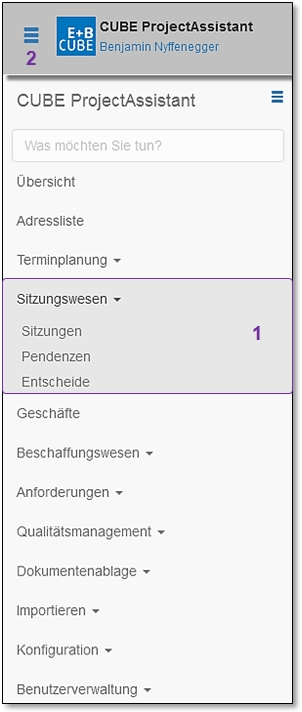
\includegraphics[height=150mm]{../chapters/01_Einfuehrung/pictures/1-3-1_Menuuebersicht_oSitzungswesen.jpg}
  \end{center}
  \vspace{-20pt}
  \caption{Das Menü}
  \vspace{-10pt}
\end{wrapfigure}
Die verschiedenen Bereiche des CUBE PA können Sie jederzeit über das Menü erreichen. Je nach Bereich können Sie zwischen verschiedenen Unterkategorien auswählen. Klicken Sie dazu auf das gewünschte Thema. Befinden sich darin weitere Unterthemen werden diese angezeigt. Unter „Sitzungswesen“ \col{(1)} werden die drei Unterkategorien „Sitzungen“, „Pendenzen“ und „Entscheide“ aufgelistet. Durch Mausklick auf die gewünschte Unterkategorie wird diese geöffnet. Mit erneutem Klick auf den Themenbereich (Sitzungswesen), klappen die Unterthemen wieder ein. 

\vspace{\baselineskip}

Mit Klick auf das Menü-Icon \col{(2)} können Sie das Menü ein- und ausblenden. So steht Ihnen eine grössere Arbeitsfläche zur Verfügung.

\vspace{6.5cm}  

\textbf{Angepasstes Menü}

\begin{wrapfigure}[7]{r}{5.5cm}
\vspace{-35pt}
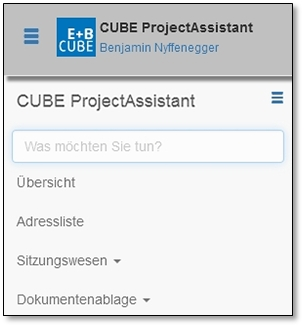
\includegraphics[height=60mm]{../chapters/01_Einfuehrung/pictures/1-3-1_MenuAngepasst.jpg}
\caption{Angepasstes Menü}
\end{wrapfigure}

Abhängig von den Berechtigungen, welche einem Nutzer gegeben werden, kann sich das Menü in der Vielfalt / den sichtbaren Menüpunkten zu den Printscreens in dieser Anleitung wie auch zu anderen Benutzern (andere Rollen, z.B. Administrator) unterscheiden. In der vorliegenden Anleitung werden jeweils sämtliche Menüpunkte abgebildet.

\subsubsection{Übersicht}
\label{bkm:Ref132000001}
Die persönliche Übersicht erscheint als erstes, wenn Sie sich beim CUBE PA angemeldet haben. Sie gibt einen schnellen Überblick über Sachverhalte, die Sie direkt betreffen. Die angezeigten Module sind abhängig von den Rollen, welche ein Benutzer erhält.

\begin{figure}[H] % Example image
\center{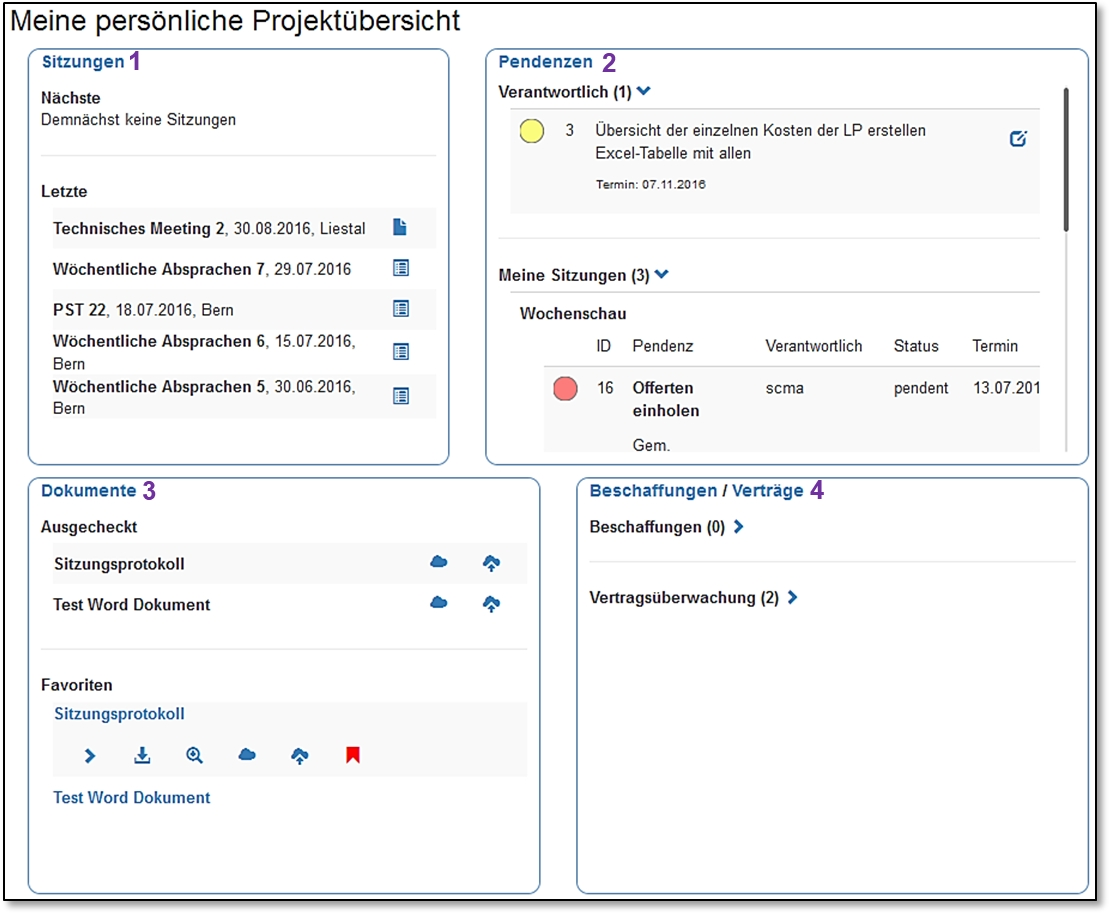
\includegraphics[width=1\linewidth]{../chapters/01_Einfuehrung/pictures/1-3-2_persUebersicht.jpg}}
\caption{Meine persönliche Projektübersicht}
% \label{fig:speciation}
\end{figure}

Oben links erscheinen die aktuellen Sitzungen \col{(1)}. Unter „Nächste“ erscheinen demnächst stattfindende Sitzungen mit Ihrer Beteiligung. Sie haben die Möglichkeit eine Sitzungseinladung zu bearbeiten oder für den Versand als pdf zu speichern. Unter „Letzte“ werden Sitzungen dargestellt, die kürzlich stattgefunden haben. Mit einem Klick können Sie das Protokoll öffnen. Ist noch kein definitives Protokoll vorhanden, können Sie dieses noch bearbeiten. Wenn Sie auf den blauen Titel „Sitzungen“ \col{(1)} klicken, wechseln Sie direkt in den Unterpunkt „Sitzungen“ der Rubrik „Sitzungswesen“.

\vspace{\baselineskip}

Oben rechts erscheinen die Pendenzen \col{(2)}, für die Sie verantwortlich oder bei deren Erledigung Sie beteiligt sind (Mitarbeit). Mit einem Klick können Sie eine Pendenz bearbeiten. Die entsprechende Maske wird geöffnet. Wenn Sie auf den blauen Titel „Pendenzen“ \col{(2)} klicken, wechseln Sie direkt in den Unterpunkt „Pendenzen“ der Rubrik „Sitzungswesen“. Siehe Kapitel 5.4 für das Erstellen und 5.5 für die Bearbeitung von Pendenzen.

\vspace{\baselineskip}

\begin{wrapfigure}[7]{r}{6.5cm}   % [x] Wie manche Zeile soll sich um die Grafik "brechen"
  \vspace{-15pt}      % Grundwert war 20; mit 30 schön oben beim Text ausgerichtet
  \begin{center}
    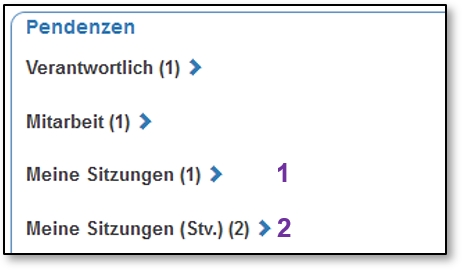
\includegraphics[width=1\linewidth]{../chapters/01_Einfuehrung/pictures/Sitzungsart_Zuweisung.jpg}
  \end{center}
  \vspace{-20pt}
%  \caption{CUBE PA konfigurieren}
  \vspace{-10pt}
\end{wrapfigure}

Werden für Anwender bestimmte Sitzungsarten in den Einstellungen als 'Vorsitz' oder 'Stv. Vorsitz' definiert, erscheinen diese Sitzungen ebenfalls in der persönlichen Projektübersicht als 'Meine Sitzungen' \col{(1)}, resp. 'Meine Sitzungen (Stv.)' \col{(2)}. Werden diese Positionen aufgeklappt, werden die in Zusammenhang mit dieser Sitzung stehenden Pendenzen eingeblendet.

\vspace{\baselineskip}

Links unten erscheinen für Sie relevante Dokumente \col{(3)}. Unter „Ausgecheckt“ werden die von Ihnen ausgecheckten Dokumente angezeigt. Sie haben die Möglichkeit ein ausgechecktes Dokument von hier aus zu öffnen oder es wieder einzuchecken. \\

Unter „Favoriten“ werden diejenigen Dokumente aufgelistet, die von Ihnen als persönliche Favoriten markiert wurden. Mit Klick auf den blauen Dokumententitel erscheinen die möglichen Optionen: Sie haben die Möglichkeit ein favorisiertes Dokument herunterzuladen, Details anzuschauen, den Eintrag zu ändern oder das Dokument auszuchecken, damit Sie es bearbeiten können und es während dieser Zeit für andere gesperrt ist. Ebenso können Sie ein favorisiertes Dokument in der Vorschau betrachten. Falls Sie ein Dokument nicht mehr als Favorit benötigen, klicken Sie auf das rote Flag-Symbol und der Eintrag verschwindet nach einem Aktualisieren der Ansicht oder erneutem Klick auf die 'Übersicht'. Mit erneutem Klick auf den Dokumententitel werden die Optionen zur besseren Übersicht wieder ausgeblendet. Wenn Sie auf den blauen Titel „Dokumente“ \col{(3)} klicken, wechseln Sie direkt in den Unterpunkt „Dokumente“ der Rubrik „Dokumentenablage“.

\vspace{\baselineskip}

% Text, welcher bis zur Grafik reichen soll, ist unmittelbar an Grafikeinbettung 
% zu schreiben, dann kommt Grafikeinbettung, dann Text, welcher Grafik umschliesst.

\begin{wrapfigure}{r}{0.5\textwidth}
  \vspace{-20pt}
  \begin{center}
    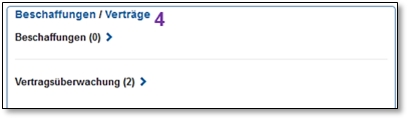
\includegraphics[width=0.5\textwidth]{../chapters/01_Einfuehrung/pictures/1-3-2_persUebersichtBeschaffung.jpg}
  \end{center}
  \vspace{-20pt}
%  \caption{Persönliche Übersicht}
  \vspace{-10pt}
\end{wrapfigure}
Weiter unten erscheinen die Beschaffungen \col{(4)} und Vertragsüberwachungen, an denen Sie beteiligt sind, und bei denen eine Aktion von Ihnen erwartet wird. In Klammern sehen Sie bei wie vielen Einträgen Sie involviert sind. Klicken Sie auf das horizontale Pfeilsymbol, um sich die Beschaffungen oder einer Vertragsüberwachung anzeigen zu lassen. Von hier aus können Sie mit Klick auf das Lupensymbol neben einer Beschaffung oder eine Vertragsüberwachung direkt in die entsprechende Beschaffung wechseln und diese dann bearbeiten. Je nach Stand der Beschaffung kann es aber sinnvoller sein via Menü und dem Punkt Beschaffungswesen und den dort vorhandenen Unterpunkte an die richtige Bearbeitungsmöglichkeit zu gelangen. Siehe Kapitel 7 über das Beschaffungswesen. Wenn Sie auf die blauen Titel „Beschaffungen“ resp. „Verträge“ \col{(4)} klicken, wechseln Sie direkt in die Unterpunkte „Beschaffungen“ resp. „Verträge“ der Rubrik „Beschaffungswesen“.

\pagebreak

In der Übersicht 'Pläne' \col{(5)} sehen Sie auf einen Blick, welche Planlieferungen (Druckauftrag via Reprozentrum) noch ausstehend sind. 

\begin{figure}[H] % Example image
\center{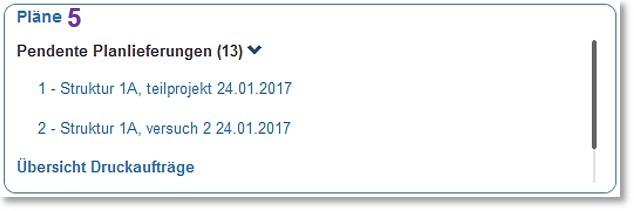
\includegraphics[width=.6\linewidth]{../chapters/01_Einfuehrung/pictures/1-3-2_UebersichtPlaene.jpg}}
\caption{Übersicht - Pläne}
% \label{fig:speciation}
\end{figure}

Mit Klick auf 'Übersicht Druckaufträge' wechseln Sie in den Menüpunkt 'Druckaufträge' (unter 'Dokumentenablage'). Dort finden Sie die Druckaufträge mit Detailinformationen. Weiter können Sie die bestellten Dokumente herunterladen, die Lieferscheine öffnen und Kostenübersichten zusammenstellen.

\vspace{\baselineskip}

\begin{wrapfigure}[5]{r}{0.5\textwidth}
  \vspace{-30pt}
  \begin{center}
    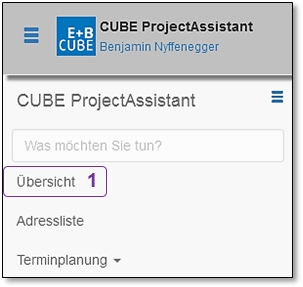
\includegraphics[width=0.4\textwidth]{../chapters/01_Einfuehrung/pictures/1-3-2_MenuepunktUebersicht.jpg}
  \end{center}
  \vspace{-20pt}
  \caption{Menü Übersicht}
  \vspace{-10pt}
\end{wrapfigure}
Wenn Sie mittels dem Menü in einen anderen Bereich wechseln, verlassen Sie die persönliche Übersicht. Um wieder dorthin zu gelangen, klicken Sie im Menü den Punkt „Übersicht“ \col{(1)}.

\vspace{4cm} 

\subsubsection{Adressliste}

In der Adressliste werden auf einfache Art und Weise sämtliche im CUBE PA erfassten Personen (Benutzer) und Firmen (Beteiligte) angezeigt. Mittels der Filterfunktion können die gesuchten Einträge rasch gefunden werden.

\subsubsection{Terminplanung}

Die Funktionalität ist derzeit rudimentär und beschränkt sich im Wesentlichen auf das Herunterladen von Dokumenten. Sie ist deshalb vorläufig nicht im Detail beschrieben. Beim 'Detailterminprogramm' handelt es sich um einen Microsoft-Project Import (xml-File), welcher dann ein Filtern und Anzeigen der eingelesenen Daten ermöglicht.

\subsubsection{Sitzungswesen}

Der CUBE PA unterstützt den vollständigen Workflow für das Einladen zu und das Protokollieren von Sitzungen, mit Ausnahme der Kalender- und Raumbuchungen, die typischerweise in Outlook erfolgen. Die für eine Sitzungseinladung erfassten Daten stehen automatisch als Grundlage für das Protokoll zur Verfügung. Dieses kann direkt im CUBE PA erfasst und von den Teilnehmern korrigiert werden. Ebenfalls steht eine Pendenz- und Entscheidverwaltung zur Verfügung.

\subsubsection{Geschäfte}

Der CUBE PA unterstützt ein einfach zu erfassendes, strukturiertes Projektjournal. Wird dieses gewissenhaft geführt, sind alle Projektbeteiligte immer und überall auf dem neuesten Stand der Dinge.

\subsubsection{Anforderungs- und Mängelmanagement}

Das 'Anforderungs- und Mängelmanagement' dient der Abnahme von Projekten. Sämtliche Mängel werden dokumentiert und mit 'Arbeitspaketen' und Pendenzen verknüpft. So haben Sie jederzeit den Überblick über eine Abnahme und wissen genau, welche Arbeiten noch erledigt oder nachgebessert werden müssen.

\subsubsection{Controlling}

Das Controlling unterstützt die Projektleitung hinsichtlich Kostenübersicht. Es werden Kontos angelegt, welche eine Referenz zu Beschaffungen haben. Eingehende Rechnungen werden erfasst und die Kostenübersicht wird nun in Bezug zum Budget einer Beschaffung dargestellt. 

\subsubsection{Beschaffungswesen}

Der CUBE PA unterstützt den vollständigen Workflow einer Beschaffung von der Offertanfrage über die Offerte und die Offertprüfung zum Vertrag. Die Verknüpfungen zwischen Offertanfrage, Offerte und Vertrag sind über ein intelligentes Nummerierungssystem einfach ersichtlich. Das Beschaffungswesen unterstützt dabei das freihändige Verfahren, das Einladungsverfahren und das offene Verfahren.

\subsubsection{Qualitätsmanagement / Handbücher}

Die Funktionalität des 'Qualitätsmanagements' ist derzeit rudimentär und beschränkt sich im Wesentlichen auf das Herunterladen von Dokumenten (z.B. Checklisten, Sicherheitsformulare etc.). Die Funktionalität 'Handbücher' ermöglicht das vollständige Erfassen von Projekt- oder anderen Handbücher im CUBE PA.

\subsubsection{Customer Relationship Management}

Das CRM (Customer Relationship Management) ermöglicht Ihnen effizient Veranstaltungen (Anlässe, Präsentationen und Schulungen) zu koordinieren. Es unterstützt Sie bei der Einladung, dem Verwalten von Anmeldungen, Versenden von Erinnerungen und dem Erstellen von Teilnehmerlisten. Für Ihre Veranstaltung erstellen Sie über eine Webseite eine Einladung in Form eines Online-Flyers, auf welchem sich die Teilnehmer an- oder abmelden können.

\subsubsection{Dokumentenablage}

Die Dokumentenablage ermöglicht das versionierte Ablegen von Dokumenten aller Art. Die abgelegten Dokumente können mit Metadaten / Tags gekennzeichnet werden. Nebst der Möglichkeit Dokumente ein- und auszuchecken und direkt in den Office-Programmen zu bearbeiten (wie bei Microsoft SharePoint), können die Dokumente online betrachtet werden (Vorschaufunktion). Jedes Dokument kann einem geografischen Ort zugewiesen werden (Doppelklick direkt in die Google-Map). Der Ort kann nachträglich per Drag’n’Drop in der Karte verschoben werden. Die Dokumentenablage ermöglicht eine Übersicht über geografisch benachbarte Dokumente.

\subsubsection{Importieren}

Mittels dieser Option können Adresslisten, Terminpläne und Geschäfte (Daten) importiert werden.

\subsubsection{Konfiguration}

Die Konfiguration dient dazu, projektspezifische Daten zu erfassen, die anschliessend in Auswahllisten erscheinen sollen. Diese Arbeit muss normalerweise nur von wenigen Personen gemacht werden (Superuser, Administratoren) und wird deshalb nur rudimentär beschrieben.

\subsubsection{Benutzerverwaltung}

In der Benutzerverwaltung werden Benutzer, Teams sowie Gruppen erfasst.




\section{Getting started}
\subsection{Zugangsberechtigung einholen / neues Passwort anfordern}

% Die Zugangsberechtigung zum CUBE PA erhalten Sie für das Projekt Zugkunft Waldenburgerbahn beim Gesamtleiter. Senden Sie
% eine E-Mail an folgende Adresse (Zeitpunkt der Aufschaltung wird noch bekanntgegeben):

Die Zugangsberechtigung zum CUBE PA erhalten Sie jeweils über den Projektverantwortlichen. Bei Fragen bezüglich den Zuständigkeiten oder dem Freischalten eines CUBE PA-Zugangs können Sie sich an folgende Email-Adresse wenden:

\vspace{\baselineskip}

% \href{mailto:cube.support@emchberger.ch}{\textstyleInternetlink{cube.support@emchberger.ch}}
{\color{red} cube.support@emchberger.ch}

\vspace{\baselineskip}

Falls Sie Ihr Passwort vergessen haben, können Sie auf der Login-Seite des CUBE PA mittels der Funktion 'Passwort vergessen' ein neues Passwort anfordern, resp. wird Ihnen ein Link zugestellt, mit welchem Sie ein neues Passwort setzen können. Bei Fragen können Sie sich ebenfalls an obige Email-Adresse wenden.

\vspace{\baselineskip}

Aus Sicherheitsgründen empfehlen wir, per E-Mail erhaltene Passwörter sofort zu ändern.

\subsection{Internetverbindung}

Eine funktionierende Internetverbindung ist eine Voraussetzung für die Benutzung des CUBE PA. Offline Arbeiten wird nicht unterstützt, da alle Daten auf einem Server gespeichert sind.

\vspace{\baselineskip}

Falls Sie beim Benutzen des CUBE PA unerwartete Probleme feststellen, beachten Sie das Statussymbol der Verbindung unten rechts auf dem Bildschirm. Falls dieses rot ist, ist die Internet-Verbindung unterbrochen. Falls Ihnen dies während dem Erfassen von Daten passiert, versuchen Sie, die Internetverbindung wieder herzustellen und wenn dies gelingt, klicken Sie auf 'Übernehmen', um die im lokalen Arbeitsspeicher des CUBE PAs vorhandenen Daten zu sichern. Falls es auf die Schnelle nicht gelingt die Internet-Verbindung wieder herzustellen, verlassen Sie den CUBE ProjectAssistant nicht, und schalten Sie den Computer nicht aus. Suchen Sie einen anderen Standort, wo Sie eine Internet-Verbindung herstellen
können und sobald eine solche vorhanden ist, klicken Sie auf 'Übernehmen'.

\vspace{\baselineskip}

\textbf{Status der Verbindung:}

\vspace{\baselineskip}

\begin{tabular}{c | p{14cm} l} %{cl}

\vspace{+1pt}	

\includegraphics[height=12pt] {/Icons/online.jpg} & Sie haben eine Internet-Verbindung und sind im CUBE PA angemeldet. \\
\vspace{+1pt}	

\includegraphics[height=12pt]{/Icons/offline.jpg} & Die Internet-Verbindung ist unterbrochen oder der CUBE PA-Server ist vorübergehend nicht erreichbar. \\
\vspace{+1pt}	

\includegraphics[height=12pt]{/Icons/abgemeldet.jpg} & Sehen Sie kein Statussymbol haben Sie eine Internet-Verbindung, sind aber nicht im CUBE PA angemeldet. \\

% 
\includegraphics[height=12pt]{/Icons/BlaueWolke_Blitz.jpg} & Sie haben eine Internet-Verbindung, sind aber nicht in CUBE PA angemeldet \\

\end{tabular}

\vspace{\baselineskip}

Falls Sie den CUBE PA verlassen während die Internet-Verbindung unterbrochen ist, gehen die zuletzt erfassten Daten verloren.

\subsection{CUBE PA starten}

% Benutzerspezifisch

Der Zugriff auf CUBE PA erfolgt über die folgende Adresse:

\vspace{\baselineskip}

{\color{red} http://www.cubetools.ch/}

\vspace{\baselineskip}

Sie gelangen auf die Startseite der CUBE Tools:

\begin{figure}[H]
\center{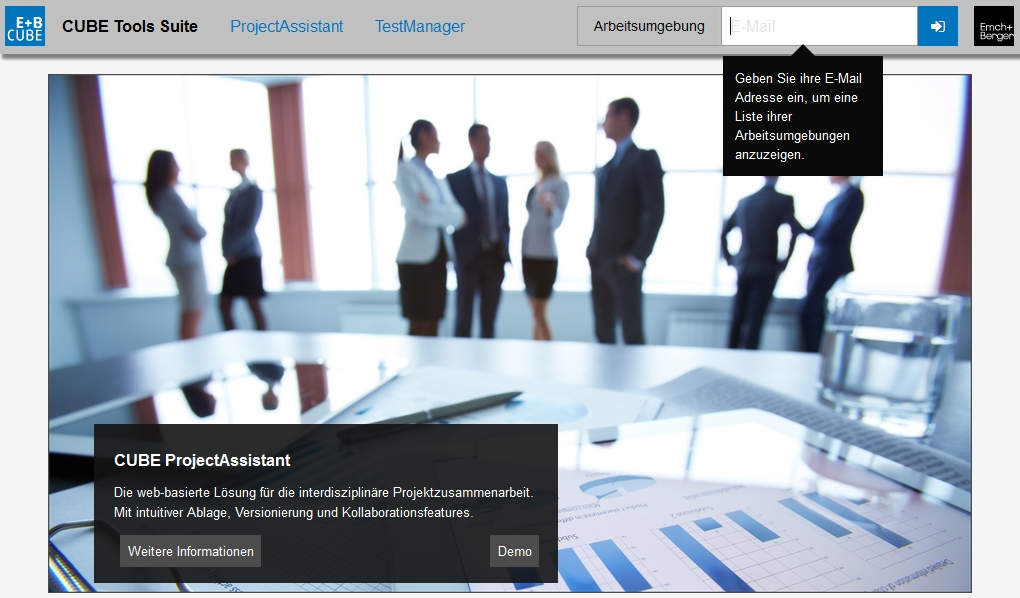
\includegraphics[width=.9\linewidth]{../chapters/02_GettingStarted/pictures/2-3_Einstiegsseite.jpg}}
\caption{Die Einstiegsseite für den CUBE PA}
% \label{fig:speciation}
\end{figure}

Geben Sie oben rechts im Fenster Ihre Email-Adresse ein und klicken Sie auf den blauen Pfeil-Button neben der eingegebenen Emailadresse:

\begin{figure}[H]
\center{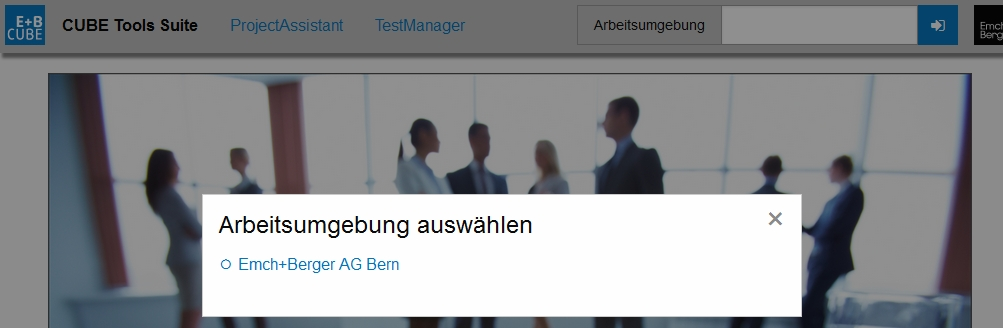
\includegraphics[width=.8\linewidth]{../chapters/02_GettingStarted/pictures/2-3_Arbeitsumgebung_auswaehlen.jpg}}
\caption{Die Arbeitsumgebung auswählen}
% \label{fig:speciation}
\end{figure}

Es werden sämtliche Arbeitsumgebungen angezeigt, bei welchen Sie registriert sind. Im Suchfeld können Sie nach der gewünschten Arbeitsumgebung suchen. Klicken Sie auf die entsprechende Arbeitsumgebung. Sie gelangen nun auf die Anmeldemaske:

\begin{figure}[H]
\center{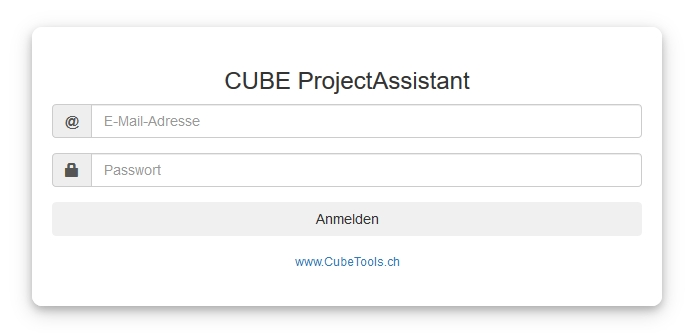
\includegraphics[width=0.5\linewidth]{../chapters/02_GettingStarted/pictures/2-3_CUBEPA_Anmeldung.jpg}}
\caption{An CUBE PA anmelden}
% \label{fig:speciation}
\end{figure}

Geben Sie Ihre E-Mail Adresse und das Passwort ein. Nach Klick auf 'Anmelden' erscheint die persönliche Übersicht.

\vspace{\baselineskip}

\textbf{Hinweis:} Wenn Sie noch nicht registriert sind, können Sie mit Klick auf den Link 'Registrierung' einen Zugang beantragen. Füllen Sie das Formular aus und klicken Sie auf den Button 'Registrieren'.

\vspace{\baselineskip}

\textbf{Hinweis:} Haben Sie in Ihrem Browser gültige Zugangsdaten (E-Mail Adresse und Passwort) hinterlegt, werden Sie direkt in CUBE PA eingeloggt.

\subsection{Passwort ändern}
\label{bkm:Ref434828103}

Aus Sicherheitsgründen empfehlen wir Ihnen jedes Passwort, dass Sie per E-Mail erhalten haben, sofort zu ändern. Klicken Sie dazu oben links im Bildschirm auf ihren Namen. Es wird ein Menü geöffnet, welches Ihnen ermöglicht sich beim CUBE PA abzumelden, das Passwort zu ändern oder das vorliegende Handbuch zu öffnen oder zu speichern.

\begin{figure}[H]
\center{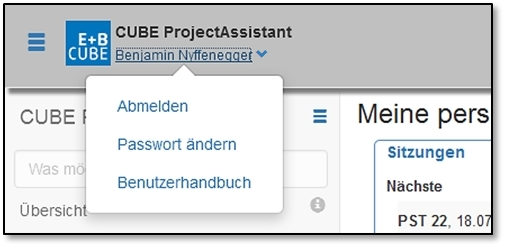
\includegraphics[width=0.5\linewidth]{../chapters/02_GettingStarted/pictures/2-4_Passwort_aendern.jpg}}
\caption{Das Passwort ändern}
% \label{fig:speciation}
\end{figure}

Mit Klick auf 'Passwort ändern' erscheint eine Maske, in der Sie einmal das alte Passwort und zweimal das neue Passwort eingeben müssen:

\begin{figure}[H]
\center{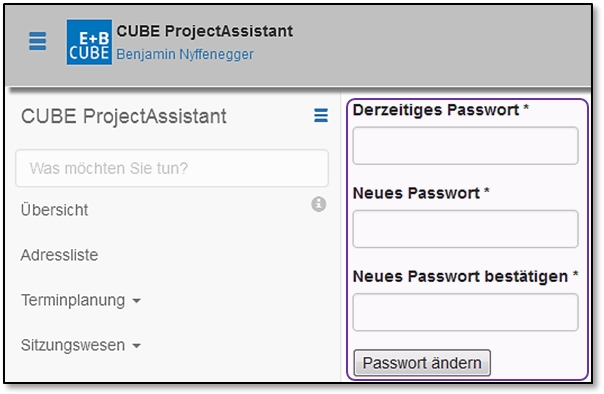
\includegraphics[width=0.5\linewidth]{../chapters/02_GettingStarted/pictures/2-4_Passwort_Eingabe.jpg}}
\caption{Neues Passwort eintragen}
% \label{fig:speciation}
\end{figure}

Sobald Sie die Schaltfläche 'Passwort ändern' anklicken, gilt das neue Passwort.

\subsection{Die wichtigsten Menüs, Schaltflächen, Symbole und Hinweise in Kürze}

Die Bedienung des CUBE PA orientiert sich an der gebräuchlichen Bedienung von Internet-Applikationen. Wer regelmässig ein Smartphone oder ein Tablet benutzt, wird sich im CUBE PA schnell zurechtfinden.

\vspace{\baselineskip}

In diesem Kapitel werden die wichtigsten Menüs, Schaltflächen und Symbole erläutert, die in allen Teilen des CUBE PA erscheinen und immer die gleiche Bedeutung haben.

\pagebreak

\subsubsection{Menüs}

\begin{figure}[H]
\center{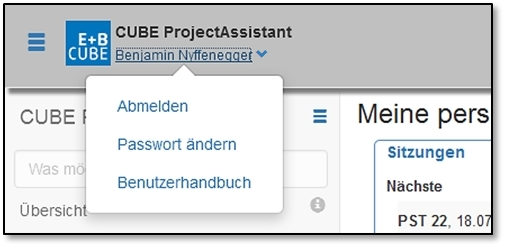
\includegraphics[width=0.5\linewidth]{../chapters/02_GettingStarted/pictures/2-4_Passwort_aendern.jpg}}
\caption{Das Eingangsmenü}
% \label{fig:speciation}
\end{figure}


Oben links sehen Sie jeweils, wer im CUBE PA angemeldet ist. Mit Klick auf den Namen öffnen sich weitere Optionen. Das Wechseln des Passwortes wurde oben beschrieben (Kapitel \ref{bkm:Ref434828103}). Sie haben mit Klick auf 'Benutzerhandbuch' die Möglichkeit das vorliegende Handbuch per pdf zu öffnen oder zu speichern. Wenn Sie auf 'Abmelden' klicken, verlassen Sie den CUBE PA ohne Umschweife, ausser sie hätten neu erfasste Daten noch nicht gespeichert. In diesem Fall erscheint eine Warnung:

\begin{figure}[H]
\center{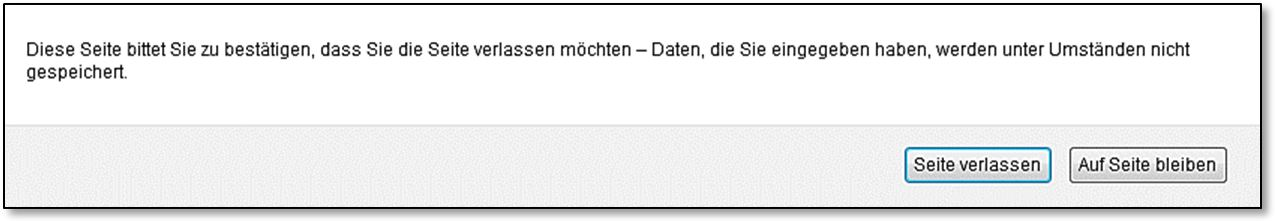
\includegraphics[width=1\linewidth]{../chapters/02_GettingStarted/pictures/251_Browsermeldung.jpg}}
\caption{Browser-Warnung}
% \label{fig:speciation}
\end{figure}
\begin{small}
Der Inhalt dieser Meldung ist abhängig vom verwendeten Browser (hier Firefox) und somit nicht beeinflussbar.
\end{small}

\vspace{\baselineskip}

Sie können das Verlassen des CUBE PA abbrechen (Auf Seite bleiben) und die noch nicht gespeicherten Daten sichern, indem Sie auf 'Übernehmen' klicken.

\vspace{\baselineskip}

\pagebreak

Links befindet sich das Hauptmenü:

\vspace{\baselineskip}

\begin{wrapfigure}[20]{l}{6.5cm}   % [x] Wie manche Zeile soll sich um die Grafik "brechen"
  \vspace{-35pt}      % Grundwert war 20; mit 30 schön oben beim Text ausgerichtet
  \begin{center}
    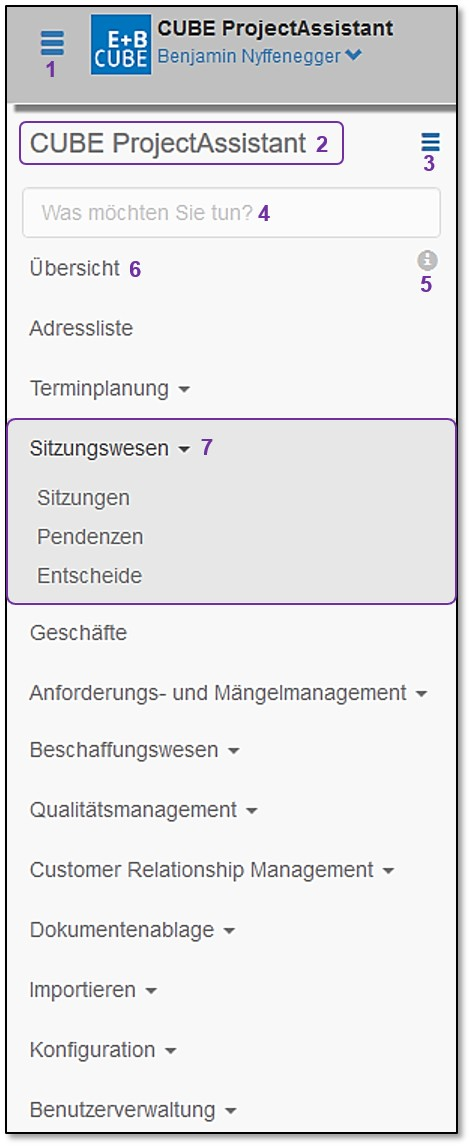
\includegraphics[width=1\linewidth]{../chapters/02_GettingStarted/pictures/2-5-1_Menu_Uebersicht.jpg}
  \end{center}
  \vspace{-20pt}
  \caption{Das Menü verwenden}
  \vspace{-10pt}
\end{wrapfigure}

Das Menü ermöglicht die Auswahl sämtlicher Themen, für welche Sie berechtigt sind. Entsprechend kann sich die Abbildung zu Ihrem Menü unterscheiden. Ebenso ist es möglich, dass sich innerhalb eines Menü die Unterpunkte (Hier z. B. 'Externe Sitzungen' beim Sitzungswesen) unterscheiden, da kundenspezifisch weitere Menüpunkte konfiguriert werden können. Die Grundfunktionen sind aber dieselben. Mit Klick auf das Menü-Icon \col{(1)} können Sie jeweils das gesamte Menü ein- und ausblenden. Damit gewinnen Sie bei Bedarf eine grössere Arbeitsfläche in Ihrem Browser. \\
Die Bezeichnung unter \col{(2)} zeigt Ihnen die aktuelle Arbeitsumgebung an. Mit Klick auf das Icon \col{(3)} können Sie die Arbeitsumgebung direkt wechseln. 

\vspace{\baselineskip}

\begin{raggedleft}
\hspace{80mm} 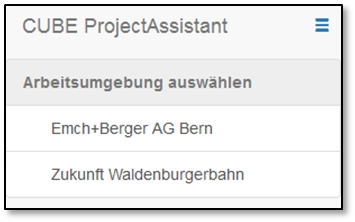
\includegraphics[height=40mm]{../chapters/02_GettingStarted/pictures/2-5-1_Arbeitsumgebung_wechseln.jpg}
\end{raggedleft}

\vspace{\baselineskip}

Es werden Ihnen natürlich nur diejenigen Arbeitsumgebungen angezeigt, für welche Sie eine Berechtigung haben. Mit Klick auf die gewünschte Arbeitsumgebung kommen Sie zum Anmeldefenster der entsprechenden Arbeitsumgebung. Falls Sie an diesem Tag (ohne den Computer neu gestartet zu haben) eine Arbeitsumgebung bereits mal geöffnet hatten, gelangen Sie ohne Anmeldung wieder in die gewünschte Umgebung. Mit Klick auf das gleiche Symbol \col{(3)} schliessen Sie diese Auswahl wieder. 

\vspace{\baselineskip}

Ein zentrales Werkzeug ist das Such-Feld 'Was möchten Sie tun?' \col{(4)}. Hilfreich für eine zielführende und effektive Anwendung sind die Informationen, welche Sie mit dem Info-Icon \col{(5)} erhalten:

\begin{figure}[H]
\center{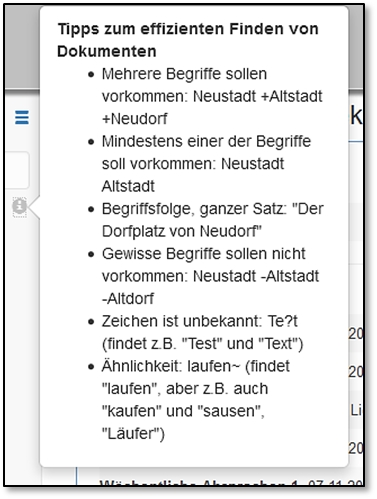
\includegraphics[width=0.35\linewidth]{../chapters/02_GettingStarted/pictures/2-5-1_Hilfe_zu_Suche.jpg}}
\caption{Tipps für eine effektive Suche}
% \label{fig:speciation}
\end{figure}

Wenn Sie irgendwo in das Browserfenster klicken, schliesst das Info-Fenster wieder. Geben Sie ins Such-Feld \col{(4)} den oder die gewünschten Begriff/e ein. CUBE PA durchsucht alle Menüthemen und Einträge, sowie auch Inhalte von hochgeladenen Dokumenten (z.B. Word und PDF). \\

\textbf{Wichtig zu beachten} ist, dass PDF-Dokumente nur durchsucht werden können, wenn es sich auch um integrierten Text und nicht um Bilder handelt. Wurde ein Text gescannt und als Bild in einem PDF gespeichert, wird dieser Inhalt nicht durchsucht.\\

\begin{wrapfigure}[14]{r}{7cm}   % [x] Wie manche Zeile soll sich um die Grafik "brechen"
  \vspace{-30pt}      % Grundwert war 20; mit 30 schön oben beim Text ausgerichtet
  \begin{center}
    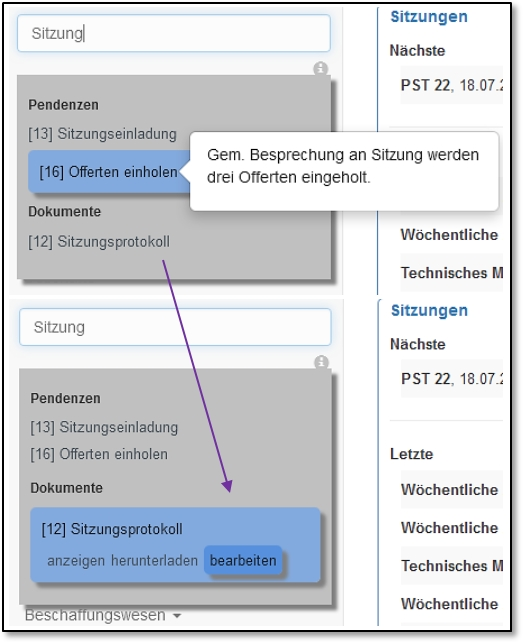
\includegraphics[width=0.8\linewidth]{../chapters/02_GettingStarted/pictures/2-5-1_Such_Ergebnisse.jpg}
  \end{center}
  \vspace{-20pt}
  \caption{Suchergebnisse verwenden}
  \vspace{-10pt}
\end{wrapfigure}

Alle gefundenen Übereinstimmungen werden nun angezeigt:

\begin{compactitem}
	\item Unter dem Stichwort wurden Einträge bei den Pendenzen und bei den Dokumenten gefunden.
	\item Fahren Sie mit der Maus über einen Eintrag der Pendenzen, erscheinen Details zu 'Offerten einholen'.
	\item Unter anderen Themen, hier unter Dokumente, haben Sie die Möglichkeit das gefundene Dokument (hier ein Sitzungsdokument) anzeigen zu lassen, herunterzuladen oder zu bearbeiten. Dazu fahren Sie mit der Maus über die gewünschte Option. Diese wird dann hervorgehoben und mit einem Mausklick ausgeführt.
\end{compactitem}

\vspace{\baselineskip}

Mit dem Menüpunkt 'Übersicht' \col{(6)} gelangen Sie immer wieder zurück auf die persönliche Übersichtsseite. Sind unter einem Menüpunkt weitere Unterpunkte vorhanden, wird dies mit einem kleinen Dreieck angezeigt. Wenn Sie auf den Titel klicken, werden die Untermenüs sichtbar \col{(7)}. Der Hauptpunkt 'Sitzungswesen' ist selbst nicht verlinkt. Mit erneutem Klick darauf schliessen die Unterpunkte wieder.

\vspace{\baselineskip}

Das Haupt-Menü gibt Zugang zu den verschiedenen Teilen des CUBE PA. Je nach erteilten Benutzerrechten sind nicht alle Rubriken für alle Benutzer sichtbar und zugänglich.

\begin{itemize}
\item
\textbf{Übersicht}: zeigt die für Sie relevanten Sitzungen, Pendenzen, Dokumente und Beschaffungen an.
\item
\textbf{Adressliste: }Anzeigen der erfassten Adressen mit Filterfunktion. Hier können auch neue Einträge (Personen und Organisationen) angelegt werden.
\item
\textbf{Terminplanung}: Anzeigen und Bearbeiten von Terminplänen.
\item
\textbf{Sitzungswesen}: Anzeigen und Bearbeiten von Sitzungseinladungen, Sitzungsprotokollen, Pendenzen und
Entscheiden.
\item
\textbf{Geschäfte}: Unterstützung für ein einfach zu erfassendes, strukturiertes Projektjournal.
\item
\textbf{Projekt- / Anforderungsmanagement}: Unterstützung bei der Abnahme von Projekten. Überblick über offene Arbeitspakete und Nachbesserungen.
\item
\textbf{Beschaffungswesen}: Abwickeln von Beschaffungen, von der Ausschreibung bis zum Vertragsabschluss.
\item
\textbf{Qualitätsmanagement}: Zugriff auf Dokumente über Risikomanagement und Nahtstellen. Hier können Sie auch ein Projekthandbuch oder andere Handbücher erstellen.
\item
\textbf{Customer Relationship Managemen}: Das CRM (Customer Relationship Management) ermöglicht Ihnen effizient Veranstaltungen (Anlässe, Präsentationen und Schulungen) zu koordinieren.
\item
\textbf{Dokumentenablage}: Dokumenten-Management mit Online-Ansicht. Geänderte Dokumente werden mit einer neuen Versionsnummer abgelegt.
\item
\textbf{Importieren}: Importieren von Daten (Termine und Geschäfte).
\item
\textbf{Konfiguration}: Hier werden die Inhalte der Auswahllisten festgelegt und angepasst.
\item
\textbf{Benutzerverwaltung}: Verwalten von Benutzern, Teams und Gruppen.
\end{itemize}

% bishierher

\subsubsection{Schaltflächen}

Die folgenden Schaltflächen kommen immer wieder vor:

\vspace{\baselineskip}

% 2.8, 12

\begin{tabular}{|c | p{10cm}|l} %{cl}
\hline
\raisebox{-1\totalheight}{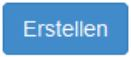
\includegraphics[height=20pt]{/Icons/B_Erstellen.jpg}} & Erstellen: Durch Klicken auf diese Schaltfläche speichern Sie einen neu erfassten Datensatz zum ersten Mal, was Ihnen dann die Möglichkeit zur weiteren Bearbeitung öffnet. \\
\hline
\raisebox{-1\totalheight}{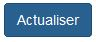
\includegraphics[height=20pt]{/Icons/B_Uebernehmen.jpg}} & Übernehmen: Wenn Sie auf diese Schaltfläche klicken, bewirken Sie, dass kürzlich erfasste oder geänderte Daten, die bis jetzt nur im Arbeitsspeicher ihres Computers vorhanden sind, auf dem Server gesichert werden. \\
\hline
\raisebox{-1\totalheight}{
\includegraphics[height=20pt]{/Icons/Lupe_s.jpg}} & Lupe: Durch Klicken auf diese Lupe filtern Sie eine Liste, nachdem Sie in den Feldern auf der ersten Zeile der Liste die Filterkriterien ausgewählt oder einen Suchbegriff eingegeben haben. \\
\hline
\raisebox{-1\totalheight}{
\includegraphics[height=20pt]{/Icons/FilterLoeschen.jpg}} & Filter löschen: Durch Klicken auf dieses Symbol werden sämtliche Eingaben in den Suchfeldern gelöscht. \\
\hline
\raisebox{-1\totalheight}{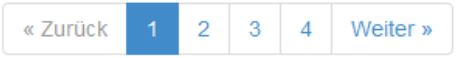
\includegraphics[height=16pt]{/Icons/weitereSeiten.jpg}} & Blättern in Liste: mit dieser Schaltfläche können Sie in einer Liste vorwärts oder zurückblättern, in dem Sie auf 'Weiter' oder 'Zurück' klicken, oder eine bestimmte Seite auswählen, indem Sie auf die Seitennummer klicken. Falls die Liste mehr als fünf Seiten umfasst, werden nicht alle Seitennummern angezeigt. Klicken Sie auf 'Weiter' oder 'Zurück' bis die gewünschte Seite angewählt werden kann.  \\
\hline
\end{tabular}

\begin{figure}[H]
\center{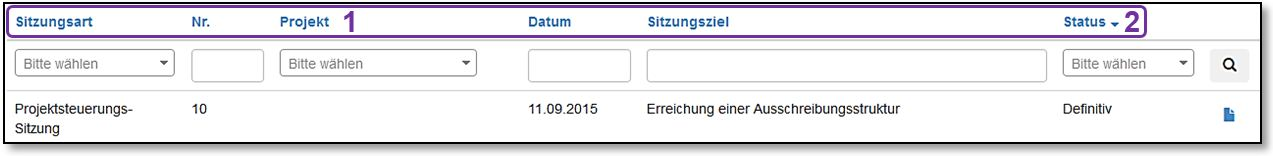
\includegraphics[width=1\linewidth]{252_Listen_sortieren.jpg}}
\caption{Spalten: Inhalt sortieren}
% \label{fig:speciation}
\end{figure}


Zusätzlich haben alle in blau erscheinenden Spaltentitel von Listen die Wirkung einer Schaltfläche \col{(1)}. Durch Klicken auf einen Spaltentitel sortieren Sie die
Liste in aufsteigender Reihenfolge bezüglich dieser Spalte. Durch erneutes Klicken auf den Spaltentitel kehren Sie die Reihenfolge um. Das kleine Dreieck 
\includegraphics[height=10pt]{/Icons/welcheSpalte_sort.jpg} \col{(2)} zeigt einerseits nach welcher Spalte sortiert wird (hier nach 'Status') und andererseits wie die Reihenfolge der Sortierung ist: (Sortierung A {\textgreater} Z 
\includegraphics[height=10pt]{/Icons/Status_down.jpg} resp. Z {\textgreater} A 
\includegraphics[height=10pt]{/Icons/Status_up.jpg}).

\pagebreak
\subsubsection{Symbole}
\label{bkm:Ref443039356}
Die folgenden Symbole haben überall im CUBE PA dieselbe Bedeutung. Solche Schaltflächen und Textlinks wechseln in der Regel die Farbe, wird der Mauszeiger darüber bewegt. (Gilt nicht für die Statussymbole der Verbindung). 

\begin{tabular}{|c|p{14cm}|} %{cl}
\hline
\raisebox{-0.5\totalheight}{
\includegraphics[height=12pt]{/Icons/online.jpg}} & Unten links im Fenster sehen Sie die grünen Pfeilen. Dies bedeutet, Sie haben eine Internet-Verbindung und sind in CUBE PA angemeldet. \\

\includegraphics[height=12pt]{/Icons/offline.jpg} & Werden die Pfeile rot angezeigt, ist die Internetverbindung unterbrochen oder der CUBE PA-Server vorübergehend nicht erreichbar. \\

\includegraphics[height=12pt]{/Icons/abgemeldet.jpg} & Sehen Sie keine Pfeile, sind Sie aktuell an keiner Arbeitsumgebung in CUBE PA angemeldet. \\
\hline
\raisebox{-1\totalheight}{
\includegraphics[height=12pt]{/Icons/Plussymbol.jpg}} & Dieses Pluszeichen steht jeweils oben links im Fenster. Durch Klicken können Sie einen neuen Datensatz erstellen (z.B. eine neue Sitzungseinladung erfassen). \\
\hline
\raisebox{-1\totalheight}{
\includegraphics[height=12pt]{/Icons/Filter.jpg}} & Mit Klick auf dieses Symbol öffnen sich weitere Filtermöglichkeiten. Diese Filtereinstellungen lassen sich abspeichern und später wieder aufrufen. \\
\hline
\raisebox{-1\totalheight}{
\includegraphics[height=12pt]{/Icons/Nadelsymbol.jpg}} & Mit Klick auf das Nadelsymbol wird die Google-Maps ein- respektive wieder ausgeblendet. \\
\hline
\raisebox{-1\totalheight}{
\includegraphics[height=12pt]{/Icons/Listensymbol_zurueck.jpg}} & Mit diesem Listensymbol kehren Sie zurück zur Übersicht. Meist wird dieses Symbol angezeigt, wenn Sie sich mittels Lupe (Ansicht) oder Stift (Bearbeiten) in einem einzelnen Datensatz befinden. \\
\hline
\raisebox{-1\totalheight}{
\includegraphics[height=12pt]{/Icons/SpaltenEinst.jpg}} & Mit Klick auf dieses Konfigurationssymbol können Sie für Ihre Ansicht Spalten ein- und ausblenden. Für nicht benötigte Spalten nehmen Sie das Häkchen raus. \\
\hline
\raisebox{-1\totalheight}{
\includegraphics[height=12pt]{/Icons/Stift.jpg}} & Der Bleistift steht jeweils in der linke Ecke neben einem Feld \col{(1)} in einer Liste. Sie können nach einem Klick auf den Bleistift den Inhalt dieses Felds bearbeiten.   
\includegraphics[height=14pt]{253_Datum_edit.jpg}\\
\hline
\raisebox{-1\totalheight}{
\includegraphics[height=12pt]{/Icons/Gutzeichen.jpg}} & Wurden in einer Eingabemaske Änderungen vorgenommen, werden diese mit Klick auf das Gutzeichen gespeichert. \\
\hline
\raisebox{-1\totalheight}{
\includegraphics[height=12pt]{/Icons/Bearbeiten.jpg}} & Bleistift in Quadrat (klein): Mit einem Klick auf dieses Symbol öffnen Sie eine Maske, die das Bearbeiten sämtlicher Felder des entsprechenden Eintrages erlaubt. \\
\hline
\raisebox{-1\totalheight}{
\includegraphics[height=12pt]{/Icons/Pluszeichen.jpg}} & Pluszeichen: Durch einen Klick auf ein Pluszeichen können Sie einen neuen Eintrag in einer Liste erstellen, z.B. einen zusätzlichen Teilnehmer für eine Sitzungseinladung erfassen, Anhänge hinzufügen oder einer Person / Gruppe zusätzlich Berechtigungen erteilen. \\
\hline
\raisebox{-1\totalheight}{
\includegraphics[height=12pt]{/Icons/Lupe.jpg}} & Lupe: Dieses Symbol steht unmittelbar bei einer Zeile / einem Eintrag in einer Liste. Mit einem Klick darauf öffnen Sie eine Maske, die das Lesen des Inhalts aller Felder des entsprechenden Datensatzes erlaubt. \\
\hline
\raisebox{-1\totalheight}{
\includegraphics[height=12pt]{/Icons/Blattsymbol.jpg}} & Blatt mit Eselsohr oben rechts: Dieses Symbol kommt in einem Listenfeld vor. Durch einen Klick auf das Symbol können Sie eine PDF-Datei generieren. Der Spaltentitel sagt aus, welchen Inhalt das PDF-Dokument aufweist. \\
\hline
\end{tabular}

\pagebreak

\begin{tabular}{|c|p{14cm}|} %{cl}
\hline
\raisebox{-1\totalheight}{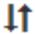
\includegraphics[height=12pt]{/Icons/VertPfeile.jpg}} & Gegenläufige vertikale Pfeile: Wenn Sie dieses Symbol mit gedrückt gehaltener linker Maustaste packen, können Sie diese Zeile innerhalb einer Liste nach oben oder unten verschieben und so die Reihenfolge der Einträge verändern. \\
\hline
\raisebox{-1\totalheight}{
\includegraphics[height=12pt]{/Icons/Muelltonne.jpg}} & Mülltonne: Durch einen Klick auf dieses Symbol können Sie eine Zeile einer Liste samt den zugehörigen Daten löschen. Z.B. löschen Sie so die Angaben zu einer Beilage und die Beilage selbst. Es erscheint eine Sicherheitsmeldung „Entfernen?“ Mit der Bestätigung auf „OK“ veranlassen Sie das Löschen der Daten. \\
\hline
\raisebox{-1\totalheight}{\includegraphics[height=12pt]{/Icons/Kreuzchen.jpg}} & Kreuzchen in Feldern: Durch Klicken auf das Kreuzchen am rechten Rand eines Felds löschen Sie den Inhalt eines Feldes mit Auswahlliste. \\
\hline
\raisebox{-1\totalheight}{\includegraphics[height=12pt]{/Icons/Pfeil_rechts.jpg}} & Horizontales Pfeilsymbol: Mit einem Klick darauf klappen Sie einen Inhalt aus (machen ihn sichtbar). \\
\hline
\raisebox{-1\totalheight}{\includegraphics[height=12pt]{/Icons/Pfeil_unten.jpg}} & Vertikales Pfeilsymbol: Mit einem Klick darauf klappen Sie einen Inhalt ein (machen ihn unsichtbar). \\
\hline
\raisebox{-1\totalheight}{\includegraphics[height=12pt]{/Icons/Verknuepfen.jpg}} & Ein bestehendes Dokument aus der Dokumentenablage verknüpfen. \\
\hline
\raisebox{-1\totalheight}{\includegraphics[height=12pt]{/Icons/ListeGenerieren.jpg}} & Mittels dieses Icons können Sie aus verschiedenen Ansichten / Modulen eine Excelliste generieren. \\
\hline
\end{tabular}

\subsubsection{Warnungen und Hinweise}

\textbf{Webseite verlassen ohne Daten zu speichern:} \\
Wenn Sie im CUBE PA Daten-Felder ausgefüllt haben und ohne Klicken auf 'Übernehmen' oder 'Erstellen' die aktuelle Seite verlassen wollen, erscheint folgende Meldung: 

\begin{figure}[H]
\center{\includegraphics[width=1\linewidth]{251_Browsermeldung.jpg}}
\caption{Browser-Warnung}
% \label{fig:speciation}
\end{figure}
\begin{small}
Der Inhalt dieser Meldung ist abhängig vom verwendeten Browser (hier Firefox) und somit nicht beeinflussbar.
\end{small}

\vspace{\baselineskip}

Sie haben die Möglichkeit durch Klicken 'Auf Seite bleiben' zurückzukehren und durch Klicken auf 'Übernehmen' oder 'Erstellen' die Daten zu sichern. Andererseits gehen die Daten verloren.

\vspace{\baselineskip}

\textbf{Pflichtfelder:}\\
Bei der Eingabe von Daten gibt es Pflichtfelder, welche zwingend ausgefüllt werden müssen. Wird ein solches Pflichtfeld übersehen, erscheint folgende Meldung:

\begin{figure}[H]
\center{\includegraphics[width=1\linewidth]{254_WarnungPflichfelder}}
\caption{Warnung Eingabe bei Pflichtfeld}
% \label{fig:speciation}
\end{figure}

Mit roter Schrift wird dann jeweils das Feld bezeichnet, welches ausgefüllt werden muss (Dieses Feld ist ein Pflichtfeld). Die Hinweismeldung kann mittels 'OK' weggeklickt werden. Erst nach einer Eingabe ist es möglich die Daten zu speichern und z.B. ein neues Dokument anzulegen. 

\vspace{\baselineskip}

\textbf{Speichern/Übernehmen während dem Hochladen von Dateien:}\\
Laden Sie in der Dokumentenablage eine grössere Datei hoch, kann das einige Zeit in Anspruch nehmen. Wollen Sie während dem Hochladen bereits die Eingaben speichern, erscheint eine Meldung, dass noch gerade Dateien hochgeladen werden. Warten Sie bis das Hochladen abgeschlossen ist (Fortschritt = 100 \%), danach können Sie auch 'Übernehmen' klicken. Meldung:

\begin{figure}[H]
\center{\includegraphics[width=.6\linewidth]{../chapters/02_GettingStarted/pictures/2-5-4_MeldungHochladen}}
\caption{Warnung beim Speichern während dem Hochladen einer Datei}
% \label{fig:speciation}
\end{figure}


\pagebreak
\subsection{CUBE PA auf mobilen Endgeräten (Smartphones, Tablets)}

CUBE PA kann auch auf mobilen Endgeräten wie Smartphones und Tablets verwendet werden. CUBE PA erkennt, dass es sich um ein mobiles Gerät handelt und schaltet automatisch auf die 'mobile' Ansicht um. Diese beinhaltet eine etwas abweichende Darstellung sowie angepasste Menüführung (siehe unten). Wird jedoch mit Tablets gearbeitet, auf welchen ein reguläres Windows-Betriebssystem installiert ist (z.B. Win 8.1 / Win 10 auf Microsoft Surface), wird die Ansicht nicht umgestellt, entsprechend lässt sich CUBE PA aktuell nicht oder nur umständlich mit Touch-Eingaben bedienen.


\begin{figure}[H]
\center{\includegraphics[width=1\linewidth]{26_Mobile_Ansicht.jpg}}
\caption{CUBE PA - mobile Ansicht}
% \label{fig:speciation}
\end{figure}

\vspace{\baselineskip}

\begin{tabular}{p{7cm} l} %{cl}
CUBE PA auf einem iPad: \newline Angepasstes Menü und Auswahl- \newline fenster für Touch-Eingaben. & \raisebox{-.6\totalheight}{\includegraphics[width=.5\linewidth]{26_iPad_Sitzungen.jpg}}\\
\end{tabular}

\vspace{\baselineskip}

\begin{figure}[H]
\center{\includegraphics[width=1\linewidth]{26_Mobile_Ansicht2.jpg}}
\caption{CUBE PA - mobile Ansicht auf einem Smartphone}
% \label{fig:speciation}
\end{figure}

Die mobile Ansicht auf einem Smartphone. Auch mit einer kleineren Ansicht lässt sich CUBE PA mit Touch-Eingaben bestens bedienen und die benötigen Informationen anzeigen.


\clearpage
\section{Die Adressliste benutzen}
\label{bkm:Ref443738751}
In der Adressliste werden auf einfache Art und Weise sämtliche im CUBE PA erfassten Personen (Benutzer) und Firmen (Beteiligte) angezeigt. Mittels der Filterfunktion können Einträge rasch gefunden werden.

\vspace{\baselineskip}

Für die Benutzung der Adressliste sind folgende Eigenschaften zu berücksichtigen:

% \liststyleWWviiiNumxiii
\begin{itemize}
\item
Ist ein Benutzer des CUBE PA entsprechend berechtigt, kann er in der Adressliste neue Personen und Firmen erfassen oder bestehende Einträge bearbeiten.

\item
Personen, welche auf diese Weise erfasst wurden, stehen automatisch in allen Personen-Auswahlfeldern zur Verfügung (z.B. Pendenzen). Jedoch können sich diese neu erfassten Personen im CUBE PA nicht anmelden. Wird dies erwünscht, kann der Administrator behilflich sein, resp. ist mit dem CUBE PA Support Kontakt aufzunehmen (siehe Kapitel
\ref{bkm:Ref443502661}).

\item
Wird einer Person eine Firma zugewiesen, erscheint in der Adressliste automatisch die Firmenadresse. Ist dies z.B. wegen abweichender Firmenstandorte nicht erwünscht, kann im Bearbeitungsfenster der Person eine spezifische Adresse
hinterlegt werden.

\item
Bei Personen, welche sich aktiv in CUBE PA einloggen können, kann die Firmenzugehörigkeit aus Sicherheitsgründen (Zugriffsrechte) nur durch den Administrator geändert werden. Melden Sie solche Mutationen bitte dem Administrator, resp. dem CUBE PA Support (siehe Kapitel \ref{bkm:Ref443502661}).

\item
Firmeneinträge, welche in der Adressliste erfasst wurden, stehen nicht automatisch als Anbieter oder Auftraggeber im Beschaffungswesen zur Verfügung. Sollen Firmen auch im Beschaffungswesen angezeigt werden, muss dies durch den Administrator entsprechend konfiguriert werden.
\end{itemize}

\pagebreak
\subsection{Finden von Personen oder Firmen in der Adressliste}

\begin{wrapfigure}[2]{l}{6.5cm}   % [x] Wie manche Zeile soll sich um die Grafik "brechen"
  \vspace{-35pt}      % Grundwert war 20; mit 30 schön oben beim Text ausgerichtet
  \begin{center}
    \includegraphics[width=1\linewidth]{../chapters/03_Adressliste/pictures/3-1_Menu_Adressliste.jpg}
  \end{center}
  \vspace{-20pt}
  \caption{Die Adressliste verwenden}
  \vspace{-10pt}
\end{wrapfigure}

Wählen Sie aus dem Menü links den Punkt 'Adressliste' aus.

\vspace{7cm}

Es erscheint eine Liste mit sämtlichen im CUBE PA hinterlegten Adressen von Personen und Firmen:

\begin{figure}[H]
\center{\includegraphics[width=1\linewidth]{../chapters/03_Adressliste/pictures/3-1_Adressliste_Uebersicht.jpg}}
\caption{Die Übersicht der Adressliste}
% \label{fig:speciation}
\end{figure}

Oben links haben Sie die Möglichkeit, neue Personen \includegraphics[height=12pt]{/Icons/Person.jpg} oder Firmen \includegraphics[height=12pt]{/Icons/Haus.jpg} zu erfassen. Beachten Sie dazu die Eigenschaften, welche eingangs dieses Kapitels aufgeführt wurden (Kapitel \ref{bkm:Ref443738751}). \newline
Für die Suche / Filterung von Einträgen stehen Ihnen zwei Felder zur Verfügung. Geben Sie im Feld 'Name' und/oder 'Organisationseinheit' \col{(3)} einen Suchbegriff ein und klicken Sie mit der Maus auf das Lupensymbol \includegraphics[height=12pt]{/Icons/Lupe_kl.jpg} \col{(4)} oder betätigen Sie die 'Enter'-Taste. Alle gefunden Einträge werden angezeigt. Mit Klick auf das Kreuzchen \col{(5)} können Sie sämtliche Filtereinträge zurücksetzen. \newline
Sie haben die Möglichkeit eine vCard (Adresskarte z.B. für Outlook) herunterzuladen. Klicken Sie auf das vCard-Symbol \includegraphics[height=12pt]{/Icons/vCard.jpg} \col{6)}. Sie werden anschliessend gefragt, ob Sie die vCard öffnen
oder speichern wollen.\newline
Mit Klick auf die E-Mail-Adresse \col{(7)} haben Sie die Möglichkeit, der ausgewählten Person eine E-Mail zu schreiben. Ein Klick auf die Telefonnummer \col{(8)} ermöglicht die Person z.B. mittels Skype anzurufen (Abhängig von der Installation).\newline
Wenn Sie auf das Bearbeitungssymbol \includegraphics[height=12pt]{/Icons/Bearbeiten.jpg} \col{(9)} klicken, können Sie die Einträge einer Person oder Firma ändern. Dazu benötigen Sie jedoch die erforderlichen Zugriffsrechte.

\subsection{Neue Personen oder Firmen in der Adressliste erfassen}
Berechtigte Benutzer können in der Adressliste neue Personen oder Firmen erfassen oder bestehende Einträge ändern:

\vspace{\baselineskip}

\begin{tabular}{cc} %{cl}
\includegraphics[width=0.49\textwidth]{32_Personeneintraege.jpg} & \includegraphics[width=0.49\textwidth]{32_Firmeneintraege.jpg} \\
Personeneinträge & Firmeneinträge \\
\end{tabular}

% \begin{figure} 
%      \subfigure{\includegraphics[width=0.49\textwidth]{32_Personeneintraege.jpg}} 
%      \subfigure{\includegraphics[width=0.49\textwidth]{32_Firmeneintraege.jpg}} 
% \caption{Die verschiedenen Eingabemasken der Adressliste} 
% \end{figure}

\vspace{\baselineskip}
Alle Felder mit * sind Pflichtfelder und müssen ausgefüllt werden. Kann / soll keine E-Mail-Adresse hinterlegt werden, kann dieses Pflichtfeld mittels einem Häkchen 'Keine E-Mail-Adresse' \col{(2)} umgangen und leergelassen werden. Nach dem Eingeben der gewünschten / bekannten Feldern wird der Datensatz mit 'Erstellen' \col{(3)} gespeichert und steht anschliessend in der Adressliste zur Verfügung. Wurde bei einem bestehenden Eintrag auf das Bearbeitungssymbol \includegraphics[height=12pt]{/Icons/Bearbeiten.jpg} geklickt, wird die gleiche Maske (siehe oben) geöffnet. Alle bereits hinterlegten Daten sind in den entsprechenden Feldern vorhanden und können geändert werden. Wie oben eingangs des Kapitels bereits vermerkt, kann bei einer Person die Firmenzugehörigkeit aus Sicherheitsgründen (Zugriffsrechte) nicht, resp. nur durch den Administrator geändert werden.\newline
Durch Klick auf das Listensymbol \includegraphics[height=12pt]{/Icons/Listensymbol_zurueck.jpg} \col{(1)} gelangen Sie zurück zur Adressliste.


\pagebreak	
\section{Le planning}
\label{bkm:Ref445400921}
Dans la version actuelle de CUBE PA vous pouvez télécharger des plannings (par exemple en tant que fichiers PDF) et les rendre accessibles pour les collaborateurs du projet qui utilisent CUBE PA.
Comme deuxième fonctionnalité du planning, vous pouvez importer des plannings complexes produits avec Microsoft Project en tant que fichiers .xml et puis les filtrer dans CUBE PA et générer des vues spécifiques aux utilisateurs.

%Die Terminplanung beschränkt sich in dern aktuellen CUBE PA Version auf das Herunterladen des Gesamtterminprogramms und das Studienauftragsverfahren Bhf WB, sowie die Filterung und entsprechenden Anzeige des Detailterminprogramms.

\subsection{La visualisation du planning}

\begin{wrapfigure}[8]{l}{6.5cm}   % [x] Wie manche Zeile soll sich um die Grafik "brechen"
  \vspace{-35pt}      % Grundwert war 20; mit 30 schön oben beim Text ausgerichtet
  \begin{center}
    \includegraphics[width=1\linewidth]{../chapters/04_Terminplanung/pictures/4-1_Menu_Terminplanung.jpg}
  \end{center}
  \vspace{-20pt}
  \caption{Utilisation du planning}
  \vspace{-10pt}
\end{wrapfigure}

Dans le menu principal à gauche, choisissez l'élément de menu 'Planning' et ensuite le sous-élément désiré (en cliquant sur 'Planning', les sous-éléments sont affichés ou masqués). La fonction de planning permet d'ajouter des plannings spécifiques au client. Pour cette raison, il est possible que le menu vous paraisse différent par rapport à ce qui présenté dans ce manuel.

\vspace{5cm} 

%\subsection{Das Gesamtterminprogramm und das Studienauftragsverfahren Bhf WB}

%Wenn Sie im Menü unter Terminplan den Unterpunkt 'Gesamtterminprogramm' auswählen, erscheint folgende Ansicht (Diese Ansicht ist abhängig von der CUBE PA-Konfiguration):
% kundenspezifisch
%\begin{figure}[H]
%\center{\includegraphics[width=1\linewidth]{../chapters/04_Terminplanung/pictures/4-2_Gesamtterminprogramm.jpg}}
%\caption{Gesamtterminprogramm}
% \label{fig:speciation}
%\end{figure}

%Klicken Sie in den violett umrahmten Bereich, um das Gesamtterminprogramm herunterzuladen. Im nächsten Fenster können Sie wählen, ob das Dokument geöffnet werden soll oder ob Sie es an einem beliebigen Ort abspeichern wollen.

%\vspace{\baselineskip}

%Wenn Sie im Menü unter Terminplan den Unterpunkt 'Studienauftragsverfahren Bhf WB' auswählen, erscheint folgende Ansicht:

% kundenspezifisch
%\begin{figure}[H]
%\center{\includegraphics[width=1\linewidth]{42_Studienauftragsv.jpg}}
%\caption{Studienauftragsverfahren Bhf WB}
% \label{fig:speciation}
%\end{figure}

%Klicken Sie in den violett umrahmten Bereich, um das Studienauftragsverfahren Bhf WB herunterzuladen. Im nächsten Fenster können Sie wählen, ob das Dokument geöffnet werden soll oder ob Sie es an einem beliebigen Ort abspeichern wollen.

\subsection{Planning détaillé}

Sélectionnez le sous-élément 'Planning détaillé'. La fenêtre suivante s'affiche, dans laquelle vous pouvez saisir les critères de filtre désirés :

\begin{figure}[H]
\center{\includegraphics[width=.75\linewidth]{../chapters/04_Terminplanung/pictures/4-3_Detailterminprogramm.jpg}}
\caption{Planning détaillé}
% \label{fig:speciation}
\end{figure}

Les champs marqués par un * sont des champs obligatoires et doivent être remplis. Choisissez le début et la fin de la période pour laquelle vous voulez visualiser le planning \col{(1)}. Un calendrier s'affiche, dans lequel vous pouvez sélectionner la date désirée. Comme option, vous pouvez choisir une projet / sous-projet \col{(2)} et aussi des ressources \col{(3)}.

\begin{figure}[H]
\center{\includegraphics[width=1\linewidth]{../chapters/04_Terminplanung/pictures/4-3_Termine_Abhaengigkeiten.jpg}}
\caption{Définition des dépendances}
% \label{fig:speciation}
\end{figure}

% Text als Grafik implementiert
% Mittels dem Funktionsfeld ODER/UND \textbf{\textcolor[rgb]{0.4392157,0.1882353,0.627451}{(4)}} können Sie Abhängigkeiten zwischen Projekt / Teilprojekt und Ressourcen definieren.

Sélectionnez les colonnes (projet, sous-projet, ressources) à afficher dans les résultats filtrés \col{(5)}. Vous pouvez aussi choisir une deuxième colonne en cliquant à nouveau dans le champ 'Colonnes affichées'. Pour filtrer par projet / sous-projet ou ressource et pour afficher les colonnes dans le plannings, les informations correspondantes doivent être disponibles dans le fichier MS Project (voir chapitre \ref{bkm:Ref445411998}).

% Ref einfügen nach 12.1

\vspace{\baselineskip}

\begin{wrapfigure}[4]{r}{6cm}
  \vspace{-30pt}
  \begin{center}
    \includegraphics[height=25mm]{43_Zoom-Ansicht.jpg}
  \end{center}
  \vspace{-20pt}
  \caption{Vue agrandie}
  \vspace{-10pt}
\end{wrapfigure}
Sous 'zoom' \col{(6)} vous pouvez choisir si vous voulez une vue de la journée, du mois, ou du trimestre. Une fois les critères de filtrage désirés sont choisis, cliquez 'Afficher' \col{(7)}.

\vspace{\baselineskip}
\vspace{\baselineskip}

Après avoir cliqué sur 'Afficher', le résultat filtré du calendrier est affiché :

\begin{figure}[H]
\center{\includegraphics[width=1\linewidth]{43_Termin_Ergebnis.jpg}}
\caption{Résultats du planning}
% \label{fig:speciation}
\end{figure}

Cliquez sur la flèche \includegraphics[height=12pt]{/Icons/Pfeil_rechts.jpg} \col{(1)} pour afficher le filtre utilisé. Cliquez à nouveau sur la flèche \includegraphics[height=12pt]{/Icons/Pfeil_unten.jpg} \col{(2)} pour masquer le filtre.

\begin{figure}[H]
\center{\includegraphics[width=.4\linewidth]{43_Termin_Filter.jpg}}
\caption{Filtre utilisé}
% \label{fig:speciation}
\end{figure}

Avec les deux flèches \includegraphics[height=12pt]{/Icons/Pfeil_auf-ab.jpg} \col{(3)} vous pouvez afficher et masquer tous les détails. Pour ajuster les critères de filtrage, cliquez sur le symbole de modification \includegraphics[height=12pt]{/Icons/Bearbeiten.jpg} \col{(4)}.


\clearpage
\section{Das Sitzungswesen benutzen}

Das 'Sitzungswesen' im CUBE PA ermöglicht Ihnen folgende Tätigkeiten:

% Probleme aufgetreten von hier bis (Probleme aufgetreten bis da) 5.5.2016

\begin{itemize}
\item
Eine Sitzungseinladung zusammenstellen und versenden
\item
Das Protokoll der Sitzung führen und versenden
\item
Pendenzen erstellen und nachführen
\item
Entscheide dokumentieren
\item
Sitzungseinladungen, Sitzungsprotokolle, Pendenzen und Entscheide suchen und lesen/bearbeiten
\end{itemize}

\vspace{2cm}

\begin{wrapfigure}[2]{l}{6.5cm}   % [x] Wie manche Zeile soll sich um die Grafik "brechen"
  \vspace{-35pt}      % Grundwert war 20; mit 30 schön oben beim Text ausgerichtet
  \begin{center}
    \includegraphics[width=1\linewidth]{../chapters/05_Sitzungswesen/pictures/5-1_Menu_Sitzungswesen.jpg}
  \end{center}
  \vspace{-20pt}
  \caption{Das Sitzungswesen verwenden}
  \vspace{-10pt}
\end{wrapfigure}

Wählen Sie im Menü links den Punkt 'Sitzungswesen' und dann den Unterpunkt 'Sitzungen'.

\vspace{5cm}

\pagebreak
\textbf{Die Sitzungsübersicht kurz erklärt:}

\begin{figure}[H]
\center{\includegraphics[width=1\linewidth]{../chapters/05_Sitzungswesen/pictures/5_SitzungenUebersicht.jpg}}
\caption{Die Sitzungsübersicht}
% \label{fig:speciation}
\end{figure}

Die Sitzungsübersicht gibt einen guten Überblick über die laufenden oder vergangenen Sitzungen. Mittels dem Plussymbol \includegraphics[height=12pt]{/Icons/Plussymbol.jpg} \col{(1)} können Sie eine neue Sitzung erfassen. Werden für Ihre Arbeit zu viele Spalten angezeigt, lassen sich diese mit dem Konfigurationssymbol \includegraphics[height=12pt]{/Icons/SpaltenEinst.jpg} \col{(2)} ausblenden. Das Fragezeichen \includegraphics[height=12pt]{/Icons/Fragezeichen.jpg} \col{(3)} gibt Auskunft über die Datumsformatierung resp. die Suchmöglichkeiten: 

\begin{figure}[H]
\center{\includegraphics[width=0.7\linewidth]{../chapters/05_Sitzungswesen/pictures/5_Datumformat.jpg}}
% \caption{Das Menü in CUBE PA}
% \label{fig:speciation}
\end{figure}

Mit dem Filter haben Sie die Möglichkeit nach Sitzungen zu suchen. Geben Sie Schlagwörter ein oder wählen Sie bei einem Dropdown-Menü (z.B. Projekt) einen gewünschten Eintrag aus. Nach der Filtereingabe klicken Sie auf das Lupensymbol \includegraphics[height=12pt]{/Icons/Lupe_s.jpg} \col{(4)}. Alle gefundenen Einträge werden angezeigt. Mit dem Kreuzchen \includegraphics[height=12pt]{/Icons/FilterLoeschen.jpg} \col{(5)} können Sie alle Filtereingaben löschen. \\
Mit Klick auf die Spaltenbezeichnung können Sie die Ansicht sortieren (auf- oder absteigend).

Wenn Sie auf einen Sitzungstitel (blau) klicken, öffnen sich unterhalb weitere Optionen \col{(6)}: Sie können auf diese Weise

\begin{compactitem}
	\item eine Sitzungseinladung bearbeiten \includegraphics[height=12pt]{/Icons/bearbeiten.jpg} \col{(7)},
	\item die Termineinladung direkt als .ics-Datei z.B. in den Outlook-Kalender importieren \includegraphics[height=12pt]{/Icons/Kalenderimport.jpg} \col{(8)},
	\item das Protokoll bearbeiten \includegraphics[height=12pt]{/Icons/Listensymbol.jpg} \col{(9)},
	\item die Sitzungseinladung mit den dazugehörigen Beilagen per Email versenden \includegraphics[height=12pt]{/Icons/Versandsymbol.jpg} \col{(10)},
	\item die Sitzungseinladung per PDF öffnen oder speichern \includegraphics[height=12pt]{/Icons/Briefsymbol.jpg} \col{(11)} oder
	\item Dateien downloaden: falls der Sitzungseinladung ein Dokument angehängt wurde, können Sie dieses mittels Büroklammer-Symbol \includegraphics[height=12pt]{/Icons/Bueroklammer.jpg} \col{(12)} downloaden. Wurden mehrere Dokumente angehängt, erscheint anstelle der Büroklammer ein Zip-Symbol \includegraphics[height=12pt]{/Icons/ZIPSymbol.jpg} \col{(13)}. Sie können die verschiedenen Dokumente in einem ZIP-Ordner downloaden.
	\item eine Sitzung kopieren \col{(14)}. Mehr dazu unten im Kapitel \ref{bkm:Ref2017112701}.
	\end{compactitem}
	
Die Status-Spalte \col{(15)} zeigt an, ob ein Protokoll archiviert wurde und somit 'Definitiv' ist. Trägt eine Sitzung diesen Status sind obige Optionen nicht mehr möglich. Mittels dem Blattsymbol \includegraphics[height=12pt]{/Icons/Blattsymbol.jpg} kann das definitive Protokoll als PDF geöffnet oder gespeichert werden.
	
\vspace{\baselineskip}
\label{bkm:Ref2017112701}

\textbf{Sitzungen kopieren:} Sie können eine Sitzung kopieren. Dazu klicken Sie auf das Kopiersymbol \includegraphics[height=12pt]{/Icons/kopieren.jpg} \col{(13)}. Folgendes Fenster wird geöffnet: 

\begin{figure}[H]
\center{\includegraphics[width=.5\linewidth]{../chapters/05_Sitzungswesen/pictures/5_SitzungKopieren.jpg}}
\caption{Sitzung kopieren}
% \label{fig:speciation}
\end{figure}

Geben Sie ein neues Datum und eine neue Uhrzeit für die kopierte Sitzung ein (Beginn und Ende) \col{(1)}. Wählen Sie ob die kopierte Sitzung gleich freigegeben werden soll \col{(2)}. Unter \col{(3)} ist es möglich, das angehängte Protokoll der neuen Sitzung anzuhängen. Schliessen Sie den Kopiervorgang mit Klick auf 'Sitzung kopieren' \col{(4)} ab oder löschen  Sie den Kopiervorgang mit Klick auf 'Cancel' \col{(5)}.

\vspace{\baselineskip}



\subsection{Zu einer neuen Sitzung einladen}
\label{bkm:Ref434828480}

Klicken Sie auf das Plus-Symbol \includegraphics[height=12pt]{/Icons/Plussymbol.jpg} \col{(1)} oben links.

\vspace{\baselineskip}

\begin{figure}[H]
\center{\includegraphics[width=0.4\linewidth]{51_Neue_Sitzung.jpg}}
\caption{Eine neue Sitzung eintragen}
% \label{fig:speciation}
\end{figure}

% \vspace{\baselineskip}

Es erscheint die Maske für das Erfassen einer neuen Sitzung:

\begin{figure}[H]
\center{\includegraphics[width=1\linewidth]{51_Neue_Sitzung_erfassen.jpg}}
\caption{Neue Sitzung erfassen}
% \label{fig:speciation}
\end{figure}

\begin{figure}[H]
\center{\includegraphics[width=1\linewidth]{../chapters/05_Sitzungswesen/pictures/5-1_Neue_Sitzung_Teilnehmende.jpg}}
\caption{Sitzungsteilnehmende auswählen}
% \label{fig:speciation}
\end{figure}

Füllen Sie die Maske aus; Pflichtfelder sind mit einem Stern (*) markiert. Dabei sind folgende Punkte von besonderem Belang:

\begin{itemize}
\item 
Wenn Sie die Besprechungsart auswählen, setzt der CUBE PA automatisch die zugehörige Nummer \col{(1)}.
\item 
Wenn Sie in die Felder 'Beginn' und 'Ende' klicken, erscheint ein Kalender, mit dem Sie Datum und Zeit setzen können \col{(2)}. \textit{Wird der Beginn einer Sitzung festgelegt, wird für den Endpunkt der Sitzung automatisch ein Vorschlag gesetzt (30 Minuten nach Beginn).}
\item 
Im Feld 'Teilnehmende' können Sie eine vorgefertigte Teilnehmerliste auswählen \col{(3)}, die alle üblichen Teilnehmenden enthält. Nach dem Auswählen klicken Sie auf 'übernehmen' \col{(4)} gerade darunter, und unten dran erscheint die Liste aller Teilnehmer \col{(5)}.
\item 
Soll ein zusätzlicher Teilnehmer teilnehmen, der nicht in der vorgefertigten Liste enthalten ist, oder sollen die Teilnehmer ad hoc für die Besprechung zusammengestellt werden, klicken Sie unterhalb des Feldes 'Teilnehmende' auf das Pluszeichen \col{(6)} und wählen sie in den Feldern 'Person' und 'Firma' die passenden Angaben aus. 
\item
Pro Sitzungsteilnehmer können Sie auswählen, ob er/sie für eine Sitzung eingeladen oder nur auf dem Protokollverteiler ist. Setzen Sie bei 'Eingeladen' \col{(7)} ein Häkchen, kann später beim Protokoll ausgewählt werden, ob Teilnehmende anwesend oder abwesend sind. Sollen Personen nur auf dem Protokollverteiler stehen, setzen Sie beim Feld 'Verteiler' ein Häkchen \col{(8)}.
\item 
Falls die Reihenfolge der Teilnehmer nicht stimmt, packen Sie einen Teilnehmer mit der linken Maustaste am Symbol mit den beiden senkrechten Pfeilen \includegraphics[height=12pt]{/Icons/VertPfeile.jpg} \col{(9)} und ziehen ihn an die richtige Position.
\item 
Durch einen Klick auf das Mülltonnensymbol \includegraphics[height=12pt]{/Icons/Muelltonne.jpg} \col{(10)} können Sie einen Teilnehmer löschen. Bestätigen Sie die Warnmeldung 'Entfernen?'
\item 
Soll an der Sitzung ein Gast teilnehmen, z.B. für ein spezielles Traktandum, dann können Sie ihn erfassen, indem sie in der Rubrik 'Gäste' auf das Pluszeichen klicken und in den Feldern 'Person' und 'Firma' die passenden Angaben auswählen. Die Symbole daneben haben die gleiche Wirkung wie bei den Teilnehmern.
\item 
Falls eine Person teilnehmen soll, die nicht in den oben genannten Auswahlen erscheint, müssen Sie diese im Menüpunkt 'Benutzerverwaltung' erfassen (siehe später Kapitel \ref{bkm:Ref434828324}). Falls bei einer vordefinierten Personenliste eine erforderliche Person fehlt, können Sie über den Menüpunkt 'Konfiguration', dann 'Sitzungs-Teilnehmerlisten' diese Person hinzufügen, vorausgesetzt, die Person wurde bereits in der Benutzerverwaltung erfasst.
\end{itemize}

Wenn Sie alles ausgefüllt haben, klicken Sie unten links auf die Schaltfläche 'Erstellen' \includegraphics[height=12pt]{/Icons/B_Erstellen.jpg} . Dann erscheinen weiter unten die Felder, in die Sie die Inhalte der Sitzungseinladung eingeben.

\begin{figure}[H]
\center{\includegraphics[width=1\linewidth]{51_Traktanden.jpg}}
\caption{Traktanden eingeben}
% \label{fig:speciation}
\end{figure}

Dabei ist wiederum folgendes von Belang:

\begin{itemize}
\item 
Im Feld 'Traktanden' können Sie wiederum eine vorgefertigte Traktandenliste auswählen \col{(1)}, und dann darunter auf 'übernehmen' \col{(2)} klicken. Dann erscheint die vollständige Traktandenliste \col{(3)}. Analog zum Vorgehen bei den Teilnehmern können Sie durch Klicken auf die Pluszeichen \col{(4)} zusätzliche Traktanden als freien Text erfassen, und durch packen mit der linken Maustaste am Symbol mit den senkrechten Pfeilen \col{(5)} die Reihenfolge der Traktanden ändern. Durch Klicken auf die horizontalen Pfeile \col{(6)} können Sie ein Traktandum in der Nummerierungshierarchie höher oder tiefer stellen. Soll ein vordefiniertes Traktandum gelöscht werden, klicken Sie auf das Mülltonnensymbol \includegraphics[height=12pt]{/Icons/Muelltonne.jpg} \col{(7)} und bestätigen die Sicherheitsmeldung.
\item 
Im Feld 'Vorbereitung' können Sie mit freiem Text Vorbereitungen \col{(8)} erfassen. Unter Vorbereitungen sind Tätigkeiten zu verstehen, die im Hinblick auf die Sitzung ausgeführt werden sollen, z.B. eine Präsentation erstellen.
\end{itemize}

\textbf{Beilagen hochladen oder verknüpfen:}
Sie haben die Möglichkeit, bei einem Protokoll beliebige Dokumente hochzuladen. Zudem ist es möglich, Dokumente, welche Sie in der Dokumentenablage hinterlegt haben, mit dem Protokoll zu verknüpfen.  

\vspace{\baselineskip}

\begin{figure}[H]
\center{\includegraphics[width=1\linewidth]{../chapters/05_Sitzungswesen/pictures/5-1_BeilagenHochladenVerknuepfen.jpg}}
\caption{Beilagen hochladen und Verknüpfen}
% \label{fig:speciation}
\end{figure}

\vspace{\baselineskip}

\begin{itemize}
\item 
Möchten Sie der Einladung Beilagen beifügen, klicken Sie auf das Pluszeichen unter 'Beilagen' \col{(14)}. Dann können Sie Titel, Version und Beschreibung einer Beilage erfassen. Klicken Sie auf 'Durchsuchen' bei 'Neue Datei heraufladen' \col{(10)}. Wählen Sie die gewünschte Beilage und klicken Sie 'Öffnen'. Dann erscheint die Beilage in der persönlichen Übersicht jedes Teilnehmers, der den CUBE PA verwendet. Mit dem Downloadsymbol \includegraphics[height=12pt]{/Icons/download.jpg} \col{(11)} lässt sich eine Beilage herunterladen und abspeichern. Durch Packen mit der linken Maustaste an den senkrechten Pfeilen \includegraphics[height=12pt]{/Icons/VertPfeile.jpg} können Sie wiederum die Reihenfolge der Beilagen anpassen oder mittels dem Mülltonnensymbol \includegraphics[height=12pt]{/Icons/Muelltonne.jpg} \col{(12)} eine Beilage löschen. Nach dem Hochladen ist die Datei, resp. der Dateiname sichtbar:
\end{itemize}

\begin{figure}[H]
\center{\includegraphics[width=0.5\linewidth]{../chapters/05_Sitzungswesen/pictures/5-1_NeueDateiHochladen.jpg}}
\caption{Hochgeladene Datei ist sichtbar}
% \label{fig:speciation}
\end{figure}

\textbf{Tipp:} Anstelle eines Klicks auf 'Durchsuchen' und Auswählen der Datei, können Sie die gewünschte Datei mit der Maus auf das Feld 'Durchsuchen' ziehen und loslassen. Die Datei wird so ebenfalls hochgeladen und mit der Sitzungseinladung verknüpft.

\vspace{\baselineskip}

\begin{itemize}
\item 
Nebst dem Hochladen einer Beilage können Sie auch ein Dokument mit der Sitzungseinladung oder dem Protokoll verknüpfen, welches in der Dokumentenablage abgelegt wurde. Dazu klicken Sie auf das Verknüpfungssymbol \includegraphics[height=12pt]{/Icons/Link.jpg} \col{(15)}. Wählen Sie dann unter \col{(13)} (Datei) die gewünschte Beilage aus. Vergeben Sie optional einen Titel, eine Versionsangabe und eine Beschreibung. Verknüpfungen und Dokumente können Sie durch Packen mit der linken Maustaste der senkrechten Pfeilen \includegraphics[height=12pt]{/Icons/VertPfeile.jpg} in ihrer Reihenfolge ändern.
\end{itemize}

\begin{itemize}
\item 
Zusätzliche Beilagen \col{(16)}: Wollen Sie in der Einladung zusätzliche Beilagen erwähnen, welche jedoch nicht im CUBE PA hochgeladen werden und somit nicht verfügbar sind, können Sie diese hier erwähnen (z.B. Pläne in Papierform).
\item 
Im Feld 'Nächste Sitzung' können Sie die nächste Sitzung einfach anwählen, sie wird dann in der Einladung mit Ort und Datum aufgeführt. Das setzt aber voraus, dass für diese nächste Sitzung bereits eine Einladung erfasst wurde.
\end{itemize}

Haben Sie alle Felder ausgefüllt, klicken Sie auf die Schaltfläche 'Übernehmen'. \includegraphics[height=12pt]{/Icons/B_Uebernehmen.jpg} \newline
Scrollen Sie wieder nach ganz oben und klicken Sie auf das Brief-Symbol \includegraphics[height=12pt]{/Icons/Briefsymbol.jpg} oben links. Dann erscheint die fertige Einladung im PDF-Format. Sie können nun die Einladung auf ihrem PC speichern und per E-Mail oder Post an die Teilnehmer senden.

\vspace{\baselineskip}

Freigeben der Sitzungseinladung auf der persönlichen Übersichtsseite:

\begin{itemize}
\item
Damit die Sitzung mitsamt Pendenzenliste und allfälligen Beilagen auf der persönlichen Übersichtsseite der eingeladenen Personen erscheint, muss in der Eingabemaske oberhalb der Sitzungsart der entsprechende Haken gesetzt werden:
\end{itemize}

\begin{figure}[H]
\center{\includegraphics[width=0.5\linewidth]{51_EinladungFreigeben.jpg}}
\caption{Einladung freigeben}
% \label{fig:speciation}
\end{figure}

\begin{small}
Beim Erstellen einer Sitzungseinladung wurde das Häkchen bei 'Einladung freigegeben' gesetzt. In der persönlichen Übersicht ist nun das Briefsymbol ersichtlich.
\end{small}

\begin{itemize}
\item
Wird der Haken nicht gesetzt, wird Zeitpunkt und Ort der Sitzung für die Benutzer angezeigt, jedoch stehen die Pendenzenliste und die Beilagen nicht zum Download zur Verfügung.
\end{itemize}

\begin{figure}[H]
\center{\includegraphics[width=0.5\linewidth]{51_SitzungenBearbeiten.jpg}}
\caption{Sitzung bearbeiten}
% \label{fig:speciation}
\end{figure}

\begin{small}
Beim Erstellen einer Sitzungseinladung wurde das Häkchen bei 'Einladung freigegeben' nicht gesetzt. In der persönlichen Übersicht kann mittels dem Bearbeitungssymbol die Einladung bearbeitet werden.
\end{small}

% Probleme aufgetreten bis da (Code könnte genommen werden von: 20160505_1724_LaTeX Document (neu)V2
% scheint, aber gut zu sein 5.5.2016, bny
% alle \liststyle etc... gelöscht Fehler von 143 auf 89 reduziert.

\subsection{Das Sitzungsprotokoll führen}

Sie haben grundsätzlich zwei Möglichkeiten, das Sitzungsprotokoll zu führen:

\begin{enumerate}
\item
Sie erfassen das Sitzungsprotokoll direkt im CUBE PA. Dies setzt eine funktionierende Internetverbindung während der Sitzung voraus und ist vor allem dann empfehlenswert, wenn alle Sitzungsteilnehmer den CUBE PA benutzen und ihn für ihre Bemerkungen zum Protokoll verwenden. Es ist selbstverständlich auch möglich, während der Sitzung einfach Notizen
zu machen und das Protokoll im CUBE PA anschliessend zu erfassen.
\item
Sie erfassen das Sitzungsprotokoll als Dokument ausserhalb des CUBE PA und laden das von den Teilnehmern genehmigte Protokoll in den CUBE PA. Dieses Verfahren bietet sich vor allem an, wenn die Diskussion nicht den in der Einladung vorgegebenen Traktanden folgt oder sonst unstrukturiert ist, und wenn viele Sitzungsteilnehmer den CUBE PA nicht
verwenden.
\end{enumerate}

Bei gewissen Projekten ist es wichtig, dass lückenlos und eindeutig festgehalten werden muss, wer welche Veränderungen an einem Protokoll vornimmt. Der CUBE PA verfügt über einen Bearbeitungsmodus, in dem registriert wird, wer welche Veränderung vornimmt, aber dessen Verwendung ist freiwillig, so wie beim Bearbeitungsmodus in Microsoft Word. Letztlich
entscheidet immer die Disziplin der Benutzer, ob alle Änderungen sauber festgehalten sind.

\subsubsection{Das Sitzungsprotokoll im CUBE PA führen}

Sobald Sie im Sitzungszimmer sind, prüfen Sie, ob die Internet-Verbindung steht und Sie Zugang zum CUBE PA haben. Das Verbindungssymbol unten rechts im CUBE PA darf nicht rot sein.

\vspace{\baselineskip}

Wählen Sie im Menü den Punkt 'Sitzungswesen' und dann den Unterpunkt 'Sitzungen'. Es erscheint die Liste der im CUBE PA erfassten Sitzungen, d.h. Sitzungen, für die im CUBE PA mindestens eine Einladung erstellt wurde. 

\begin{figure}[H]
\center{\includegraphics[width=1\linewidth]{../chapters/05_Sitzungswesen/pictures/5-2-1_SitzungenListe.jpg}}
\caption{Übersicht der erfassten Sitzungen}
% \label{fig:speciation}
\end{figure}

\textbf{Filterfunktion }\col{(1)}

Setzen Sie die Filterfunktion ein, um die gewünschte Sitzung zu finden. Geben Sie in die oben umrandeten Felder ein was Sie wissen oder wonach Sie suchen wollen. Anschliessend klicken Sie auf die Lupe \includegraphics[height=12pt]{/Icons/Lupe_kl.jpg} oder drücken die 'Enter'-Taste.

\vspace{\baselineskip}

Alle Einträge, welche mit den Such-Begriffen übereinstimmen, werden angezeigt. Im Feld Sitzungsziel können Sie beliebige Schlagwörter eingeben, welche im Feld Sitzungsziel vorkommen (Sie brauchen keine Platzhalter * vor ein Wort zu stellen).

\vspace{\baselineskip}

\textbf{Legende für die Bearbeitung von Sitzungseinträgen:}

\vspace{\baselineskip}

\begin{tabular}{|c|p{14cm}|} %{cl}
\hline
\raisebox{-1\totalheight}{\includegraphics[height=12pt]{/Icons/Blattsymbol.jpg}} & Das Sitzungsprotokoll wurde 'Archiviert' und kann nicht mehr bearbeitet, sondern nur noch betrachtet werden \\
\hline
\raisebox{-.25\totalheight}{\includegraphics[height=12pt]{/Icons/Bearbeiten.jpg}} & Bearbeiten der Sitzungseinladung, siehe Kapitel \ref{bkm:Ref434828480} \\
\hline
\raisebox{-.25\totalheight}{\includegraphics[height=12pt]{/Icons/Kalenderimport.jpg}} & Die Kalendereinladung direkt als .ics-Datei z.B. in den Outlook-Kalender importieren \\
\hline
\raisebox{-.25\totalheight}{\includegraphics[height=12pt]{/Icons/Listensymbol.jpg}} & Das Protokoll bearbeiten \\
\hline
\raisebox{-.25\totalheight}{\includegraphics[height=12pt]{/Icons/Versandsymbol.jpg}} & Die Sitzungseinladung mit den dazugehörigen Beilagen per Email versenden \\
\hline
\raisebox{-.25\totalheight}{\includegraphics[height=12pt]{/Icons/Briefsymbol.jpg}} & Die Sitzungseinladung als PDF öffnen (Zum Versand per Email oder Post) \\
\hline
\raisebox{-.25\totalheight}{\includegraphics[height=12pt]{/Icons/kopieren.jpg}} & Die ausgewählte Sitzung wird kopiert \\
\hline
\raisebox{-.25\totalheight}{\includegraphics[height=12pt]{/Icons/Bueroklammer.jpg}} & Bei dieser Sitzungseinladung wurden Beilagen angehängt \\
\hline
\raisebox{-.25\totalheight}{\includegraphics[height=12pt]{/Icons/Fahne.jpg}} & Die Pendenzliste öffnen\\
\hline
\end{tabular}

\vspace{\baselineskip}

Suchen Sie in der Liste die betreffende Sitzung und klicken Sie auf das Listensymbol \includegraphics[height=12pt]{/Icons/Listensymbol.jpg} rechts. Es erscheint die Ansicht 'Protokoll bearbeiten' mit der Maske für das Erfassen des Protokolls.\\
\begin{small} \textbf{Hinweis}: Die Striche zwischen den Icons gruppieren die Funktionen 'Einladung' und 'Protokoll' (\includegraphics[height=11pt]{/Icons/DivIcon.jpg}).
\end{small}

\begin{figure}[H]
\vspace{-8pt}  
\center{\includegraphics[width=1\linewidth]{../chapters/05_Sitzungswesen/pictures/5-2-1_ProtokollBearbeiten.jpg}}
\caption{Protokoll bearbeiten}
% \label{fig:speciation}
\end{figure}

\begin{itemize}
\item
Besprechungsart, Beginn, Ende, Ort, Projektnummer, Projektname, Sitzungsleitung, Protokollführung im oberen Teil der Maske sind automatisch mit den Angaben aus der Einladung versehen. Wollen Sie solche Angaben ändern, klicken Sie auf das jeweils neben dem Feld befindliche Bleistiftsymbol \includegraphics[height=12pt]{/Icons/Stift.jpg} \col{(1)} und ändern Sie die Angaben im betreffenden Feld. Für Ort und Datum des Protokolls stehen je ein Feld bereit; für das Datum mit Kalenderauswahl und für den Ort mit Listenauswahl. Klicken Sie auf die Schaltfläche 'Übernehmen' \col{(2)} (unten links auf der Seite, oder mittig oben), um die Änderungen zu speichern.
\item
Darunter erscheinen der Bereich 'Beteiligte' und der Bereich 'Gäste' \col{(3)}. Das Vornehmen von Änderungen funktioniert gleich wie beim Erstellen der Einladung. Klicken Sie auf eines der Felder 'Person' \col{(4)} oder 'Firma' \col{(5)}, und Sie können aus einer Auswahlliste einen anderen Namen oder eine andere Firma auswählen. Im Feld 'Bemerkungen' \col{(6)} können Sie als freien Text Bemerkungen einfügen, wie z.B. 'nur bis 9 Uhr anwesend'. Im Feld 'Teilnahme' \col{(7)} können Sie zwischen 'anwesend' und 'entschuldigt' wählen. Setzen Sie ein Häkchen im Kasten 'Verteiler' \col{(8)}, um jemanden in den Verteiler aufzunehmen. Klicken und Halten Sie die vertikalen Pfeile \includegraphics[height=12pt]{/Icons/VertPfeile.jpg} \col{(9)} mit der linken Maustaste, um die Reihenfolge der Teilnehmer zu ändern.
\item
Durch Klicken auf das Mülltonnensymbol \includegraphics[height=12pt]{/Icons/Muelltonne.jpg} \col{(10)} löschen Sie einen Teilnehmer, durch Klicken auf das Plussymbol \includegraphics[height=12pt]{/Icons/Pluszeichen.jpg} \col{(11)} können Sie einen Teilnehmer hinzufügen.
\item
Das Bearbeiten, Hinzufügen und Löschen von Gästen funktioniert analog der Teilnehmenden.
\item
Das Sitzungsziel können Sie bearbeiten, indem Sie auf das zugehörige Bleistiftsymbol \includegraphics[height=12pt]{/Icons/Stift.jpg} \col{(12)} klicken.
\item
Durch Klicken auf die Schaltfläche 'Übernehmen' \col{(2)} können Sie jeweils ihre Änderungen speichern.
\end{itemize}

Unter dem Sitzungsziel erscheint die Traktandenliste aus der Einladung.

\begin{figure}[H]
\center{\includegraphics[width=1\linewidth]{521_Traktanden.jpg}}
\caption{Traktandenliste}
% \label{fig:speciation}
\end{figure}

Hier ist der Bereich, in dem Sie den Protokolltext führen sowie Entscheide und Pendenzen erfassen.

\begin{itemize}
\item
Sie können die Traktandenliste auf dieselbe Weise bearbeiten wie beim Erstellen der Einladung: Durch Klicken auf die Pluszeichen \includegraphics[height=12pt]{/Icons/Pluszeichen.jpg} \col{(1)} ein zusätzliches Traktandum einfügen, durch Klicken auf das Mülltonnensymbol \includegraphics[height=12pt]{/Icons/Muelltonne.jpg} \col{(2)} ein Traktandum löschen. Wollen Sie die Reihenfolge der Traktanden ändern, können Sie dies durch das Packen der vertikalen Pfeilen \includegraphics[height=12pt]{/Icons/VertPfeile.jpg} \col{(3)} mit der linken Maustaste und Verschieben der Zeile an die gewünschte Stelle, erreichen.
\item
Durch Klicken auf die horizontalen Pfeile \includegraphics[height=12pt]{/Icons/Pfeil-links-rechts.jpg} \col{(4)} können Sie die Gliederung ändern:

	\begin{itemize}
		\item
		Die Standardgliederung ist 1, 2, 3 etc. \col{(a)}
		\item
		Der rechte Pfeil \includegraphics[height=12pt]{/Icons/Pfeil-rechts.jpg} \col{(b)} einmal anklicken, rückt die gewünschte Zeile in der Gliederung unter den obigen Punkt und erstellt unter 1 die Nummer 1.1 \col{(c)}.
		\item
		Wollen Sie keine Nummerierung / Gliederung, sondern nur einen Absatz unter einem Traktandum aufführen, klicken Sie erneut auf den rechten Pfeil \includegraphics[height=12pt]{/Icons/Pfeil-rechts.jpg} \col{(d)}: Die Zeile verliert die Nummerierung und sie haben einen gewöhnlichen Absatz unter obiger Nummerierung angelegt \col{(e)}.
		\item
		Mit Klick auf den linken Pfeil \includegraphics[height=12pt]{/Icons/Pfeil-links.jpg} \col{(f)} können Sie die Änderungen rückgängig machen.
	\end{itemize}
\end{itemize}

\begin{figure}[H]
\center{\includegraphics[width=1\linewidth]{521_Protokoll_ordnen.jpg}}
\caption{Gliederung des Protokolls}
% \label{fig:speciation}
\end{figure}

Um den Protokolltext zu einem Traktandum zu erfassen, klicken Sie auf das Aufklappsymbol \includegraphics[height=12pt]{/Icons/Aufklappen.jpg} \col{(5)} (ein kleines Dreieck in einem Quadrat) neben dem Feld mit der Bezeichnung des Traktandums. Nun erscheint das Feld, in dem Sie mit freiem Text das zu diesem Traktandum gesagte protokollieren können \col{(6)}.

\vspace{\baselineskip}

\textbf{Ein Entscheid oder eine Pendenz hinzufügen:}

\vspace{\baselineskip}

Die vier Symbole unter dem Textfeld eröffnen weitere Möglichkeiten:

\begin{figure}[H]
\center{\includegraphics[width=1\linewidth]{521_EntscheidSymbole.jpg}}
\caption{Weitere Optionen für die Entscheide}
% \label{fig:speciation}
\end{figure}

Sie möchten einen \textbf{Entscheid erfassen}, der automatisch in die Entscheidliste übernommen werden soll? Klicken Sie auf das Symbol ganz links \includegraphics[height=12pt]{/Icons/Gutzeichen_Rahmen.jpg} \col{(a)}, und es erscheint ein Fenster, in dem Sie den Entscheid erfassen können. Die Felder 'Titel' \col{(1)} und 'Beschreibung' \col{(2)} füllen Sie mit freiem Text, im Feld 'Projekt/Teilprojekt' \col{(3)} wählen das entsprechende Projekt aus einer Liste aus. Die Traktandennummer wird übernommen, Sie können diese jedoch bei Bedarf anpassen \col{(4)}. Klicken Sie auf die Schaltfläche 'Erstellen' \col{(5)}, um den Entscheid zu speichern, oder auf das Kreuz \col{(6)}, um die Eingaben zu verwerfen.

\begin{figure}[H]
\center{\includegraphics[width=0.75\linewidth]{../chapters/05_Sitzungswesen/pictures/5-2-1_EntscheidHinzufuegen.jpg}}
\caption{Entscheid hinzufügen}
% \label{fig:speciation}
\end{figure}

\begin{figure}[H]
\center{\includegraphics[width=1\linewidth]{521_EntscheidSymbole.jpg}}
\caption{Weitere Optionen für die Entscheide}
% \label{fig:speciation}
\end{figure}

Sie möchten eine \textbf{Pendenz erfassen}, die automatisch in die Pendenzenliste übernommen werden soll? Klicken Sie auf das zweite Symbol von links \includegraphics[height=12pt]{/Icons/Pfeil_aus_Box.jpg} \col{(b)}. Nun erscheint das Fenster zur Eingabe der Pendenz. Die Felder werden im Folgenden beschrieben. 

\vspace{\baselineskip}

\textbf{Hinweis:} Da die Pendenzenliste auch im Anforderungs- und Mängelmanagement verwendet wird und mit Anforderungen und Arbeitspaketen verknüpft werden kann, erscheinen diese Felder ebenfalls. Im Sitzungswesen können Sie jedoch diese Verknüpfungen nicht erstellen. Für weitere Informationen zu den Pendenzen im Anforderungs- und Mängelmanagement siehe Kapitel \ref{bkm:Ref2018071701}.

\begin{figure}[H]
\center{\includegraphics[width=0.75\linewidth]{../chapters/05_Sitzungswesen/pictures/5-2-1_PendenzHinzufuegen.jpg}}
\caption{Pendenz hinzufügen}
% \label{fig:speciation}
\end{figure}

\begin{itemize}
\item \textbf{Titel*}: Geben Sie hier einen aussagekräftigen Titel ein (Pflichtfeld).
\item \textbf{Beschreibung*}: Hier können Sie die Pendenz näher beschreiben. Der Text kann formatiert werden (Pflichtfeld).
\item \textbf{Übergeordnete / Untergeordnete Pendenzen}: Falls die neue Pendenz in Abhängigkeit zu einer anderen vorhanden Pendenz steht, können die über- und untergeordneten Pendenzen hier verknüpft werden.
\item \textbf{Beilagen}: Sie können der Pendenz Beilagen anhängen oder vorhandene Dokumente (aus dem Dokumentenwesen) verknüpfen. 
\item \textbf{Termin}: Terminieren Sie ihre Pendenz (Pflichtfeld).
\item \textbf{Projekt / Teilprojekt}: Die Pendenz kann einem Projekt / Teilprojekt zugewiesen werden.
\item \textbf{Anforderungen und Arbeitspakete}: Diese beiden Felder habe im Sitzungswesen keine Bedeutung, es sei denn, eine Pendenz wird im Modul Anforderungs- und Mängelmanagement einer Anforderung oder einem Arbeitspaket zugewiesen. Diese Verknüpfungen werden hier angezeigt.
\item \textbf{Verantwortlich* / Verantwortliches Gremium*}: (Pflichtfeld) Eines dieser beiden Felder muss zwingend ausgefüllt und die Pendenz einer/m verantwortlichen Person/Gremium zugewiesen werden.
\item \textbf{Mitarbeit}: Optional können Personen für die Mitarbeit eingetragen werden.
\item \textbf{Trakt. Nr*}: Die Pendenz wird mit der gewünschten Traktandennummer verknüft. Die entsprechende Traktandennummer ist bereits voreingestellt und kann geändert werden (Pflichtfeld).
\end{itemize}

Speichern Sie die Eingaben mit Klick auf 'Erstellen' \col{(1)} oder verlassen Sie das Fenster mit Klick auf das Kreuz \col{(2)}.

\vspace{\baselineskip}

\textbf{Traktanden in Entscheide oder Pendenzen umwandeln:}

\begin{figure}[H]
\center{\includegraphics[width=1\linewidth]{521_EntscheidSymbole2.jpg}}
\caption{Traktanden in Entscheide oder Pendenzen umwandeln}
% \label{fig:speciation}
\end{figure}

\textbf{Hinweis:} Für die Umwandlung von Entscheiden und Pendenzen aus Traktanden können Sie sich an obiger Ausführung 'Entscheid hinzufügen' und 'Pendenz hinzufügen' orientieren. 

\begin{itemize}
\item
Gespeicherte Entscheide und Pendenzen erscheinen auf dem Bildschirm direkt unterhalb des zugehörigen Traktandums.
\item
Sie realisieren, dass der soeben erfasste Text zum Traktandum eigentlich einen Entscheid darstellt? Klicken Sie auf das zweitletzte Symbol rechts \includegraphics[height=12pt]{/Icons/Pfeil_Gutzeichen.jpg} \col{(c)}, und der Text erscheint in einem Fenster, in dem Sie die Angaben zum Entscheid vervollständigen und diesen speichern können. \textbf{Achtung}, der Text wird in das Entscheidfenster verschoben, nicht kopiert!
\item
Sie realisieren, dass der soeben erfasste Text zum Traktandum eigentlich eine Pendenz darstellt? Klicken Sie auf das letzte Symbol rechts \includegraphics[height=12pt]{/Icons/Pfeil_Pfeil_aus_Box.jpg} \col{(d)}, und der Text erscheint in einem Fenster, in dem Sie die Angaben zur Pendenz vervollständigen und diese speichern können. \textbf{Achtung}, der Text wird in das Pendenzfenster verschoben, nicht kopiert!
\end{itemize}

% \vspace{\baselineskip}

\textbf{Tipp}: es ist keineswegs zwingend, den Protokolltext während der Sitzung so wie oben beschrieben perfekt strukturiert zu erfassen. Copy-Paste funktioniert wie in Microsoft Word: Markieren Sie den zu kopierenden Text und benutzen Sie entweder die rechte Maustaste (Kontextmenü) oder die Tastaturkürzel 'Ctrl+C' (Kopieren), 'Ctrl+X' (Ausschneiden) und 'Ctrl+V' (Einfügen). Sie können beispielsweise sämtlichen Text unter dem ersten Traktandum erfassen und im Nachgang zur Sitzung auf die verschiedenen Traktanden verteilen, und auch das Erfassen von Entscheiden und Pendenzen ist im Rahmen der Protokollierung nachträglich möglich.

\vspace{\baselineskip}

\textbf{Hinweis:} Wird im Sitzungsprotokoll (unter Traktanden) ein Entscheid oder eine Pendenz erneut bearbeitet, ist es nun möglich, mittels dem Mülleimersymbol \includegraphics[height=12pt]{/Icons/Muelltonne.jpg} einen Entscheid oder eine Pendenz zu löschen.

\vspace{\baselineskip}

\textbf{Protokolltext formatieren:}

% \vspace{\baselineskip}

Sobald Sie mit der Maus in ein Protokoll-Textfeld klicken, erscheint darüber ein Band mit Schaltflächen \col{(1)} zur Formatierung. Diese funktionieren wie die analogen Schaltflächen in Microsoft Word:

\begin{figure}[H]
\center{\includegraphics[width=1\linewidth]{521_TextFormatieren.jpg}}
\caption{Text formatieren}
% \label{fig:speciation}
\end{figure}

\begin{compactitem}
\item Fett: markierten Text in Fettschrift darstellen
\item Kursiv: markierten Text in Kursivschrift darstellen
\item Unterstrichen: markierten Text unterstreichen
\item Hintergrundfarbe: den Hintergrund des markierten Textes einfärben
\item Hochgestellt: markierten Text hochstellen
\item Formatierungen entfernen: entfernt alle Formatierungen vom markierten Text
\item Aus MS-Word einfügen: Sie können einen Text, den Sie in Microsoft Word markiert und kopiert haben, durch Klicken auf
diese Schaltfläche direkt in das Textfeld einfügen.
\item Rückgängig: Macht die letzte Änderung rückgängig
\item Wiederherstellen: stellt eine rückgängig gemachte Änderung wieder her
\item Nummerierte Liste: Markieren Sie einige Zeilen und klicken Sie auf die Schaltfläche, dann wandelt der CUBE PA diese
Zeilen in eine nummerierte Liste um
\item Liste: Markieren Sie einige Zeilen und klicken Sie auf die Schaltfläche, dann wandelt der CUBE PA diese Zeilen in eine
Liste mit Aufzählungszeichen um
\item Einzug verringern: Den markierten Text nach links verschieben
\item Einzug vergrössern: Den markierten Text nach rechts verschieben
\item Tabelle einfügen: Wenn Sie auf diese Schaltfläche klicken, fügt der CUBE PA an der aktuellen Cursorposition eine Tabelle
ein. Es erscheint zuerst ein Fenster, in dem Sie die Parameter für die Tabelle setzen können. Experimentieren Sie mit
den Möglichkeiten.
\end{compactitem}

\vspace{\baselineskip}

\begin{sloppypar}
Rechts dieser Schaltflächen für die Formatierung befinden sich Schaltflächen für den Überarbeitungsmodus. Diese Funktion wird weiter unten im Kapitel \ref{bkm:Ref434478117} erklärt.
\end{sloppypar}

\subsubsection{Das Sitzungsprotokoll als Dokument erfassen}

Sie erfassen das Protokoll als Dokument, z.B. mit Microsoft Word, und lassen es auch auf konventionellem Weg von den Teilnehmern prüfen. Sobald Sie eine definitive Version des Protokolls erarbeitet haben, generieren Sie ein PDF davon und laden dieses in den CUBE PA hoch:

\vspace{\baselineskip}

\begin{wrapfigure}[7]{l}{6.5cm}   % [x] Wie manche Zeile soll sich um die Grafik "brechen"
  \vspace{-35pt}      % Grundwert war 20; mit 30 schön oben beim Text ausgerichtet
  \begin{center}
    \includegraphics[width=1\linewidth]{../chapters/05_Sitzungswesen/pictures/5-1_Menu_Sitzungswesen.jpg}
  \end{center}
  \vspace{-20pt}
  \caption{Das Sitzungswesen}
  \vspace{-10pt}
\end{wrapfigure}

Wählen Sie im Menü links den Punkt 'Sitzungswesen' und dann den Unterpunkt 'Sitzungen'. Es erscheint die Liste der im CUBE PA erfassten Sitzungen, d.h. Sitzungen, für die mindestens eine Einladung erstellt wurde. \newline

\vspace{6.5cm} 

Suchen Sie in der Liste die betreffende Sitzung und klicken Sie auf das Listensymbol \includegraphics[height=12pt]{/Icons/Listensymbol.jpg} \col{(1)} links:

\begin{figure}[H]
\center{\includegraphics[width=1\linewidth]{../chapters/05_Sitzungswesen/pictures/5-2-2_Sitzungsuebersicht.jpg}}
\caption{Sitzungen-Übersicht}
% \label{fig:speciation}
\end{figure}

\vspace{\baselineskip}

Es erscheint die Maske für das Erfassen des Protokolls:

\begin{figure}[H]
\center{\includegraphics[width=1\linewidth]{../chapters/05_Sitzungswesen/pictures/5-2-2_ProtokollErfassen.jpg}}
\caption{Protokoll erfassen}
% \label{fig:speciation}
\end{figure}

\textbf{Tipp:} Anstelle eines Klicks auf 'Durchsuchen' unter 'Protokoll hochladen' und Auswählen des Protokolls, können Sie die gewünschte Datei mit der Maus auf das Feld 'Durchsuchen' ziehen und loslassen. Das Protokoll wird so ebenfalls hochgeladen.

\vspace{\baselineskip}

\begin{itemize}
\item
Besprechungsart, Beginn, Ende, Ort, Projektnummer, Projektname, Sitzungsleitung, Protokollführung im oberen Teil der Maske sind automatisch mit den Angaben aus der Einladung versehen. Wollen Sie solche Angaben ändern, klicken Sie auf das jeweils neben dem Feld befindliche Bleistiftsymbol \includegraphics[height=12pt]{/Icons/Stift.jpg} \col{(1)} und ändern Sie die Angaben im betreffenden Feld. Für Ort und Datum \col{(2)} des Protokolls stehen je ein Feld bereit; für das Datum mit Kalenderauswahl und für den Ort mit Listenauswahl. Klicken Sie auf die Schaltfläche 'Übernehmen' (oben rechts oder unten links), um die Änderungen zu speichern. Es ist nicht unbedingt erforderlich, dass alle Felder ausgefüllt sind, füllen Sie mindestens diejenigen Felder aus, die es erlauben, eine Sitzung eindeutig zu identifizieren.
\item
Nun klicken Sie auf 'Durchsuchen' \col{(3)} unter 'Protokoll hochladen' und wählen Sie mit einem Doppelklick die PDF-Datei mit dem Inhalt des Protokolls aus. Klicken Sie dann auf 'Übernehmen'. Nun erscheint die Information 'Das Protokoll ist als Datei abgelegt' \col{(4)} und der Vorgang ist beendet. Falls Sie das falsche Dokument hochgeladen haben, können Sie es durch Klicken auf das Mülltonnensymbol \includegraphics[height=12pt]{/Icons/Muelltonne.jpg} löschen. Anschliessend kann ein neues Dokument hochgeladen werden.
\end{itemize}

\vspace{\baselineskip}

\textbf{Achtung:} Es werden nur pdf-Dokumente unterstützt. Wird bspw. ein Word-Dokument hochgeladen, führt das beim Öffnen in einem pdf-Reader zu einer Fehlermeldung.

\vspace{\baselineskip}

Durch das Hochladen des Dokuments erreichen Sie, dass alle Benutzer des CUBE PAs dieses Protokoll jederzeit und überall lesen können, als wäre es direkt im CUBE PA erfasst worden. Wenn Sie ganz sicher sind, dass alles im Protokoll stimmt, klicken Sie auf die Schaltfläche 'Archivieren' \col{(5)} und bestätigen die Rückfrage \col{(6)}. Dann setzt der CUBE PA den Status für diese Sitzung auf 'Definitiv' und das Protokoll lässt sich nicht mehr bearbeiten und für diese Sitzung kann auch kein neues Protokoll mehr hochgeladen werden.

\begin{figure}[H]
\center{\includegraphics[width=0.5\linewidth]{../chapters/05_Sitzungswesen/pictures/5-2-2_Archivieren.jpg}}
\caption{Protokoll archivieren}
% \label{fig:speciation}
\end{figure}

\subsubsection{Beilagen zum Protokoll erfassen}

Unter dem Bereich zum Erfassen des Protokolltextes befindet sich der Bereich zum Hochladen von Beilagen.

\begin{figure}[H]
\center{\includegraphics[width=1\linewidth]{../chapters/05_Sitzungswesen/pictures/5-2-3_ProtokollBeilagen.jpg}}
\caption{Protokoll-Beilagen hochladen}
% \label{fig:speciation}
\end{figure}

Das Vorgehen ist ähnlich wie beim Hochladen des Protokolls als Dokument:

\begin{itemize}
\item
Klicken Sie auf das Pluszeichen \includegraphics[height=12pt]{/Icons/Pluszeichen.jpg} \col{(1)}, um eine neue Beilage zu erfassen.
\item
Füllen Sie die Felder 'Titel', 'Version' und 'Beschreibung' nach Bedarf aus \col{(2)}.
\item
Nun klicken Sie auf 'Durchsuchen' \col{(3)} unter 'Neue Datei hochladen:' und wählen Sie mit einem Doppelklick die Datei aus. Haben Sie ein falsches Dokument hochgeladen, laden Sie einfach ein neues hoch. Klicken Sie dann auf 'Übernehmen'.
\item
Durch Packen an den vertikalen Pfeilen \includegraphics[height=12pt]{/Icons/VertPfeile.jpg} \col{(4)} und verschieben der Zeile können Sie die Reihenfolge der Beilagen verändern und durch Klicken auf das Mülltonnensymbol \includegraphics[height=12pt]{/Icons/Muelltonne.jpg} \col{(5)} eine Beilage löschen.
\end{itemize}

\begin{wrapfigure}[7]{r}{6cm}
  \vspace{-40pt}
  \begin{center}
    \includegraphics[height=50mm]{../chapters/05_Sitzungswesen/pictures/5-2-3_Verknuepfen.jpg}
  \end{center}
  \vspace{-20pt}
%  \caption{Dokument verknüpfen}
  \vspace{-10pt}
\end{wrapfigure}
Mit erneutem Klick auf das Pluszeichen \includegraphics[height=12pt]{/Icons/Pluszeichen.jpg} können Sie obige Schritte wiederholen und weitere Dokumente hinzufügen. Alternativ lassen sich mittels Klick auf das Verknüpfen-Symbol \includegraphics[height=12pt]{/Icons/Verknuepfen.jpg} \col{(6)} bereits hochgeladene Dokumente aus dem Dokumentenwesen verknüpfen. Mittels Suchfeld können Sie das gewünschte Dokument anzeigen lassen und mit der entsprechenden Dokumentenversion verknüpfen.

\vspace{\baselineskip}

\textbf{Tipp:} Anstelle eines Klicks auf 'Durchsuchen' und Auswählen der Datei, können Sie die gewünschte Datei mit der Maus auf das Feld 'Durchsuchen' ziehen und loslassen. Die Datei wird so ebenfalls hochgeladen und mit der Sitzungseinladung verknüpft.

\vspace{\baselineskip}

\textbf{Hinweis}: Die Beilagen werden nicht automatisch der PDF-Fassung des Protokolls angehängt. Das Hochladen der Beilagen hat einzig und allein das Ziel, die Beilagen den Benutzern des CUBE PAs zugänglich zu machen.

\subsection{Das Sitzungsprotokoll von den Teilnehmern prüfen lassen und abschliessen}
\label{bkm:Ref434478117}
Wenn Sie das Protokoll im CUBE PA erfasst haben, können die Teilnehmer es prüfen und korrigieren. Danach können Sie das Protokoll abschliessen.

\vspace{\baselineskip}

Um das Protokoll zu prüfen und zu korrigieren, wählt man im Menü den Punkt 'Sitzungswesen' und dann den Unterpunkt 'Sitzungen'. Es erscheint die Liste der im CUBE PA erfassten Sitzungen. Eine analoge Liste erscheint auch in der persönlichen Übersicht. Solange die betreffende Sitzung den Status 'Entwurf' aufweist, kann das Protokoll geändert werden. Nun klickt man auf das Listensymbol \includegraphics[height=12pt]{/Icons/Listensymbol.jpg} \col{(1)} links und es öffnet sich die Ansicht 'Protokoll bearbeiten'.

\begin{figure}[H]
\center{\includegraphics[width=1\linewidth]{../chapters/05_Sitzungswesen/pictures/5-2-2_Sitzungsuebersicht.jpg}}
\caption{Sitzungen-Übersicht}
% \label{fig:speciation}
\end{figure}

\vspace{\baselineskip}


\subsubsection{Individueller und globaler Überarbeitungsmodus}

\vspace{\baselineskip}

Mit CUBE PA ist es Ihnen möglich, Textänderungen an Traktanden aufzuzeichnen und selbst oder durch andere Personen später anzunehmen oder zu verwerfen. Der überarbeitete Text wird eingefärbt \col{(3)} und wenn Sie die Maus über den Text halten, sehen Sie wer zu welchem Zeitpunkt eine Änderung vorgenommen hat \col{(4)}.\\

Der Überarbeitungsmodus kann global für das gesamte Protokoll oder nur pro Traktandum eingeschaltet werden.

\vspace{\baselineskip}

\textbf{Globaler Überarbeitungsmodus}

\begin{wrapfigure}[7]{r}{6cm}
  \vspace{-40pt}
  \begin{center}
    \includegraphics[height=50mm]{../chapters/05_Sitzungswesen/pictures/5-3_GlobalerUeberarbModus.jpg}
  \end{center}
  \vspace{-20pt}
%  \caption{Dokument verknüpfen}
  \vspace{-10pt}
\end{wrapfigure}
Befinden Sie sich in 'Protokoll bearbeiten' können Sie den Modus mit Klick auf 'Überarbeitungsmodus einschalten' \col{(1)} aktivieren. 

\vspace{\baselineskip}

Änderungen, welche bei den Traktanden vorgenommen werden, sind nun farblich gekennzeichnet \col{(3)}. Halten Sie den Mauszeiger über die Änderungen, sehen Sie wer zu welchem Zeitpunkt etwas geändert hat \col{(4)}:

\begin{figure}[H]
\center{\includegraphics[width=1\linewidth]{53_UeberarbeitungsmodusReferenz.jpg}}
\caption{Bearbeitungsreferenz}
% \label{fig:speciation}
\end{figure}

Sämtliche Protokoll-Änderungen können nun mit einem Klick angenommen oder verworfen werden:

\begin{figure}[H]
\center{\includegraphics[width=.8\linewidth]{../chapters/05_Sitzungswesen/pictures/5-3_GlobUebrarbMod_AnAb.jpg}}
\caption{Änderungen annehmen oder verwerfen}
% \label{fig:speciation}
\end{figure}

\textbf{Hinweis}: Wenn Sie den Überarbeitungsmodus ausschalten wollen, müssen vorher alle Änderungen angenommen oder verworfen werden.

\vspace{\baselineskip}

\textbf{Hinweis}: Wird der Überarbeitungsmodus neu eingeschaltet und im gleichen Arbeitsschritt das erste oder ein weiteres Traktandum angelegt, werden die Änderungen nicht aufgezeichnet. Bitte speichern Sie zuerst das Protokoll mit 'Übernehmen'. 

\vspace{\baselineskip}

\textbf{Individueller Überarbeitungsmodus}

\vspace{\baselineskip}

\begin{sloppypar}

Im Unterschied zum globalen Überarbeitungsmodus, können Sie pro Traktandum den Überarbeitungsmodus ein- und ausschalten. Klicken Sie ins Protokollfeld, öffnen sich weitere Optionen \col{(1)}. Schalten Sie den Überarbeitungsmodus mit Klick auf das entsprechende Icon ein \col{(2)}:

\end{sloppypar}

\begin{figure}[H]
\center{\includegraphics[width=1\linewidth]{53_Ueberarbeitungsmodus.jpg}}
\caption{Überarbeitungsmodus einschalten}
% \label{fig:speciation}
\end{figure}

Änderungen, welche in diesem Protokollfeld vorgenommen werden, sind nun gekennzeichnet und können später durch Sie oder durch eine andere Person angenommen oder verworfen werden. Durch Klick auf dasselbe Icon \col{(2)} wird der Überarbeitungsmodus wieder deaktiviert.

\begin{figure}[H]
\center{\includegraphics[width=1\linewidth]{53_UeberarbeitungsmodusReferenz.jpg}}
\caption{Bearbeitungsreferenz}
% \label{fig:speciation}
\end{figure}

Die Protokolländerungen sind fabrlich gekennzeichnet \col{(3)}  und der CUBE PA dokumentiert, wer diese Änderungen wann vorgenommen hat \col{(4)}.

\vspace{\baselineskip}

\clearpage

Die weiteren Schaltflächen sind für die Endredaktion des Protokolls von Bedeutung:

\begin{figure}[H]
\center{\includegraphics[width=.75\linewidth]{53_Formatierungen.jpg}}
\caption{Endredaktion des Protokolls}
% \label{fig:speciation}
\end{figure}

\begin{itemize}
\item
Alle Änderungen annehmen \col{(5)}: Durch einen Klick auf diese Schaltfläche nehmen Sie alle Änderungen innerhalb des Textfeldes an.
\item
Änderung annehmen \col{(6)}: Klicken Sie auf eine Änderung und dann auf diese Schaltfläche, um genau diese eine Änderung anzunehmen.
\item
Alle Änderungen ablehnen \col{(7)}: Durch einen Klick auf diese Schaltfläche lehnen Sie alle Änderungen innerhalb des Textfeldes ab.
\item
Änderung ablehnen \col{(8)}: Klicken Sie auf eine Änderung und dann auf diese Schaltfläche, um genau diese eine Änderung abzulehnen.
\end{itemize}

\vspace{\baselineskip}

Sie können vor dem Abschliessen des Protokolls zur Kontrolle auch ein PDF davon generieren und dieses in Ruhe durchlesen. In der Ansicht 'Protokoll bearbeiten' finden Sie oben links eine Gruppe von vier Symbolen. Klicken Sie das Blatt-Symbol \includegraphics[height=12pt]{/Icons/Blattsymbol.jpg} \col{(1)} ganz rechts an, um ein PDF des Protokolls zu erzeugen.

\begin{figure}[H]
\center{\includegraphics[width=1\linewidth]{../chapters/05_Sitzungswesen/pictures/5-3_ProtokollArchivieren.jpg}}
\caption{Protokoll archivieren}
% \label{fig:speciation}
\end{figure}

Wenn Sie ganz sicher sind, dass alles im Protokoll stimmt, klicken Sie auf die Schaltfläche 'Archivieren' \col{(2)} und bestätigen die Rückfrage \col{(3)}. Dann setzt der CUBE PA den Status für diese Sitzung auf 'Definitiv' und das Protokoll lässt sich nicht mehr bearbeiten.

\subsubsection{Das Sitzungsprotokoll als pdf}
\label{bkm:Ref2018071801}

Wie oben beschrieben können Sie mittels \includegraphics[height=12pt]{/Icons/Blattsymbol.jpg}-Symbol \col{(1)} von der Sitzung ein PDF-Protokoll erstellen.

\vspace{\baselineskip}

Das Protokoll besteht aus den Eckdaten der Sitzung wie Zeit, Ort, Sitzungsleitung, Protokollführung etc. sowie den Teilnehmenden. Es ist ersichtlich wer auf dem Verteiler ist und wer an der Sitzung tatsächlich anwesend oder aber abwesend war. Weiter werden die Traktanden aufgeführt mitsamt den zugehörigen Pendenzen und Entscheiden. \\
Weiter wird dem Protokoll die Pendenzenliste angehängt. Sie enthält sämtliche mit der Sitzung in Bezug stehenden Pendenzen, welche nicht abgeschlossen sind, resp. nicht den Abschlussstatus 'Abschluss bestätigt' haben.

\begin{figure}[H]
\center{\includegraphics[width=.65\linewidth]{../chapters/05_Sitzungswesen/pictures/5-3_Sitzungsprotokoll.jpg}}
\caption{Das PDF-Protokoll}
% \label{fig:speciation}
\end{figure}

\textbf{Hinweis:} Die Kopfzeile (Logo) wie auch die Fusszeile lassen sich individuell konfigurieren.

\clearpage
\subsection{Pendenzen in der Übersicht}
\label{bkm:Ref2018071802}

Pendenzen werden im Sitzungswesen, im Anforderungs- und Mängelmanagement oder unabhängig verwendet. Werden Pendenzen im Sitzungswesen mit einer Sitzung verknüpft, erscheinen diese auch im  Sitzungsprotokoll (siehe Kapitel \ref{bkm:Ref2018071801}).

\begin{figure}[H]
\center{\includegraphics[width=1\linewidth]{../chapters/05_Sitzungswesen/pictures/5-4_PendenzenUebersicht.jpg}}
\caption{Pendenzen erfassen}
% \label{fig:speciation}
\end{figure}

Mit dem Plus-Symbol \includegraphics[height=12pt]{/Icons/Plussymbol.jpg} \col{(1)} wird ohne Sitzungszuweisung eine neue Pendenz angelegt.\\
Mittels dem Pfeil-Symbol \includegraphics[height=12pt]{/Icons/Doppelpfeil.jpg} \col{(2)} werden alle Mängel (aus dem Anforderungs- und Mängelmanagement) aufgelistet, welche mit den ausgewählten Pendenzen in Verbindung stehen.
Mit dem \includegraphics[height=12pt]{/Icons/Listegenerieren.jpg}-Symbol können Sie von den gefilterten Pendenzen eine Excelliste generien lassen \col{(3)}.

\vspace{\baselineskip}

Über das Volltextsuche-Feld \col{(4)} lassen sich sämtliche Pendenzen durchsuchen. Ergänzend oder alternativ können Sie Suchbegriffe in jede Spalte eintragen und mittels dem Lupen-Symbol \includegraphics[height=12pt]{/Icons/Lupe_kl.jpg} \col{(6)} die Suche starten.\\
Mit dem Spaltenkonfigurator \includegraphics[height=12pt]{/Icons/SpaltenEinst.jpg} \col{(5)} lassen sich überflüssige Spalten ausblenden.
Nebst dem Excelexport (\includegraphics[height=12pt]{/Icons/Listegenerieren.jpg}) können Sie die ausgewhälten Pendenzen auch als PDF speichern. Dazu klicken Sie auf das Blattsymbol \includegraphics[height=12pt]{/Icons/Blattsymbol_s.jpg} \col{(7)}.

\vspace{\baselineskip}

Die Pendenzen verwenden ein Statussystem, mit welchem der momentane Zustand einer Pendenz definiert wird. Das Statussystem kann jeweils mit Klick auf das Fragezeichen (\includegraphics[height=12pt]{/Icons/Fragezeichen.jpg}) \col{(8)} abgerufen werden. Folgende Status sind bei den Pendenzen verfügbar:

\clearpage
\vspace{\baselineskip}

\begin{compactitem}
	\item \textbf{pendent}: Die Pendenz wurde eröffnet, aber noch nicht bearbeitet. Dieser Wert ist beim Eröffnen einer Pendenz automatisch gesetzt.
	\item \textbf{bearbeitet}: Der Verantwortliche hat seine Arbeit getan und setzt den Status auf 'bearbeitet'.
	\item \textbf{abgeschlossen}: Die interne Sitzung des Gesamtleiters bestätigt, dass die Pendenz abgeschlossen ist.
	\item \textbf{Abschluss bestätigt}: An derjenigen Sitzungsart, an der die Pendenz eröffnet wurde, wird bestätigt, dass die Pendenz
abgeschlossen ist.
\end{compactitem}

\vspace{\baselineskip}

\textbf{Hinweise zum Statussystem:} Erst wenn eine Pendenz den Status 'Abschluss bestätigt' hat, wird die Pendenz 'grün' dargestellt und als abgeschlossen betrachtet (siehe auch Farblegende unten). Pendenzen mit Status 'Abschluss bestätigt' werden auf dem Sitzungsprotokoll (Pendenzenliste) nicht mehr angezeigt.

\vspace{\baselineskip}

\textbf{Farblegende:}

\begin{tabular}{c p{14cm} l} %{cl}
\includegraphics[height=12pt]{/Icons/PunktGruen.jpg} & Pendenz wurde 'abgeschlossen' und 'Abschluss bestätigt' oder Termin liegt 'in weiter Ferne' vom Endtermin (länger als \(1/3\) der noch verfügbaren Zeit in Bezug Sitzungstermin und Endtermin)\\
\includegraphics[height=12pt]{/Icons/PunktGelb.jpg} & Pendenz wird bald fällig (weniger als \(1/3\) der verfügbaren Zeit in Bezug zu Sitzungstermin und Endtermin)\\
\includegraphics[height=12pt]{/Icons/PunktRot.jpg} & Pendenz ist überfällig \\
\end{tabular}

% Die Verwendung der gelben Markierung ist abhängig von der Gesamtdauer einer Pendenz (Zeitpunkt der Erstellung bis Fälligkeit).

% \vspace{\baselineskip}

\subsubsection{Pendenzen erstellen}

Pendenzen können direkt in einem Sitzungsprotokoll oder im Anforderungs- und Mängelmanagement erstellt werden. Zudem können Pendenzen auch unabhängig von einer Sitzung oder einem Mangel erstellt werden. Wählen Sie im Menü den Punkt 'Sitzungswesen' und dann den Unterpunkt 'Pendenzen'.

\vspace{\baselineskip}

In der Pendenzenübersicht klicken Sie auf das Plus-Symbol \includegraphics[height=12pt]{/Icons/Plussymbol.jpg} \col{(1)} oben links. Es erscheint die Formularansicht 'Pendenz erfassen':

\begin{figure}[H]
\center{\includegraphics[width=1\linewidth]{../chapters/05_Sitzungswesen/pictures/5-5_PendenzenErfassen.jpg}}
\caption{Pendenzen erfassen}
% \label{fig:speciation}
\end{figure}

Füllen Sie die Felder aus.

\begin{itemize}
\item
'Titel*' und 'Beschreibung*' können Sie als freien Text erfassen (Pflichtfelder). Der Text in der Beschreibung kann formatiert werden.
\item
'Übergeordnete Pendenzen' / 'Untergeordnete Pendenzen': Pendenzen können in Abhängigkeit mit anderen Pendenzen gesetzt werden. Wählen Sie hier die über- und untergeordneten Abhängigkeit zu anderen Pendenzen aus.
% Welche Auswirkung haben diese Abhängigkeit in Bezug auf das Statussystem oder sonstige Einstellungen?
\item 
'Beilagen' hinzufügen: Sie können beliebig viele Beilagen als Anhang oder Link hinzufügen. Verlinkt werden Dokumente, welche im Dokumentenwesen bereits gespeichert sind.
\item
'Termin*': Terminieren Sie die Pendenz (Pflichtfeld).
\item
'Projekt / Teilprojekt': Die Pendenz kann mit einem Projekt oder Teilprojekt verknüpft werden.
\item
'Status*': Der Startstatus 'pendent' wird jeweils standardmässig eingetragen und kann angepasst werden. Weitere Informationen zum Statussystem siehe oben unter Kapitel \ref{bkm:Ref2018071802} (Pflichtfeld).
\item
'Auftrag erteilt durch' wird standardmässig durch die Person ausgefüllt, welcher in der CUBE PA Instanz eingeloggt ist. Das Feld kann jedoch angepasst werden.
\item
'Anforderungen' und 'Arbeitspaket': Diese beiden Felder werden im Anforderungs- und Mängelmanagement benötigt, resp. werden Pendenzen mit Anforderungen und Arbeitspaketen verknüpft. Mehr dazu im Kapitel \ref{bkm:Ref2018071701} (Anforderungs- und Mängelmanagement)
\item
'Verantwortlich*' und 'Verantwortliches Gremium*': Eines der beiden Pflichtfelder muss ausgefüllt werden.
\item
'Mitarbeiter': Hier können weitere Mitarbeiter hinzugefügt werden.
\end{itemize}

Klicken Sie auf 'Erstellen', um die Pendenz zu speichern und der Pendenzenliste anzufügen.

\subsubsection{Pendenzen suchen, lesen, nachführen}

Im Verlauf der Projektarbeit besteht der Bedarf, Pendenzen nachzuführen, z.B. als 'abgeschlossen' zu bezeichnen, den Termin zu verschieben oder den Inhalt zu präzisieren. Dies können Sie tun, indem Sie eine Pendenz in der Pendenzenliste suchen und bearbeiten.

\vspace{\baselineskip}

Um eine oder mehrere Pendenzen zu suchen, wählen Sie im Menüband den Punkt 'Sitzungswesen' und dann den Unterpunkt 'Pendenzen'. Darauf erscheint die Pendenzenliste:

\begin{figure}[H]
\center{\includegraphics[width=1\linewidth]{../chapters/05_Sitzungswesen/pictures/5-6_PendenzenUebersicht.jpg}}
\caption{Nach einer Pendenz suchen}
% \label{fig:speciation}
\end{figure}

Sie können nun optisch innerhalb der gesamten Pendenzenliste suchen oder die Pendenzenliste filtern. Zum Blättern in der Pendenzenliste scrollen Sie einfach nach unten, zuunterst sehen Sie Schaltflächen zum Blättern auf eine andere Seite oder zum Weiter- oder Zurückblättern.

\begin{figure}[H]
\center{\includegraphics[width=.25\linewidth]{/Icons/SeitenBlaettern.jpg}}
% \label{fig:speciation}
\end{figure}

Zum Filtern der Pendenzenliste stehen ihnen die Suchfelder der einzelnen Spalten, sowie das Volltext-Suchfeld zur Verfügung. In einigen Spaltenfeldern können Sie freien Text zur Suche eingeben, in anderen Spalten die Auswahl per Dropdown-Menü vornehmen. Die Ansicht und Spaltenzahl ist abhängig von den Einstellungen, welche Sie links über der Lupe mit dem Zahnrädchen (Spalten konfigurieren) vornehmen können.

\vspace{\baselineskip}

Haben Sie die Suchworte / Filterwerte eingegeben oder ausgewählt, klicken Sie auf das Lupensymbol \includegraphics[height=12pt]{/Icons/Lupe_kl.jpg} \col{(1)} links oder drücken die 'Enter'-Taste und die gefilterte Pendenzenliste erscheint.

\begin{figure}[H]
\center{\includegraphics[width=1\linewidth]{../chapters/05_Sitzungswesen/pictures/5-6_PendenzenFelderBearbeiten.jpg}}
\caption{Pendenzen bearbeiten}
% \label{fig:speciation}
\end{figure}

Durch Klicken auf das Blattsymbol \includegraphics[height=12pt]{/Icons/Blattsymbol_s.jpg} \col{(2)} links können Sie die Pendenzenliste im PDF-Format generieren.

\vspace{\baselineskip}

Wollen Sie wieder zur gesamten Pendenzenliste zurückkehren, löschen Sie die Filterwerte. In den Feldern mit Auswahlwerten geschieht dies durch Anklicken des Kreuzchens \col{(3)} am rechten Ende des Feldes, in den anderen Feldern markieren und löschen Sie den Inhalt. Haben Sie alle Filterwerte gelöscht, klicken anschliessend wieder auf das Lupensymbol \includegraphics[height=12pt]{/Icons/Lupe_kl.jpg} \col{(1)} oder drücken die 'Enter'-Taste.

\begin{center}
\includegraphics[height=14pt]{55_PendenzenFeldLoeschen.jpg}
\end{center}

Wollen Sie eine Pendenz bearbeiten, gibt es zwei Möglichkeiten: Sie können direkt in der Pendenzenliste das Bleistiftsymbol \includegraphics[height=12pt]{/Icons/Stift.jpg} \col{(4)} links neben einem Feld anklicken, den Feldinhalt verändern und dann das Häkchensymbol \includegraphics[height=12pt]{/Icons/Gutzeichen.jpg} \col{(5)} unter dem Feld anklicken, um die Änderung zu übernehmen. Oder Sie klicken auf das Bearbeiten-Symbol \includegraphics[height=12pt]{/Icons/Bearbeiten.jpg} \col{(7)} links der Pendenz, dann öffnet sich die Ansicht 'Pendenz bearbeiten' \col{(8)}. Sie können nun die Feldinhalte verändern und zuletzt 'Übernehmen' anklicken, um die Änderungen zu speichern. Mit dem Listensymbol \includegraphics[height=12pt]{/Icons/Listensymbol_zurueck.jpg} \col{(9)} kehren Sie zur Pendenzenliste zurück, die vorher gefilterte Auswahl bleibt aktiv.

\begin{figure}[H]
\center{\includegraphics[width=1\linewidth]{../chapters/05_Sitzungswesen/pictures/5-6_PendenzenBearbeiten.jpg}}
\caption{Pendenz bearbeiten}
% \label{fig:speciation}
\end{figure}

% bishierher

\subsection{Entscheide erfassen, suchen und lesen}

Entscheide werden grundsätzlich im Rahmen von Sitzungen im Protokoll erstellt (Entscheid hinzufügen oder Traktandum in Entscheid umwandeln). 
Mit der Auswahl im Menü links 'Sitzungswesen' und dann den Unterpunkt 'Entscheide' gelangen Sie zur Übersicht der Entscheide:

\begin{figure}[H]
\center{\includegraphics[width=1\linewidth]{../chapters/05_Sitzungswesen/pictures/5-5_EntscheideUebersicht.jpg}}
\caption{Entscheideliste}
% \label{fig:speciation}
\end{figure}

Wie bei den Pendenzen können Sie auch hier die Einträge filtern und nach Begriffen suchen. Ebenso können Sie die Liste in Form eines PDF-Dokuments generieren. \\

Mit Klick auf das Plus-Symbol \includegraphics[height=12pt]{/Icons/Plussymbol.jpg} können neue Entscheide erfasst werden.

\clearpage
In wenigen Schritten haben Sie ein neuer Entscheid erfasst:

\begin{figure}[H]
\center{\includegraphics[width=.6\linewidth]{../chapters/05_Sitzungswesen/pictures/5-5_EntscheidErfassen.jpg}}
\caption{Protokoll lesen}
% \label{fig:speciation}
\end{figure}

\begin{compactitem}
	\item Geben Sie einen aussagekräftigen Titel ein. Der Titel ist ein Pflichtfeld.
	\item Nun können Sie eine nähere Beschreibung über den Entscheid eintragen und den Text auch formatieren. Die Beschreibung ist ein Pflichtfeld.
	\item Der Entscheid wird einem Projekt / oder Teilprojekt zugeteilt. Wählen Sie aus der Liste der erfassten Projekten aus (Pflichtfeld).
	\item Mit 'Erstellen' werden die Daten gespeichert und der Entscheid angelegt. Andernfalls können Sie oben links mit dem Listensymbol \includegraphics[height=12pt]{/Icons/Listensymbol_zurueck.jpg} das Formular ohne die Daten zu speichern verlassen und gelangen wieder zur Entscheide-Übersicht.

\end{compactitem}

\clearpage

\subsection{Sitzungsprotokolle lesen}

Wollen Sie Sitzungsprotokolle lesen, wählen Sie im Menüband den Punkt 'Sitzungswesen' und dann den Unterpunkt 'Sitzungen'. Darauf erscheint die Sitzungsliste.

\begin{figure}[H]
\center{\includegraphics[width=1\linewidth]{../chapters/05_Sitzungswesen/pictures/5-7_ProtkolleLesen.jpg}}
\caption{Protokoll lesen}
% \label{fig:speciation}
\end{figure}

Diese können Sie durchblättern und filtern wie die Pendenzenliste.

\begin{itemize}
\item
Hat das Sitzungsprotokoll der Status 'Definitiv' (beim Bearbeiten des Protokolls wurde 'Archivieren' angeklickt), klicken Sie auf das Blattsymbol \includegraphics[height=12pt]{/Icons/Blattsymbol.jpg} \col{(1)} links bei der entsprechenden Sitzung (Durch Klick auf die gewünschte Sitzung werden die möglichen Optionen angezeigt). Damit generieren Sie ein PDF-Dokument des Protokolls, bzw. erhalten das als Protokoll hochgeladene PDF-Dokument.
\item
Hat das Sitzungsprotokoll den Status 'Entwurf', klicken Sie auf das Listensymbol \includegraphics[height=12pt]{/Icons/Listensymbol.jpg} \col{(2)} links bei der betreffenden Sitzung und es erscheint die Ansicht 'Protokoll bearbeiten', in der Sie die Inhalte des Protokolls sehen können. Das funktioniert aber nur, wenn das Protokoll direkt im CUBE PA erfasst wird. Auf ein hochgeladenes Protokoll haben Sie nur Zugriff, wenn nach dem Hochladen die Schaltfläche 'Archivieren' angeklickt wurde und somit das Protokoll den Status 'Definitiv' aufweist.
\end{itemize}


\clearpage
\section{Die Übersicht über Geschäfte bewahren}

Der Teil 'Geschäfte' des CUBE PA unterstützt das Führen eines strukturierten Projektjournals. Das Projektjournal besteht aus einer Sammlung von Geschäften, die ihrerseits in Teilgeschäfte unterteilt sind. Die Anzahl Teilgeschäfte ist unbeschränkt. Für jedes Teilgeschäft besteht im CUBE PA eine Chronologie, die mit dem jüngsten Eintrag zuoberst angezeigt wird.

\vspace{\baselineskip}

Die Philosophie hinter der Struktur von Geschäften und Teilgeschäften lässt sich durch folgendes Beispiel erklären: Sie werden zum Direktor befördert und müssen sich deshalb standesgemäss einkleiden. Das Geschäft 'Businessanzüge kaufen' lässt sich in eine Reihe von Teilgeschäften aufteilen: zur Farbberatung gehen,
Marktforschung bei den wichtigsten Online-Angeboten betreiben, Anzüge kaufen, Hemden kaufen, Schuhe kaufen, etc. Sobald alle Teilgeschäfte abgeschlossen sind, ist auch das Geschäft abgeschlossen.

\vspace{\baselineskip}

Innerhalb jedes Teilgeschäfts lässt sich die Historie in Form von Einträgen aufzeichnen. Einträge entsprechen im Grunde genommen den Zeilen einer Excel-Tabelle. Die Idee ist, alle für das Projektjournal relevanten Vorgänge in Form von Einträgen zu erfassen. Der CUBE PA stellt die Einträge chronologisch dar, mit den jüngsten Einträgen zuoberst.

\subsection{Ein Geschäft erfassen}

\begin{wrapfigure}[1]{l}{6.5cm}   % [x] Wie manche Zeile soll sich um die Grafik "brechen"
  \vspace{-35pt}      % Grundwert war 20; mit 30 schön oben beim Text ausgerichtet
  \begin{center}
    \includegraphics[width=1\linewidth]{../chapters/06_Geschaefte/pictures/6-1_Menu_Geschaefte.jpg}
  \end{center}
  \vspace{-20pt}
  \caption{Geschäfte und Verträge organisieren}
  \vspace{-10pt}
\end{wrapfigure}

Wählen Sie im Menü links den Punkt 'Geschäfte'. \\

% \vspace{6cm}
\pagebreak

Daraufhin erscheint die Liste der Geschäfte:

%\pagebreak

\begin{figure}[H]
\center{\includegraphics[width=1\linewidth]{../chapters/06_Geschaefte/pictures/6-1_GeschaefteUebersicht.jpg}}
\caption{Übersicht der Geschäfte}
% \label{fig:speciation}
\end{figure}

Klicken Sie auf das Pluszeichen \includegraphics[height=12pt]{/Icons/Plussymbol.jpg} \col{(2)} oben links und es erscheint die Maske für das Erfassen eines neuen Geschäfts.

\begin{figure}[H]
\center{\includegraphics[width=1\linewidth]{61_NeueGeschaefteErfassen.jpg}}
\caption{Neue Geschäfte erfassen}
% \label{fig:speciation}
\end{figure}

Mussfelder sind mit einem Stern * markiert.

\begin{itemize}
\item
Titel \col{(1)}: hier geben Sie den Namen des Geschäfts als freien Text ein.
\item 
Status \col{(2)}: Es gibt nur die Stati 'offen' und 'abgeschlossen'. Der erstere ist beim Erstellen eines neuen Geschäfts gesetzt, den letzteren können Sie setzen, wenn das Geschäft erledigt ist.
\item
Zusammenfassung \col{(3)}: Hier schreiben Sie in zwei, drei Zeilen freien Text, um was es beim Geschäft geht.
\end{itemize}

Klicken Sie auf die Schaltfläche 'Erstellen' \includegraphics[height=12pt]{/Icons/B_Erstellen.jpg} \col{(4)}, und es erscheint die Möglichkeit, Beilagen hochzuladen.

\begin{figure}[H]
\center{\includegraphics[width=1\linewidth]{61_GeschaefteBeilagenHochladen.jpg}}
\caption{Beilagen hochladen}
% \label{fig:speciation}
\end{figure}

Das Hochladen von Beilagen ist vor allem dazu gedacht, das Erfassen von langen Erklärungen zu vermeiden, man hat die Möglichkeit, auf eine hochgeladene Beilage zu verweisen.

\vspace{\baselineskip}

Um eine Beilage zu erfassen, klicken Sie auf das Pluszeichen \includegraphics[height=12pt]{/Icons/Pluszeichen.jpg} \col{(1)}. Es erscheinen die Felder für eine Beilage:

\begin{itemize}
\item
Titel \col{(2)}: Geben Sie einen passenden Titel ein.
\item
Laden Sie die Beilage hoch, indem Sie auf die Schaltfläche 'Durchsuchen' \col{(3)} klicken und eine Datei per Doppelklick auswählen. Falls Sie
eine falsche Datei gewählt haben, laden Sie einfach eine neue hoch.
\item
Danach klicken Sie auf die Schaltfläche 'Übernehmen' \col{(4)} und die Beilage ist erfasst.
\end{itemize}


Sie können so viele Beilagen erfassen wie erforderlich, indem Sie immer wieder auf das Pluszeichen \includegraphics[height=12pt]{/Icons/Pluszeichen.jpg} \col{(5)} klicken. Sie können die Reihenfolge der Beilagen ändern, indem Sie mit der linken Maustaste das Symbol mit vertikalen Pfeilen \includegraphics[height=12pt]{/Icons/VertPfeile.jpg} \col{(6)} packen und die Zeile verschieben. Durch einen Klick auf das Mülltonnensymbol \includegraphics[height=12pt]{/Icons/Muelltonne.jpg} \col{(7)} können Sie eine Beilage löschen.

% bishierher

\subsection{Ein Teilgeschäft erfassen}

Entweder fahren Sie gleich auf demselben Bildschirm weiter wie beim Erfassen von Beilagen zu einem Geschäft, oder Sie steigen wieder über das Menü ein und wählen den Punkt 'Geschäfte'. In der Liste der Geschäfte können Sie das Geschäft suchen, zu dem Sie ein Teilgeschäft erfassen wollen.

\vspace{\baselineskip}

Sie können nun optisch innerhalb der gesamten Liste der Geschäfte suchen oder die Liste filtern. Zum Blättern in der Liste scrollen Sie einfach nach unten, zuunterst sehen Sie Schaltflächen zum Blättern auf eine nächste Seite, oder zum Weiter- oder Zurückblättern.

\begin{center}
\includegraphics[height=12pt]{/Icons/SeitenBlaettern.jpg}
\end{center}

Zum Filtern der Liste stehen Ihnen die Suchfelder in der ersten Zeile zur Verfügung, sowie ein separates Feld für die Volltextsuche \col{(1)}. Im Feld 'Titel' \col{(2)} können Sie freien Text eingeben; im Feld 'Projekt/Teilprojekt' \col{(3)}, sowie im Feld 'Status' \col{(4)} steht jeweils eine Auswahlliste zur Verfügung. Haben Sie die Filterwerte ausgewählt, klicken Sie auf das Lupensymbol \includegraphics[height=12pt]{/Icons/Lupe_kl.jpg} \col{(5)} links (oder drücken die 'Enter'-Taste) und die gefilterte Liste erscheint. Alternativ können Sie mittels der Volltextsuche nach Stichworten in der Liste suchen, welche nach Klick auf die Lupe \includegraphics[height=12pt]{/Icons/Lupe_kl.jpg} \col{(5)} oder der 'Enter'-Taste ausgeführt wird.

\begin{figure}[H]
\center{\includegraphics[width=1\linewidth]{../chapters/06_Geschaefte/pictures/6-2_FilterAnwenden.jpg}}
\caption{Der Filter verwenden}
% \label{fig:speciation}
\end{figure}


Haben Sie das relevante Geschäft gefunden, klicken Sie auf den blauen Titeltext des entsprechenden Geschäftes \col{(6)}. Nun erscheint die Maske mit der Übersicht über das Geschäft.

\begin{figure}[H]
\center{\includegraphics[width=1\linewidth]{62_GeschaefteUebersicht.jpg}}
\caption{Übersicht der Geschäfte}
% \label{fig:speciation}
\end{figure}

Unterhalb des Titels, des Status, der Zusammenfassung und der Beilagen finden Sie ein Pluszeichen \includegraphics[height=12pt]{62_TeilgeschaeftErfassen.jpg} \col{(1)} mit der Aufforderung zum Erfassen eines neuen Teilgeschäfts. Schon existierende Teilgeschäfte sind darunter dargestellt \col{(2)}.

\vspace{\baselineskip}

Klicken Sie auf 'Neues Teilgeschäft Erfassen' und es öffnet sich ein Fenster, in dem Sie die Angaben zum Teilgeschäft eintragen können.

\begin{figure}[H]
\center{\includegraphics[width=0.5\linewidth]{62_NeuesTeilgeschaeftErfassen.jpg}}
\caption{Neues Teilgeschäft erfassen}
% \label{fig:speciation}
\end{figure}

Tragen Sie die erforderlichen Angaben in die Felder ein:

\begin{itemize}
\item
'Titel' \col{(1)} erlaubt die Eingabe von freiem Text.
\item
'Status' \col{(2)} ist automatisch auf 'offen' gesetzt, wenn das Teilgeschäft erledigt ist, können Sie den Status auf 'abgeschlossen' setzen.
\item
Das Feld 'Projekt/Teilprojekt' \col{(3)} enthält eine Auswahlliste, mit der Sie das Teilgeschäft mit einem Projekt oder Teilprojekt verknüpfen können. Das dem Teilgeschäft übergeordnete Geschäft erbt diese Verknüpfung, sie ist in der Liste der Geschäfte dargestellt. Das Geschäft erbt dann die Summe aller in den Teilgeschäften zugeordneten (Teil-)Projekte.
\end{itemize}

Klicken Sie auf die Schaltfläche 'Erstellen' \col{(4)} um das Teilgeschäft zu speichern. Der Titel des Teilgeschäfts erscheint nun in einem rosa Balken in der Übersicht des Geschäfts. Sie haben nun die Möglichkeit, entweder einen Eintrag zum neuen Teilgeschäft zu erfassen oder ein weiteres Teilgeschäft zu erstellen. Falls Sie mehrere Teilgeschäfte erfassen, erscheint in der Übersicht das zuletzt erfasste zuoberst.

\subsection{Den Überblick über ein Geschäft herstellen}

Möchten Sie den vollständigen Überblick über ein Geschäft erhalten, wählen Sie im Menü den Punkt 'Geschäfte'. In der Liste der Geschäfte können Sie das Geschäft suchen, zu dem Sie den Überblick benötigen.

\begin{figure}[H]
\center{\includegraphics[width=1\linewidth]{../chapters/06_Geschaefte/pictures/6-3_UeberblickGeschaeft.jpg}}
\caption{Überblick über Geschäfte}
% \label{fig:speciation}
\end{figure}

Sie können nun optisch innerhalb der gesamten Liste der Geschäfte suchen oder die Liste filtern. Zum Blättern in der Liste scrollen Sie einfach nach unten, zuunterst sehen Sie Schaltflächen zum Blättern auf eine nächste Seite, oder zum Weiter- oder Zurückblättern.

\begin{center}
\includegraphics[height=12pt]{/Icons/SeitenBlaettern.jpg}
\end{center}

Zum Filtern der Liste stehen ihnen verschiedene Suchfelder zur Verfügung. Im Feld 'Titel' \col{(1)} können Sie freien Text eingeben; im Feld 'Projekt/Teilprojekt' \col{(2)}, sowie im Feld 'Status' \col{(3)} steht jeweils eine Auswahlliste zur Verfügung. Haben Sie die Filterwerte ausgewählt, klicken Sie auf das Lupensymbol \includegraphics[height=12pt]{/Icons/Lupe_kl.jpg} \col{(4)} links (oder drücken die 'Enter'-Taste) und die gefilterte Liste erscheint.

\begin{figure}[H]
\center{\includegraphics[width=1\linewidth]{../chapters/06_Geschaefte/pictures/6-3_GeschaefteFiltern.jpg}}
\caption{Geschäfte filtern}
% \label{fig:speciation}
\end{figure}

Haben sie das relevante Geschäft gefunden, klicken Sie auf den blauen Titeltext des entsprechenden Geschäfts \col{(5)}. Nun erscheint die Maske mit der Übersicht über das Geschäft.

\begin{figure}[H]
\center{\includegraphics[width=1\linewidth]{63_Geschaeftsuebersicht.jpg}}
\caption{Übersicht des Geschäfts}
% \label{fig:speciation}
\end{figure}

In dieser Übersicht finden Sie oben die allgemeinen Informationen zum Geschäft \col{(1)} und darunter die Liste der Beilagen \col{(2)}, sofern solche erfasst wurden. Wiederum darunter sind die Teilgeschäfte aufgelistet \col{(3)}, mit jedem Titel in einem rosa Balken.

\vspace{\baselineskip}

Wählen Sie ein Teilgeschäft aus, und klicken Sie auf den Pfeil \includegraphics[height=12pt]{/Icons/Pfeil_rechts_rosa.jpg} links vom Titel. Dessen Richtung wechselt nun von seitlich auf senkrecht \includegraphics[height=12pt]{/Icons/Pfeil_unten_rosa.jpg} und die Inhalte des Teilgeschäfts erscheinen nun ausgeklappt. Oben finden Sie die allgemeinen Informationen zum Teilgeschäft, darunter die Einträge mit den jüngsten Einträgen zuoberst.

\vspace{\baselineskip}

Wiederholen Sie dies für alle Teilgeschäfte, und Sie haben den Überblick über alle Einträge zu allen Teilgeschäften eines Geschäfts.

\begin{figure}[H]
\center{\includegraphics[width=1\linewidth]{63_UeberblickTeilgeschaefte.jpg}}
\caption{Überblick über die Teilgeschäfte}
% \label{fig:speciation}
\end{figure}

Das Bleistiftsymbol \includegraphics[height=12pt]{/Icons/Bearbeiten.jpg} \col{(1)} rechts der allgemeinen Informationen eines Teilgeschäfts ermöglicht Ihnen, diese zu überarbeiten.

\subsection{Einträge in Teilgeschäften hinzufügen}

Sie können einen Eintrag in einem Teilgeschäft entweder direkt nach dem Erfassen des Teilgeschäfts vornehmen oder jederzeit später, indem Sie wie im vorherigen Abschnitt beschrieben das Teilgeschäft suchen und den Inhalt anzeigen lassen.

Klicken Sie unter dem grauen Feld mit den allgemeinen Angaben zum Teilgeschäft auf 'Eintrag hinzufügen' \includegraphics[height=12pt]{64_TeilgeschaefteEintragHinzufuegen.jpg} \col{(1)}. Es erscheint das Fenster zum Erfassen von Einträgen.

\begin{figure}[H]
\center{\includegraphics[width=1\linewidth]{64_TeilgeschaefteEintragHinzufuegenMaske.jpg}}
\caption{Übersicht des Teilgeschäftes}
% \label{fig:speciation}
\end{figure}

\begin{figure}[H]
\center{\includegraphics[width=.75\linewidth]{64_TeilgeschaefteHinzufuegenFelder.jpg}}
\caption{Eintrag in Teilgeschäft hinzufügen}
% \label{fig:speciation}
\end{figure}

Füllen Sie die Felder aus:

\begin{itemize}
\item
'Details' \col{(1)} enthält freien Text, der den Inhalt
des Eintrags beschreibt, z.B. die Beschreibung eines Vorgangs.
\item
'In Bearbeitung durch' \col{(2)} enthält freien Text, mit dem Sie angeben können, wer die im Eintrag beschriebene Angelegenheit bearbeitet.
\item
'Termin' \col{(3)} ist im Datumsformat TT.MM.JJJJ. auszufüllen. Hiermit können Sie angeben, bis wann die im Eintrag beschriebene Angelegenheit zu erledigen ist.
\item
Falls der Eintrag z.B. nur eine Feststellung beschreibt, ist es nicht erforderlich, die Felder 'In Bearbeitung durch' und 'Termin' auszufüllen.
\end{itemize}

Klicken Sie auf die Schaltfläche 'Erstellen' \col{(4)} und der Eintrag erscheint in der Übersicht des Teilgeschäfts.

\begin{figure}[H]
\center{\includegraphics[width=1\linewidth]{64_TeilgeschaeftErstellen.jpg}}
\caption{Übersicht Teilgeschäft}
% \label{fig:speciation}
\end{figure}

Links des Eintrags sind das Datum der Erstellung und der Ersteller \col{(1)} ersichtlich. Dies soll dem Leser des Eintrags ermöglichen, den Eintrag zeitlich einzuordnen und Rückfragen betreffend des Eintrags vorzunehmen.

Sobald mehrere Einträge zu einem Teilgeschäft vorliegen, erscheinen diese in zeitlich absteigender Reihenfolge (jüngster Eintrag zuoberst).

\subsection{Bestehende Einträge überarbeiten}

Um einen bestehenden Eintrag zu überarbeiten, schaffen Sie sich zuerst wie oben beschrieben die Übersicht über das relevante Geschäft und seine Teilgeschäfte. Klappen Sie den Inhalt des Teilgeschäfts durch Klicken auf den Pfeil \includegraphics[height=12pt]{/Icons/Pfeil_rechts_rosa.jpg} links neben dem Titel aus.
	
\begin{figure}[H]
\center{\includegraphics[width=1\linewidth]{65_GeschaefteDetails.jpg}}
\caption{Teilgeschäfte: Details anzeigen}
% \label{fig:speciation}
\end{figure}

Nun erscheinen alle Einträge in zeitlich absteigender Reihenfolge (jüngster Eintrag zuoberst).

\begin{figure}[H]
\center{\includegraphics[width=1\linewidth]{65_GeschaefteEintraege.jpg}}
\caption{Teilgeschäfte: Alle Einträge anzeigen}
% \label{fig:speciation}
\end{figure}

Scrollen Sie durch die Einträge bis Sie den gewünschten Eintrag finden.

\vspace{\baselineskip}

Klicken Sie auf das Bleistiftsymbol \includegraphics[height=12pt]{/Icons/Bearbeiten.jpg} \col{(1)} rechts im Eintrag und es erscheint das Fenster zum Bearbeiten des Eintrags.

\begin{figure}[H]
\center{\includegraphics[width=.75\linewidth]{65_GeschaefteEintraegeBearbeiten.jpg}}
\caption{Teilgeschäfte: Einträge bearbeiten}
% \label{fig:speciation}
\end{figure}

Nehmen Sie in den Feldern Ihre Änderungen vor und klicken Sie auf 'Übernehmen' \col{(2)}. Nun erscheint der geänderte Eintrag in der Liste der Einträge. Links erscheint neben dem Datum der Erstellung und dem Ersteller auch das Datum der Änderung und wer die Änderung vorgenommen hat \col{(3)}.

\begin{figure}[H]
\center{\includegraphics[width=1\linewidth]{65_GeschaefteEintraegeNachverf.jpg}}
\caption{Teilgeschäfte: Änderungen rückverfolgen}
% \label{fig:speciation}
\end{figure}

\textbf{Hinweis}: Der Inhalt der Änderungen wird nicht protokolliert, d.h. es ist nur der letzte Zustand der Feldinhalte gespeichert.

\vspace{\baselineskip}

\textbf{Hinweis}: Wenn ein Eintrag mehrmals verändert wird, bleiben nur das Datum der Erstellung, der Name des Erstellers, das Datum der letzten Änderung und der Name der Person, die die letzten Änderungen vorgenommen hat, gespeichert. Angaben zu den zwischenzeitlich vorgenommenen Änderungen gehen verloren.

\subsection{Allgemeine Angaben zu Geschäften überarbeiten}

Wählen Sie im Menü den Punkt 'Geschäfte' und suchen Sie in der Liste der Geschäfte das relevante Geschäft, entweder indem Sie optisch in der Liste suchen oder indem Sie die Liste filtern. Klicken Sie auf den blauen Titel des gewünschten Geschäfts. Das Geschäft wird mit der Detailanzeige geöffnet:

\begin{figure}[H]
\center{\includegraphics[width=1\linewidth]{66_GeschaefteEintragUeberblick.jpg}}
\caption{Geschäft Übersicht}
% \label{fig:speciation}
\end{figure}

Klicken Sie auf das Bleistiftsymbol \includegraphics[height=12pt]{/Icons/Bearbeiten.jpg} \col{(1)} unter dem Titel des Geschäfts.

\begin{figure}[H]
\center{\includegraphics[width=1\linewidth]{../chapters/06_Geschaefte/pictures/6-6_GeschaefteEintragBearbeiten.jpg}}
\caption{Geschäft bearbeiten}
% \label{fig:speciation}
\end{figure}

Nun können Sie die Inhalte der Felder 'Status' \col{(1)} und 'Zusammenfassung' \col{(2)} bearbeiten, sowie neue Beilagen \col{(3)} hochladen. Klicken Sie auf 'Übernehmen' \col{(4)} um die Daten zu sichern.

\subsection{Allgemeine Angaben zu Teilgeschäften überarbeiten}

Verschaffen Sie sich wie oben beschrieben die Übersicht über das relevante Geschäft und die zugehörigen Teilgeschäfte. Klappen Sie den Inhalt des Teilgeschäfts durch Klicken auf den Pfeil \includegraphics[height=12pt]{/Icons/Pfeil_rechts_rosa.jpg} links neben dem Titel aus. Unter dem Titel erscheint ein graues Feld \col{(1)} mit den allgemeinen Inhalten zum Teilgeschäft.

\begin{figure}[H]
\center{\includegraphics[width=1\linewidth]{67_Teilgeschaeft.jpg}}
\caption{Teilgeschäft Übersicht}
% \label{fig:speciation}
\end{figure}

Klicken Sie auf das Bleistiftsymbol \includegraphics[height=12pt]{/Icons/Bearbeiten.jpg} \col{(2)} rechts in diesem Feld. Es erscheint das Fenster zum Bearbeiten der allgemeinen Angaben des Teilgeschäfts.

\begin{figure}[H]
\center{\includegraphics[width=.75\linewidth]{67_TeilgeschaeftBearbeiten.jpg}}
\caption{Teilgeschäft bearbeiten}
% \label{fig:speciation}
\end{figure}

Sie können nun die Inhalte der Felder überarbeiten. Klicken Sie auf 'Übernehmen' \col{(3)}, um die Daten zu sichern.
 													% aktuell nur WBZU

\clearpage

\section{Anforderungs - und Mängelmanagement}
\label{bkm:Ref2018071701}

In diesem Kapitel wird das CUBE Anforderungs - und Mängelmanagement beschrieben.

\vspace{\baselineskip}

Das Modul 'Anforderungs - und Mängelmanagement' ist ein Hilfsmittel zur Erfassung und Verwaltung von technischen, baulichen, betrieblichen und organisatorischen Anforderungen auf allen Projektstufen. Der Workflow orientiert sich dabei an einem Statussystem, welches den Benutzer durch sämtliche Arbeitsschritte / Prozesse wie Anforderungen erfassen und validieren, Mängel aufnehmen und deren Behebung nachweisen u.a. führt. Mittels dem Modul 'Anforderungs- und Mängelmanagement' haben Sie jederzeit den Überblick über eine Abnahme und wissen genau, welche Arbeiten noch erledigt oder nachgebessert werden müssen.

\vspace{\baselineskip}

\textbf{Hinweis zum Statussystem:} Das in diesem Handbuch verwendete Statussystem orientiert sich an einem Praxisbeispiel. Ein Statussystem wird in der Regel nach Absprache mit dem Kunden und dem Einsatzgebiet / den Gegebenheiten abgestimmt und eingeführt.

\vspace{\baselineskip}

Das Modul beinhaltet folgende 4 Kategorien:

\vspace{\baselineskip}

\begin{compactitem}
	\item Anforderungen
	\item Arbeitspakete
	\item Mängel
	\item Pendenzen
\end{compactitem}

\vspace{\baselineskip}

\textbf{Anforderungen:} Zuerst werden die Anforderungen erfasst, welche im Zusammenhang mit dem Projekt, den Vorbereitungen oder Umsystemen stehen. \\

\textbf{Arbeitspakete:} Sie beschreiben Arbeitsschritte eines Projekts oder fassen gewisse Arbeiten zusammen, welche bspw. einen Auftragsnehmer betreffen. \\

\textbf{Mängel:} Bezeichnen die Mängel/Fehler an Projektarbeiten, welche noch einer Korrektur oder Besserung bedürfen. Sie können mit Pendenzen oder Arbeitspaketen verknüpft werden. Die Mängel beziehen sich jeweils auf eine Anforderung. Mängel erhalten einen Status, welcher den Projektzustand wiedergibt (Beispielsweise: Freigegeben und Abgeschlossen). Das Statussystem kann kundenspezifisch konfiguriert werden. \\

\textbf{Pendenzen:} Die Pendenzen entsprechen den Pendenzen des Sitzungswesens und können Bestandteil eines Mangels sein. 

\pagebreak

\subsection{Anforderungsübersicht}

Unter Übersicht oder Anforderungsübersicht finden Sie auf einen Blick die 'Anforderungsstatistik'. Diese zeigt Ihnen den Anteil / Fortschritt eines jeden Status an.

\begin{figure}[H]
\center{\includegraphics[width=1\linewidth]{../chapters/06_Anf-Maengelmanagement/pictures/amm_Dashboard.jpg}}
\caption{Die Anforderungsstatistik}
% \label{fig:speciation}
\end{figure}

\textbf{Anforderungsstatistik}
Grafisch dargestellt sehen Sie die Aufteilung in Prozent sämtlicher Anforderungen nach Status. In Klammern hinter der Legende sehen Sie wie viele Anforderungen einem Status zugeordnet sind. \\

\textbf{Schnellzugriffe}
Durch die 'Schnellzugriffe' können Sie direkt auf gefilterte Sets von Anforderungen, Dokumenten und Pendenzen zugreifen. \\

\textbf{Übersicht über Status}
Abhängig von der Rolle, die ein Mitarbeiter inne hat, werden ihm Kacheln angezeigt, welche seine nächsten Schritte festhalten. In diesen Kacheln kann er dann direkt auf die entsprechenden Anforderungen klicken und weitere Bearbeitung vornehmen.

\pagebreak

\subsection{Anforderungen: Einstieg und Anwendung}

\begin{wrapfigure}[3]{l}{6.5cm}   % [x] Wie manche Zeile soll sich um die Grafik "brechen"
  \vspace{-30pt}      % Grundwert war 20; mit 30 schön oben beim Text ausgerichtet
  \begin{center}
    \includegraphics[width=1\linewidth]{../chapters/06_Anf-Maengelmanagement/pictures/amm_Menue.jpg}
  \end{center}
  \vspace{-20pt}
  \caption{Das Anforderungs- und Mängelmanagement verwenden}
  \vspace{-10pt}
\end{wrapfigure}

Wählen Sie im Menü links den Punkt 'Anforderungs- und Mängelmanagement' und dann den Unterpunkt 'Anforderungen'.

% \pagebreak
\vspace{10.5cm}

Sie sehen die Übersicht der Anforderungen. Die gewohnte Arbeitsweise von CUBE PA können Sie auch hier anwenden. (Volltextsuche, Spalten filtern und sortieren, sowie Spalten ein- und ausblenden \includegraphics[height=12pt]{/Icons/SpaltenEinst.jpg} etc.).

\begin{figure}[H]
\center{\includegraphics[width=1\linewidth]{../chapters/06_Anf-Maengelmanagement/pictures/amm_Anf_Uebersicht.jpg}}
\caption{Die Anforderungsübersicht}
% \label{fig:speciation}
\end{figure}

\subsection{Benutzerrollen:} 
Benutzer können grundsätzlich in drei Rollen eingeteilt werden: Ersteller (Autor Anforderungen), Validierer und Teilprojektleiter Validierung (TPL Validierung). Diese Benutzerrollen haben zentrale Aufgaben im RAMS- und Validierungsprozess.

\subsubsection{Ersteller (Autor Anforderungen):} 
Der Ersteller verfasst und bearbeitet Anforderungen (Siehe Kapitel \ref{bkm:Ref2018071810}. Er prüft die Anforderungen auf Vollständigkeit und schaltet den Status auf 'Anforderungen erfasst' weiter. Wird der Status einer Anforderung zurückgesetzt, kann er diese erneut bearbeiten, splitten oder gruppieren. \\
Ausserhalb der Bearbeitung von Anforderungen hat der Ersteller nur eine Leseberechtigung. Jeder Ersteller kann jede Anforderung bearbeiten. Dies ermöglicht eine grosse Flexibilität beim Wechsel des Erstellers. Eine gleichzeitige Bearbeitung eines Datensatzes (derselben Anforderung) durch einen zweiten Ersteller wird verhindert. Der zweite Ersteller wird darüber informiert, wer momentan den Anforderungseintrag bearbeitet. 

\subsubsection{Validierer:} 
Nach dem Statuswechsel von 'Erfassung abgeschlossen' zu 'Nachweisplanung' führt der Validierer eine Planung der Nachweisführung durch (siehe Kapitel \ref{bkm:Ref2018071811}). Dabei erfasst er einen Eintrag zur Nachweisplanung in der Rubrik 'Validierung der Anforderung (Planung)', welche aufzeigt, wie er die Anforderungen nachweisen bzw. validieren will. Ist die Planung abgeschlossen setzt er den Status von 'Nachweisplanung' zu 'Überprüfung der Nachweisplanung'. \\

Ist die Planung in Ordnung wird die Validierung freigegeben und der Validierer kann die Nachweise für die Validierung selbst durchführen oder über Drittpersonen einholen. Sind alle notwendigen Nachweise vorhanden und damit die Nachweise vollständig, erfasst er einen Eintrag in der Rubrik 'Validierung der Anforderungen (Durchführung)'. Ist dies erfolgt, kann der Validierer den Status von 'Freigegeben zur Validierung' zu 'Überprüfung der Validierung' weiterschalten (siehe Kapitel \ref{bkm:Ref2018071812}). 
Ausserhalb der Bearbeitung von Anforderung hat der Validierer nur eine Leseberechtigung. Jeder Validierer kann jede Nachweisplanung und -durchführung bearbeiten. Dies ermöglicht eine grosse Flexibilität beim Wechsel des Validierers. Eine gleichzeitige Bearbeitung desselben Nachweises durch zwei Validierer wird verhindert. Der zweite Validierer wird darüber informiert, wer momentan den Nachweiseintrag bearbeitet.

\subsubsection{TPL Validierung:}

Der Teilprojektleiter Validierung hat die Aufgabe den RAMS- und Validierungsprozess zu überprüfen und entsprechend den Status im Prozess weiter zu schalten. Es ist daher davon abzusehen, dass der TPL Validierung gleichzeitig auch Autor (Ersteller) oder Validierer ist. Hat der Ersteller eine Anforderung erfasst, überprüft der TPL Validierung die Anforderung und schaltet den Status weiter zu 'Erfassung abgeschlossen' oder im Fall einer fehlerhaften Anforderung zurück auf den Status 'Anforderung bearbeiten'. Die Kontrolle über den Status wechselt dann wieder zum Ersteller. \\

Bei beiden Überprüfungen (Nachweisplanung und Validierung) muss der TPL Validierung entscheiden, ob der Sachverhalt zutrifft und die Informationen und Dokumente vollständig vorhanden sind. Bei einer fehlerhaften oder unvollständigen Aufgabenerfüllung kann er den Status jeweils zurücksetzen und gibt die Kontrolle über den Status wieder an den Validierer ab. Iterationen können mehrmals durchlaufen werden, bis der Prozess fortgeführt werden kann. \\

Der Endzustand beschliesst die Validierung mit erfüllten oder nicht erfüllten Anforderungen. Der TPL Validierung muss dann je nach Erfüllungsgrad weitere Prüfungen von Massnahmen in die Wege leiten.

\subsubsection{Passive Benutzer bezüglich Inhalt und Prozesse:} 

Unter den passiven Benutzern versteht man Benutzerrollen, welche keinen aktiven Einfluss auf die Prozesse haben. Dies können einerseits 'Leser' sein, welche lediglich Leserechte auf alle Einträge haben. Andererseits können dies 'Administratoren' sein, welche für die Vergabe von Zugriffsrechten und die Zuteilung von Benutzerrollen verantwortlich sind. Der Administrator sollte nur in Notfällen direkt in die Prozesssteuerung eingreifen müssen.

\subsection{Prozesse und Abläufe}

Die Prozesse und Abläufe werden nachfolgend anhand der Status beschrieben, welche ein einzelner Anforderungseintrag durchläuft. 

\vspace{\baselineskip}

\textbf{Hinweis:} Das Statussystem / der Prozessablauf ist projekt- / kundenspezifisch und wird demnach nach Absprache mit dem Kunden konfiguriert. Diese Anleitung orientiert sich an einem Praxisbeispiel, entsprechend sind Abweichungen möglich.

\vspace{\baselineskip}

Eine Besonderheit des Anforderungs- und Mängelmanagements ist die grafische Weiterschaltung des Statussystems. Mit farbigen Buttons wird dem Benutzer immer der nächste Schritt oder die Rückgabe an vorhergehende Stelle angezeigt. Mit wenigen Klicks wird die Anforderung durch den Prozess geführt.

\begin{figure}[H]
\center{\includegraphics[width=.45\linewidth]{../chapters/06_Anf-Maengelmanagement/pictures/amm_grafStatus.jpg}}
% \caption{Anforderung erstellen oder bearbeiten}
% \label{fig:speciation}
\end{figure}

\subsection{Anforderungen erstellen und bearbeiten}
\label{bkm:Ref2018071810}

\begin{figure}[H]
\center{\includegraphics[width=1\linewidth]{../chapters/06_Anf-Maengelmanagement/pictures/amm_AnfBearbeiten.jpg}}
\caption{Anforderung erstellen oder bearbeiten}
% \label{fig:speciation}
\end{figure}

\subsubsection{Neue Anforderung erstellen}

Mit Klick auf das Plussymbol (\includegraphics[height=12pt]{/Icons/Plussymbol.jpg}) \col{(1)} wird eine neue Anforderung erstellt. Nun müssen alle Pflichtfelder ausgefüllt und der Eintrag durch die blaue Schaltfläche 'Erstellen' gespeichert werden. 

\subsubsection{Bestehende Anforderung bearbeiten}

Eine bestehende Anforderung wird wie folgt bearbeitet: In der Anforderungsübersicht die gewünschte Anforderung suchen und mit Klick auf die 'ID'-Nummer \col{(2)} öffnen sich weitere Optionen. Wählen Sie das Bearbeiten-Symbol (\includegraphics[height=12pt]{/Icons/bearbeiten.jpg}) \col{(3)}. Nun erscheinen die bisherigen Angaben in einer Maske. Die Maske zum Bearbeiten von Anforderungen beinhaltet einige Pflichtfelder, welche mit einem Stern (*) markiert sind. Diese müssen zwingend ausgefüllt oder ausgewählt werden, falls dies beim Erstellen noch nicht erfolgt ist. Für gewisse Felder sind mehrere Auswahlen möglich. Nach dem Erfassen der Anforderung müssen die Änderungen übernommen werden, damit sie in der Datenbank gespeichert werden. Die entsprechende blaue Schaltfläche 'Übernehmen' befindet sich unten an der Maske oder alternativ oben in der Mitte der Leiste. \\

\vspace{\baselineskip}

\textbf{Hinweis:} Falls bei den Optionen einer Anforderung das Bearbeiten-Symbol (\includegraphics[height=12pt]{/Icons/bearbeiten.jpg}) fehlt, besitzen Sie nur Leserechte und können die Anforderung nicht ändern.

%\clearpage
\vspace{\baselineskip}

\textbf{Mehrere Anforderungen bearbeiten}

Um mehrere Anforderungen zu überarbeiten, können diese mit Häkchen (\includegraphics[height=12pt]{/Icons/checkbox_markiert.jpg}) ausgewählt werden. Danach ist es möglich mit der Schaltfläche 'Serienbearbeitung' (\includegraphics[height=12pt]{/Icons/A_Serienbearbeitung.jpg}) in der Titelleiste die einzelnen Anforderungen nacheinander zu bearbeiten und jeweils mit dem Button \includegraphics[height=12pt]{/Icons/speichern_weiter.jpg} \col{(2)} zur nächsten Anforderung zu springen ohne diese erneut auswählen zu müssen. Mit dem \includegraphics[height=12pt]{/Icons/Abbrechen_r.jpg}-Symbol \col{(1)} können Sie die Maske ohne die Daten zu speichern wieder verlassen. \\

\begin{figure}[H]
\center{\includegraphics[width=0.5\linewidth]{../chapters/06_Anf-Maengelmanagement/pictures/amm_mAnfBearbeiten.jpg}}
\caption{Anforderung erstellen oder bearbeiten}
% \label{fig:speciation}
\end{figure}

Nach dem Erstellen und während dem Bearbeiten kann jeder Anforderung ein Quelldokument angehängt werden. Dieses Dokument muss vorher in der Dokumentenablage erfasst worden sein (Siehe Kapitel \ref{bkm:Ref442863508}). 

\subsubsection{Anforderungen gruppieren}

Der TPL Validierung hat die Möglichkeit für mehrere Anforderungen, welche z.B. thematisch oder organisatorisch zusammengehören, eine neue übergeordnete Anforderung zu erstellen. Diese Funktion steht nur für Anforderungen zur Verfügung, welche sich aktuell im Status 'Erfassung abgeschlossen' befinden. Sowohl die existierenden (Unter-)Anforderungen wie auch die neu erstellte übergeordnete Anforderung durchlaufen anschliessend den normalen Lebenszyklus gemäss Statuskonfiguration. Bevor die übergeordnete Anforderung in den abschliessenden Status 'Validierung abgeschlossen' verschoben werden kann, wird automatisch geprüft, ob die Validierung aller untergeordneten Anforderungen bereits abgeschlossen ist. Andernfalls erscheint eine Warnung. \\

\textbf{Vorgehen:}
Mehrere bestehende Anforderungen können in der Anforderungsübersicht ausgewählt werden (mittels Checkbox \includegraphics[height=12pt]{/Icons/checkbox_markiert.jpg}). Durch Klicken der Schaltfläche 'Gruppieren' \includegraphics[height=12pt]{/Icons/A_Gruppieren.jpg} wird die Eingabemaske zur Erstellung einer neuen Anforderung geöffnet, wobei die zuvor gewählten Anforderungen als untergeordnete Anforderungen ('Kinder') vorausgewählt werden. Ebenfalls werden Mehrfachauswahlfelder vorausgefüllt (Summe aller Auswahlen der 'Kinder') und ggf. Einfachauswahlfelder ausgefüllt (nur falls Auswahl bei den 'Kindern' identisch ist).
Nach erfolgreichem Gruppieren können die hierarchischen Verknüpfungen der Anforderungen in einem Baum dargestellt werden. Nach Auswahl einer Anforderung erfolgt dies über die Baumschaltfläche (\includegraphics[height=12pt]{/Icons/A_Anforderungsbaum.jpg}) in der Titelleiste.

\subsubsection{Anforderungen splitten}

Die Anforderungsautoren haben die Möglichkeit, einzelne Anforderungen in mehrere An-forderungen aufzuteilen. Dabei wird bei jedem Splitting-Vorgang eine neue Anforderung erfasst, die der bereits existierenden Anforderung untergeordnet und standardmässig mit demselben Inhalt vorausgefüllt ist. Analog zum beschriebenen Verhalten beim Gruppieren von Anforderungen durchlaufen anschliessend alle existierenden und neuen Anforderungen den normalen Lebenszyklus. Für die übergeordneten Anforderungen wird ebenfalls (unabhängig davon, ob sie durch Gruppierung oder Splitting entstanden sind) vor dem Abschluss geprüft, ob alle untergeordneten Anforderungen abschliessend validiert sind. \\

\textbf{Vorgehen:}
Durch Auswahl einer bestehenden Anforderung (mittels Checkbox \includegraphics[height=12pt]{/Icons/checkbox_markiert.jpg}) und Klicken der Schaltfläche 'Splitten'  (\includegraphics[height=12pt]{/Icons/A_Splitten.jpg}) wird die Eingabemaske zur Erstellung einer neuen Anforderung geöffnet, wobei die Inhalte der zuvor gewählten Anforderung eingefüllt werden sowie die zuvor gewählte Anforderung als übergeordnete Anforderung ('Elternteil') gesetzt wird. Nach dem Speichern der neuen Unteranforderung besteht die Möglichkeit, weitere 'Kind'-Anforderungen basierend auf demselben 'Elternteil' zu erfassen.
Nach erfolgreichem Splitten können die hierarchischen Verknüpfungen der Anforderungen in einem Baum dargestellt werden. Nach Auswahl einer Anforderung (mittels Checkbox \includegraphics[height=12pt]{/Icons/checkbox_markiert.jpg}) erfolgt dies über die Baumschaltfläche in der Titelleiste (\includegraphics[height=12pt]{/Icons/A_Anforderungsbaum.jpg}).

\clearpage
\subsubsection{Status ändern}

Hat der Ersteller die Anforderung erfasst und gespeichert, kann er den Status mit Klick auf den kleinen Doppelpfeil (\includegraphics[height=12pt]{/Icons/Status_aendern.jpg}) oben links weiterschalten. 

\begin{figure}[H]
\center{\includegraphics[width=0.5\linewidth]{../chapters/06_Anf-Maengelmanagement/pictures/amm_AnfStatusAendern.jpg}}
\caption{Status ändern}
% \label{fig:speciation}
\end{figure}

Bei der Statusänderung erscheint ein neues Fenster, in welchem man den nächstmöglichen Status auswählen kann. Zudem kann der Grund für die Statusänderung angegeben werden. \\

Auch bei einer Statusänderung kann ein Dokument verlinkt \col{(2)} werden, so zum Beispiel ein Foto als Nachweis.\\
\textbf{Hinweis:} Jedes Dokument, Foto etc, muss vorher in der Dokumentenablage erfasst werden, damit es hier zur Verfügung steht (Siehe Kapitel \ref{bkm:Ref442863508})

\begin{figure}[H]
\center{\includegraphics[width=1\linewidth]{../chapters/06_Anf-Maengelmanagement/pictures/amm_Status_Datei.jpg}}
\caption{Datei bei Statuswechsel verlinken}
% \label{fig:speciation}
\end{figure}

Danach geht die Kontrolle über den Status dieser Anforderung zur Prüfung an den TPL Validierung. 

\subsubsection{Erfassung abgeschlossen}

Der TPL Validierung überprüft, ob die Anforderung vollständig und korrekt erfasst wurde. Falls dies nicht der Fall ist, kann er entweder die Änderungen selbst durchführen oder den Status entsprechend zurücksetzen über die farbige Schaltfläche. Der TPL Validierung kann nun den Status auf 'Anforderung bearbeiten' zurücksetzen. Die Kontrolle geht dann wieder zum Ersteller. Ist die Anforderung korrekt und vollständig erfasst, kann der TPL Validierung den Status auf 'Erfassung abgeschlossen' setzen. \\

Am Ende einer RAMS-Phase sind alle Anforderungen idealerweise in diesem Status ('Erfassung abgeschlossen') und bleiben in diesem Zustand während der Ausführung. Vor dem Start zur Nachweisplanung, welche allenfalls Monate oder sogar Jahre später erfolgen kann, muss der TPL Validierung nochmals überprüfen, ob die Anforderungen immer noch korrekt sind. Wenn er selbst keine Änderungen anbringen möchte, setzt er entsprechend den Status entweder nochmals zurück auf 'Anforderung bearbeiten' oder weiter auf 'Nachweisplanung'. Im letzteren Fall liegt die Kontrolle über den Status dann beim Validierer der Anforderung, welcher die Nachweisplanung durchführt. 

\subsubsection{Nachweisplanung}
\label{bkm:Ref2018071811}

Der Validierer plant den Nachweis der Anforderung und füllt dazu bei der entsprechenden Maske 'Validierung der Anforderung (Planung)'  die einzelnen Felder aus. 

\begin{figure}[H]
\center{\includegraphics[width=.6\linewidth]{../chapters/06_Anf-Maengelmanagement/pictures/amm_ValidierungPlanung.jpg}}
\caption{Validierung der Anforderung}
% \label{fig:speciation}
\end{figure}

Nach dem 'Übernehmen' der Änderungen kann der Validierer den Status weiterschalten zu 'Nachweisplanung abgeschlossen'. Die Kontrolle über den Status obliegt nun wieder dem TPL Validierung zur Überprüfung der Planung. 

\subsubsection{Überprüfung der Nachweisplanung}

Der TPL Validierung überprüft, ob die Nachweisplanung vollständig und korrekt erfasst wurde. Falls dies nicht der Fall ist, kann er entweder die Änderungen selbst durchführen oder den Status entsprechend zurücksetzen über die farbige Schaltfläche. Der TPL Validierung hat nun die Möglichkeit den Status auf 'Nachweisplanung' zurückzusetzen. Die Kontrolle geht dann wieder zum Validierer. Ist die Nachweisplanung korrekt und vollständig, kann der TPL Validierung den Status auf 'Freigegeben zur Validierung' setzen. 

\subsubsection{Freigegeben zur Validierung - Planung}

Der Validierer erbringt den Nachweis zur Erfüllung der Anforderung selbst oder durch einen Drittanbieter und füllt dazu bei der entsprechenden Maske 'Validierung der Anforderung (Durchführung)' die einzelnen Felder aus. 

\begin{figure}[H]
\center{\includegraphics[width=.6\linewidth]{../chapters/06_Anf-Maengelmanagement/pictures/amm_ValidierungDurchf.jpg}}
\caption{Validierung der Anforderung - Durchführung}
% \label{fig:speciation}
\end{figure}

Wichtig ist dabei, dass er auch die entsprechenden Nachweisdokumente hinterlegt. Beim Validierungsergebnis wählt er gezielt aus einer der möglichen Endzustände für die Anforderung aus. Beinhaltet das Validierungsergebnis eine Massnahme, ist ein entsprechender Vorschlag im nächsten Feld zu formulieren. \\
 
Nach dem 'Übernehmen' der Änderungen kann der Validierer den Status im erscheinenden Fenster zu 'Überprüfung der Validierung' weiterschalten. Die Kontrolle über den Status obliegt nun wieder dem TPL Validierung zur Überprüfung der Validierung und Beurteilung des Validierungsergebnisses. 

\subsubsection{Überprüfung der Validierung}
\label{bkm:Ref2018071812}

Der TPL Validierung überprüft, ob die Durchführung der Validierung vollständig und korrekt erfasst wurde. Falls dies nicht der Fall ist, kann er entweder die Änderungen selbst durchführen oder den Status entsprechend über die farbige Schaltfläche zurücksetzen: 

\begin{figure}[H]
\center{\includegraphics[width=0.5\linewidth]{../chapters/06_Anf-Maengelmanagement/pictures/amm_Ueberpruefung.jpg}}
\caption{Validierung überprüfen}
% \label{fig:speciation}
\end{figure}

Nun kann der TPL Validierung im Bedarfsfall den Status auf 'Freigegeben zur Validierung' zurücksetzen. Die Kontrolle geht dann wieder zum Validierer. Ist die Durchführung der Validierung korrekt und vollständig, kann der TPL Validierung den Status auf 'Validierung abgeschlossen' setzen. 

\subsubsection{Validierung abgeschlossen}

Der Validierungsprozess für diese Anforderung ist in diesem Status abgeschlossen. Das heisst nicht, dass die Anforderung zwingend erfüllt wurde. Es ist möglich, dass die Anforderung nicht erfüllt ist und weitere Massnahmen, z.B. betriebliche Massnahmen, notwendig sind. Die Erfassung von Massnahmen ist separat durchzuführen.

%% Kann/wird eine solche Massnahme mit einem anderen Modul abgedeckt -> Arbeitspaket, Mangel?

%bishierher

% \pagebreak

\section{Mängel}

In Bezug auf die Anforderungen werden sämtliche Mängel erfasst. 

\begin{figure}[H]
\center{\includegraphics[width=1\linewidth]{../chapters/06_Anf-Maengelmanagement/pictures/amm_MaengelUebersicht.jpg}}
\caption{Übersicht der erfassten Mängel}
% \label{fig:speciation}
\end{figure}

\textbf{Die Mängelübersicht kurz erklärt:}

\vspace{\baselineskip}

\begin{compactitem}
	\item Mit dem Plussymbol (\includegraphics[height=12pt]{/Icons/Plussymbol.jpg}) wird ein neuer Mangel erfasst. 
	\item Für die Suche bereits erfasster Mängel stehen wie gewohnt die Volltextsuche und die Spaltenfilterung zur Verfügung. Mit dem Filter-Symbol (\includegraphics[height=12pt]{/Icons/Filter.jpg}) können Sie die erweiterten Filteroptionen einblenden (Such- und Filtereinstellungen speichern).
	\item Mit dem \includegraphics[height=12pt]{/Icons/Doppelpfeil_l.jpg}-Symbol können Sie sich alle Pendenzen anzeigen lassen, welche via Arbeitspaketen mit den ausgewählten Mängel verknüpft sind.
	\item Mit dem \includegraphics[height=12pt]{/Icons/Pfeil_l.jpg}-Symbol werden Ihnen alle Arbeitspakete angezeigt, welche mit den ausgewählten Mängel verknüpft sind.
	\item Mit dem \includegraphics[height=12pt]{/Icons/ListeGenerieren.jpg}-Symbol wird von den ausgewählten / gefilterten Mängel eine Excelliste erstellt.
\end{compactitem}

\vspace{\baselineskip}

Mit Klick auf die ID-Nummer eines Mangels können Sie den Mangel anzeigen lassen oder bearbeiten. Die Mängel besitzen ein Statussystem, welches den Zustand / Fortschritt der Bearbeitung dokumentiert. Mit Klick auf das Status-Symbol (\includegraphics[height=12pt]{/Icons/Status.jpg}) erhalten Sie eine Statistik über den 'Zustand' der Mängel (Wie viele Mängel haben welchen Status).

\begin{figure}[H]
\center{\includegraphics[width=.5\linewidth]{../chapters/06_Anf-Maengelmanagement/pictures/amm_MaengelStatistik.jpg}}
\caption{Visualisierung Statusübersicht der Mängel}
% \label{fig:speciation}
\end{figure}

\textbf{Neuen Mangel erfassen}

\begin{figure}[H]
\center{\includegraphics[width=1\linewidth]{../chapters/06_Anf-Maengelmanagement/pictures/amm_MaengelErfassen.jpg}}
\caption{Neuer Mangel erfassen}
% \label{fig:speciation}
\end{figure}

Geben Sie einen Titel (Pflichtfeld) und eine Beschreibung für den Mangel ein. Weiter kann der Mangel mit einem Arbeitspaket und einer Datei verknüpft werden (die gewünschte Datei muss vorher in der Dokumentenablage erfasst werden).\\
Nach Klick auf 'Erstellen' sind die Daten gespeichert und der neue Mangel angelegt. Mit dem Listensymbol (\includegraphics[height=12pt]{/Icons/Listensymbol_zurueck.jpg}) gelangen Sie wieder zur Übersicht.

\pagebreak
\section{Arbeitspaket}

Arbeitspakete entsprechen einer Sammlung thematisch ähnlicher Mängel oder Pendenzen. Es enthält so zum Beispiel sämtliche Mängel, welche dann an Firma X zur Korrektur übergeben werden.

\begin{figure}[H]
\center{\includegraphics[width=1\linewidth]{../chapters/06_Anf-Maengelmanagement/pictures/amm_ArbeitspUebersicht.jpg}}
\caption{Übersicht der erfassten Arbeitspaketen}
% \label{fig:speciation}
\end{figure}

\textbf{Die Arbeitspaketübersicht kurz erklärt:}

\vspace{\baselineskip}

\begin{compactitem}
	\item Mit dem Plussymbol (\includegraphics[height=12pt]{/Icons/Plussymbol.jpg}) wird ein neues Arbeitspaket erfasst. 
	\item Für die Suche bereits erfasster Arbeitspakete stehen wie gewohnt die Volltextsuche und die Spaltenfilterung zur Verfügung. Mit dem Filter-Symbol (\includegraphics[height=12pt]{/Icons/Filter.jpg}) können Sie die erweiterten Filteroptionen einblenden (Such- und Filtereinstellungen speichern).
	\item Mit dem \includegraphics[height=12pt]{/Icons/Doppelpfeil_l.jpg}-Symbol können Sie sich alle Pendenzen anzeigen lassen, welche mit den ausgewählten Arbeitspaketen verknüpft sind.
	\item Mit dem \includegraphics[height=12pt]{/Icons/Doppelpfeil.jpg}-Symbol werden Ihnen alle Mängel angezeigt, welche mit den ausgewählten Arbeitspaketen verknüpft sind.
	\item Mit dem \includegraphics[height=12pt]{/Icons/ListeGenerieren.jpg}-Symbol wird von den ausgewählten / gefilterten Arbeitspaketen eine Excelliste erstellt.
\end{compactitem}

\vspace{\baselineskip}

Mit Klick auf die ID-Nummer eines Arbeitspakets können Sie den Arbeitspaket anzeigen lassen oder bearbeiten. Die Arbeitspakete besitzen ein Statussystem, welches den Zustand / Fortschritt der Bearbeitung dokumentiert.

\vspace{\baselineskip}

Bei den Spalten 'Verknüpfte Mängel / Verknüpfte Pendenzen' gelangen Sie mittels den blauen Titel (Links) direkt auf den entsprechenden Mangel, resp. die entsprechende Pendenz.

\pagebreak
\textbf{Ein neues Arbeitspaket erfassen:}

\begin{figure}[H]
\center{\includegraphics[width=1\linewidth]{../chapters/06_Anf-Maengelmanagement/pictures/amm_ArbeitspErstellen.jpg}}
\caption{Ein neues Arbeitspaket erstellen}
% \label{fig:speciation}
\end{figure}

Geben Sie für das Arbeitspaket einen aussagekräftigen Titel (Pflichtfeld) und eine Beschreibung ein.\\
Das Arbeitspaket kann bei 'Verknüpfte Mängel / Verknüpfte Pendenzen' mit Mängel, resp. Pendenzen verknüpft werden (Mehrfachauswahl). Mit dem \includegraphics[height=12pt]{/Icons/verschieben.jpg}-Symbol \col{(4)} können Sie die Reihenfolge der Pendenzen verändern. Packen Sie das Symbol und ziehen Sie die Zeile an die gewünschte Position. Mit dem Lupensymbol (\includegraphics[height=12pt]{/Icons/Lupe.jpg}) \col{(5)} können Sie die Pendenz betrachten (Die Pendenz wird in neuem Browserfenster geöffnet). Mit dem roten Kreuzchen (\includegraphics[height=12pt]{/Icons/roKreuzchen.jpg}) kann eine verknüpfte Pendenz wieder entfernt werden \col{(5)}.

\vspace{\baselineskip}

Mit dem Listensymbol (\includegraphics[height=12pt]{/Icons/Listensymbol_zurueck.jpg}) \col{(1)} gelangen Sie wieder zur Arbeitspaket-Übersicht. Mit dem Lupensymbol (\includegraphics[height=12pt]{/Icons/Lupe.jpg}) \col{(2)} können Sie das Arbeitspaket im Ansichtsmodus betrachten. Mit dem \includegraphics[height=12pt]{/Icons/Status_aendern.jpg}-Symbol \col{(3)} kann der Status verändert werden:

\begin{figure}[H]
\center{\includegraphics[width=.5\linewidth]{../chapters/06_Anf-Maengelmanagement/pictures/amm_ArbeitspStatus.jpg}}
\caption{Ein neues Arbeitspaket erstellen}
% \label{fig:speciation}
\end{figure}

In der Maske wird der mögliche neue Status vorgeschlagen. Geben Sie optional einen Grund für die Statusänderung ein und verknüpfen Sie bei Bedarf ein Dokument aus der Dokumentenablage (das gewünschte Dokument muss vorher in der Dokumentenablage hochgeladen werden).\\
Mit 'Übernehmen' werden die Eingaben gespeichert und der Vorgang abgeschlossen, mit dem Kreuzchen (\includegraphics[height=12pt]{/Icons/X_Button.jpg}) oben links verlassen Sie das Statusfenster ohne etwas zu speichern (Abbrechen).

\section{Pendenzen}

Für die Beauftragung von Validierungstätigkeiten kann die Pendenzen-Funktionalität genutzt werden. Dies ermöglicht es, Aufgaben bestimmten Einzelpersonen (z.B. Validierer) oder ganzen Gruppen (z.B. alle TPL Validierung) zuzuweisen. In der Regel reichen aber die Prozessschritte bei der Anforderungserfassung und -validierung geleitet durch den TPL Validierung aus. Die 'Pendenzübersicht' gibt den Erstellern und Validierern eine Auflistung aller pendenten Arbeitsschritte. 

\begin{figure}[H]
\center{\includegraphics[width=1\linewidth]{../chapters/06_Anf-Maengelmanagement/pictures/amm_PendUebersicht.jpg}}
\caption{Übersicht der Pendenzen}
% \label{fig:speciation}
\end{figure}

\textbf{Hinweis:} Bei den Pendenzen innerhalb des Anforderungs- und Mängelmanagement handelt es sich um das gleiche Modul wie bei den Pendenzen im Sitzungswesen. Entsprechend können Pendenzen mit Traktanden (Sitzungswesen) und Anforderungen, Arbeitspakete (Anforderungs- und Mängelmanagement) verknüpft werden.







    % in Vorbereitung März 2018

\clearpage
\section{Procurement Function}

The procurement function supports the user when it comes to managing small or big tendering procedures. The procurements module is comprised of

\begin{itemize}
\item the procurement creation,
\item the tender inspection,
\item the award procedure,
\item the award approval and
\item the contracts.
\end{itemize}

\vspace{\baselineskip}

In addition, it is possible to illustrate different work-flows:

\begin{itemize}
\item Procurements with direct award (with one or more bidders).
\item Procurements with invitation process or open procedure.
\end{itemize}

\vspace{\baselineskip}

Since the work-flows of a procurement vary from company to company or even from project to project, this module (Procurement function) is custom made and documented for the procedures of a client. In this chapter, possible procurement processes are carried out and documented by way of example.

\vspace{\baselineskip}

\textbf{Introduction :}

In order to facilitate the navigation, procurements (invitations / calls for tender), tenders, and contracts are numbered. When creating these elements, you will be required to establish the connection (which tender concerns which procurement, which contract concerns which tender). The numbering is accordingly composed:

\vspace{\baselineskip}

Procurement n. 28 with corresponding tender n. 45 will appear in the list of tenders with the number 28.45. If contract n. 31 is added in connection to these documents, it will appear in the list of contracts with the number 28.45.31. The numbers are automatically set by CUBE PA.

\subsection{Work-flow for procurement with direct award}

This work-flow can be used for procedures with one or more bidders. \\
The work-flow is comprised of the following steps:

\begin{enumerate}
\item Creating documents for the call for tender
\item Initializing the procurement
\item Uploading documents for the call for tender
\item Sending the call for tender
\item Receiving and uploading tenders
\item Establishing tender inspection logs and sending them to the decision-making body
\item Establishing a contract.
\end{enumerate}

Statuses are used for progress monitoring when working with procurements. The statuses in the following table describe a typical project progress.

\vspace{\baselineskip}

\begin{tabular}{|p{5cm}|p{9.5cm}|}    % p{9.5cm} l} %{cl}  % {|m{5.316cm}|m{9.586cm}|}
\hline
\textbf{Status} & \textbf{Who sets the status under which conditions} \\
\hline
Call for tender creation & This status is set automatically when a procurement is initialized. \\
\hline
Approved by X & You set this status once X has reviewed the call for tender. \\
\hline
Call for tender sent to invitees & You set this status when you have sent the call for tender to the tenderers (for direct award
and invitation procedures). \\
\hline
Tender inspection & You set this status once you've entered a tender. \\
\hline
Tender with X & You set this status once you've sent this tender along with its tender inspection log to X. \\
\hline
Decision position of higher order & You set this status once you've sent this tender along with its tender inspection log to X, and that it's stated in the tender inspection log, that for example a decision from a political authority is required. \\
\hline
Award made & X sets this status once the responsible project manager or a higher authority have approved the award. \\
\hline
Contract issued & X sets this status once they have sent the unsigned contract to the tenderer. \\
\hline
Signature X / Dispatch & X sets this status once they have sent the contract, signed by the tenderer, to the awarded tenderer and the general manager. \\
\hline
Procurement completed & You set this status once you've uploaded the contract. \\
\hline
\end{tabular}

\vspace{\baselineskip}

The statuses in the following table describe a discontinuation or a halt in project progress :

\vspace{\baselineskip}

\begin{tabular}{|p{5cm}|p{9.5cm}|}    % p{9.5cm} l} %{cl}  % {|m{5.316cm}|m{9.586cm}|}
\hline
\textbf{Status} & \textbf{Who sets the status under which conditions} \\
\hline
Tender(s) refused / archived & You set this status when project management decides that this tender will no longer be followed. Project management can also set this status. \\
\hline
Tender sent back for revision & You set this status when project management decided that this tender should be sent back for revision. Project management can also set this status. \\
\hline
\end{tabular}

\subsubsection{Step 1: Establishing documents for the call for tender}

You can create the documents for the call for tender using Excel and Word, or other suitable programs.

\subsubsection{Step 2: Initializing the procurement}

\begin{wrapfigure}[3]{l}{6.5cm}   % [x] Wie manche Zeile soll sich um die Grafik "brechen"
  \vspace{-35pt}      % Grundwert war 20; mit 30 schön oben beim Text ausgerichtet
  \begin{center}
    \includegraphics[width=1\linewidth]{../chapters/07_Beschaffungswesen/pictures/7-1-2_Menu_Beschaffungswesen.jpg}
  \end{center}
  \vspace{-20pt}
  \caption{Using the procurement function}
  \vspace{-10pt}
\end{wrapfigure}

In the menu on the left, select the menu item 'Procurement Function' and the sub-item 'Procurements'. 

\vspace{5cm}

The list of procurements is shown.

\vspace{2cm}

\begin{figure}[H]
\center{\includegraphics[width=1\linewidth]{../chapters/07_Beschaffungswesen/pictures/7-1-2_Beschaffung_Uebersicht.jpg}}
\caption{Procurements overview}
% \label{fig:speciation}
\end{figure}

% Problem

% \pagebreak
Click on the plus symbol \includegraphics[height=12pt]{/Icons/Plussymbol.jpg} \col{(2)} at the top left. The form for creating a new procurement appears:

\vspace{\baselineskip}

Mandatory fields are marked with an asterisk *.

\begin{figure}[H]
\center{\includegraphics[width=1\linewidth]{712_BeschaffungErfassen.jpg}}
\caption{Creating a new procurement}
% \label{fig:speciation}
\end{figure}

First check if the drop-down menu of the 'Invitees' field \col{(3)} contains the company to which you want to send a call for tender. If this is not the case, switch to the 'Configuration' module in the menu on the left (see Chapter \ref{bkm:Ref434830029}) and enter the company there (Administrative rights are required for this step. Contact your CUBE PA spokesperson). If the company is in the list, select it. You can then fill out the rest of the fields:

\vspace{\baselineskip}

\begin{compactitem}
\item
Subject: Free text, short and concise.
\item
Status: Is automatically set to 'Call for tender creation' and should remain so.
\item
Project / Subproject: Select one or more corresponding project(s) / Subproject(s).
\item
External Reference: This field is only needed for retroactive logging of procurements that were in another list > not to be used.
\item
Type of order: Choose between construction contract and services contract.
\item
Tendering Procedure: Select 'Direct award'.
\item
Date of Publication: Choose the date of the tender invitation from the calendar.
\item
Deadline of Submission: Choose the deadline for receiving the tender form the calendar.
\item
Cost estimate: If there's a cost estimate, you can enter it here. You can only use numbers and one point. You will later have a direct comparison between the estimate and the tender offer.
\item
Supplementary Budget for Procurement: In case this procurement is a supplementary one for another procurement (this can be a reason why only one tenderer is written down), you can select the other procurement from the list.
\item
Content: Short description in free text of the expected services from the awarded tender, not more than 2 to 3 lines.
\item
Remarks: You can enter specific conditions for this procurement here, in later steps as well.
\item
Text for invitation mail / letter: Type the whole text of the tender invitation e-mail / letter here, with the exception of the place, time, and address. With this content, you can later generate a complete e-mail or letter invitation.
\item
If you want to send the tender invitation as a hard copy, fill out the fields 'Date, Place of Issue' (free text), 'Sender' (Drop-down selection list for the company sending the letter), 'Signature 1' (Selection list) and 'Signature 2' (Selection list). 'Signature 1' is higher in the hierarchy in case two signatures are needed.
\end{compactitem}

\vspace{\baselineskip}

Now click on the 'Create' \col{(4)}, and you can now add
attachments:

\begin{figure}[H]
\center{\includegraphics[width=1\linewidth]{../chapters/07_Beschaffungswesen/pictures/7-1-2_Beschaffung_Beilagen_hochladen.jpg}}
\caption{Uploading attachments to procurements}
% \label{fig:speciation}
\end{figure}

To add an attachment, click on the plus sign \includegraphics[height=12pt]{/Icons/Pluszeichen.jpg} \col{(5)}. You can now fill out the fields \col{(6)} and click 'Browse' \col{(7)} to upload a file. The arrows \includegraphics[height=12pt]{/Icons/VertPfeile.jpg} \col{(8)} allow you to change the order of an entry when you have multiple attachments (Drag and drop the arrows to place the attachment at the desired position). The garbage bin symbol \includegraphics[height=12pt]{/Icons/Muelltonne.jpg} \col{(9)} allows you to delete an attachment.
If you need to download the uploaded documents with the call for tender (to send the tender invitation for example), check the 'Tender Document' check-box \col{(10)}. You can add more documents using the plus symbol \includegraphics[height=12pt]{/Icons/pluszeichen.jpg} \col{(5)}. Close the process by clicking on 'Update'.

\vspace{\baselineskip}

You can now proceed immediately with step 3 or continue at a later time.

\vspace{\baselineskip}

\textbf{Intermediate step: Retroactively modifying a procurement or continuing with a procurement after an
an interruption}

\vspace{\baselineskip}

It is not necessary to proceed from step 2 to step 4 directly immediately one after the other. It is also possible to retroactively modify data after finishing a step. You can always access these steps from the procurements list. In the menu on the left, choose the 'Procurement Function' item and the 'Procurements' sub-item. The procurements list appears.

\vspace{\baselineskip}

You can visually search for a procurement within the list or filter the list to find it. To browse through the pages of the list, scroll down then use the pagination buttons to go to the next or previous page or a specific page number.

\begin{center}
\includegraphics[height=12pt]{/Icons/SeitenBlaettern.jpg}
\end{center}

To filter the list, use the search fields in the top row of the table. In the 'ID / Ext. Ref.' field, you can enter a number. The ID is the number given by CUBE PA. The 'Title' field is a free text field. The 'Project / Subproject' field is a drop-down selection list. The 'Deadline of Submission' field has a calendar selection. Once you've filled the filter fields, click on the magnifying glass symbol \includegraphics[height=12pt]{/Icons/Lupe_kl.jpg} \col{(1)} on the right, and the filtered list appears.

\begin{figure}[H]
\center{\includegraphics[width=1\linewidth]{712_BeschaffungFiltern.jpg}}
\caption{Mit dem Filter nach Geschäften suchen}
% \label{fig:speciation}
\end{figure}

Wollen Sie einen Eintrag nur ansehen, ohne ihn zu verändern, klicken Sie auf das blaue Lupensymbol \includegraphics[height=12pt]{/Icons/Lupe.jpg} \col{(2)}. Der Beschaffungseintrag wird geöffnet. Wenn Sie auf das Bleistiftsymbol \includegraphics[height=12pt]{/Icons/Bearbeiten.jpg} \col{(3)} rechts der gesuchten Zeile klicken, öffnet sich die Maske für das Bearbeiten der Beschaffung.\textcolor{red}{ }Nun können Sie entweder vorhandene Angaben korrigieren oder zu den nächsten Schritten übergehen.

\subsubsection{Schritt 3: Unterlagen für die Offertanfrage hochladen}

Nun erfassen Sie die vorab erstellten Unterlagen für die Offertanfrage als Beilagen im CUBE PA.

\vspace{\baselineskip}

Um eine Beilage zu erfassen, klicken Sie auf das Pluszeichen \includegraphics[height=12pt]{/Icons/Pluszeichen.jpg} \col{(1)}. Es erscheinen die Felder für eine Beilage:

\begin{figure}[H]
\center{\includegraphics[width=1\linewidth]{../chapters/07_Beschaffungswesen/pictures/7-1-3_OffertanfrageHochladen.jpg}}
\caption{Eine Beilage für die Offertenanfrage hochladen}
% \label{fig:speciation}
\end{figure}

\begin{itemize}
\item Sollen die Dokumente beim Versand heruntergeladen werden können, setzen Sie ein Häkchen bei 'Ausschreibungsdokument' \col{(2)}
\item Titel, Version und Beschreibung sind freier Text \col{(3)}. In vielen Fällen wird es genügen, den Titel zu erfassen.
\item Laden Sie die Beilage hoch, indem Sie auf die Schaltfläche 'Durchsuchen' \col{(4)} klicken und eine Datei per Doppelklick auswählen. Falls Sie
eine falsche Datei gewählt haben, laden Sie einfach eine neue hoch.
\item Sie können mit dem \includegraphics[height=12pt]{/Icons/pluszeichen.jpg}-Symbol \col{(5)} weitere Beilagen hochladen.
\item Sie können die Reihenfolge der Beilagen ändern, indem Sie mit der linken Maustaste ein Symbol mit den vertikalen Pfeilen \includegraphics[height=12pt]{/Icons/VertPfeile.jpg} \col{(6)} packen und die Zeile verschieben.
\item Durch einen Klick auf das Mülltonnensymbol \includegraphics[height=12pt]{/Icons/Muelltonne.jpg} \col{(7)} können Sie eine Beilage löschen.
\item Nach dem Hochladen der Beilagen und dem Bearbeiten der Angaben (Titel etc.) schliessen Sie den Vorgang mit 'Übernehmen' \col{(8)} ab.
\end{itemize}

\textbf{Hinweis:} Der Dateiname der hochgeladenen Beialge wird automatisch im Feld 'Titel' hinzugefügt. Sie können diesen selbstverständlich anpassen.

\subsubsection{Schritt 4: Offertanfrage versenden}

In der Maske zum Bearbeiten der Beschaffung finden Sie nun oben links ein Papierflieger-Symbol \includegraphics[height=12pt]{/Icons/Versandsymbol.jpg}. Sobald Sie darauf klicken, erscheint die Versand-Zeile. Links steht der eingeladene Anbieter \col{(1)}, in der Mitte können Sie wiederum auf das Papierflieger-Symbol \includegraphics[height=12pt]{/Icons/Versandsymbol.jpg} \col{(2)} klicken, um eine E-Mail zu generieren, rechts können Sie auf das Briefsymbol \includegraphics[height=12pt]{/Icons/Briefsymbol.jpg} \col{(3)} klicken, um eine PDF-Datei des Briefs zu generieren, die sie nachher ausdrucken können.

\begin{figure}[H]
\center{\includegraphics[width=1\linewidth]{714_BeschaffungVersand.jpg}}
\caption{Offertenanfrage versenden}
% \label{fig:speciation}
\end{figure}

Über der Versand-Zeile befindet sich eine Schaltfläche 'Dokumente herunterladen' \col{(4)} zum Herunterladen der Beilagen. Diese benötigen Sie nur, wenn Sie die Beilagen ausdrucken und dem Brief beilegen wollen.

\vspace{\baselineskip}

Wenn sie das Papierfliegersymbol \includegraphics[height=12pt]{/Icons/Versandsymbol.jpg} anklicken, öffnet sich die generierte E-Mail in ihrem E-Mail-Programm. Kontrollieren Sie, ob Adressat, Text und Signatur korrekt sind und nehmen Sie allfällige Korrekturen vor. Die Beilagen werden dem Mail nicht beigelegt, vielmehr erscheint ein Link, mittels dem der Empfänger die Beilagen direkt aus der Datenbank des CUBE PA herunterladen kann. Damit vermeiden Sie Probleme, die sich durch das Versenden von grossen Dateien ergeben können.

\begin{wrapfigure}[7]{r}{6cm}
\vspace{-15pt}
\includegraphics[height=50mm]{714_BeschaffungEingeladene.jpg}
% \caption{Status ändern}
\end{wrapfigure}

Gehen Sie zur Liste der Beschaffungen zurück (Menü links, Punkt Beschaffungswesen, Unterpunkt 'Beschaffungen', suchen Sie die Beschaffung, öffnen Sie diese zur Bearbeitung durch einem Klick auf das Bleistiftsymbol \includegraphics[height=12pt]{/Icons/Bearbeiten.jpg}   und setzen Sie den Status auf 'Versand Ausschreibung an Eingeladene'. Klicken Sie anschliessend auf die Schaltfläche 'Übernehmen'.

\vspace{\baselineskip}

\subsubsection{Schritt 5: Offerte entgegennehmen und hochladen}

Wählen Sie im Menü links den Punkt 'Beschaffungswesen' und den Unterpunkt 'Offerten'. Es erscheint die Liste der Offerten.

\begin{figure}[H]
\center{\includegraphics[width=1\linewidth]{715_OfferteUebersicht.jpg}}
\caption{Offerten Übersicht}
% \label{fig:speciation}
\end{figure}

Klicken Sie auf das Pluszeichen \includegraphics[height=12pt]{/Icons/Plussymbol.jpg} \col{(1)} oben links. Es erscheint die Maske für das Erfassen neuer Offerten.

\begin{figure}[H]
\center{\includegraphics[width=1\linewidth]{715_OfferteErfassen.jpg}}
\caption{Neue Offerte erfassen}
% \label{fig:speciation}
\end{figure}


Mussfelder sind mit einem Stern * markiert. Füllen Sie die Felder aus:

\vspace{\baselineskip}

\begin{compactitem}
\item
Beschaffung \col{(1)}: Wählen Sie in der Liste die Offertanfrage (Beschaffung) aus, zu der die Offerte gehört. Es erscheinen nur Offertanfragen, die den Status 'Versand Ausschreibung an Eingeladene' haben.
\item
Anbieter \col{(2)}: Wählen Sie den Anbieter, der zur Offerte gehört. Wenn die Offertanfrage nur an einen Anbieter gesendet wurde, erscheint auch nur dieser Anbieter in der Liste.
\item
Offertdatum \col{(3)}: Mittels Kalenderauswahl setzen Sie das Datum ein, das auf der Offerte steht.
\item
Eingangsdatum \col{(4)}: Mittels Kalenderauswahl setzten Sie das Datum ein, an dem die Offerte eingetroffen ist.
\item
Offertbetrag \col{(5)}: Setzen Sie die Gesamtsumme der Offerte ein. Es sind nur Zahlen und ein Punkt gestattet.
\item
Bemerkungen \col{(6)}: Hier können Sie freien Text eintragen.
\end{compactitem}

\vspace{\baselineskip}

Klicken Sie nun auf die Schaltfläche 'Erstellen' \col{(7)}. Nun erscheint darunter die Möglichkeit, die Offerte
hochzuladen:

\begin{figure}[H]
\center{\includegraphics[width=1\linewidth]{715_OfferteHochladen.jpg}}
\caption{Offerte hochladen}
% \label{fig:speciation}
\end{figure}

Klicken Sie auf das Pluszeichen \includegraphics[height=12pt]{/Icons/Pluszeichen.jpg} \col{(1)}, um die Offerte hochzuladen. Erfassen Sie den Titel \col{(2)}, allenfalls auch die Version \col{(3)} und eine Beschreibung \col{(4)} des Dokuments als freien Text in den entsprechenden Feldern. Zum Hochladen klicken Sie auf die Schaltfläche 'Durchsuchen' \col{(5)} und wählen die Datei mit einem Doppelklick aus. Haben Sie eine falsche Datei erwischt, laden Sie einfach eine neue Datei hoch. Klicken Sie auf die Schaltfläche 'Übernehmen' \col{(6)} um die Daten zu sichern.

\vspace{\baselineskip}

Falls die Offerte aus mehreren Dokumenten besteht, klicken Sie wieder auf das Pluszeichen \includegraphics[height=12pt]{/Icons/Pluszeichen.jpg} \col{(7)} und wiederholen den Vorgang so oft wie nötig. Sie können die Reihenfolge der Dokumente verändern, indem Sie das Symbol mit den vertikalen Pfeilen \includegraphics[height=12pt]{/Icons/VertPfeile.jpg} \col{(8)} mit der linken Maustaste packen und die entsprechende Zeile verschieben. Mit einem Klick auf das Mülltonnensymbol \includegraphics[height=12pt]{/Icons/Muelltonne.jpg} \col{(9)} können Sie ein Dokument löschen.

\vspace{\baselineskip}

\begin{wrapfigure}[7]{r}{6cm}
\vspace{-15pt}
\includegraphics[height=50mm]{715_Offertpruefung.jpg}
% \caption{Status ändern}
\end{wrapfigure}
Gehen Sie in die Liste der Beschaffungen über das Menü links, Punkt 'Beschaffungswesen', Unterpunkt 'Beschaffungen'. Suchen Sie die zur Offerte gehörende Beschaffung und setzen Sie den Status auf 'Offertprüfung', in dem Sie rechts von der Zeile auf das Bleistiftsymbol \includegraphics[height=12pt]{/Icons/Bearbeiten.jpg} klicken und im Feld 'Status' diesen Status anwählen. Anschliessend klicken Sie auf die Schaltfläche 'Übernehmen'.

\vspace{\baselineskip}

\pagebreak
\subsubsection{Schritt 6: Offertprüfungsprotokoll erstellen und an erforderliche Stelle versenden}

\begin{wrapfigure}[7]{r}{6cm}
  \vspace{-30pt}      % Grundwert war 20; mit 30 schön oben beim Text ausgerichtet
  \begin{center}
    \includegraphics[height=80mm]{../chapters/07_Beschaffungswesen/pictures/7-1-6_Menu_Besch_Offertp.jpg}
  \end{center}
  \vspace{-20pt}
  \caption{Die Offertprüfungsprotokolle aufrufen}
  \vspace{-10pt}
\end{wrapfigure}

Wählen Sie im Menü links den Punkt 'Beschaffungswesen' und den Unterpunkt 'Offertprüfungsprotokolle' \col{(1)}. Es erscheint die Liste der Offertprüfungsprotokolle.

\begin{center}
\hspace{-15pt}   
\includegraphics[width=.75\linewidth]{../chapters/07_Beschaffungswesen/pictures/7-1-6_NeuesOffertPruefProtokoll.jpg}
\end{center}

Klicken Sie auf das Pluszeichen \includegraphics[height=12pt]{/Icons/Plussymbol.jpg} \col{(2)} oben links. Es erscheint die Maske für das Erfassen neuer Offertprüfungsprotokolle:

\begin{figure}[H]
\center{\includegraphics[width=1\linewidth]{716_OffertpruefungsprotokollErfassen.jpg}}
\caption{Neues Offertprüfungsprotokoll erfassen}
% \label{fig:speciation}
\end{figure}

Mussfelder sind mit einem Stern * markiert. Füllen Sie die Felder aus:

\vspace{\baselineskip}

\begin{compactitem}
\item
Wählen Sie im obersten Feld die zu prüfende Offerte. Die Auswahlliste \col{(1)} zeigt nur diejenigen Offerten, für die noch kein Offertprüfungsprotokoll existiert.
\item
\textcolor{black}{Datum }\col{(2)} \textcolor{black}{: Geben Sie das Datum des Offertprüfungsprotokoll an. Beim Klicken in das Datumfeld öffnet sich ein Kalender, in welchem Sie den gewünschten Tag auswählen können. }Als Default-Wert wird jeweils das heutige Datum vorgeschlagen.
\item
Wählen Sie im Feld 'Verantwortlich' \col{(3)} den Verantwortlichen für das Offertprüfungsprotokoll aus. Der Verantwortliche ist diejenige Person, die das Offertprüfungsprotokoll unterschreibt.
\item {\sffamily
Klicken Sie unter 'Prüfung' \col{(4)} und 'Empfehlung' \col{(5)} die zutreffenden Kästchen an.}
\item
Schreiben Sie im Feld 'Begründung/Bemerkung' \col{(6)} falls nötig einen freien Text.
\end{compactitem}

\vspace{\baselineskip}

Klicken Sie auf die Schaltfläche 'Erstellen' \col{(7)}. Nun erscheint darunter die Möglichkeit, eine Beilage hochzuladen.

\begin{figure}[H]
\center{\includegraphics[width=1\linewidth]{716_OffertenpruefungsprotokollBeilagen.jpg}}
\caption{Beilage beim Offertprüfungsprotokoll hochladen}
% \label{fig:speciation}
\end{figure}

Klicken Sie auf das Pluszeichen \includegraphics[height=12pt]{/Icons/Pluszeichen.jpg} \col{(1)}, um die Beilage hochzuladen. Erfassen Sie den Titel \col{(2)}, allenfalls auch die Version \col{(3)} und eine Beschreibung des Dokuments \col{(4)} als freien Text in den entsprechenden Feldern. Zum Hochladen klicken Sie auf die Schaltfläche 'Durchsuchen' \col{(5)} und wählen die Datei mit einem Doppelklick aus. Haben Sie eine falsche Datei erwischt, laden Sie einfach eine neue Datei hoch. Klicken Sie auf die Schaltfläche 'Übernehmen' um die Daten zu sichern. \\
Falls es mehrere Beilagen braucht, klicken Sie wieder auf das Pluszeichen \includegraphics[height=12pt]{/Icons/Pluszeichen.jpg} \col{(6)} und wiederholen den Vorgang so oft wie nötig. Sie können die Reihenfolge der Dokumente verändern, indem Sie das Symbol mit den vertikalen Pfeilen \includegraphics[height=12pt]{/Icons/VertPfeile.jpg} \col{(7)} mit der linken Maustaste packen und die entsprechende Zeile verschieben. Mit einem Klick auf das Mülltonnensymbol \includegraphics[height=12pt]{/Icons/Muelltonne.jpg} \col{(8)} können Sie ein Dokument löschen.

\vspace{\baselineskip}

\begin{wrapfigure}[7]{r}{5cm}
\vspace{-15pt}
\includegraphics[height=40mm]{716_OffertpruefungsprotokollPDFgen.jpg}
% \caption{Status ändern}
\end{wrapfigure}
Klicken Sie auf 'Übernehmen' \col{(9)}, um die Daten zu sichern. Nun können Sie oben links auf das
Blatt mit der gefalteten Ecke \includegraphics[height=12pt]{/Icons/BLattsymbol.jpg} klicken, um ein Offertprüfungsprotokoll als PDF-Datei zu generieren. Drucken Sie es aus und lassen Sie es unterschreiben. Das unterschriebene Dokument wird anschliessend eingescannt und bei diesem Offertprüfungsprotokoll als
Beilage wieder angehängt. Das Offertprüfungsprotokoll (Original) wird dann zusammen mit dem Papieroriginal der Offerte an die erforderliche Stelle gesendet.

\vspace{\baselineskip}

\begin{wrapfigure}[7]{r}{6cm}
\vspace{-15pt}
\includegraphics[height=50mm]{716_BeschaffungStatus.jpg}
% \caption{Status ändern}
\end{wrapfigure}
Gehen Sie im Menü links zum Punkt 'Beschaffungswesen', Unterpunkt 'Beschaffungen'. Suchen Sie die zur Offerte gehörende
Beschaffung und setzen Sie den Status auf 'Offerte Stelle X', in dem Sie rechts von der Zeile auf das Bleistiftsymbol \includegraphics[height=12pt]{/Icons/Bearbeiten.jpg} klicken und im Feld 'Status' diesen Status anwählen. Anschliessend klicken Sie auf die Schaltfläche 'Übernehmen'.

\vspace{\baselineskip}

Nun kommen Sie erst wieder zum Zug, wenn die entsprechende Stelle den Vertrag ausgestellt hat und dieser von beiden Parteien unterschrieben wurde. Der Gesamtleiter erhält eine Kopie des Vertrags und erfasst diesen im CUBE PA, damit der Vertragsinhalt zugänglich ist.

\subsubsection{Schritt 7: Genehmigung der Vergabe durch eine höhere Instanz}

Falls Sie im Offertprüfungsprotokoll angekreuzt haben, dass die Vergabe durch eine höhere Instanz (zum Beispiel Bau- und Umweltschutzdirektion oder Regierungsrat) genehmigt werden soll, setzen Sie den Status der Beschaffung auf 'Entscheid höher instanzliche Stelle'.

\subsubsection{Schritt 8: Vertrag erfassen}

\begin{wrapfigure}[7]{r}{6cm}
  \vspace{-30pt}      % Grundwert war 20; mit 30 schön oben beim Text ausgerichtet
  \begin{center}
    \includegraphics[height=80mm]{../chapters/07_Beschaffungswesen/pictures/7-1-8_Menu_Besch_Vertraege.jpg}
  \end{center}
  \vspace{-20pt}
  \caption{Die Adressliste im Menü aufrufen}
  \vspace{-10pt}
\end{wrapfigure}

Verträge werden sowohl in TDCost erfasst (als Grundlage für die Kostenkontrolle) als auch im CUBE PA, um den Verlauf der Beschaffung vollständig zu dokumentieren und den Inhalt des Vertrags zugänglich zu machen. Erfassen Sie den Vertrag wenn möglich zuerst in TDCost, damit Sie über alle im CUBE
PA nützlichen Angaben verfügen.

\begin{center}
\hspace{-55mm}   
\includegraphics[width=.4\linewidth]{../chapters/07_Beschaffungswesen/pictures/7-1-8_NeuerVertrag.jpg}
\end{center}

\vspace{\baselineskip}

Wählen Sie im Menü links den Punkt 'Beschaffungswesen' und den Unterpunkt 'Verträge' \col{(1)}. Es erscheint die Liste der Verträge.

\vspace{\baselineskip}

Klicken Sie auf das Plussymbol \includegraphics[height=12pt]{/Icons/Plussymbol.jpg} \col{(2)} oben links. Es erscheint die Maske für das Erfassen neuer Verträge. Mit dem Listensymbol \includegraphics[height=12pt]{/Icons/Listensymbol_zurueck.jpg} \col{(3)} können Sie zurück zur Liste / Übersicht wechseln.

\begin{figure}[H]
\center{\includegraphics[width=1\linewidth]{718_VertragErfassen.jpg}}
\caption{Neuer Vertrag erfassen}
% \label{fig:speciation}
\end{figure}

Mussfelder sind mit einem Stern * markiert. Füllen Sie die Felder aus:

\vspace{\baselineskip}

\begin{compactitem}
\item {\sffamily\color{black}
Unter 'Offerte' wählen Sie die Offerte, die als Basis zum Vertrag gedient hat. Es erscheinen nur diejenigen Offerten, die nicht zu einer abgeschlossenen Beschaffung gehören.}
\item
Der 'Vertragstitel' wird automatisch aus den Angaben zur Offerte übernommen, Sie können ihn jedoch bearbeiten.
\item
Das 'Projekt/Teilprojekt' wird automatisch aus den Abgaben zur Beschaffung übernommen. Sie können jedoch die Auswahl ändern oder ergänzen.
\item
Das 'Vertragsdatum' können Sie über eine Kalenderauswahl setzen.
\item
Das 'Startdatum' und das 'Enddatum' werden ebenso über eine Kalenderauswahl gesetzt. Es handelt sich dabei um die Termine, an denen die Leistungserbringung beginnen und enden soll.
\item
Den 'Auftraggeber' wählen Sie aus einer Auswahlliste, der 'Auftragnehmer' erscheint automatisch aufgrund der Angaben zur Offerte.
\item
Auch die 'Vertragssumme' erscheint automatisch aufgrund der Angaben zur Offerte. Sie können Sie jedoch ändern, z.B. wenn nur ein Teil der offerierten Leistungen im Vertrag enthalten sind.
\item
Die 'Vertragsnummer TDCost' erfassen Sie als freien Text, den 'Status TDCost' wählen Sie aus einer Auswahlliste. Falls Sie noch nichts in TDCost erfassen konnten, setzen Sie den Status auf 'Noch nichts erfasst'.
\item
Unter 'Überwacher' wählen Sie die Person, die für die Überwachung der Vertragsabwicklung verantwortlich ist, gleich daneben wählen Sie den / die Stellvertreter(in).
\item
Im Feld 'Inhalt/Leistung' erscheinen automatisch die zur Offerte gehörenden Angaben, Sie können sie jedoch ändern, wenn z.B. der Vertrag nicht alle offerierten Leistungen umfasst.
\item
Im Feld 'Bemerkungen' können Sie freien Text erfassen.
\end{compactitem}

\vspace{\baselineskip}

Klicken Sie nun auf die Schaltfläche 'Erstellen' \col{(4)} und nun erscheint darunter die Möglichkeit, den Vertrag hochzuladen.

\begin{figure}[H]
\center{\includegraphics[width=1\linewidth]{718_VertragHochladen.jpg}}
\caption{Vertrag Hochladen}
% \label{fig:speciation}
\end{figure}

Klicken Sie auf das Pluszeichen \includegraphics[height=12pt]{/Icons/Pluszeichen.jpg} \col{(1)}, um den Vertrag hochzuladen. Erfassen Sie den Titel \col{(2)}, allenfalls auch die Version \col{(3)} und eine Beschreibung des Dokuments \col{(4)} als freien Text in den entsprechenden Feldern. Zum Hochladen klicken Sie auf die Schaltfläche 'Durchsuchen' \col{(5)} und wählen die Datei mit einem Doppelklick aus. Haben Sie eine falsche Datei erwischt, laden Sie einfach eine neue Datei hoch. Klicken Sie auf die Schaltfläche 'Übernehmen' \col{(6)} um die Daten zu sichern.

\vspace{\baselineskip}

Falls der Vertrag aus mehreren Dokumenten besteht, klicken Sie wieder auf das Pluszeichen \includegraphics[height=12pt]{/Icons/Pluszeichen.jpg} \col{(7)} und wiederholen den Vorgang so oft wie nötig. Sie können die Reihenfolge der Dokumente verändern, indem Sie das Symbol mit den vertikalen Pfeilen \includegraphics[height=12pt]{/Icons/VertPfeile.jpg} \col{(8)} mit der linken\textcolor{red}{ }Maustaste packen und die entsprechende Zeile verschieben. Mit einem Klick auf das Mülltonnensymbol \includegraphics[height=12pt]{/Icons/Muelltonne.jpg} \col{(9)} können Sie ein Dokument löschen.

\vspace{\baselineskip}

Gehen Sie im Menü links zum Punkt 'Beschaffungswesen', Unterpunkt 'Beschaffungen'. Suchen Sie die zum Vertrag gehörende Beschaffung und setzen Sie den Status auf 'Beschaffung abgeschlossen', in dem Sie rechts von der Zeile auf das Bleistiftsymbol klicken und im Feld 'Status' diesen Status anwählen. Anschliessend klicken Sie auf die Schaltfläche 'Übernehmen'.

\vspace{\baselineskip}

\textbf{Weiteren Vertrag zu einer bestimmten Offerte erfassen.}

Wenn Sie zu einer Offerte, zu der schon einmal ein Vertrag erfasst worden ist, einen weiteren Vertrag erfassen müssen, z.B. weil eine weitere Teilleistung erbracht werden soll, suchen Sie zuerst in der Liste der Beschaffungen nach der passenden Beschaffung und falls der Status auf 'Beschaffung abgeschlossen' steht, ändern den Sie Status von 'Beschaffung abgeschlossen' auf 'Unterschrift Stelle X / Versand'. Damit stellen Sie sicher, dass Ihnen beim Erfassen des Vertrags die Offerte auch wirklich angezeigt wird. Wenn Sie den neuen Vertrag erfasst haben, setzen Sie den Status wieder auf 'Beschaffung abgeschlossen'.

\subsubsection{Eine Offerte behandeln, für die keine Offertanfrage vorhanden ist}

Es kann durchaus vorkommen, dass Sie eine Offerte erfassen müssen, für die vorher gar keine Offertanfrage versendet wurde. Zum Beispiel wurde an einer Sitzung vereinbart, dass jemand eine Offerte einreicht, oder jemand reicht eine Nachtragsofferte zu einem bestehenden Vertrag ein. In solchen Fällen gehen Sie wie folgt vor:


\begin{itemize}
\item
Initialisieren Sie eine Beschaffung so, wie unter Schritt 2 beschrieben, wobei Sie keine Inhalte erfassen müssen, die direkt mit dem Versand einer Offertanfrage zu tun haben. Falls es sich um eine Nachtragsofferte handelt, wählen Sie im Feld 'Nachtrag zu' diejenige Beschaffung, zu der die neue Offerte einen Nachtrag darstellt.
\item
Überspringen Sie die Schritte 3 und 4.
\item
Erfassen sie die Offerte so, wie unter Schritt 5 beschrieben. Dieser und die folgenden Schritte funktionieren genau gleich wie bei einer Offerte, die aufgrund einer Offertanfrage eingegangen ist.
\end{itemize}

\subsection{Workflow für Beschaffungen mit Einladungsverfahren oder offenem Verfahren}

Ein Beispiels-Workflow für Beschaffungen mit Einladungsverfahren oder offenem Verfahren folgt später.
						% Beschaffung wird nur generisch beschrieben -> wo nötig kundenspezifische QuickRef
% 
\clearpage
\section{Requirements}

This chapter will be developed at a later stage.

				 					% wird wohl ersetzt durch 06 Projektmangt..

\pagebreak
\section{Qualitätsmanagement konsultieren}

Das Thema Qualitätsmanagement ist in zwei Bereiche unterteilt: 

\vspace{\baselineskip}

\begin{itemize}
\item
\textbf{Qualitätsmanagement}: Sie können hier bestehende Dokumentationen (Prozesse, Richtlinien etc.) im CUBE PA einbinden.
\item
\textbf{Handbücher: }Sie haben die Möglichkeit gegliederte Dokumentationen wie Projekthandbücher etc. im CUBE PA zu erstellen.
\end{itemize}

\vspace{\baselineskip}

\subsection{Qualitätsmanagement}

Bestehende Dokumente können Sie im CUBE PA integrieren und auf diese Weise einem Projektteam zugänglich machen. Bitte beachten Sie, dass die Dokument-Verknüpfungen nur durch Administratoren vorgenommen werden können. Wenden Sie sich an Ihren CUBE PA Superuser oder per Email an den CUBE PA Support: {\color{red} cube.support@emchberger.ch}.

\subsubsection{Dokumente unter Qualitätsmanagement abrufen}

Wie folgt können Sie ein verknüpftes Dokument abrufen:

\vspace{\baselineskip}

\begin{wrapfigure}[12]{l}{6.5cm}   % [x] Wie manche Zeile soll sich um die Grafik "brechen"
  \vspace{-35pt}      % Grundwert war 20; mit 30 schön oben beim Text ausgerichtet
  \begin{center}
    \includegraphics[width=1\linewidth]{../chapters/09_Qualitaetsmanagement/pictures/9-1_Menu_Qualitaetsmanagement.jpg}
  \end{center}
  \vspace{-20pt}
  \caption{Das Qualitätsmanagement verwenden}
  \vspace{-10pt}
\end{wrapfigure}

Wählen Sie im Menü links den Punkt 'Qualitätsmanagement' und hier in unserem Beispiel den Unterpunkt 'QM-Dokumentation' \col{(1)}. \\
 
\textbf{Anmerkung:} Wenn Sie mehrere Dokumente verknüpft haben, werden diese alle unter dem Menüpunkt 'Qualitätsmanagement' angezeigt. Die Anzeigenamen können Sie selbst wählen (siehe dazu Kapitel \ref{bkm:Ref912000789}). \\

Folgende Ansicht wird nun im rechten Fensterbereich angezeigt:

\vspace{6cm} 

\begin{figure}[H]
\center{\includegraphics[width=1\linewidth]{../chapters/09_Qualitaetsmanagement/pictures/9-1_Verkn_Dokument.jpg}}
\caption{Ein verknüpftes Dokument öffnen}
% \label{fig:speciation}
\end{figure}

Sie sehen nun den Dokumentennamen und die dazugehörige Beschreibung. Zudem ist ersichtlich, wer für das Dokument verantwortlich ist und wann die letzte Änderung gemacht, respektive  das Dokument zuletzt hochgeladen wurden. Mit Klick in das umrahmte Feld können Sie nun das hinterlegte Dokument öffnen oder auf dem Computer speichern. Es wird ein weiterer Dialog angezeigt, welcher abhängig von dem verwendeten Browser ist.

\subsubsection{Dokumente unter Qualitätsmanagement verknüpfen}
\label{bkm:Ref912000789}

Dieser Vorgang erfordert höhere Rechte im CUBE PA. Kontaktieren Sie Ihren CUBE PA Superuser oder wenden Sie sich per Email an den CUBE PA Support: {\color{red} cube.support@emchberger.ch}.

\vspace{\baselineskip}

Soll ein (oder ein weiteres) Dokument unter 'Qualitätsmanagement' verknüpft werden, gehen Sie wie folgt vor:

\vspace{\baselineskip}

\textbf{1. Schritt: 'Anzeigedatentypen' erstellen}

Zuerst muss unter dem Menüpunkt links 'Konfigurationen' und dem Unterpunkt 'Anzeigedatentypen' ein neuer Begriff für das Menü erstellt werden (In unserem Beispiel wurde dazu der Begriff 'QM-Dokumentation' gewählt). Klicken Sie auf den Unterpunkt 'Anzeigedatentypen'. Sie sehen nun die Übersicht aller bereits erstellter Anzeigedatentypen und haben hier die Möglichkeit mittels dem Plussymbol \includegraphics[height=12pt]{/Icons/Plussymbol.jpg} \col{(1)} ein neuer Eintrag zu erstellen:

\begin{figure}[H]
\center{\includegraphics[width=1\linewidth]{../chapters/09_Qualitaetsmanagement/pictures/9-1-1_Anzeigedatentypen_Uebersicht.jpg}}
\caption{Anzeigedatentypen Übersicht}
% \label{fig:speciation}
\end{figure}

Mit der Lupe \includegraphics[height=12pt]{/Icons/Lupe.jpg} \col{(2)} können Sie sich bestehende Einträge ansehen, mit dem Bearbeitungssymbol \includegraphics[height=12pt]{/Icons/Bearbeiten.jpg} \col{(3)} können Sie einen bestehenden Eintrag bearbeiten. Mit Klick auf das Plussymbol \includegraphics[height=12pt]{/Icons/Plussymbol.jpg} \col{(1)} können folgende Eingaben und Einstellungen gemacht werden:

\begin{figure}[H]
\center{\includegraphics[width=1\linewidth]{../chapters/09_Qualitaetsmanagement/pictures/9-1-1_Anzeigedatentypen_Eingaben.jpg}}
\caption{Anzeigedatetypen erstellen }
% \label{fig:speciation}
\end{figure}

Mit dem Listensymbol \includegraphics[height=12pt]{/Icons/Listensymbol_zurueck.jpg} \col{(1)} kehren Sie zur Übersicht zurück. Geben Sie einen aussagekräftigen Namen für die Dokumentenverknüpfung ein \col{(2)} (Dieser Name erscheint dann im CUBE PA Menü). Wählen Sie unter 'Kategorie' \col{(3)} im Dropdownmenü den Punkt 'Qualitätsmanagement' aus und klicken Sie anschliessend 'Erstellen'. Die Daten werden gespeichert.

\vspace{\baselineskip}

\textbf{2. Schritt: 'Anzeigedaten' erstellen}

Nun legen Sie den Eintrag an, welcher auch das verknüpfte Dokument enthält. Dazu gehen Sie im Menü links zum Punkt 'Konfigurationen' und dem Unterpunkt 'Anzeigedaten'. Folgende Übersicht wird geöffnet: 

\begin{figure}[H]
\center{\includegraphics[width=1\linewidth]{../chapters/09_Qualitaetsmanagement/pictures/9-1-1_Anzeigedaten_Uebersicht.jpg}}
\caption{Anzeigedaten Übersicht}
% \label{fig:speciation}
\end{figure}

Mit dem Plussymbol \includegraphics[height=12pt]{/Icons/Plussymbol.jpg} \col{(1)} legen Sie einen neuen Eintrag an. Mit dem Lupensymbol \includegraphics[height=12pt]{/Icons/Lupe.jpg} \col{(2)} oder dem Bearbeitungssymbol \includegraphics[height=12pt]{/Icons/Bearbeiten.jpg} \col{(3)} können Sie einen bestehenden Eintrag anschauen oder bearbeiten. Mit Klick auf das Plussymbol \includegraphics[height=12pt]{/Icons/Plussymbol.jpg} \col{(1)} wird nun eine neue Dokumentenverknüpfung erstellt. 

\begin{figure}[H]
\center{\includegraphics[width=1\linewidth]{../chapters/09_Qualitaetsmanagement/pictures/9-1-1_Anzeigedaten_Eingaben.jpg}}
\caption{Anzeigedaten erstellen}
% \label{fig:speciation}
\end{figure}

Mit dem Listensymbol \includegraphics[height=12pt]{/Icons/Listensymbol_zurueck.jpg} \col{(1)} kehren Sie zur Übersicht zurück. Geben Sie nun einen gewünschten Titel \col{(2)} ein (allenfalls derselbe wie Sie den 'Anzeigedatentyp' benannt haben. Sie können nun eine Beschreibung \col{(2)} einfügen, welche dann unter 'Qualitätsmanagement' und dem entsprechenden / erstellten Menüpunkt angezeigt wird. Nun wird unter Datei \col{(4)} das gewünschte Dokument hochgeladen und verknüpft. Klicken Sie auf 'Durchsuchen' und wählen Sie anschliessend im Explorer-Fenster die benötigte Datei aus.\\

Optional können Sie eine Kontaktperson \col{(5)} auswählen. Diese wird dann ebenfalls und mit der hinterlegten Email-Adresse angezeigt. Nun werden die 'Anzeigedaten' mit dem gewünschten 'Anzeigedatentyp' verknüpft \col{(6)}. Abschliessend klicken Sie auf 'Übernehmen', die Daten werden gespeichert. Die Vorbereitungsarbeiten sind nun gemacht, die verknüpfte Datei kann nun unter 'Qualitätsmanagement' und dem entsprechenden Unterpunkt geöffnet werden. Zur besseren Übersicht, welche Daten angezeigt werden hier nochmals der Dokumenteneintrag mit Kommentaren:

\begin{figure}[H]
\center{\includegraphics[width=1\linewidth]{../chapters/09_Qualitaetsmanagement/pictures/9-1-1_AngezeigteDaten.jpg}}
\caption{Anzeigedatentypen unter Qualitätsmanagement}
% \label{fig:speciation}
\end{figure}

Wenn sich das verknüpfte Dokument ändert, können Sie den bestehenden Eintrag bearbeiten und einfach die neue Datei hochladen. Die 'Letzte Änderung' wird somit aktualisiert und die neue Datei steht zur Verfügung.

\subsection{Projekthandbuch}

\begin{wrapfigure}[6]{l}{6.5cm}   % [x] Wie manche Zeile soll sich um die Grafik "brechen"
  \vspace{-35pt}      % Grundwert war 20; mit 30 schön oben beim Text ausgerichtet
  \begin{center}
    \includegraphics[width=1\linewidth]{../chapters/09_Qualitaetsmanagement/pictures/9-2_Menu_Qualitaetsmanagement_Handbuch.jpg}
  \end{center}
  \vspace{-20pt}
  \caption{Die Funktion Handbuch im CUBE PA}
  \vspace{-10pt}
\end{wrapfigure}

Innerhalb des Qualitätsmanagements können Sie Handbücher, wie zum Beispiel ein Projekthandbuch, entwerfen. Wählen Sie dazu den Unterpunkt 'Handbücher'. 

\vspace{2.5cm}  

Haben Sie bereits Handbücher erfasst, werden diese auf folgender Übersicht aufgeführt:

\vspace{3cm}  

\begin{figure}[H]
\center{\includegraphics[width=1\linewidth]{../chapters/09_Qualitaetsmanagement/pictures/9-2_Handbuch_Uebersicht.jpg}}
\caption{Übersicht über die Handbücher}
% \label{fig:speciation}
\end{figure}

Mit dem Plussymbol \includegraphics[height=12pt]{/Icons/Plussymbol.jpg} \col{(1)} können Sie ein weiteres Handbuch erfassen (siehe Kapitel \ref{bkm:Ref930000788}). Mit dem Konfigurationssymbol \includegraphics[height=12pt]{/Icons/SpaltenEinst.jpg} \col{(2)} können Spalten ein- und ausgeblendet werden (In diesem Fenster können Sie aktuell keine Änderungen vornehmen, da es nur eine Spalte gibt). Mit Klick auf den blauen Titel \col{(3)} können Sie die angezeigten Handbücher von A bis Z oder Z bis A sortieren. Wollen Sie nach einem bestimmten Handbuch suchen, können Sie in die Suchzeile \col{(4)} einen beliebigen Begriff eingeben und anschliessend die Lupe \includegraphics[height=12pt]{/Icons/Lupe_s.jpg} oder die 'Enter-Taste' drücken. Anschliessend erhalten Sie die gefilterte Dokumenten-, respektive Handbuchliste. (Achtung: Aktuell funktioniert der Filter nur hinsichtlich den Handbuchtiteln und nicht auf deren Inhalt). Klicken Sie auf ein Hanbuch \col{(5)}, um dieses zu öffnen:

\begin{figure}[H]
\center{\includegraphics[width=.75\linewidth]{../chapters/09_Qualitaetsmanagement/pictures/9-2_Projekthandbuch.jpg}}
\caption{Ein Handbuch im Überblick}
% \label{fig:speciation}
\end{figure}

Mit dem Listensymbol \includegraphics[height=12pt]{/Icons/Listensymbol_zurueck.jpg} \col{(1)} können Sie wieder auf die Übersicht der Handbücher zurückkehren. Sie sehen nun das Handbuch in der Übersicht. Mit dem Stiftsymbol \includegraphics[height=12pt]{/Icons/Stift.jpg} \col{(2)} können Sie jeweils den Eintrag bearbeiten und mit dem Plussymbol \includegraphics[height=12pt]{/Icons/Plussymbol.jpg} \col{(3)} ein neues Kapitel anlegen. Wenn Sie auf einen blauen Titel klicken \col{(4)} wird dieses Kapitel geöffnet. Soll die Reihenfolge geändert werden, packen Sie die vertikalen Pfeile \includegraphics[height=12pt]{/Icons/VertPfeile.jpg} \col{(5)} vor einem Kapitel mit der linken Maustaste (klicken und gedrückt halten) und schieben diese nach oben oder unten an die gewünschte Position.

\subsubsection{Ein bestehendes Handbuch ändern}

Der Titel eines Handbuchs wird gerade in der Übersicht geändert (Klick auf den Stift \includegraphics[height=12pt]{/Icons/Stift.jpg} \col{(2)}). Nach der Änderung klicken Sie auf das kleine Gutzeichen hinter dem Titel. Die Änderung ist gespeichert:

\begin{figure}[H]
\center{\includegraphics[width=0.35\linewidth]{../chapters/09_Qualitaetsmanagement/pictures/9-2-1_HandbuchTitel_aendern.jpg}}
\caption{Titel eines Handbuches ändern}
% \label{fig:speciation}
\end{figure}

Wenn Sie einen Eintrag ändern wollen, klicken Sie auf das Stiftsymbol \includegraphics[height=12pt]{/Icons/Stift.jpg} hinter dem gewünschten Kapitel. Folgende Eingabemaske erscheint:

\begin{figure}[H]
\center{\includegraphics[width=1\linewidth]{../chapters/09_Qualitaetsmanagement/pictures/9-2-1_Handbuch_aendern.jpg}}
\caption{Ein Kapitel ändern}
% \label{fig:speciation}
\end{figure}

Mit dem Pfeil-Symbol \includegraphics[height=12pt]{/Icons/Pfeil-links.jpg} \col{(1)} können Sie wieder zum Handbuch (Übersicht) zurückkehren. In den verschiedenen Eingabefeldern sehen Sie die bestehenden Einträge, welche nun geändert werden können. Unter Kapitelüberschrift \col{(2)} können Sie den Kapiteltitel ändern (dies ist ein Pflichtfeld und muss ausgefüllt sein / bleiben, unter Inhalt \col{(3)} wird der Inhalt des Kapitels geändert. Mit dem Ebene-Regler \col{(4)} können Sie die Hierarchie / Gliederung des Kapitels beeinflussen. Für die erste Hierarchie (1) stellen Sie den Regler ganz nach links, die Mittelposition bedeutet die erste Unterebene (1.1) und die rechte Position die zweite Unterebene (1.1.1). \\

Den einzelnen Kapitel können Dokumente zugeordnet werden. Mit dem Plussymbol \includegraphics[height=12pt]{/Icons/Plussymbol.jpg} \col{(6)} gelangen Sie zur Anschlussdokumenten-Übersicht:

\begin{figure}[H]
\center{\includegraphics[width=1\linewidth]{../chapters/09_Qualitaetsmanagement/pictures/9-2-1_Anschlussdokumente_aendern.jpg}}
\caption{Anschlussdokumente}
% \label{fig:speciation}
\end{figure}

Mit dem Plussymbol \includegraphics[height=12pt]{/Icons/Plussymbol.jpg} \col{(a)} können Sie ein weiteres Dokument hinzufügen. Ein bestehendes Dokument lässt sich mittels dem Speichern-Symbol \includegraphics[height=12pt]{/Icons/Diskette.jpg} \col{(b)} auf dem Computer abspeichern oder mit dem Kreuzchen \includegraphics[height=12pt]{/Icons/Kreuzchen.jpg} \col{(c)} löschen.

Sämtliche Änderungen müssen mit 'Übernehmen' \col{(5)} gespeichert werden. 

\subsubsection{Ein neues Handbuch erstellen}
\label{bkm:Ref930000788}

Wenn Sie ein neues Handbuch erstellen wollen, gehen Sie wie folgt vor:

Im Menü links wählen Sie den Punkt 'Qualitätsmanagement' und den Unterpunkt 'Handbücher'. Klicken Sie in der Handbuchübersicht auf das Plussymbol \includegraphics[height=12pt]{/Icons/Plussymbol.jpg} \col{(1)}.

\begin{figure}[H]
\center{\includegraphics[width=1\linewidth]{../chapters/09_Qualitaetsmanagement/pictures/9-3-2_NeuesHandbuch_erstellen.jpg}}
\caption{Neues Handbuch erstellen}
% \label{fig:speciation}
\end{figure}

Geben Sie nun einen passenden Titel für das neue Handbuch ein: 

\begin{figure}[H]
\center{\includegraphics[width=1\linewidth]{../chapters/09_Qualitaetsmanagement/pictures/9-3-2_Handbuch_erstellen_Titel.jpg}}
\caption{Neues Handbuch erstellen - Titel eingeben}
% \label{fig:speciation}
\end{figure}

Anschliessend klicken Sie auf den 'Erstellen'-Button. Das Handbuch wird nun angelegt.

\begin{figure}[H]
\center{\includegraphics[width=.8\linewidth]{../chapters/09_Qualitaetsmanagement/pictures/9-3-2_Handbuch_angelegt.jpg}}
\caption{Neues Handbuch - Kapitel anlegen}
% \label{fig:speciation}
\end{figure}

Das Handbuch wurde nun angelegt. Mittels dem Listensymbol \includegraphics[height=12pt]{/Icons/Listensymbol_zurueck.jpg} \col{(1)} gelangen Sie jeweils wieder zur Übersicht der Handbücher. Mit dem Stiftsymbol \includegraphics[height=12pt]{/Icons/Stift.jpg} \col{(2)} können Sie den Titel wieder ändern. Mit dem Plussymbol \includegraphics[height=12pt]{/Icons/Plussymbol.jpg} \col{(3)} werden nun Kapitel angelegt:

\begin{figure}[H]
\center{\includegraphics[width=.8\linewidth]{../chapters/09_Qualitaetsmanagement/pictures/9-3-2_Kapitel_anlegen.jpg}}
\caption{Neues Handbuch - Kapitel benennen}
% \label{fig:speciation}
\end{figure}

Geben Sie die gewünschte Kapitelüberschrift ein \col{(1)}. Sie haben nun die Möglichkeit bereits die Gliederung einzustellen (Links: 1, Mitte: 1.1, Rechts: 1.1.1). Sie können diese Gliederung selbstverständlich später verändern. Haben Sie die gewünschten Eingaben und Einstellungen vorgenommen, klicken Sie auf 'Erstellen'. Das Kapitel wird nun angelegt und die Eingabe-Maske ändert sich:

\begin{figure}[H]
\center{\includegraphics[width=1\linewidth]{../chapters/09_Qualitaetsmanagement/pictures/9-2-3_Kapitel_bearbeiten.jpg}}
\caption{Neues Handbuch - Kapitel bearbeiten}
% \label{fig:speciation}
\end{figure}

Sie können nach wie vor die Kapitelüberschrift verändern. \col{(2)}. Wenn Sie in das Feld 'Inhalt' \col{(3)} klicken, wird oben links im Bild ein 'Funktionsmenü' angezeigt \col{(1)}. Mit diesen Funktionen haben Sie die Möglichkeit den Text zu formatieren, Tabellen zu erstellen oder Änderungen rückgängig zu machen. Mehr dazu weiter unten. Ebenfalls können Sie an dieser Stelle mit dem Ebene-Regler \col{(4)} die Textgliederung weiterhin anpassen. Alle Änderungen müssen mit dem Button 'Übernehmen' \col{(5)} gespeichert werden. Nun erscheint eine weitere Option: Sie können in jedem Kapitel Dokumente hinzufügen, respektive verlinken \col{(6)}. Dazu klicken Sie auf das Plussymbol \includegraphics[height=12pt]{/Icons/Plussymbol.jpg} \col{(6)}. Nun kann ein oder können mehrere Dokument/e verknüpft werden:

\begin{figure}[H]
\center{\includegraphics[width=1\linewidth]{../chapters/09_Qualitaetsmanagement/pictures/9-3-2_Kapitel_Dokumente_hinzufuegen.jpg}}
\caption{Neues Handbuch - Dokumente hinzufügen}
% \label{fig:speciation}
\end{figure}

Während dem Erstellen oder beim Bearbeiten eines Handbuches können Sie jeweils mit dem Pfeilsymbol \includegraphics[height=12pt]{/Icons/Pfeil-links.jpg} \col{(1)} zurück zur Buchübersicht / -gliederung wechseln. Bitte beachten Sie, dass jedoch Ihre Änderungen verloren gehen, wenn Sie nicht vorher den 'Übernehmen'-Button gedrückt haben. Befinden Sie sich im Textfeld 'Inhalt', wird das Pfeilsymbol überdeckt. Klicken Sie beispielsweise in die Kapitelüberschrift, damit der Funktionsbalken verschwindet und das Pfeilsymbol sichtbar wird. \\

\textbf{Dokumente verknüpfen:} Unten im Fenster haben Sie nun die Möglichkeit, ein Dokument auszuwählen und dieses mit dem Kapitel zu verknüpfen. Es stehen Ihnen sämtliche Dokumente zu Verfügung, welche Sie in der Dokumentenablage des CUBE PA hochgeladen haben. Falls Sie während dem Bearbeiten eines Handbuches ein neues Dokument verknüpfen wollen, müssen Sie Ihre aktuelle Arbeit mittels 'Übernehmen'-Button speichern und dann unter Dokumentenablage links im Hauptmenü das gewünschte Dokument im CUBE PA zuerst erfassen. Mehr zum Thema 'Dokumente hochladen' finden Sie im Kapitel \ref{bkm:Ref442863508}. \\

Mit der Funktion 'Dokumentenversion explizit festlegen' \col{(2)} haben Sie die Möglichkeit, eine bestimmte Version eines Dokumentes zu verknüpfen. Falls Sie die Funktion nicht anwählen, wird im Kapitel des Handbuches immer die aktuellste Version, welche in der Dokumentenablage hochgeladen wurde, angezeigt/verknüpft. Es kann Situationen geben, welche erfordern, dass eine bestimmte Version eines Dokumentes verknüpft bleibt. Klicken Sie dazu in das kleine Rechteck; die Funktion wird aktiviert. Mehr zum Thema Dokumentenablage und den verschiedenen Versionen finden Sie im Kapitel \ref{bkm:Ref443047930}. \\

Wenn Sie mehrere Dokumente verknüpfen wollen wiederholen Sie obige Schritte. \\

\textbf{Text formatieren und weitere Funktionen:}

\begin{figure}[H]
\center{\includegraphics[width=.8\linewidth]{../chapters/09_Qualitaetsmanagement/pictures/9-2-3_Text_formatieren.jpg}}
\caption{Neues Handbuch - Text formatieren.}
% \label{fig:speciation}
\end{figure}

Ähnlich wie bei einer Textverarbeitungssoftware haben Sie die Möglichkeit den Kapitelinhalt zu formatieren, Tabellen oder Links zu Webseiten einzufügen. Im Folgenden finden Sie eine Übersicht über die verschiedenen Funktionen: \\

\begin{tabular}{c | p{14cm} l} %{cl}
\hline
\includegraphics[height=12pt]{../chapters/09_Qualitaetsmanagement/pictures/Format/Fett.jpg} & Der Text wird fett dargestellt \\
\hline
\includegraphics[height=12pt]{../chapters/09_Qualitaetsmanagement/pictures/Format/Kursiv.jpg} & Der Text wird kursiv dargestellt \\
\hline
\includegraphics[height=12pt]{../chapters/09_Qualitaetsmanagement/pictures/Format/Unterstrichen.jpg} & Der Text wird unterstrichen dargestellt \\
\hline
\includegraphics[height=12pt]{../chapters/09_Qualitaetsmanagement/pictures/Format/Textfarbe.jpg} & Die Textfarbe kann damit geändert werden \\
\hline
\includegraphics[height=12pt]{../chapters/09_Qualitaetsmanagement/pictures/Format/Hintergrundfarbe.jpg} & Die Hintergrundfarbe des Textes kann damit geändert werden \\
\hline
\includegraphics[height=12pt]{../chapters/09_Qualitaetsmanagement/pictures/Format/Form_z.jpg} & Mit dieser Funktion kann die Formatierung zurückgesetzt werden \\
\hline
\includegraphics[height=12pt]{../chapters/09_Qualitaetsmanagement/pictures/Format/ausWord.jpg} & Mit dieser Funktion kann ein Inhalt z.B. aus Word eingefügt werden, welcher sich in der Zwischenablage befindet. (Falls der Browser diese Funktionalität nicht unterstützt, erscheint eine entsprechende Meldung. Sie haben nun aber trotzdem die Möglichkeit, den zwischengespeicherten Text in der erscheinenden Box einzufügen und somit in CUBE PA zu übertragen.) \\
\hline
\includegraphics[height=12pt]{../chapters/09_Qualitaetsmanagement/pictures/Format/Undo.jpg} & Änderungen lassen sich mit der 'Undo' oder 'Redo' Funktion rückgängig machen oder wiederherstellen \\
\hline
\includegraphics[height=12pt]{../chapters/09_Qualitaetsmanagement/pictures/Format/Aufzaehlung.jpg} & Es besteht die Möglichkeit Aufzählungen mittels Nummerierung oder einem Punkt einzufügen \\
\hline
\includegraphics[height=12pt]{../chapters/09_Qualitaetsmanagement/pictures/Format/Einruecken.jpg} & Mit dieser Funktion lässt sich der gewünschte Text nach rechts einrücken oder wiederum nach links zu verschieben \\
\hline
\includegraphics[height=12pt]{../chapters/09_Qualitaetsmanagement/pictures/Format/Tabellen.jpg} & Es können Tabellen eingefügt werden. Die Tabellen können beschriftet und formatiert werden (Rahmen, Grösse, Ausrichtung etc.) \\
\hline
\includegraphics[height=12pt]{../chapters/09_Qualitaetsmanagement/pictures/Format/Link.jpg} & Mit dieser Funktion können Links auf Webseiten oder Textmarker innerhalb des Textes (Handbuch) gemacht, respektive verknüpft werden. Auch Email-Adressen können auf diese Weise im Handbuch eingebunden werden. \\
\hline
\end{tabular}

% bishierher




 			
\clearpage
\section{Customer Relationship Management}

Das CRM (Customer Relationship Management) ermöglicht Ihnen effizient Veranstaltungen (Anlässe, Präsentationen und Schulungen) zu koordinieren. Es unterstützt Sie bei der Einladung, dem Verwalten von Anmeldungen, Versenden von Erinnerungen und dem Erstellen von Teilnehmerlisten.

\vspace{\baselineskip}

Für Ihre Veranstaltung erstellen Sie über eine Webseite eine Einladung in Form eines Online-Flyers mit den wichtigsten Angaben zum Anlass, Eckdaten wie Termin, Zeit, Bemerkungen und Weiteres. Die Email-Einladung, welche auf diese Einladungsseite verweist, versenden Sie aus dem CRM an eine gewünschte Personengruppe. Die Eingeladenen können über diese Webseite Ihre Anmeldung für den Anlass durchführen (mittels Klick) oder falls notwendig zu Beginn oder später Ihre Entschuldigung einreichen. Sie als Organisator haben jederzeit den Überblick über die versendeten Einladungen und deren Status. Sie sehen sofort wie viele Personen sich bereits an- oder abgemeldet haben. \\

Schliesslich können Sie eine Teilnehmerliste exportieren und können auf diese Weise das Resultat Ihrer Einladung auswerten oder weiterreichen.

\vspace{\baselineskip}

Das CRM ist in zwei Teile gegliedert: 
\begin{compactitem}
\item
\textbf{Veranstaltungstypen:} Hier legen Sie die verschiedenen Arten von Veranstaltungen fest (bspw. Jahresrückblick, Neuheiten-Präsentation etc.).
\item
\textbf{Veranstaltungen:} Unter diesem Menüpunkt werden die konkreten Veranstaltungen geplant. Nach dem Anlegen einer Veranstaltung haben Sie die Möglichkeit, die Einladungswebseite (Online-Flyer) zu gestalten.
\end{compactitem}

\vspace{\baselineskip}

Zudem können \textbf{Teilnehmerlisten} erfasst werden. Weitere Informationen zum Erstellen von vordefinierten Teilnehmerliste siehe Kapitel \ref{bkm:Ref2018072301}.

\pagebreak
\subsection{Veranstaltungstypen}

\begin{wrapfigure}[7]{l}{6.5cm}   % [x] Wie manche Zeile soll sich um die Grafik "brechen"
  \vspace{-35pt}      % Grundwert war 20; mit 30 schön oben beim Text ausgerichtet
  \begin{center}
    \includegraphics[width=1\linewidth]{../chapters/10_CRM/pictures/10-1-1_Menu_CRM.jpg}
  \end{center}
  \vspace{-20pt}
  \caption{Das CRM Menü}
  \vspace{-10pt}
\end{wrapfigure}

\textbf{Übersicht:} Klicken Sie im Menü links auf 'Customer Relationship Management' und den Unterpunkt Veranstaltungstypen.\\


\textbf{Hinweis:} Bevor Sie mit dem Erstellen einer Veranstaltung beginnen, erfassen Sie den oder die gewünschten Veranstaltungstyp/en. 

\vspace{8cm}

Die Übersicht der Veranstaltungstypen öffnet sich:

\begin{figure}[H]
\center{\includegraphics[width=1\linewidth]{../chapters/10_CRM/pictures/10-1_VeranstTyp_Uebersicht.jpg}}
\caption{Übersicht Veranstaltungstypen}
% \label{fig:speciation}
\end{figure}

Sie sehen alle erfassten Veranstaltungstypen. Mit Klick auf das Plussymbol \includegraphics[height=12pt]{/Icons/Plussymbol.jpg} \col{(1)} können Sie einen neuen Veranstaltungstyp erstellen. Mit Klick auf den entsprechenden Veranstaltungstyp \col{(2)} oder auf das Lupensymbol \includegraphics[height=12pt]{/Icons/Lupe.jpg} \col{(2)} können Sie die Details eines Veranstaltungstypen betrachten. Um einen Eintrag zu bearbeiten, klicken Sie auf das Bearbeiten-Symbol \includegraphics[height=12pt]{/Icons/Bearbeiten.jpg} \col{(3)}. Wurde eine Absender-Emailadresse hinterlegt, können Sie mit Klick auf diese \col{(4)} eine Email versenden. Wählen Sie das gewünschte Emailprogramm aus.

\subsubsection{Neue Veranstaltungstypen anlegen}

\begin{figure}[H]
\center{\includegraphics[width=1\linewidth]{../chapters/10_CRM/pictures/10-1_VeranstTyp_erstellen.jpg}}
\caption{Neue Veranstaltungstypen erstellen}
% \label{fig:speciation}
\end{figure}

Mit Klick auf das Listensymbol \includegraphics[height=12pt]{/Icons/Listensymbol_zurueck.jpg} \col{(1)} kehren Sie jederzeit auf die Übersicht zurück.\\
Geben Sie einen aussagekräftigen Namen \col{(2)} für den gewünschten Veranstaltungstyp ein (Dies ist ein Pflichtfeld und muss als einziges ausgefüllt werden). Unter 'Beschreibung' \col {(3)} können Sie den Veranstaltungstyp präziser beschreiben. Sie haben die Möglichkeit, eine Absender-Emailadresse \col{(4)} und einen Absendernamen \col{(5)} zu hinterlegen. Wird eine Emailadresse eingetragen, können Sie in der Übersicht mit Klick auf die Emailadresse direkt eine Email versenden. Nach den Eingaben schliessen Sie den Vorgang mit 'Erstellen' \col{(6)} ab.

\subsubsection{Bestehende Veranstaltungstypen betrachten und bearbeiten}

\begin{wrapfigure}[12]{l}{6.5cm}   % [x] Wie manche Zeile soll sich um die Grafik "brechen"
  \vspace{-35pt}      % Grundwert war 20; mit 30 schön oben beim Text ausgerichtet
  \begin{center}
    \includegraphics[width=1\linewidth]{../chapters/10_CRM/pictures/10-1-2_Veranstaltungstyp_bearbeiten.jpg}
  \end{center}
  \vspace{-20pt}
 % \caption{Veranstaltungstyp bearbeiten}
  \vspace{-10pt}
\end{wrapfigure}

Klicken Sie in der Übersicht der Veranstaltungstypen auf das Bearbeiten-Symbol \includegraphics[height=12pt]{/Icons/Bearbeiten.jpg}, um einen bereits erstellen Eintrag zu ändern. Die Maske mit den ausgefüllten Feldern wird geöffnet. Schliessen Sie diesen Vorgang mit Klick auf \includegraphics[height=12pt]{/Icons/B_Uebernehmen.jpg} \col{(4)} ab. Die Maske wird nicht automatisch geschlossen. Mit Klick auf das Listensymbol \includegraphics[height=12pt]{/Icons/Listensymbol_zurueck.jpg} \col{(1)} kehren Sie zur Übersicht zurück. Sie können mittels dem Lupensymbol \includegraphics[height=12pt]{/Icons/Lupe.jpg} \col{(2)} den Eintrag betrachten. Im Bearbeitungsmodus haben Sie zudem die Möglichkeit, mittels Klick auf das Mülltonnensymbol \includegraphics[height=12pt]{/Icons/Muelltonne.jpg} \col{(3)} einen Eintrag zu löschen.

\vspace{\baselineskip}

\subsection{Veranstaltungen}

Klicken Sie links im Menü unter 'Customer Relationship Management' den Unterpunkt Veranstaltungen. Sie erhalten die Übersicht über alle bestehenden Veranstaltungen:

\begin{figure}[H]
\center{\includegraphics[width=1\linewidth]{../chapters/10_CRM/pictures/10-2_Veranstaltungen_Uebersicht.jpg}}
\caption{Übersicht Veranstaltungen}
% \label{fig:speciation}
\end{figure}

Mit Klick auf das Plussymbol \includegraphics[height=12pt]{/Icons/Plussymbol.jpg} \col{(1)} können Sie neue Veranstaltungen hinzufügen. Wenn Sie auf den blauen Veranstaltungstitel oder das Lupensymbol \includegraphics[height=12pt]{/Icons/Lupe.jpg} \col{(2)} klicken, können Sie einen Eintrag anschauen. Um eine Veranstaltung zu bearbeiten, klicken Sie auf das Bearbeiten-Symbol \includegraphics[height=12pt]{/Icons/Bearbeiten.jpg} \col{(3)}. Mit Klick auf das Mailsymbol \includegraphics[height=12pt]{/Icons/Briefsymbol.jpg} \col{(4)} gelangen Sie in den Versandmodus, in welchem Sie die Email-Vorlage bearbeiten können. Wurde bei Veranstaltungen bereits eine Einladung verschickt, können Sie mit dem Glocken-Symbol \includegraphics[height=12pt]{/Icons/Glocke.jpg} \col{(5)} eine Erinnerung versenden, resp. gelangen Sie auf die Erinnerungsseite.

% \pagebreak
\subsubsection{Neue Veranstaltungen anlegen}

Klicken Sie auf das Plussymbol \includegraphics[height=12pt]{/Icons/Plussymbol.jpg} in der Veranstaltungsübersicht, um eine neue Veranstaltung anzulegen.

\begin{wrapfigure}[15]{l}{6.5cm}   % [x] Wie manche Zeile soll sich um die Grafik "brechen"
  \vspace{-30pt}      % Grundwert war 20; mit 30 schön oben beim Text ausgerichtet
  \begin{center}
    \includegraphics[width=1\linewidth]{../chapters/10_CRM/pictures/10-2-1_NeueVeranstaltung.jpg}
  \end{center}
  \vspace{-20pt}
  % \caption{Neue Veranstaltung anlegen}
  \vspace{-10pt}
\end{wrapfigure}

Die Eingabemaske erscheint. Bei den Feldern 'Veranstaltungstyp' und 'Veranstaltungsort' handelt es sich um Dropdown-Listen. Wählen Sie unter den Einträgen den gewünschten aus.

\vspace{\baselineskip}

\textbf{Hinweis:} Die Veranstaltungsorte müssen vorgängig durch einen Administrator oder berechtigten CUBE PA Superuser in der Konfiguration hinterlegt werden. Bei Fragen können Sie eine Email an den CUBE PA Support senden: {\color{red} cube.support@emchberger.ch}.\\
Die meisten Felder sind Pflichtfelder und müssen ausgefüllt werden. Sind alle Eingaben, gemacht klicken Sie auf den \includegraphics[height=12pt]{/Icons/B_Erstellen.jpg}-Button. Die Veranstaltung wird gespeichert und weitere Optionen werden nun angezeigt:

\vspace{\baselineskip}

\begin{wrapfigure}[18]{l}{6.5cm}   % [x] Wie manche Zeile soll sich um die Grafik "brechen"
  \vspace{-25pt}      % Grundwert war 20; mit 30 schön oben beim Text ausgerichtet
  \begin{center}
    \includegraphics[width=1\linewidth]{../chapters/10_CRM/pictures/10-2-1_NeueVeranstaltung_erweitert.jpg}
  \end{center}
  \vspace{-20pt}
  % \caption{Neue Veranstaltung anlegen - erweiterte Ansicht}
  \vspace{-10pt}
\end{wrapfigure}

Mit Klick auf das Listensymbol \includegraphics[height=12pt]{/Icons/Listensymbol.jpg} \col{(1)} kehren Sie zur Veranstaltungsübersicht zurück. Verlassen Sie den Bearbeitungsmodus mit Klick auf die Lupe \includegraphics[height=12pt]{/Icons/Lupe.jpg} \col{(2)}. Die Teilnehmerverwaltung erreichen Sie mit Klick auf das Gruppen-Symbol \includegraphics[height=12pt]{/Icons/Gruppe.jpg} \col{(3)}. Mehr über die Gruppenverwaltung erfahren Sie in Kapitel \ref{bkm:Ref112017102}. Mittels dem Mailsymbol \includegraphics[height=12pt]{/Icons/Briefsymbol.jpg} \col{(4)} wechseln Sie in die Mailvorlagenansicht und mit dem Mülltonnensymbol \includegraphics[height=12pt]{/Icons/Muelltonne.jpg} \col{(5)} können Sie die Veranstaltung wieder löschen.\\
Nun haben Sie auch die Möglichkeit, die Einladungsseite (Online-Flyer) zu erstellen. Mit Klick auf den blauen Text 'Anmeldeseite bearbeiten' \col{(7)} gelangen Sie auf die Gestaltungswebseite. Mit Klick auf den blauen Text 'Vorschau der Anmeldeseite öffnen' \col{(6)} können Sie Ihre Einladungsseite ansehen. Mehr dazu im Kapitel \ref{bkm:Ref112017101} (Einladungsseite gestalten).

\vspace{\baselineskip}

\textbf{Mehrsprachigkeit:} Die Einladungen und Erinnerungen sowie die Einladungsseite können aktuell in drei Sprachen (Deutsch, Französisch und Englisch) geschrieben und publiziert werden. Sobald die 'Aktuelle Sprachversion *' umgestellt wird, ändern sich auch die Sprachvorlage für genannte Seiten. 
% Allenfalls Rückfallebene dokumentieren; wird nichts eingestellt, gilt was in der Benutzerverwaltung für eine Person hinterlegt ist... (?)

\vspace{\baselineskip}

\textbf{Selbstregistrierung durch Teilnehmer:} In aller Regel werden Teilnehmer gezielt und persönlich eingeladen. Entsprechend wird die Teilnehmerliste verwendet und die Eingeladenen definiert. Sollen sich jedoch bei einer Veranstaltung auch 'unbekannte' Personen anmelden können und wird beispielsweise ein Mail mit Einladungslink verteilt  (z.B. für Messen), wird diese Option gewählt. Beliebige Personen, welche den Einladungslink erhalten, können sich nun für die Veranstaltung registrieren. Mehr dazu in Kapitel \ref{bkm:Ref2018072302}.

\subsubsection{Teilnehmer verwalten}
\label{bkm:Ref112017102}

\textbf{Hinweis:} Vorgängig müssen Teilnehmer in der Adressliste erfasst werden, damit sie im CRM für die Anmeldung zur Verfügung stehen (es sei denn, Sie wählen bei der Veranstaltung die Option 'Selbstregistrierung durch Teilnehmer' (siehe Kapitel \ref{bkm:Ref2018072302}).

\vspace{\baselineskip}

Die Teilnehmerliste im Überblick:

\begin{figure}[H]
\center{\includegraphics[width=1\linewidth]{../chapters/10_CRM/pictures/crm_Teilnehmerverwaltung.jpg}}
\caption{Teilnehmerliste bearbeiten}
% \label{fig:speciation}
\end{figure}

Neue Teilnehmer können Sie auf verschiedene Weise hinzufügen:
\begin{compactitem}
	\item \textbf{Neuen Teilnehmer hinzufügen}\col{(1)}: Wählen Sie Personen aus, welche im CUBE PA bereits erfasst sind. Falls Sie bei diesem Schritt Personen nicht auffinden, können Sie unter \col{(8)} neue Personen in einem weiteren Browserfenster hinzufügen.
	\item \textbf{Veranstaltungen}\col{(2)}: Wählen Sie eine Veranstaltung aus, welche dieselben Teilnehmer hinterlegt hat. Die Teilnehmer werden übernommen.
	\item \textbf{Teilnehmerlisten}\col{(3)}: Vorgefasste Teilnehmerlisten können hier eingetragen werden. Mehr zu Teilnehmerlisten siehe Kapitel \ref{bkm:Ref2018072301}
\end{compactitem}

\vspace{\baselineskip}

Sobald Sie auf 'Übernehmen' \col{(4)} klicken, wird ein Dialogfenster geöffnet \col{(5)}, in welchem Sie nochmals die ausgewählten Teilnehmer sehen und Anpassungen vornehmen können. Nach Klick auf 'Hinzufügen' werden die ausgewählten Teilnehmer in der Teilnehmerliste übernommen \col{(6)}. Mit dem Kreuzchen-Symbol \includegraphics[height=12pt]{/Icons/Kreuzchen_b.jpg} \col{(7)} können Sie Teilnehmer wieder löschen. \\
\textbf{Hinweis:} Teilnehmer können nur gelöscht werden, wenn sie den Status 'neu' haben.

\vspace{\baselineskip}

Wurden Teilnehmer ausgewählt, wird der Status automatisch auf 'neu' gesetzt. Dieser lässt sich mit dem Stiftsymbol \includegraphics[height=12pt]{/Icons/Stift.jpg} ändern.\\

Wie oben erwähnt, lassen sich Personen mit Klick auf 'Personen hinzufügen' \col{(8)} in der Adressliste hinzufügen und nachdem Sie das Teilnehmerlisten-Browserfenster mit 'F5' aktualisiert haben, auswählen. Mehr zum Thema Personen und Firmen in der Adressliste erfassen, finden Sie im Kapitel \ref{bkm:Ref443738751}.
Mit einem Klick auf 'alle' \col{(9)} werden sämtliche Personen aus der Adressliste von CUBE PA hinzugefügt. 

\vspace{\baselineskip}

\textbf{Hinweis zum Speichern beim Hinzufügen von Teilnehmern:} Werden Teilnehmer ausgewählt, wird diese Auswahl gerade gespeichert. Deshalb ist die Funktion 'alle' Teilnehmer \col{(9)} (alle Personen aus der Adressliste) hinzuzufügen nur mit Vorsicht anzuwenden. Mit einem Klick haben Sie ihre ganze Adressliste in der Einladung gespeichert. Da sämtliche Teilnehmer-Mutationen gerade gespeichert werden, müssen Sie nicht auf 'Übernehmen' klicken.

\vspace{\baselineskip}

\textbf{Teilnehmerlsiten exportieren}

Im Betrachtungsmodus \includegraphics[height=12pt]{/Icons/Lupe.jpg} können Sie mit Klick auf das \includegraphics[height=12pt]{/Icons/ListeGenerieren.jpg}-Symbol \col{(1)} eine Teilnehmerliste im Excel-Format (.xlsx) exportieren.

\begin{figure}[H]
\center{\includegraphics[width=1\linewidth]{../chapters/10_CRM/pictures/10-2-2_Teilnehmerliste_exportieren.jpg}}
\caption{Teilnehmerliste exportieren}
% \label{fig:speciation}
\end{figure}

Ebenso können Sie im Betrachtungsmodus \includegraphics[height=12pt]{/Icons/Lupe.jpg} in der Teilnehmerliste nach den verschiedenen Feldern (Vorname, Nachnamen, Status, Organisationseinheit und Email) suchen \col{(2)} und die Einträge nach dem Status sortieren \col{(3)} (Klick auf den blauen Statustitel). Verwenden Sie das Personensymbol \includegraphics[height=12pt]{/Icons/Person.jpg} \col{(4)} gelangen Sie direkt in die Adressliste, um den Eintrag einer Person zu ändern. Um von der Adressliste wieder zum CRM zurückzukehren, schliessen Sie nach dem Speichern (Klick auf 'Übernehmen') das zusätzlich geöffnete Browserfenster.


\pagebreak
\subsubsection{Vordefinierte Teilnehmerlisten erstellen}
\label{bkm:Ref2018072301}

Klicken Sie im Menü links auf 'Customer Relationship Management' und auf den Unterpunkt 'Teilnehmerlisten'. Es erscheint folgende Übersicht:

\begin{figure}[H]
\center{\includegraphics[width=1\linewidth]{../chapters/10_CRM/pictures/crm_TeilnehmerlistenUebersicht.jpg}}
\caption{Teilnehmerliste Übersicht}
% \label{fig:speciation}
\end{figure}

Nun können Sie mit dem Plussymbol \includegraphics[height=12pt]{/Icons/Plussymbol.jpg} \col{(1)} einen neue Liste erstellen. 

\vspace{\baselineskip}

Geben Sie der neuen Teilnehmerliste einen passenden Namen und wählen Sie die gewünschten Teilnehmer aus:

\begin{figure}[H]
\center{\includegraphics[width=1\linewidth]{../chapters/10_CRM/pictures/crm_Teilnehmerliste_erstellen.jpg}}
\caption{Teilnehmerliste erstellen}
% \label{fig:speciation}
\end{figure}

Mit 'Erstellen' schliessen Sie diesen Vorgang ab. 

\vspace{\baselineskip}

Eine bestehende Liste bearbeiten Sie, indem Sie auf die ID \col{(2)} klicken und dann mittels Bearbeiten-Symbol \includegraphics[height=12pt]{/Icons/Bearbeiten.jpg} \col{(3)} das Formular öffnen:

\begin{figure}[H]
\center{\includegraphics[width=1\linewidth]{../chapters/10_CRM/pictures/crm_Teilnehmerliste_bearbeiten.jpg}}
\caption{Teilnehmerliste bearbeiten}
% \label{fig:speciation}
\end{figure}

Verlassen Sie das Bearbeitungsfenster mit Klick auf das Listensymbol \includegraphics[height=12pt]{/Icons/Listensymbol_zurueck.jpg} \col{(1)} oder wechseln Sie in den Ansichtsmodus mittels \includegraphics[height=12pt]{/Icons/Lupe.jpg} \col{(2)}. Eine bestehende und nicht mehr verwendete Teilnehmerliste können Sie mit Klick auf das Mülltonnensymbol \includegraphics[height=12pt]{/Icons/Muelltonne.jpg} \col{(3)} löschen.\\
Die Felder 'Name*' \col{(4)} und 'Teilnehmer*' \col{(5)} sind Pflichtfelder, der Name der Teilnehmerliste können Sie nachträglich immer wieder anpassen. Überzählige Teilnehmer können Sie mit Klick auf das Kreuzchen \col{(a)} löschen. Wollen Sie sämtliche Teilnehmer aus der Liste entfernen, klicken Sie auf das Kreuzchen am Ende des Feldes \col{(b)}. Sämtliche Änderungen werden mit dem \includegraphics[height=12pt]{/Icons/B_Uebernehmen.jpg}-Button \col{(6)} gespeichert.

\vspace{\baselineskip}

\textbf{Teilnehmerliste aus der Adressliste erstellen}
\label{bkm:Ref20190313001}

\vspace{\baselineskip}

In der Adressliste können Sie mit wenigen Klicks neue Teilnehmerlisten erstellen. Wechseln Sie in das Menü 'Adressliste' und das Untermenü 'Personen':

\begin{figure}[H]
\center{\includegraphics[width=1\linewidth]{../chapters/10_CRM/pictures/crm_Teilnehmerliste_ausAdressliste.jpg}}
\caption{Teilnehmerliste aus der Adressliste erstellen}
% \label{fig:speciation}
\end{figure}

Suchen Sie mittels dem Filter \col{(2)} die gewünschten Adressen. Alle angezeigten Personen / Adressen \col{(3)} werden in die Teilnehmerliste übernommen. Klicken Sie auf das Personen-Icon \includegraphics[height=12pt]{/Icons/Gruppe.jpg}-Button \col{(1)}.
Die neue Teilnehmerliste wird geöffnet:

\begin{figure}[H]
\center{\includegraphics[width=1\linewidth]{../chapters/10_CRM/pictures/crm_Teilnehmerliste_ausAdressliste.jpg}}
\caption{Neue Teilnehmerliste aus der Adressliste}
% \label{fig:speciation}
\end{figure}

Geben Sie der Adressliste den gewünschten Namen und nehmen Sie die nötigen Änderungen vor. Der Vorgang wird mittels Klick auf den \includegraphics[height=12pt]{/Icons/B_Uebernehmen.jpg}-Button \col{(6)} abgeschlossen.

\vspace{\baselineskip}

\textbf{Hinweis:} In der Adressliste können benutzerdefinierte Felder eingerichtet werden. Diese sind gerade beim Erstellen von Teilnehmerliste für Veranstaltungen hilfreich. Haben Sie regelmässig einen Geschäftsanlass kann dieser als Zusatzfeld in der Adressliste aufgeführt werden. Alle eingeladenen Personen erhalten in diesem Feld beispielsweise ein 'Ja'. Soll nun eine neue aktuelle Teilnehmerliste erstellt werden, filtern Sie unter diesem Zusatzfeld sämtliche Personen heraus, welche in diesem Eintrag 'Ja' hinterlegt haben.

\vspace{\baselineskip}

% \pagebreak
\textbf{Selbstregistrierung durch Teilnehmer}
\label{bkm:Ref2018072302}

Wenn Sie die Option 'Selbstregistrierung durch Teilnehmer' wählen, erscheint im Ansichtsmodus der Einladung der Link für die Registrierungsseite:

\begin{figure}[H]
\center{\includegraphics[width=1\linewidth]{../chapters/10_CRM/pictures/crm_LinkSelbstregistrierung.jpg}}
\caption{Link für die Selbstregistrierung}
% \label{fig:speciation}
\end{figure}

Folgende Maske erscheint:

\begin{figure}[H]
\center{\includegraphics[width=.5\linewidth]{../chapters/10_CRM/pictures/crm_Anmeldung.jpg}}
\caption{Link für die Selbstregistrierung}
% \label{fig:speciation}
\end{figure}

\pagebreak
\subsubsection{Einladungsseite gestalten (Online-Flyer)}
\label{bkm:Ref112017101}

\begin{wrapfigure}[3]{r}{9cm}   
  \vspace{-30pt}      
  \begin{center}
    \includegraphics[width=1\linewidth]{../chapters/10_CRM/pictures/crm_Einladung_gestalten_Link.jpg}
  \end{center}
  \vspace{-20pt}
  \caption{Einladungsseite gestalten}
  \vspace{-10pt}
\end{wrapfigure}

Klicken Sie im Bearbeitungsmodus der Einladung auf den blauen Text 'Anmeldeseite bearbeiten' \col{(1)}. 

% \begin{figure}[H]
% \center{\includegraphics[width=1\linewidth]{../chapters/10_CRM/pictures/crm_Einladung_gestalten_Link.jpg}}
% \caption{Einladungsseite gestalten}
% \end{figure}

\vspace{2cm}

Nun wird eine leere Editierseite der Onlineeinladung geöffnet:

\begin{figure}[H]
\center{\includegraphics[width=1\linewidth]{../chapters/10_CRM/pictures/10-2-3_Leere_Einladung.jpg}}
\caption{Leere Einladungsseite}
% \label{fig:speciation}
\end{figure}

Mit dem Stiftsymbol \includegraphics[height=12pt]{/Icons/Stift.jpg} können Sie nun die verschiedenen Bereiche gestalten. Mit dem Kreuzsymbol \includegraphics[height=12pt]{/Icons/Kreuzchen_b.jpg} können Sie Bereiche löschen.
Die grossen Icons stehen für einen Titel \col{(1)}. Mit Klick auf den Stift \includegraphics[height=12pt]{/Icons/Stift.jpg} öffnet sich ein kleines Textfeld, in welchem Sie den Titel des Bereiches eingeben und mit dem Gutzeichen \includegraphics[height=12pt]{/Icons/Gutzeichen.jpg} speichern können.
Mit Klick auf den Stift \includegraphics[height=12pt]{/Icons/Stift.jpg} für die Beschreibung \col{(2)} öffnet sich ein ausführliches Editierfenster, in welchem Sie den Text nach Belieben formatieren können (siehe unten). Unterhalb des Textes 'Platzhalter für Bild, editieren mit Bleistift unter diesem Satz' können Sie mit Klick auf den Stift \includegraphics[height=12pt]{/Icons/Stift.jpg} ein Bild hochladen, indem Sie auf 'Durchsuchen' klicken und das gewünschte Bild auswählen und mit dem Gutzeichen \includegraphics[height=12pt]{/Icons/Gutzeichen.jpg} bestätigen. 

\vspace{\baselineskip}

Die Anmeldung \col{(4)} können Sie mit Klick auf den blauen Pfeil nach Links (oder dann wieder rechts) platzieren.

\begin{figure}[H]
\center{\includegraphics[width=.7\linewidth]{../chapters/10_CRM/pictures/10-2-3_Text_formatieren.jpg}}
\caption{Text formatieren}
% \label{fig:speciation}
\end{figure}

\subsubsection{Einladungen versenden}

Im Betrachtungs- oder Bearbeitungsmodus der Veranstaltungen gelangen Sie mit Klick auf das Briefsymbol \includegraphics[height=12pt]{/Icons/Briefsymbol.jpg} auf die Bearbeitungsseite der Einladungsvorlage. Auf dieser Seite sehen Sie nochmals die terminlichen Eckdaten im Überblick. Zudem gelangen Sie mit dem roten Bearbeitungs- und Lupensymbol \col{(1)} auch von hier zur Bearbeitungsseite der Onlineeinladung, respektive der Betrachtungsseite der Onlineeinladung. \\

\begin{figure}[H]
\center{\includegraphics[width=.8\linewidth]{../chapters/10_CRM/pictures/10-2-4_Einladungsvorlage.jpg}}
\caption{Emailvorlage}
% \label{fig:speciation}
\end{figure}

Ihnen wird ein Einladungstext vorgeschlagen, welcher Sie aber nach Belieben auch anpassen können. Dazu klicken Sie auf das Bearbeitungssysmbol \includegraphics[height=12pt]{/Icons/Bearbeiten.jpg} \col{(2)}. Im Folgenden können Sie den vorgeschlagenen Text der Einladung anpassen (siehe unten). Entspricht der Einladungstext Ihren Wünschen, können Sie die Einladung mit Klick auf den Button 'Einladung versenden' \col{(3)} versenden. Die Einladung wird nur an Personen verschickt, welche den Status 'neu' haben.

\begin{figure}[H]
\center{\includegraphics[width=1\linewidth]{../chapters/10_CRM/pictures/10-2-4_Einladungsvorlage_bearbeiten.jpg}}
\caption{Emailvorlage bearbeiten}
% \label{fig:speciation}
\end{figure}

Nun können Sie den Einladungstext \col{(3)} ändern. Mit Klick auf das Diskettensymbol \includegraphics[height=12pt]{/Icons/Diskette.jpg} \col{(1)} werden die Einstellungen gespeichert; mit Klick auf das blaue Kreuzchen \includegraphics[height=12pt]{/Icons/Kreuzchen_b.jpg} \col{(2)} werden die Änderungen verworfen.\\
Zur Hilfestellung sehen Sie rechts die Übersicht der Platzhalter für die Einladung \col{(4)}. Bevor Sie die Einladung versenden \col{(5)}, speichern \col{(1)} oder verwerfen \col{(2)} Sie die Änderungen.

\vspace{\baselineskip}

\textbf{Hinweis:} Falls Sie nicht auf den Button 'Einladung versenden' drücken können (er wird etwas aufgehellt dargestellt - siehe oben \col{(5)}), stimmt etwas mit den Angaben für die Einladung nicht. Beispielsweise wurde ein Datum gewählt, das in der Vergangenheit liegt.

\vspace{\baselineskip}

Sobald eine Einladung verschickt wurde (an alle Empfänger mit Status 'neu'), erscheint nun bei den Personen rechts ein Fliegersymbol \includegraphics[height=12pt]{/Icons/Versandsymbol.jpg} \col{(1)}.

\begin{figure}[H]
\center{\includegraphics[width=1\linewidth]{../chapters/10_CRM/pictures/crm_Mail_versenden.jpg}}
\caption{Neue Email mit Einladungstext versenden}
% \label{fig:speciation}
\end{figure}

Mit Klick darauf wird eine neue Email geöffnet, welche den Einladungstext enthält.

\subsubsection{Status der Einladungen}

Mit jedem Schritt der Einladung verändert sich der Status der Teilnehmer.

Folgende Statis werden verwendet:

\begin{wrapfigure}[12]{l}{6.5cm}   % [x] Wie manche Zeile soll sich um die Grafik "brechen"
  \vspace{-10pt}      % Grundwert war 20; mit 30 schön oben beim Text ausgerichtet
  \begin{center}
    \includegraphics[width=.8\linewidth]{../chapters/10_CRM/pictures/10-2-5_Status.jpg}
  \end{center}
  \vspace{-20pt}
  % \caption{Neue Veranstaltung anlegen}
  \vspace{-10pt}
\end{wrapfigure}


\textbf{Überblick Statussystem:}

\textbf{neu:} Wird eine neue Veranstaltung erstellt und Teilnehmer hinzugefügt, erhalten diese den Status 'neu'. Eine Einladung wird nur an Teilnehmer mit Status 'neu' versendet.\\
\textbf{eingeladen:} Wurde die Einladung versendet, erhalten die Teilnehmer den Status 'eingeladen'.\\
\textbf{erinnert:} Teilnehmer, welche nicht reagiert haben, können erinnert werden.\\
\textbf{angemeldet:} Teilnehmer, welche sich über die Einladungswebseite angemeldet haben erhalten den Status 'angemeldet'.\\
\textbf{teilgenommen:} Der Anlass hat stattgefunden und die teilgenommenen Teilnehmer erhalten den Status 'teilgenommen'.\\
\textbf{nachher kontaktiert:} Zum Einholen eines Feedbacks werden Teilnehmer nach dem Anlass kontaktiert. Um eine Übersicht über die Teilnehmer zu erhalten, welche bereits kontaktiert wurden, wird dieser Status gesetzt.\\
\textbf{abgemeldet:} Über die Webseite oder auf anderem Weg abgemeldete Teilnehmer erhalten den Status 'abgemeldet'.

\vspace{\baselineskip}

\textit{Status manuell bearbeiten:} Es ist möglich, einen Status eines Teilnehmers auch manuell zu ändern. Hat sich ein Teilnehmer beispielsweise nicht über die Einladungswebseite, sondern per Telefon angemeldet, kann die Administration mit Klick auf das Stiftsymbol \includegraphics[height=12pt]{/Icons/Stift.jpg} ein Status manuell anpassen. Diese Mutation funktioniert im Bearbeitungs- oder Übersichtsmodus der Veranstaltung.

\subsubsection{Anmeldung und Abmeldung durch die Teilnehmer}

Die Teilnehmer erhalten die Einladung per Mail. In der Einladungsmail befindet sich ein Link auf die zuvor erstellte Einladungsseite. Diese Seite entspricht einem Flyer mit allen nötigen Angaben. Über diese Einladungsseite können die Teilnehmer mit einem Klick ihre Anmeldung bestätigen oder sich allenfalls auch abmelden. Nach dem entsprechenden Klick durch den Teilnehmer wird der Status des jeweiligen Teilnehmers im CUBE PA CRM automatisch aktualisiert. 

\begin{figure}[H]
\center{\includegraphics[width=1\linewidth]{../chapters/10_CRM/pictures/10-2-6_AnAbmeldungUebersicht.jpg}}
\caption{Übersicht An- und Abmeldungen}
% \label{fig:speciation}
\end{figure}

In der Veranstaltungsübersicht \includegraphics[height=12pt]{/Icons/Lupe.jpg} sehen Sie die komplette Teilnehmerliste. Mit Klick auf das Downloadsymbol \includegraphics[height=12pt]{/Icons/ListeGenerieren.jpg} oben in der Mitte des Fensters können Sie die gefilterten / angezeigten Teilnehmer als Liste im Excel-Format abspeichern. Filtern Sie unter \col{(2)} die Einträge nach dem Datum. Mit Klick in eines der beiden Datumfenster öffnet sich eine Kalenderansicht. Wählen Sie den gewünschten Tag aus. \\
Bei \col{(3)} sehen Sie wie viele Teilnehmer sich auf der Liste befinden. In den weiteren Feldern \col{(4)} können Sie innerhalb der Teilnehmerliste nach Einträgen suchen / filtern. Mit Klick auf den Stift \includegraphics[height=12pt]{/Icons/Stift.jpg} \col{(5)} ändern Sie den Status eines Teilnehmers. Wollen Sie die Person in der Adressliste mutieren, klicken Sie auf das Personensymbol \includegraphics[height=12pt]{/Icons/Person.jpg} \col{(6)}. Ein zusätzliches Browserfenster wird geöffnet. Nach dem Ändern der gewünschten Feldern und Klick auf 'Übernehmen' können Sie das zusätzlich geöffnete Browserfenster wieder schliessen. 

\pagebreak

\textbf{Beispiel einer Einladung:}
\begin{figure}[H]
\center{\includegraphics[width=1\linewidth]{../chapters/10_CRM/pictures/10-2-6_Beispiel.jpg}}
% \caption{Übersicht An- und Abmeldungen}
% \label{fig:speciation}
\end{figure}

% \subsubsection{Bestehende Veranstaltungen betrachten und bearbeiten}

% Veranstaltung löschen
% Text x



\clearpage
\section{Le classement des documents}
\label{bkm:Ref434830029}\label{bkm:Ref434828324}

\begin{wrapfigure}[14]{l}{6.5cm}   % [x] Wie manche Zeile soll sich um die Grafik "brechen"
  \vspace{-35pt}      % Grundwert war 20; mit 30 schön oben beim Text ausgerichtet
  \begin{center}
    \includegraphics[width=1\linewidth]{../chapters/11_Dokumentenablage/pictures/11_Menu_Dokumentenablage.jpg}
  \end{center}
  \vspace{-20pt}
  \caption{Utilisation du classement des documents}
  \vspace{-10pt}
\end{wrapfigure}

Choisissez l'élément 'Classement des documents' dans le menu à gauche. Les sous-éléments 'Documents' et 'Dossiers' apparaissent.

\vspace{\baselineskip}

Le fonction de classement des documents est utilisée pour gérer et modifier les documents. Quand des documents ou leurs métadonnées sont modifiés, ils reçoivent un nouveau numéro de version dans CUBE PA. Les fonction d'extraction et de réintroduction de documents assurent qu'un document ne peut être modifié que par un seul utilisateur à la fois. D'autre part, l'attribution de versions aux documents assure que tous les participants au projet peuvent faire référence à des versions de documents uniques. 

\vspace{1cm}  

Les documents saisis ou chargés peuvent être classés dans des dossiers, qui peuvent ensuite être facilement téléchargés. Pour cette raison, la création et la gestion de dossiers sont décrites en premier dans ce chapitre.

\vspace{\baselineskip}

La gestion de documents est ensuite expliquée dans les détails.

\subsection{Dossiers}
\label{bkm:Ref442544219}\subsubsection{Créer des dossiers}

Un dossier est un ensemble de documents associés. Un exemple classique est un dossier d'approbation des plans ou un avant-projet. Les dossiers permettent de grouper plusieurs documents chargés, dans le but qu'ils puissent ensuite être téléchargés ensemble en tant qu'archive ZIP. 

\begin{figure}[H]
\center{\includegraphics[width=1\linewidth]{../chapters/11_Dokumentenablage/pictures/11-1-1_UebersichtDossiers.jpg}}
\caption{Créer un nouveau dossier}
% \label{fig:speciation}
\end{figure}

Pour créer un nouveau dossier, sélectionnez l'élément de menu 'Classement des documents' et ensuite le sous-élément 'Dossiers'. Cliquez ensuite sur le symbole plus (ajouter) \includegraphics[height=12pt]{/Icons/Plussymbol.jpg} \col{(1)}.

\vspace{\baselineskip}

Le masque de saisie pour un dossier est apparaît :

\begin{figure}[H]
\center{\includegraphics[width=1\linewidth]{../chapters/11_Dokumentenablage/pictures/11-1-1_DossierEingabemaske.jpg}}
\caption{Masque de saisie pour un nouveau dossier}
% \label{fig:speciation}
\end{figure}

Saisissez un titre significatif \col{(2)} pour le nouveau dossier. Comme plusieurs dossiers peuvent aborder le même sujet, il est recommandé d'indiquer la date dans le titre, comme par exemple 'Étude de faisabilité XY. Août 2015'. Il est également recommandé de vérifier, avant de créer un nouveau dossier, si un dossier avec un titre similaire existe déjà. Si tel est le cas, le même titre exactement devrait être utilisé, par exemple 'Étude de faisabilité XY. Août 2015' et 'Étude de faisabilité XY. Décembre 2015'. Une description détaillée \col{(3)} peut être ajoutée si nécessaire. Les dossiers peuvent être verrouillés contre les modifications. Si cette fonction est activée, l'ajout et le retrait des documents du dossier n'est pas possible. Pour ce faire, sélectionnez l'option 'Verrouillé' \col{(4)} en cochant la case correspondante. Le dossier ne sera plus disponible pour sélection dans le menu déroulant des documents. En cas de besoin, les dossiers peuvent être protégés par des droits d'accès. Si des droits d'accès spéciaux ne sont pas nécessaires, gardez la case 'Utiliser les droits d'accès par défaut' sous 'Accès' \col{(5)} cochée. Si le dossier ne doit être accessible qu'à certains groupes/utilisateurs, décochez la case. Vous pouvez définir plus tard quel(s) utilisateur(s) ou groupe(s) peuvent accéder au dossier. Pour plus d'informations sur les droits d'accès, voir chapitre \ref{bkm:Ref442273510}. \newline

Quand toutes les informations désirées ont été saisies, créez le dossier en cliquant sur le bouton 'Créer' \col{(6)}. Pour retourner à l'aperçu/liste de tous les documents, cliquez sur le symbole de liste \includegraphics[height=12pt]{/Icons/Listensymbol_zurueck.jpg} \col{(1)}.

\vspace{\baselineskip}

Quand un dossier est créé avec le bouton 'Créer', la vue d'ensemble suivante s'affiche :

\begin{figure}[H]
\center{\includegraphics[width=1\linewidth]{../chapters/11_Dokumentenablage/pictures/11-1-1_UebersichtEinesDossiers.jpg}}
\caption{Vue d'ensemble du dossier}
% \label{fig:speciation}
\end{figure}

La saisie du dossier est maintenant visible. Cliquez sur le symbole ZIP \includegraphics[height=12pt]{/Icons/ZIPSymbol.jpg} \col{(2)} pour télécharger les documents contenus dans le dossier. Cliquez sur le titre d'un document en bleu \col{(3)} pour afficher les options (vous trouverez les explications relatives aux options plus bas). Les versions principales ou secondaires du document qui sont associées au dossier sont indiquées. Cliquez à nouveau sur le titre du document en bleu pour cacher les options.

Cliquez sur le symbole de liste \includegraphics[height=12pt]{/Icons/Listensymbol_zurueck.jpg} \col{(1)} pour retourner à l'aperçu/liste de tous les documents.

\vspace{\baselineskip}

Le classement des documents dans un dossier se fait dans la rubrique 'Documents' (Choisir l'élément 'Classement des documents' dans le menu à gauche puis le sous-élément 'Documents'). Pour ajouter des documents à un dossier, les documents doivent d'abord être chargés (voir chapitre \ref{bkm:Ref442769978}).

\subsubsection{Afficher et modifier un dossier}

Les options suivantes sont disponibles dans l'aperçu des dossiers :

\begin{figure}[H]
\center{\includegraphics[width=1\linewidth]{../chapters/11_Dokumentenablage/pictures/11-1-2_UebersichtAllerDossiers.jpg}}
\caption{Aperçu de tous les dossiers}
% \label{fig:speciation}
\end{figure}

Vous pouvez afficher et masquer des colonnes en utilisant le symbole de configuration \includegraphics[height=12pt]{/Icons/SpaltenEinst.jpg} \col{(1)} (Ceci n'a pas d'effet dans l'aperçu des dossiers puisqu'il n'y a qu'une seule colonne). Cliquez sur 'Titre' \col{(2)} pour trier les dossiers par ordre alphabétique de A à Z. Cliquez à nouveau pour les trier par ordre alphabétique de Z à A.

\vspace{\baselineskip}

\textbf{Recherche :} Vous pouvez chercher un dossier dans l'aperçu. Sans utiliser un caractère de remplacement (*), vous pouvez directement saisir un mot clé et cliquer le symbole de loupe \includegraphics[height=12pt]{/Icons/Lupe_kl.jpg} \col{(3)} ou appuyer sur la touche Entrée. Tous les documents contenant le mot clé seront affichés. \newline

Cliquez sur le titre du dossier \col{(4)} pour aller directement à l'aperçu détaillé et au mode de modification du dossier. Dans l'aperçu détaillé vous pouvez également voir combien de documents contient le dossier \col{(5)}. La suppression de dossiers n'est pas possible pour le moment. \newline

Si vous ouvrez un dossier en cliquant sur son titre \col{(4)}, vous pouvez aussi voir tous les documents qu'il contient :

\begin{figure}[H]
\center{\includegraphics[width=1\linewidth]{../chapters/11_Dokumentenablage/pictures/11-1-2_DetailsEinesDossiers.jpg}}
\caption{Aperçu détaillé d'un dossier}
% \label{fig:speciation}
\end{figure}

Cliquez sur le symbole de liste \includegraphics[height=12pt]{/Icons/Listensymbol_zurueck.jpg} \col{(1)} pour retourner à l'aperçu de tous les dossiers. Vous pouvez télécharger tous les documents contenus dans le dossier en cliquant sur le symbole ZIP \includegraphics[height=12pt]{/Icons/ZIPSymbol.jpg} \col{(2)}. Une fenêtre de dialogue apparaît dans laquelle vous pouvez choisir si vous voulez sauvegarder l'archive ZIP sur votre ordinateur ou simplement l'ouvrir. La fenêtre dépend du navigateur que vous utilisez. \newline

Vous trouverez aussi une liste de tous les documents que contient le dossier. Cliquez sur le titre du document en bleu \col{(3)} pour afficher plus d'options. La version du document associée au dossier est indiquée \col{(4)}. \newline

Les options suivantes sont disponibles :
Avec le symbole de croix \includegraphics[height=12pt]{/Icons/blKreuzchen.jpg} \col{(d)} vous pouvez supprimer une version spécifique d'un document associé au dossier. Vous devez ensuite confirmer l'avertissement de sécurité.

\begin{figure}[H]
\center{\includegraphics[width=.8\linewidth]{../chapters/11_Dokumentenablage/pictures/11-1-2_DokLoeschen_Meldung.jpg}}
% \caption{Detailansicht des Dossiers}
% \label{fig:speciation}
\end{figure}

Le symbole de loupe \includegraphics[height=12pt]{/Icons/Lupe.jpg} \col{(c)} vous dirige vers la saisie du document. Vous pouvez modifier la saisie du document, charger une nouvelle version du document, etc. Pour plus de détails sur le classement des documents, voir chapitre \ref{bkm:Ref442273482}. Le symbole de téléchargement \includegraphics[height=12pt]{/Icons/Download.jpg} \col{(b)} vous permet de télécharger une version spécifique du document (c'est-à-dire pas le dossier en entier). Selon le type de document, vous pouvez prévisualiser un document spécifique en ligne. Si cette option est disponible, une flèche orientée vers la droite \includegraphics[height=12pt]{/Icons/Pfeil_rechts.jpg} \col{(a)} est visible. Cliquez sur la flèche pour ouvrir la prévisualisation dans une petite fenêtre. Cliquez sur la flèche orientée maintenant vers le bas pour fermer la prévisualisation :

\begin{figure}[H]
\center{\includegraphics[width=0.75\linewidth]{../chapters/11_Dokumentenablage/pictures/11-1-2_Vorschau.jpg}}
\caption{Prévisualisation d'un document}
% \label{fig:speciation}
\end{figure}

\pagebreak

Cliquez sur une des pages de la prévisualisation pour ouvrir une visualisation détaillée de cette page :

\vspace{\baselineskip}

\begin{wrapfigure}[12]{r}{9cm}   % [x] Wie manche Zeile soll sich um die Grafik "brechen"
  \vspace{-30pt}      % Grundwert war 20; mit 30 schön oben beim Text ausgerichtet
  \begin{center}
    \includegraphics[height=110mm]{../chapters/11_Dokumentenablage/pictures/11-1-2_VorschauDetails.jpg}
  \end{center}
  \vspace{-20pt}
  \caption{Visualisation détaillée d'une page}
  \vspace{-10pt}
\end{wrapfigure}
En haut à gauche se trouve la navigation. Vous pouvez voir combien de pages contient le document et naviguer parmi les pages du document en cliquant les boutons 'Précédent' et 'Suivant' \col{(1)}. En cas de besoin (par exemple pour une carte ou un plan), vous pouvez tourner la page avec le symbole '90°' - cliquez une deuxième fois pour tourner la page de 90° supplémentaires, etc. Pour fermer la visualisation, cliquez sur le bouton 'X' \col{(3)}.

\vspace{5cm}

\subsubsection{Gérer les droits d'accès aux dossier}
\label{bkm:Ref442273510}
Pour chaque dossier, vous pouvez décider qui peut le lire, modifier, et/ou supprimer (la suppression de dossiers n'est pas disponible pour le moment). Vous pouvez attribuer les droits d'accès pour un ou plusieurs groupe(s) ou utilisateur(s). La procédure est décrite au chapitre \ref{bkm:Ref442869495} et est similaire à l'attribution de droits d'accès pour les documents.

\pagebreak
\subsection{Documents}
\label{bkm:Ref442273482}

\subsubsection{Aperçu des documents (Recherche de documents)}
\label{bkm:Ref443047823}

Choisissez l'élément 'Classement des documents' dans le menu à gauche puis le sous-élément 'Documents'. Une liste des documents saisis/chargés est affichée dans l'aperçu des documents.

\begin{figure}[H]
\center{\includegraphics[width=1\linewidth]{../chapters/11_Dokumentenablage/pictures/11-2-1_DokumentenUebersicht.jpg}}
\caption{Aperçu des documents}
% \label{fig:speciation}
\end{figure}

Pour ajouter des nouveaux documents, cliquez sur le symbole plus (ajouter) \includegraphics[height=12pt]{/Icons/Plussymbol.jpg} \col{(1)}. Pour plus d'informations, voir chapitre \ref{bkm:Ref442770648}. Le symbole de filtre \includegraphics[height=12pt]{/Icons/Filter.jpg} \col{(2)} vous permet d'afficher ou de masquer les fonctions de filtre avancées (voir 'Filtre avancé' plus bas (\ref{bkm:Ref201704051})). Le symbole d'épingle \col{(3)} vous permet d'afficher ou de masquer une carte Google Maps. Sur la carte, tous les documents liés à la recherche et liés à Google Maps sont affichés. La recherche plein texte \col{(4)} permet de chercher les saisies en fonction de mots-clé. Après avoir saisi un mot-clé, cliquez sur le symbole de loupe \includegraphics[height=12pt]{/Icons/Lupe_kl.jpg} \col{(5)} ou appuyez sur la touche Entrée. Plusieurs mots-clé peuvent être saisis. Si vous cherchez un groupe de mots spécifique, écrivez-le entre guillemets. Avec la recherche plein texte, les titres de documents et de dossiers, les tags (étiquettes), et si techniquement possible, le contenu des documents sont cherchés. Sous la recherche plein texte, le nombre de résultats est affiché \col{(6)}.\\
Le symbole de configuration \includegraphics[height=12pt]{/Icons/SpaltenEinst.jpg} \col{(7)} vous permet de masquer les colonnes non utilisées. Après avoir choisi les colonnes désirées, cliquez 'Actualiser' et l'aperçu des documents sera mis à jour. \newline
\newline
En plus de la recherche plein texte, vous pouvez effectuer des recherches par colonne \col{(8)}, ou bien choisir à l'aide des menus déroulants quels documents vous voulez afficher. Cliquez sur les en-têtes en bleu pour trier les documents par ordre alphabétique de A à Z. Cliquez à nouveau pour les trier par ordre alphabétique de Z à A. \newline
Les documents chargés peuvent être étiquetés par le moyen de tags \col{(9)}. Pour plus d'informations sur les tags, voir chapitre \ref{bkm:Ref442275849}. \\
Les cases à cocher \includegraphics[height=12pt]{/Icons/selectbox.jpg} \col{(10)} vous permettent de choisir des documents (un ou plusieurs) et d'appliquer des actions comme 'Télécharger', 'Envoyer comme pièce jointe', et 'Envoyer en format imprimé' à la sélection. Pour plus d'informations, voir chapitre \ref{bkm:Ref201705445} (Panier à documents).

Quand vous cliquez sur une saisie de données dans la liste \col{(11)} (dans la colonne Titre, texte en bleu), des options s'affichent. Les options sont expliquées plus bas.

\vspace{\baselineskip}

\textbf{Filtre avancé:}\\
\label{bkm:Ref201704051}

Le symbole de filtre \includegraphics[height=12pt]{/Icons/Filter.jpg} \col{(1)} vous permet d'afficher et de masquer les fonctions de filtre avancées:

\begin{figure}[H]
\center{\includegraphics[width=.8\linewidth]{../chapters/11_Dokumentenablage/pictures/11-2-1_FilterEinstellen.jpg}}
\caption{Sauvegarder les paramètres de filtre}
% \label{fig:speciation}
\end{figure}

Pour inclure des anciennes versions et/ou des documents non valables dans la recherche, cochez la case 'Inclure anciennes versions' \col{(a)} et/ou la case 'Afficher les documents non valables' \col{(b)}. Sous 'Résultats par page' \col{(c)}, vous pouvez choisir le nombre de saisies à afficher par page.\\
Vous pouvez sauvegarder des paramètres de filtre pour usage ultérieur. Ceci tient compte de la recherche plein texte, des saisies de titres, de l'ID du document, ainsi que d'autres colonnes. Le nombre de résultats par page n'est pas sauvegardé dans les paramètres de filtre.\\
Une fois les paramètres de filtre désirés saisis, saisissez un titre pour le filtre \col{(d)} puis cliquez sur le symbole de sauvegarde \includegraphics[height=12pt]{/Icons/Diskette.jpg} \col{(e)}. Tous les paramètres de filtre sauvegardés sont affichés \col{(f)}. Un filtre sauvegardé peut être supprimé en cliquant sur la croix rouge \includegraphics[height=12pt]{/Icons/roKreuzchen.jpg} \col{(f)}.


\subsubsection{Ajouter un nouveau document}
\label{bkm:Ref442863508}\label{bkm:Ref442787515}\label{bkm:Ref442778397}\label{bkm:Ref442770648}\label{bkm:Ref442769978}

\begin{figure}[H]
\center{\includegraphics[width=1\linewidth]{../chapters/11_Dokumentenablage/pictures/11-2-2_DokumenteHochladen.jpg}}
% \caption{Neues Dokument hochladen}
% \label{fig:speciation}
\end{figure}

Cliquez sur le symbole plus (ajouter) \includegraphics[height=12pt]{/Icons/Plussymbol.jpg} \col{(1)}. Le masque de saisie pour un nouveau document s'affiche :

\begin{figure}[H]
\center{\includegraphics[width=1\linewidth]{../chapters/11_Dokumentenablage/pictures/11-2-2_NeuesDokuErstellen_A.jpg}}
\caption{Masque de saisie pour un nouveau document}
% \label{fig:speciation}
\end{figure}

Cliquez sur le lien 'Afficher / masquer carte' \col{(1)}, pour afficher Google Maps, ou pour passer à un affichage plus grand. Pour plus d'informations concernant l'association de documents à Google Maps, voir chapitre \ref{bkm:Ref442545553}. \newline

Vous pouvez maintenant choisir de charger un fichier \col{(2)} ou d'enregistrer un lien Internet \col{(3)}.

\vspace{\baselineskip}

\textbf{Charger un fichier:} \col{(2)}
\begin{figure}[H]
\center{\includegraphics[width=.5\linewidth]{../chapters/11_Dokumentenablage/pictures/11-2-2_Dateititel.jpg}}
\caption{Charger un nouveau document}
\end{figure}

Cliquez sur le symbole plus gris \includegraphics[height=12pt]{/Icons/plus_grau.jpg} \col{(a)} et sélectionnez le fichier désiré. Alternativement, vous pouvez charger un ou plusieurs fichiers en glissant-déposant dans la 'zone plus'. Une fois un fichier sélectionné / déposé dans la 'zone plus', des champs additionnels sont affichés \col{(b-d)}. Si vous êtes en train de télécharger un grand fichier, vous pouvez voir le progrès de chargement du fichier \col{(d)} et s'il a été complètement chargé. Le titre est un champs de saisie obligatoire. Il est copié du nom du fichier \col{(c)} mais peut être modifié à tout moment. Si vous avez chargé le mauvais fichier, cliquez sur la petite croix \includegraphics[height=12pt]{/Icons/Kreuzchen.jpg} \col{(b)} pour enlever le fichier / la saisie. \\
Vous pouvez charger des fichiers supplémentaires. Pour ce faire, répétez ces étapes. 

\vspace{\baselineskip}

\textbf{Enregistrer un lien:} \col{(3)}
\begin{figure}[H]
\center{\includegraphics[width=.5\linewidth]{../chapters/11_Dokumentenablage/pictures/11-2-2_Linktitel.jpg}}
\caption{Enregistrer un lien}
\end{figure}

Sous 'Adresse' \col{(a)}, saisissez l'adresse web désiré. Un champs de saisie additionnel, 'Titre', apparaît \col{(b)} (champs obligatoire), dans lequel vous devez saisir un titre pour le lien.\\

Si vous avez saisi une adresse web non valable, le message suivant apparaît :

\begin{figure}[H]
\center{\includegraphics[width=.5\linewidth]{../chapters/11_Dokumentenablage/pictures/11-2-2_Link_Fehler.jpg}}
\caption{Enregistrer un lien}
\end{figure}

\vspace{\baselineskip}

Lorsque vous aurez chargé un fichier ou saisi une adresse web, vous pouvez remplir les champs de saisie suivants :

\begin{figure}[H]
\center{\includegraphics[width=1\linewidth]{../chapters/11_Dokumentenablage/pictures/11-2-2_NeuesDokuErstellen_B.jpg}}
\caption{Masque de saisie pour un nouveau document}
% \label{fig:speciation}
\end{figure}

%\vspace{\baselineskip}

Dans la description \col{(4)}, des notes supplémentaires peuvent être saisies. Sous 'Auteurs' \col{(5)}, vous pouvez choisir le(s) auteur(s) par l'intermédiaire d'un menu déroulant. L'auteur doit être saisi au préalable. Si un auteur n'est pas sur la liste, il peut être ajouté par l'administrateur. Vous avez la possibilité d'ajouter une date de document \col{(6)}. Pour classer un document dans un dossier (voir chapitre \ref{bkm:Ref442544219}), choisissez le dossier correspondant dans le menu déroulant \col{(7)} (le dossier doit déjà exister). Un document peut être classé dans plusieurs dossiers. Cliquez à nouveau sur le menu déroulant pour choisir plus de dossiers pour le document.

Des 'tags' (étiquettes) \col{(8)} peuvent être attribués à un document. Ceci permet d'effectuer des recherches de tags spécifiques pour trouver des documents de projets, phases de projet, domaines d'expertise, ou types de documents spécifiques. Les thèmes de tags (par exemple domaine d'expertise) et les tags individuels (par exemple passages à niveau, éclairage, exploitation, etc.) ne peuvent être définis ou ajoutés que par l'administrateur. Si un tag manque, veuillez contacter l'administrateur. La gestion détaillée des tags est décrite au chapitre \ref{bkm:Ref201801219} (Utilisation de tags). \newline

Si vous avez chargé plusieurs fichiers à la fois, une saisie séparée, mais avec les mêmes données (description, auteurs, dossiers, etc.) est créée pour chacun des fichiers. Ceci permet d'économiser du temps, surtout pour la création d'un dossier avec plusieurs documents ayant la même description, auteurs, etc. \newline

%Si un document n'est plus valable, il peut être exclu des résultats de recherche en cochant la case 'Non valable' \col{(8)}. Cette fonction n'est pas à confondre avec les versions de documents, qui font que les anciennes versions d'un document ne soient par défaut pas affichées dans les résultats de recherche.\newline

Vous pouvez indiquer si un fichier chargé constitue une version principale (V1, V2, V3, etc.) ou une version secondaire (V3.1, V3.2, etc.) d'un document. Si le fichier chargé est une version principale, cochez la case 'Version principale' \col{(9)}. Vous pouvez attribuer les droits d'accès par défaut \col{(10)} à un document ou autoriser l'accès à certaines personnes seulement. Les droits d'accès peuvent être adaptés et élargis à tout moment dans le mode de modification. Le chapitre \ref{bkm:Ref442869495} offre plus d'informations sur la gestion des droits d'accès. Pour créer un document, au moins un utilisateur doit avoir les droits d'accès au documents (en général l'utilisateur qui a créé le document).

Une fois toutes les informations nécessaires saisies, le document est chargé en cliquant le bouton 'Créer' \col{(11)} et les saisies sont enregistrées. \newline

\textbf{Remarque :} Un document peut être uniquement remplacé par un seul autre document. Si vous essayez de déposer plusieurs fichiers dans la fenêtre de chargement, le message d'erreur suivant s'affiche :

\begin{figure}[H]
\center{\includegraphics[width=0.75\linewidth]{1122_FehlerDokumentErsetzen.jpg}}
\caption{Message d'erreur pour le chargement de plusieurs fichiers}
% \label{fig:speciation}
\end{figure}

\textbf{Note :} Si uniquement les métadonnées d'un document sont modifiées et enregistrées, une nouvelle version du document ne sera pas créée. Les changements dans les métadonnées apparaîtront par contre dans l'historique du document. Similairement, si le même fichier est chargé (dans lequel aucun changement n'a été effectué) ou bien si un document a été extrait puis réintroduit sans aucune modification, CUBE PA ne crée pas une nouvelle version du document. Le message suivant s'affiche :

\begin{figure}[H]
\center{\includegraphics[width=0.5\linewidth]{../chapters/11_Dokumentenablage/pictures/11-2-2_Meldung_gleicheDatei.jpg}}
\caption{Message : Nouvelle version de document non créée}
% \label{fig:speciation}
\end{figure}

Pour pouvoir continuer à travailler, vous devez d'abord cliquer sur 'OK' dans le dialogue ci-dessus.

\subsubsection{Documents avec lien Google Maps}
\label{bkm:Ref442545553}
Les documents peuvent être associés à Google Maps. De cette manière, les documents liés à un lieu spécifique peuvent être repérés, modifiés ou téléchargés. \\
Passez au mode de modification du document désiré avec le symbole de modification \includegraphics[height=12pt]{/Icons/Bearbeiten.jpg} (Dans le mode d'affichage, les liens Google Maps peuvent être visualisés mais vous ne pouvez pas créer, ajouter ou supprimer un lien).

% \vspace{\baselineskip}
\vspace{2mm}

\begin{wrapfigure}[15]{l}{6.5cm}
\vspace{-15pt}
\includegraphics[height=110mm]{1123_GoogleMap.jpg}
% \caption{Status ändern}
\end{wrapfigure}

Pour lier un document à un lieu sur la carte, double-cliquez sur l'objet/le lieu désiré sur la carte. Vous pouvez également choisir un lieu prédéfini. Pour ce faire, cliquez sur le champ de saisie 'Choisir lieu' au-dessus de la carte et choisissez le lieu désiré.

\vspace{4mm}

\hspace{15mm} \includegraphics[height=20mm]{1123_GoogleMapNadel.jpg}

Le repère ci-dessus s'affiche. Vous pouvez ensuite déplacer ce repère vers un autre lieu par 'drag \& drop' (glisser-déposer).

\hspace{15mm} \includegraphics[height=20mm]{1123_GoogleMapText.jpg}

Déplacez le curseur au-dessus du repère pour voir quel ou quels documents sont liés à ce lieu. \\

Répétez les étapes ci-dessus pour ajouter plus de liens Google Maps. Pour supprimer un lien spécifique, cliquez sur le repère avec le bouton droit de la souris. Le dialogue suivant s'affiche, et vous demande de confirmer la suppression des coordonnées : 

\begin{figure}[H]
\center{\includegraphics[width=0.5\linewidth]{../chapters/11_Dokumentenablage/pictures/11-2-3_DialogLoeschen.jpg}}
\caption{Supprimer un lien}
% \label{fig:speciation}
\end{figure}

\vspace{\baselineskip}
%\pagebreak

\textbf{Utiliser Google Maps dans CUBE PA :}

L'utilisation de Google Maps dans CUBE PA est identique à l'utilisation de Google Maps dans un navigateur. Cliquez et maintenez appuyé le bouton de la souris pour déplacer la carte. Si votre souris dispose d'une molette de défilement, utilisez cette dernière pour zoomer sur la carte. (Les touches de fonction comme Shift, Ctrl et Alt ne fonctionnent pas dans l'utilisation de la carte).

\vspace{\baselineskip}

\textbf{Rechercher un lieu :} 

\begin{figure}[H]
\center{\includegraphics[width=0.6\linewidth]{../chapters/11_Dokumentenablage/pictures/11-2-3_GeographischSuchen.jpg}}
\caption{Rechercher un lien}
% \label{fig:speciation}
\end{figure}

Quand Google Maps est affiché dans l'aperçu des documents (cliquez sur 'Afficher / masquer la carte'), tous les documents avec un lien Google Maps sont affichés. Vous pouvez choisir un lieu du menu déroulant \col{(1)} ou chercher un lieu en saisissant l'information dans le champ \col{(2)} et en appuyant la touche Entrée. Google Maps naviguera au lieu désiré et affichera tous les documents qui y sont associés. Si vous avez filtré la liste de documents dans l'aperçu des documents, seuls les documents filtrés apparaîtront sur la carte. %\newline

\pagebreak
\textbf{Filtrer les documents selon la zone géographique :} \\

\begin{wrapfigure}[7]{r}{7cm}
  \vspace{-35pt}
  \begin{center}
    \includegraphics[height=55mm]{../chapters/11_Dokumentenablage/pictures/11-2-3_GeoBereichFilter.jpg}
  \end{center}
  \vspace{-20pt}
  % \caption{Geografische Bereiche filtern}
  \vspace{-10pt}
\end{wrapfigure}
Vous avez la possibilité de filtrer les documents qui sont dans la même zone géographique ou qui ont des coordonnées proches. Pour ce faire, cliquez sur 'Afficher / masquer carte' \col{(1)} pour afficher Google Maps. La fonction 'Afficher les documents dans la zone géographique actuelle' \col{(2)} s'affiche. Cliquez dessus pour définir un filtre géographique :

\vspace{1.5cm} 

\begin{wrapfigure}[11]{r}{7cm}
  \vspace{-25pt}
  \begin{center}
    \includegraphics[height=60mm]{../chapters/11_Dokumentenablage/pictures/11-2-3_GeoBereichResult.jpg}
  \end{center}
  \vspace{-20pt}
  % \caption{Geografische Bereiche filtern}
  \vspace{-10pt}
\end{wrapfigure}
'Filtre géographique défini' s'affiche au dessus des champs de recherche / filtrage. Seuls les documents ayant des coordonnées géographiques proches s'affichent. Dans cet exemple, deux document sont listés. Ce sont les deux documents indiqués par des repères sur la carte dans la prise d'écran précédente \col{(3)}. Il s'agit des deux documents des résultats de recherche. Pour enlever le filtre géographique, cliquez sur la petite croix près de 'Filtre géographique défini' \col{(4)}. Cliquez ensuite sur le symbole de loupe \includegraphics[height=12pt]{/Icons/Lupe.jpg} pour afficher la liste de résultats non filtrée.

\subsubsection{Travailler avec les documents chargés}
\label{bkm:Ref442801819}

\begin{figure}[H]
\center{\includegraphics[width=1\linewidth]{../chapters/11_Dokumentenablage/pictures/11-2-4_FunktionenHochgDateien.jpg}}
\caption{Options pour les documents chargés}
% \label{fig:speciation}
\end{figure}

Vous pouvez chercher des documents dans l'aperçu des documents (voir chapitre \ref{bkm:Ref443047823}). Cliquez sur le titre du document désiré (police bleue) \col{(1)} pour visualiser les différentes options. Cliquez sur le titre à nouveau pour masquer les options.

Si le document est associé à Google Maps, cliquez sur le symbole de repère \includegraphics[height=12pt]{/Icons/Nadelsymbol.jpg} \col{(2)} pour naviguer directement au lieu du document sur la carte. Le symbole de repère est uniquement visible si un lien à Google Maps existe (voir chapitre \ref{bkm:Ref442545553}). La fenêtre suivante s'ouvre :

\begin{figure}[H]
\center{\includegraphics[width=0.5\linewidth]{../chapters/11_Dokumentenablage/pictures/11-2-4_DokAufGoogleMaps.jpg}}
% \caption{Das Menü in CUBE PA}
% \label{fig:speciation}
\end{figure}

Depuis cette fenêtre, vous avez la possibilité d'ouvrir la prévisualisation du document, de télécharger le document, ou d'afficher la saisie du document. Cliquez sur la croix dans le coin supérieur droit de la fenêtre pour la fermer. \newline

Cliquez sur le symbole de flèche \includegraphics[height=12pt]{/Icons/Pfeil_rechts.jpg} \col{(3)} pour prévisualiser le document dans l'aperçu des documents, dans la mesure où le format du fichier est supporté. Cliquez sur la flèche \includegraphics[height=12pt]{/Icons/Pfeil_unten.jpg} à nouveau pour fermer la prévisualisation. Plus d'informations sur la prévisualisation sont données plus bas.\newline

Vous pouvez également directement télécharger le document \includegraphics[height=12pt]{/Icons/download.jpg} \col{(4)}, visualiser la saisie du document \includegraphics[height=12pt]{/Icons/Lupe.jpg} \col{(5)} ou modifier la saisie du document \includegraphics[height=12pt]{/Icons/Bearbeiten.jpg} \col{(6)}. \newline

Pour modifier un document en ligne, il doit être extrait avec le symbole \includegraphics[height=12pt]{/Icons/Auschecken.jpg} \col{(7)}. La procédure est décrite dans les détails au chapitre \ref{bkm:Ref442776572}. Cliquez sur le symbole de drapeau gris \includegraphics[height=12pt]{/Icons/DokuFlag_grau.jpg} \col{(8)} pour ajouter un document à vos favoris. Le symbole devient rouge et le document est ajouté à votre aperçu personnel (voir chapitre \ref{bkm:Ref132000001}). Cliquez à nouveau sur le symbole rouge \includegraphics[height=12pt]{/Icons/DokuFlag_rot.jpg} pour enlever le document de vos favoris. \newline


\textbf{Traitement des liens :}

Si le document consiste en un lien au lieu d'un fichier, les options sont légèrement différentes :

\begin{figure}[H]
\center{\includegraphics[width=1\linewidth]{../chapters/11_Dokumentenablage/pictures/11-2-4_Link_verwenden.jpg}}
\caption{Ouvrir un lien}
% \label{fig:speciation}
\end{figure}

Le symbole de lien \includegraphics[height=12pt]{/Icons/Link.jpg} \col{(1)} vous permet d'ouvrir le lien sauvegardé. Cliquez sur le symbole de favoris \includegraphics[height=12pt]{/Icons/DokuFlag_grau.jpg} \col{(2)} pour ajouter le lien à vos favoris afin qu'il apparaisse dans votre aperçu personnel. Vous pouvez également visualiser ou modifier la saisie du lien. Les options manquantes sont les options 'télécharger' et 'extraire'.


\pagebreak
\subsubsection{Visualiser la saisie d'un document}
\label{bkm:Ref443047930}

\begin{wrapfigure}[18]{l}{9.5cm}
\vspace{-15pt}
\includegraphics[height=105mm]{../chapters/11_Dokumentenablage/pictures/11-2-5_Dokumentenansicht.jpg}
% \caption{Status ändern}
\end{wrapfigure}

Quand vous cliquez sur le symbole de loupe \includegraphics[height=12pt]{/Icons/Lupe.jpg}, la saisie du document est ouverte en mode de visualisation. A côté du titre \col{(1)}, toutes les informations (par exemple auteur(s), tags ajoutés lors du chargement ou de la modification du document (voir \ref{bkm:Ref442778397}), etc.) sont affichées. Quand une information manque, le champ correspondant est soit vide soit non affiché. La version du document, l'horodatage, et l'utilisateur qui a modifié le document sont affichés en-dessous du titre \col{(2)}. \newline

Pour télécharger le document, cliquez le symbole de téléchargement \includegraphics[height=12pt]{/Icons/Download.jpg} ou le nom du fichier \col{(3)}. La fenêtre de téléchargement usuelle de votre navigateur s'affichera et vous pouvez choisir d'ouvrir ou de sauvegarder le document. Cliquez sur le symbole d'envoi \includegraphics[height=12pt]{/Icons/Versandsymbol.jpg} \col{(4)} pour envoyer le fichier par courriel à une personne de votre choix (voir chapitre \ref{bkm:Ref201701127} pour plus d'informations). Cliquez sur le symbole de panier à documents \includegraphics[height=12pt]{/Icons/shoppingcart_g.jpg} \col{(5)} pour ajouter le document au panier. La couleur du symbole passe au rouge lorsque le document est dans le panier : \includegraphics[height=12pt]{/Icons/shoppingcart_r.jpg}. Cliquez à nouveau sur le symbole pour enlever le document du panier. La fonction du panier à documents est décrite au chapitre \ref{bkm:Ref201705445}. \newline

Cliquez sur le symbole de favoris \includegraphics[height=12pt]{/Icons/DokuFlag_grau.jpg} \col{(6)} pour afficher le document dans votre aperçu personnel. La couleur du symbole passe au rouge lorsque le document est ajouté à vos favoris : \includegraphics[height=12pt]{/Icons/DokuFlag_rot.jpg}. Cliquez sur le symbole rouge pour enlever le document de votre aperçu personnel. \newline

'Lien statique à la dernière version du fichier' \col{(7)} est un lien que vous pouvez envoyer par e-mail par exemple, tout en restant assuré que le destinataire sera toujours dirigé vers la dernière version du document.

Les premières pages du document sont affichées en vue réduite sous 'Prévisualisation' \col{(8)}.

\vspace{\baselineskip}

Cliquez sur une des pages prévisualisées \col{(9)} pour ouvrir la page dans le mode de prévisualisation. Cliquez sur la croix grise \includegraphics[height=12pt]{/Icons/X_Button.jpg} \col{(a)} dans le coin droit supérieur de la prévisualisation pour la fermer. Cliquez \includegraphics[height=11pt]{/Icons/Weiter.jpg} et \includegraphics[height=11pt]{/Icons/Zurueck.jpg} \col{(b)} pour naviguer les pages du document. Le nombre de pages \col{(c)} est affiché sous les boutons de navigation. Vous pouvez tourner les pages de 90° avec le symbole 90° \includegraphics[height=12pt]{/Icons/90Grad.jpg} \col{(d)}.

\begin{figure}[H]
\center{\includegraphics[width=1\linewidth]{../chapters/11_Dokumentenablage/pictures/11-2-5_Dokumentenvorschau.jpg}}
\caption{Prévisualisation d'un document}
% \label{fig:speciation}
\end{figure}

\textbf{Options supplémentaires dans le mode de visualisation :}

\begin{figure}[H]
\center{\includegraphics[width=1\linewidth]{../chapters/11_Dokumentenablage/pictures/11-2-5_Dokumentenoptionen.jpg}}
\caption{Options additionnelles pour documents chargés}
% \label{fig:speciation}
\end{figure}

Dans le champs 'Extraire fichier' \includegraphics[height=12pt]{/Icons/Auschecken.jpg} \col{(1)}, la dernière version du fichier peut être extraite (voir chapitre \ref{bkm:Ref442780171}). Si le document est classé dans un dossier, cliquez sur le titre du dossier \col{(2)} pour l'ouvrir. Un document peut être classé dans plusieurs dossiers. \newline 

\vspace{\baselineskip}

Sous 'Historique', cliquez sur le symbole de flèche \includegraphics[height=12pt]{/Icons/Pfeil_rechts.jpg} \col{(3)} et les modifications du document s'affichent.

\begin{figure}[H]
\center{\includegraphics[width=1\linewidth]{1125_Aenderungshistorie.jpg}}
\caption{Visualisation de l'historique d'un document}
% \label{fig:speciation}
\end{figure}

Une liste avec les modifications s'affiche. Les modifications des données du document (par exemple, auteurs, tags) et les modifications du document lui-même (nouvelles versions) sont inclues dans la liste. Cliquez sur le symbole de téléchargement \includegraphics[height=12pt]{/Icons/Download.jpg} \col{(6)} pour télécharger une ancienne version du document ou sur le symbole de loupe \includegraphics[height=12pt]{/Icons/Lupe.jpg} \col{(5)} pour visualiser une ancienne version du document. \newline

\begin{wrapfigure}[7]{r}{6cm}
\vspace{-15pt}
\includegraphics[height=40mm]{1125_DokumentAeltereVersion.jpg}
% \caption{Status ändern}
\end{wrapfigure}
Si vous ouvrez une ancienne version d'un document, l'avertissement \textcolor{red}{'Cette version n'est pas la dernière version de ce document!'} apparaît dans l'aperçu de ce document. Si vous téléchargez le document dans le champ 'Fichier', vous n'accédez pas à la dernière version du document, mais à la version ancienne sélectionnée et affichée.

\begin{wrapfigure}[7]{r}{6cm}
% \vspace{-15pt}
\includegraphics[height=35mm]{1125_DokumentBearbeiten.jpg}
% \caption{Status ändern}
\end{wrapfigure}
Pour modifier les informations d'un document ou pour charger une nouvelle version d'un document, cliquez sur le symbole de modification en haut à gauche \includegraphics[height=12pt]{/Icons/Bearbeiten.jpg} \col{(1)}. Le symbole de liste \includegraphics[height=12pt]{/Icons/Listensymbol_zurueck.jpg} \col{(2)} vous permet de retourner à l'aperçu des documents. (Dans la visualisation d'une ancienne version d'un document, le symbole de modification n'est pas disponible. Vous pouvez cliquer sur le symbole de liste \includegraphics[height=12pt]{/Icons/Listensymbol_zurueck.jpg} pour retourner à l'aperçu des documents.)

\vspace{\baselineskip}

\textbf{Détails à propos de l'historique} \\
Toutes les modifications sont enregistrées dans l'historique. D'une part, l'historique enregistre quand un nouveau document (une version révisée) est chargé. D'autre part, les modifications des métadonnées sont aussi enregistrées dans l'historique, sans générer une nouvelle version du document (voir chapitre \ref{bkm:Ref442863508}).

\begin{figure}[H]
\center{\includegraphics[width=1\linewidth]{../chapters/11_Dokumentenablage/pictures/11-2-5_AenderungshistorieUebersicht.jpg}}
\caption{L'aperçu de l'historique d'un document}
% \label{fig:speciation}
\end{figure}

\col{(1)} Dans l'historique, la version du document actuellement ouverte dans le mode de visualisation est affichée avec en caractères gras. Vous pouvez également voir de quelle version du document il s'agit. Les saisies différentes sont séparées par des lignes \col{(2)}. Tous les changements sont enregistrés. Première saisie : Un nouveau fichier a été chargé et une description (métadonnée) a été ajoutée. Deuxième saisie : Le document a seulement été ajouté au dossier d'acquisition. Vous pouvez voir à quelle heure et par qui les modifications ont été effectuées. Pour ouvrir une prévisualisation de la dernière version ou d'une ancienne version du document, cliquez sur le symbole de flèche \includegraphics[height=12pt]{/Icons/Pfeil_rechts.jpg} \col{(3)}. Cliquez sur une des pages pour l'afficher en grand. Vous avez la possibilité de naviguer les pages du document ou de tourner les pages de 90°. Cliquez sur la croix \includegraphics[height=12pt]{/Icons/X_Button.jpg} en haut à droite pour fermer la prévisualisation en grand format. Cliquez sur le symbole de flèche (pointant vers le bas \includegraphics[height=12pt]{/Icons/Pfeil_unten.jpg}) pour fermer la petite prévisualisation.

Dans l'historique, vous pouvez télécharger la dernière version ou une ancienne version d'un document en cliquant sur le symbole de téléchargement \includegraphics[height=12pt]{/Icons/download.jpg} \col{(4)}. Utilisez le symbole de loupe \includegraphics[height=12pt]{/Icons/Lupe.jpg} \col{(5)} pour ouvrir la version correspondante (ancienne) du document en mode de visualisation. Vous avez aussi la possibilité de modifier les métadonnées d'une ancienne version. Pour ce faire, cliquez sur le symbole de modification \includegraphics[height=12pt]{/Icons/Bearbeiten.jpg} \col{(6)}. Avant de modifier, assurez-vous d'avoir ouvert la bonne version.

\vspace{\baselineskip}

\textbf{Remarque :} La modification d'anciennes versions de documents (métadonnées, droits d'accès) est uniquement possible en passant par l'historique, comme décrit ci-dessus.

\pagebreak

\textbf{Charger une nouvelle version d'un document}

\vspace{\baselineskip}

\begin{wrapfigure}[13]{r}{6cm}
\vspace{-35pt}
\includegraphics[height=100mm]{1125_DokumentBearbeitenFelder.jpg}
% \caption{Status ändern}
\end{wrapfigure}
Dans le mode de modification, vous pouvez compléter les informations d'un document (voir chapitre \ref{bkm:Ref442787515}). Pour charger une nouvelle version d'un document, cliquez sous 'Fichier' sur 'Recherche' \col{(1)} et choisissez le fichier désiré. En cas de besoin, d'autres saisies (métadonnées) peuvent être modifiées.

\vspace{\baselineskip}

Quand toutes les saisies nécessaires ont été faites, cliquez sur 'Accepter' \includegraphics[height=12pt]{/Icons/B_Uebernehmen.jpg} en bas à gauche pour charger le document et enregistrer les saisies. L'ancienne version (document et métadonnées) reste enregistrée et peut être accédée à tout moment dans l'historique du document.

\vspace{\baselineskip}
\vspace{\baselineskip}

\textbf{Remarque :} Si plusieurs versions d'un document sont classées dans un même dossier, seule la dernière version sera inclue dans le dossier (ceci se fait automatiquement). Ceci doit être spécialement pris en compte lors de chargement de nouvelles versions de documents. Si par exemple une nouvelle version d'un document ne doit plus être classée dans un certain dossier, la saisie du dossier doit être enlevée en chargeant le document (en cliquant sur l''X' dans le champ 'Dossier' \col{(2)}. De cette manière, les anciennes versions du document ne seront pas "écrasées" dans le dossier.

\begin{figure}[H]
\center{\includegraphics[width=1\linewidth]{1125_DokEintragLoeschen.jpg}}
\caption{Suppression de la saisie d'un dossier}
% \label{fig:speciation}
\end{figure}


\subsubsection{Panier à documents}
\label{bkm:Ref201705445}
% Neues Kapitel

Le panier à documents est similaire à un panier d'achats dans un magasin en ligne. Le panier à documents favorise plusieurs fonctions, comme télécharger des documents dans un fichier zip, les envoyer directement dans un courriel, ou les envoyer à un centre d'impression. Il est donc possible d'ajouter un nombre donné de documents au panier à documents pour ensuite utiliser la fonction désirée sur tous les documents du panier.

\vspace{\baselineskip}

Procédez comme suit :

\begin{figure}[H]
\center{\includegraphics[width=1\linewidth]{../chapters/11_Dokumentenablage/pictures/11-dkorb_Dokumentenkorb_Uebersicht1.jpg}}
\caption{Utiliser le panier à documents}
% \label{fig:speciation}
\end{figure}

Utilisez la recherche plein texte ou le filtre, ou parcourez les documents pour trouver le document que vous voulez ajouter au panier. Sélectionnez le document en cochant la case correspondante \col{(1)}. Répétez ces étapes jusqu'à ce que vous aurez choisi tous les documents avec lesquels vous avez besoin de travailler. Les options disponibles s'affichent au-dessus de la liste \col{(2)}. Vous pouvez également utilisez ces options pour des documents individuels ; elles apparaissent aussi sous le titre d'un document si vous cliquez dessus \col{(8)}. \\
En cliquant sur le symbole de panier à documents \includegraphics[height=12pt]{/Icons/dk_korb_b.jpg} \col{(3)}, les options suivantes s'affichent : vous pouvez soit vider la sélection (enlever tous les documents sélectionnés du panier) \col{(a)} ou afficher la sélection (liste de tous les documents sélectionnés dans le panier) \col{(b)} :
\begin{figure}[H]
\center{\includegraphics[width=.25\linewidth]{../chapters/11_Dokumentenablage/pictures/11-dkorb_Auswahl.jpg}}
% \caption{Weitere Optionen}
% \label{fig:speciation}
\end{figure}
 
Cliquez sur le symbole de favoris \includegraphics[height=12pt]{/Icons/dk_flag_b.jpg} \col{(4)} et tous les documents sélectionnés seront affichés en tant que favoris dans votre aperçu personnel. \\
Cliquez sur le symbole de téléchargement \includegraphics[height=12pt]{/Icons/dk_download.jpg} \col{(5)} pour télécharger tous les documents du panier dans un fichier zip. Si vous voulez envoyer les documents par courriel, cliquez sur le symbole d'envoi \includegraphics[height=12pt]{/Icons/dk_senden.jpg} \col{(6)}. Vous trouverez plus d'informations dans le chapitre \ref{bkm:Ref201701127} (Envoi de documents par courriel). Vous pouvez également envoyer ces documents en version papier. Pour ce faire, cliquez sur le symbole d'imprimante \includegraphics[height=12pt]{/Icons/dk_drucken.jpg} \col{(7)}. Vous trouverez plus d'informations à ce sujet dans le chapitre \ref{bkm:Ref20170609127} (Demandes d'impressions aux centres d'impression).

\vspace{\baselineskip}

Si le panier à documents ne contient qu'un seul document, des options supplémentaires seront disponibles :

\begin{figure}[H]
\center{\includegraphics[width=.8\linewidth]{../chapters/11_Dokumentenablage/pictures/11-dkorb_weitereOptionen.jpg}}
\caption{Otpions supplémentaires}
% \label{fig:speciation}
\end{figure}

En plus des options décrites ci-dessus, le symbole de loupe \includegraphics[height=12pt]{/Icons/dk_lupe.jpg} \col{(1)} vous permet d'afficher les détails du document sélectionné, le symbole de modification \includegraphics[height=12pt]{/Icons/dk_bearb.jpg} \col{(2)} vous permet de modifier le document, le symbole d'épingle \includegraphics[height=12pt]{/Icons/dk_nadel.jpg} \col{(3)} vous permet d'attribuer le document à un emplacement Google Maps, et le symbole d'extraction \includegraphics[height=12pt]{/Icons/dk_auschecken.jpg} \col{(4)} vous permet d'extraire le document. Ces boutons correspondent aux options qui apparaissent sous le titre d'un document dans la liste de documents.

\vspace{\baselineskip}

\textbf{Remarque :} Si la sélection est affichée par le moyen du symbole de panier à documents, le symbole devient rouge \includegraphics[height=12pt]{/Icons/dk_korb_r.jpg}. De même, si vous cliquez sur le symbole de favoris pour la sélection, ce dernier devient rouge aussi \includegraphics[height=12pt]{/Icons/dk_flag_r.jpg} \col{(1)} :

\begin{figure}[H]
\center{\includegraphics[width=.75\linewidth]{../chapters/11_Dokumentenablage/pictures/11-dkorb_Dokumentenkorb_Uebersicht2.jpg}}
\caption{Afficher la sélection du panier à documents / Arrêter l'affichage}
% \label{fig:speciation}
\end{figure}

\textbf{Remarque :} Cliquez sur la croix \includegraphics[height=12pt]{/Icons/FilterLoeschen_b.jpg} \col{(2)} pour arrêter l'affichage. 

\vspace{\baselineskip}

\textbf{Description des options :}

\subsubsection{Envoi de documents par courriel}
\label{bkm:Ref201701127}
% Neues Kapitel

Vous pouvez envoyer des documents en tant que pièces jointes à une personne de votre choix directement depuis la liste de documents. Pour assurer la transparence et la traçabilité, l'envoi de documents est enregistré dans l'historique des documents.

Cliquez sur le symbole d'envoi \includegraphics[height=12pt]{/Icons/Versandsymbol.jpg} pour envoyer tous les documents sélectionnés à une ou plusieurs adresses mail. Vous pouvez toujours enlever les documents que vous ne voulez pas inclure dans le courriel avant de l'envoyer.

\begin{figure}[H]
\center{\includegraphics[width=1\linewidth]{../chapters/11_Dokumentenablage/pictures/11-dkorb_Dok_versenden}}
\caption{Envoi de documents}
% \label{fig:speciation}
\end{figure}

Saisi de destinataires \col{(1)} : Dans le champ 'Destinataires', saisissez une ou plusieurs adresses mail. Séparez les adresses par un point virgule ou un espace.
Dans le champ 'Message' \col{(2)}, saisissez les informations à envoyer au destinataire ou destinataires. Tous les documents sélectionnés qui seront envoyés au destinataire ou destinataires dont affichés. Vous pouvez toujours enlever des documents avant l'envoi en cliquant sur le symbole de croix \includegraphics[height=12pt]{/Icons/blKreuzchen.jpg} \col{(3)}. La taille totale des pièces jointes est affichée en bas de la liste \col{(4)}. Une fois toutes les informations saisies, cliquez sur 'Envoyer' \col{(5)} pour envoyer les documents.

\vspace{\baselineskip}

Une message de confirmation s'affiche, et montre les destinataires du courriel avec les documents envoyés :

\begin{figure}[H]
\center{\includegraphics[width=.4\linewidth]{../chapters/11_Dokumentenablage/pictures/11-dkorb_Sendebestaetigung}}
\caption{Confirmation d'envoi}
% \label{fig:speciation}
\end{figure}

Vous recevrez également un courriel indiquant quels documents ont été envoyés à quels destinataires. Si un courriel n'a pas pu être envoyé à une destinataire, ceci est aussi indiqué.

\vspace{\baselineskip}

\subsubsection{Télécharger les documents dans un fichier zip}
% Neues Kapitel

Vous pouvez télécharger tous les documents sélectionnés dans le panier à documents dans un fichier zip. Pour ce faire, cliquez sur le symbole de téléchargement dans les options du panier à documents.

\vspace{\baselineskip}

La fenêtre de téléchargement de votre navigateur s'affiche. Choisissez si vous voulez ouvrir le fichier zip dans l'explorateur Windows ou le sauvegarder sur votre ordinateur :

\begin{figure}[H]
\center{\includegraphics[width=.5\linewidth]{../chapters/11_Dokumentenablage/pictures/11-dkorb_DokDownload}}
\caption{Télécharger des documents dans un fichier zip}
% \label{fig:speciation}
\end{figure}

\subsubsection{Demandes d'impressions aux centres d'impression}
\label{bkm:Ref20170609127}
% Neues Kapitel

Vous pouvez envoyer des plans directement depuis la liste de documents à un centre d'impression pour une livraison directe des plans imprimés. Plusieurs plans peuvent être livrés à différents destinataires dans le cadre d'une demande. L'exécution se déroule séparément pour chaque destinataire (nombre d'exemplaires, versions papier/électroniques).

\vspace{\baselineskip}

Procédez comme suit pour envoyer des plans par l'intermédiaire de centres d'impression : Comme décrit ci-dessus, sélectionnez tous les documents / plans nécessaires et ajoutez-les au panier à documents. Affichez la sélection du panier à documents et enlevez les documents dont vous n'avez pas besoin \includegraphics[height=12pt]{/Icons/checkbox_markiert.jpg} $ > $ \includegraphics[height=12pt]{/Icons/checkbox_leer.jpg} pour mettre à jour la sélection du panier. Une fois tous les documents / plans sélectionnés, cliquez sur le symbole d'imprimante \includegraphics[height=12pt]{/Icons/printer.jpg} dans le panier à documents. La fenêtre suivante s'affiche :

\begin{figure}[H]
\center{\includegraphics[width=1\linewidth]{../chapters/11_Dokumentenablage/pictures/11-dkorb_ReproDialog1.jpg}}
\caption{Fenêtre 'Informations générales' pour livraison de plans}
% \label{fig:speciation}
\end{figure}

Remplissez les champs de saisie suivants :

\textbf{Projet :} Ceci est un champ obligatoire. Sélectionnez le projet correspondant de la liste de projets prédéfinis. \\
\textbf{Sous-projet / Objet :} Ceci est un champ de texte libre pour toute information additionnelle au projet. \\
\textbf{Centre d'impression :} Ceci est un champ obligatoire. Tous les centres d'impression définis dans les paramètres pas défaut (configuration) peuvent être sélectionnés ici pour la livraison des plans. \\
\textbf{Priorité :} Ceci est un champ obligatoire. Vous pouvez choisir un de trois niveaux de priorité :
\begin{figure}[H]
\center{\includegraphics[width=1\linewidth]{../chapters/11_Dokumentenablage/pictures/11-dkorb_ReproPrio}}
\caption{Sélection de priorité pour la livraison de plans}
% \label{fig:speciation}
\end{figure}
Vous devrez prendre en compte que la livraison dépendra du moment de la commande. Pour plus de détails, prenez contact avec les entités responsables. \\
\textbf{Délai :} Ceci est un champ obligatoire. La date de livraison est déterminée automatiquement selon le niveau de priorité de la commande est peut être ultérieurement modifée. \\
\textbf{Objectif :} Vous pouvez choisir un ou plusieurs objectifs d'une liste prédéfinie. Ces derniers apparaîtront sur le bulletin de livraison des destinataires.
\begin{figure}[H]
\center{\includegraphics[width=1\linewidth]{../chapters/11_Dokumentenablage/pictures/11-dkorb_ReproZweck}}
\caption{Saisie de l'objectif pour le bulletin de livraison}
% \label{fig:speciation}
\end{figure}
\textbf{Message aux destinataires :} Ceci est un champ de texte libre où vous pouvez saisir des informations nécessaires pour le ou les destinataires. \\
\textbf{Message au centre d'impression :} Ce message sera visible pour le centre d'impression après que vous avez placé la commande. \\
\textbf{Pièces jointes :} Vous pouvez ajouter des spécifications pour chaque document de la sélection qui est maintenant prêt pour la livraison. Cliquez sur le titre du document / plan en bleu pour l'ouvrir ou le sauvegarder sur votre ordinateur.
En général, les dimensions du plan sont basées sur le fichier PDF. Vous pouvez cependant toujours changer les dimensions et demander un autre format au centre d'impression. De plus, vous pouvez spécifier si vous voulez que les plans soient imprimés en noir et blanc ou en couleur. Vous pouvez également préciser la finition des documents imprimés à livrer à un chantier ou à un bureau.
Une fois toutes les informations nécessaires saisies, cliquez sur 'Continuer aux détails du destinataire' :

\begin{figure}[H]
\center{\includegraphics[width=1\linewidth]{../chapters/11_Dokumentenablage/pictures/11-dkorb_ReproDialog2.jpg}}
\caption{Fenêtre 'Détails du destinataire' pour livraison de plans}
% \label{fig:speciation}
\end{figure}

Dans cette fenêtre vous pouvez choisir un ou plusieurs destinataires pour la livraison de plans. Procédez comme suit : Sélectionnez la personne désirée dans le menu déroulant 'Ajouter destinataires'. Répétez cette étape jusqu'à ce que vous aurez ajouter tous les destinataires auxquels vous voulez faire livrer des plans. Une fois que vous avez cliqué sur le symbole plus (ajouter), la personne est ajoutée au bas de la fenêtre. vous pouvez également définir des spécifications additionnelles, comme par exemple le nombre d'exemplaires nécessaire par destinataire et si le destinataire doit recevoir une version papier (Imprimé) et / ou une version électronique par courriel (Électronique). \\
Vous pouvez aussi envoyer des messages personnalisés aux différents destinataires (e-mail / bon de livraison) \col{(2)}. Si des messages sont saisis ici, le message général de la première page de la fenêtre sera écrasé (voir aussi l'indication en cliquant sur \includegraphics[height=12pt]{/Icons/Info_blau.jpg}. \col{(2)}\\
Le symbole de poubelle \includegraphics[height=12pt]{/Icons/Muelltonne.jpg} \col{(3)} vous permet d'enlever des destinataires. Si des destinataires déjà sélectionnés sont ajoutés à la liste au moyen du menu déroulant 'Ajouter destinataires' \col{(1)}, le message suivant apparaît :

\begin{figure}[H]
\center{\includegraphics[width=.5\linewidth]{../chapters/11_Dokumentenablage/pictures/11-dkorb_Meldung_doppeltePerson.jpg}}
\caption{Alerte : Le destinataire existe déjà}
% \label{fig:speciation}
\end{figure}

\vspace{\baselineskip}

Si vous avez besoin de faire des changements ou simplement de vérifier la section 'Informations générales', cliquez sur 'Retour aux informations générales'. Quand vous avez tout vérifié, cliquez sur 'Envoyer commande'. Le bulletin de livraison est affiché et les courriels correspondants sont envoyés. Le centre d'impression reçoit la commande par courriel avec un lien vers CUBE PA pour pouvoir exécuter la commande. Quand le centre d'impression a exécuté la commande, cette dernière est marquée comme 'terminée' par le centre d'impression et la personne qui a passé la commande est avisée.

\vspace{\baselineskip}

Une fois la commande passée, celle-ci s'affiche dans l'aperçu personnel de la personne (utilisateur CUBE PA) qui l'a placée (CUBE PA user). De même, une fois que le centre d'impression a marqué la commande comme 'terminée', ceci est affiché dans l'aperçu personnel.

\vspace{\baselineskip}

\textbf{Remarque importante :} Si vous cliquez sur le symbole de la croix \includegraphics[height=12pt]{/Icons/X_BUtton.jpg} (en haut à droite) de la fenêtre de livraison de plans pendant que vous êtes en train de saisir des données, toutes ces données / saisies seront perdues. Les documents /plans restent dans le panier à documents et vous pouvez redémarrer le processus avec une nouvelle commande.

\subsubsection{Gérer les droits d'accès aux documents}
\label{bkm:Ref442869495}

Vous pouvez choisir pour chaque document qui peut lire, modifier, et/ou supprimer le document (la suppression de documents est pour l'instant pas possible). Vous pouvez attribuer des droits d'accès pour un ou plusieurs groupes ou pour un ou plusieurs utilisateurs :

\begin{figure}[H]
\center{\includegraphics[width=1\linewidth]{../chapters/11_Dokumentenablage/pictures/11-berecht_Rechte.jpg}}
\caption{Nouveau document : Droits d'accès}
% \label{fig:speciation}
\end{figure}

Vous devez attribuer au moins un droit d'accès par document. Si aucun droit d'accès n'est sélectionné / attribué, le message d'erreur suivant apparait :

\begin{figure}[H]
\center{\includegraphics[width=.6\linewidth]{../chapters/11_Dokumentenablage/pictures/11-berecht_Fehlermeldung.jpg}}
\caption{Message d'erreur droits d'accès}
% \label{fig:speciation}
\end{figure}

Cliquez sur 'OK' pour retourner à la saisie.

\vspace{\baselineskip}

Cliquez sur le symbole plus (ajouter) \includegraphics[height=12pt]{/Icons/Pluszeichen.jpg} \col{(1)} pour attribuer des droits d'accès au document. Cliquez sur le symbole de liste \includegraphics[height=12pt]{/Icons/Listensymbol_zurueck.jpg} \col{(2)} pour retourner à l'aperçu des documents.

\vspace{\baselineskip}

Quand vous cliquez sur le symbole plus (ajouter) \includegraphics[height=12pt]{/Icons/Pluszeichen.jpg} \col{(1)}, le masque de saisie suivant apparaît danslequel vous pouvez accéder aux droits d'accès :

\begin{figure}[H]
\center{\includegraphics[width=1\linewidth]{../chapters/11_Dokumentenablage/pictures/11-berecht_RechteVergeben.jpg}}
\caption{Attribuer des droits d'accès}
% \label{fig:speciation}
\end{figure}

Vous pouvez attribuer les droits d'accès par défaut au document. Pour ce faire, cocher la case 'Utiliser les droits d'accès par défaut' \col{(1)}. Si vous utilisez les droits d'accès par défaut, vous (parmi d'autres) recevrez les droits d'accès complets au document que vous avez créé. De plus, des groupes prédéfinis auront également les droits d'accès au document. (Dans la gestion des utilisateurs, des groupes peuvent être définis, pour lesquels les droits d'accès aux documents sont automatiquement attribués lorsque la case 'Utiliser les droits d'accès par défaut' est cochée. Ces paramètres sont définis par l'utilisateur de référence ('poweruser').)

\begin{figure}[H]
\center{\includegraphics[width=1\linewidth]{../chapters/11_Dokumentenablage/pictures/11-berecht_Standard-Rechte.jpg}}
\caption{Attribuer les droits d'accès}
% \label{fig:speciation}
\end{figure}

Vous pouvez modifier les droits d'accès à tout moment. Le symbole plus (ajouter) \includegraphics[height=12pt]{/Icons/Pluszeichen.jpg} \col{(1)} vous permet d'ajouter des groupes / utilisateurs supplémentaires et de définir les droits d'accès : Choisissez un groupe qui peut visualiser / modifier le document (le groupe doit déjà exister) ou choisissez un utilisateur. Cliquez sur la petite flèche \includegraphics[height=12pt]{/Icons/Dropdown.jpg} près de 'Veuillez choisir' ou sur le nom. Un menu déroulant s'affiche et vous pouvez choisir le groupe / l'utilisateur désiré. Sous 'Accès' \col{(2)}, choisissez les droits pour le groupe / l'utilisateur choisi : lire / modifier / supprimer.

\vspace{\baselineskip}

Vous pouvez également modifier ou supprimer des droits d'accès existants pour des groupes / utilisateurs \col{(2)}. Pour supprimer des droits d'accès, cliquez sur le symbole de poubelle \includegraphics[height=12pt]{/Icons/Muelltonne.jpg} \col{(3)} et confirmez le message de sécurité par 'OK'.  \newline

Une fois les changements nécessaires effectués, cliquez sur 'Actualiser'. 

\vspace{\baselineskip}

\textbf{Remarque :} Pour le premier utilisateur / groupe (en général l'utilisateur qui crée le document dans CUBE PA), tous les droits d'accès sont automatiquement cochés. Pour chaque groupe / utilisateur additionnel, seul les droits de lecture sont automatiquement cochés. Ceci peut être modifié à tout moment.


\subsubsection{Modifier documents en ligne / Extraire et réintroduire des documents}
\label{bkm:Ref442780171}\label{bkm:Ref442776572}

Pour modifier le contenu d'un document puis enregistrer une nouvelle version du document dans le classement des documents, suivez les étapes suivantes :

\begin{figure}[H]
\center{\includegraphics[width=.75\linewidth]{../chapters/11_Dokumentenablage/pictures/11-2-7_DokumentAusEinchecken.jpg}}
\caption{Fonctions dans l'aperçu des documents}
% \label{fig:speciation}
\end{figure}

Dans l'aperçu des documents, cliquez sur le titre en bleu du document désiré \col{(1)}. Les options s'affichent. Cliquez sur le symbole d'extraction \includegraphics[height=12pt]{/Icons/Auschecken.jpg} \col{(4)}. Alternativement, vous pouvez extraire le document dans le mode de visualisation du document (accessible par le symbole de loupe \includegraphics[height=12pt]{/Icons/Lupe.jpg} \col{(3)} dans l'aperçu des documents). Le document sera extrait, ouvert, et verrouillé contre les modifications par d'autres utilisateurs. Vous pouvez maintenant directement travailler dans le document.

\begin{wrapfigure}[5]{r}{6cm}
\vspace{-15pt}
\includegraphics[height=30mm]{1127_WordSpeichern.jpg}
% \caption{Status ändern}
\end{wrapfigure}
Pour arrêter la modification, enregistrez le document en cliquant le symbole correspondant dans le programme MS Office \col{(1)} (ici Office 2013 -- en haut à gauche) ou avec le raccourci 'Ctrl+S'. Le document mis à jour sera directement enregistré sur le serveur. Pour continuer à modifier le document ultérieurement, cliquez le symbole \includegraphics[height=12pt]{/Icons/Wolke_blauklein.jpg} \col{(2)} (ouvrir le document extrait) dans l'aperçu des document ou dans le mode de visualisation du document que vous voulez modifier.

\begin{figure}[H]
\center{\includegraphics[width=1\linewidth]{../chapters/11_Dokumentenablage/pictures/11-2-7_DokumentOeffnen.jpg}}
\caption{Ouvrir un document extrait}
% \label{fig:speciation}
\end{figure}

Une fois les modifications terminées et sauvegardées, vous pouvez réintroduire le document 
en cliquant sur le symbole de réintroduction \includegraphics[height=12pt]{/Icons/Einchecken.jpg} \col{(3)} dans l'aperçu des documents ou dans le mode de visualisation du document. Le dernier document enregistré dans le serveur est fixé comme dernière version dans le classement des documents. Les symboles pour ouvrir un document extrait ou réintroduire un document extrait sont uniquement visibles pour les documents qui sont extraits.

\begin{figure}[H]
\center{\includegraphics[width=1\linewidth]{../chapters/11_Dokumentenablage/pictures/11-2-7_DokumentEinchecken.jpg}}
\caption{Réintroduire un document extrait}
% \label{fig:speciation}
\end{figure}

Comme alternative pour la modification de documents en ligne, vous pouvez aussi travailler 'offline'. Pour ce faire, il faut extraire le document comme décrit ci-dessus. Ensuite, il faut enregistrer le document localement sur votre disque dur en utilisant 'Enregistrer sous' dans le programme MS Office. Pour charger le document à nouveau, vous devez d'abord réintroduire le document (voir ci-dessus).
Le dernier document enregistré sur le serveur sera chargé. Comme entre temps, vous avez effectué des modifications localement, vous devez aussi charger le document que vous avez enregistré localement. Ceci peut se faire dans le mode de modification du document (voir chapitres \ref{bkm:Ref442801819} et \ref{bkm:Ref443047930}). \newline

Si vous voulez travailler 'offline', il n'est pas nécessaire d'extraire le document et de le réintroduire après avoir effectué les modifications. Vous pouvez aussi télécharger un document, l'enregistrer localement, le modifier, et puis le charger à nouveau (nouvelle version, voir chapitres \ref{bkm:Ref442801819} et \ref{bkm:Ref443047930}). Par contre, la procédure d'extraction et de réintroduction assure qu'un document ne peut pas être modifié par plusieurs utilisateurs à la fois.

\vspace{\baselineskip}

\textbf{Conseil :} Un document que vous avez extrait apparaît automatiquement dans votre aperçu personnalisé. Vous pouvez directement y ouvrir un document ou le réintroduire. \newline

%\vspace{\baselineskip}

\textbf{Remarque :} La modification de documents en ligne peut se faire avec les programmes MS Office usuels. Les documents sous autres formats (par exemples PDF ou plans CAD) peuvent aussi être extraits, mais ne peuvent pas être modifiés en ligne. La modification de tels documents peut uniquement se faire offline. \newline

% \vspace{\baselineskip}

\textbf{Remarque :} Un document extrait est verrouillé contre les changements par d'autres utilisateurs. Les symboles pour modifier et extraire le document ne seront pas accessibles et un symbole d'avertissement rouge \includegraphics[height=12pt]{/Icons/Warnung_rot.jpg} \col{(1)} apparaît à leur place. Dans le champ 'Extraire document (dernière version)' dans le mode de visualisation du document, un message indique que le document est actuellement extrait \col{(2)}.

\begin{figure}[H]
\center{\includegraphics[width=1\linewidth]{1127_DokumentGesperrt.jpg}}
\caption{Document verrouillé contre les modifications}
% \label{fig:speciation}
\end{figure}

\subsubsection{Utilisation de tags}
\label{bkm:Ref201801219}

L'attribution de tags dans le classement de documents est une fonction centrale qui vous permet de rapidement atteindre des résultats de recherche spécifiques. Les tags / structures de tags sont établis par l'administrateur. Des modifications rétroactives sont que difficilement possibles. Un document peut être attribué plusieurs tags. Dans le chapitre \ref{bkm:Ref442275849} (Recherche selon tags), vous découvrirez davantage d'informations sur la fonction de recherche par tags. \newline

\vspace{\baselineskip}

Lorsque vous ajoutez un document, ou plus tard lorsque vous le modifiez, choisissez les tags souhaitez. Procédez comme suit : 

\begin{figure}[H]
\center{\includegraphics[width=1\linewidth]{../chapters/11_Dokumentenablage/pictures/11-tags_TagsAuswaehlen.jpg}}
\caption{Choisir des tags}
% \label{fig:speciation}
\end{figure}

Sous 'Tags' \col{(1)}, le symbole de boussole \includegraphics[height=12pt]{/Icons/Ziel.jpg} \col{(2)} vous permet d'afficher et de naviguer la structure de tags. Alternativement, vous pouvez utiliser le champ de saisie \col{(3)} pour saisir un tag. Le résultat de recherche s'affiche et se raffine pendant que vous tapez, et vous pouvez choisir un des résultats affichés.

% bishierher


\subsubsection{Recherche selon tags}
\label{bkm:Ref442275849}

Des tags (ou étiquettes) peuvent être définis pour chaque document. Il devient alors possible de chercher selon des tags spécifiques pour trouver les documents de projets, phases de projet, domaines d'expertise, ou types de documents spécifiques. Il existe différents thèmes de tags (par exemple domaine d'expertise), et dans ces catégories il existe des tags individuels (par exemple passages à niveau, éclairage, exploitation, etc.). L'attribution d'un tag à une catégorie est décrite au chapitre \ref{bkm:Ref442863508}.

\begin{figure}[H]
\center{\includegraphics[width=1\linewidth]{../chapters/11_Dokumentenablage/pictures/11-2-8_DokUebersichtTag.jpg}}
\caption{Aperçu des documents - Utilisation du filtre}
% \label{fig:speciation}
\end{figure}

\pagebreak

\begin{wrapfigure}[8]{r}{5cm}
\vspace{-10pt}
\includegraphics[height=50mm]{../chapters/11_Dokumentenablage/pictures/11-2-8_DokTagHinzufuegen.jpg}
% \caption{Status ändern}
\end{wrapfigure}
Afin de chercher les documents avec les tags, procédez comme suit : 
Dans le menu à gauche, choisissez l'élément 'Classement des documents' puis le sous-élément 'Documents'. Dans l'aperçu des documents, une liste des documents saisis / chargés est présentée \col{(1)}. Dans la colonne 'Tags', cliquez sur le champ de recherche \col{(2)}. Vous pouvez alors choisir les tags désirés soit en les tapant manuellement dans le champ soit en les sélectionnant dans le menu déroulant \col{(3)}.

\vspace{\baselineskip}

\begin{wrapfigure}[6]{r}{5cm}
\vspace{-30pt}
\includegraphics[height=50mm]{../chapters/11_Dokumentenablage/pictures/11-2-8_TagEingabe.jpg}
% \caption{Status ändern}
\end{wrapfigure}
Vous pouvez choisir simultanément plusieurs tags pour une recherche. Pour ce faire, cliquez à droite du premier tag \col{(4)} dans le champ de saisie \col{(5)} (le tag sera entouré d'un champ gris). Après avoir saisi les tags, cliquez sur le symbole de loupe (à gauche des champs de saisie des filtres) \includegraphics[height=12pt]{/Icons/Lupe_kl.jpg} \col{(6)} ou appuyez sur la touche Entrée. Tous les documents auxquels ces tags sont attribués seront listés.

\vspace{\baselineskip}

\subsubsection{Recherche avancée}

Pour afficher uniquement les documents auxquels tous les tags choisis sont attribués, faites comme suit :

\begin{figure}[H]
\center{\includegraphics[width=0.6\linewidth]{../chapters/11_Dokumentenablage/pictures/11-2-8_TagsFiltern.jpg}}
\caption{Lier les tags avec 'ET' / 'OU'}
% \label{fig:speciation}
\end{figure}

Sous le champ de saisie dans la colonne 'Tags', cliquez sur le symbole \includegraphics[height=12pt]{/Icons/Pfeil_rechts.jpg} \col{(1)} pour afficher la fenêtre de recherche avancée. Dans le champ 'lier' \col{(2)}, choisissez la valeur 'ET' \col{(3)} du menu déroulant. Cliquez ensuite sur le symbole de loupe (à gauche des champs de saisie des filtres) \includegraphics[height=12pt]{/Icons/Lupe.jpg} \col{(4)} ou appuyez sur la touche Entrée. Seuls les documents auxquels tous les tags choisis sont attribués s'affichent. La valeur 'OU' est choisie par défaut, c'est-à-dire que seuls un des tags doit correspondre à la recherche.\newline

Pour exclure certains tags de la recherche, choisissez ces derniers dans le champ 'exclure' \col{(5)}. Vous pouvez choisir plusieurs tags. Cliquez sur le symbole de loupe \includegraphics[height=12pt]{/Icons/Lupe_kl.jpg} et seuls les documents auxquels ces tags ne sont pas attribués seront s'affichent. Les fonctions de recherche avancée 'lier' et 'exclure' peuvent également être combinées.

\vspace{\baselineskip}

Cliquez sur le symbole de flèche \includegraphics[height=12pt]{/Icons/Pfeil_unten.jpg} \col{(6)} pour masquer la fenêtre de recherche avancée.

\vspace{\baselineskip}

\textbf{Remarque :} Dans le champ de recherche 'Tags', vous pouvez uniquement chercher des tags définis au préalable. Cliquez sur le point d'interrogation \includegraphics[height=12pt]{/Icons/Fragezeichen.jpg} à côté du titre de la colonne 'Tags' et une fenêtre s'affiche avec une liste de catégories à partir de laquelle les tags peuvent être sélectionnés. Pour chercher des termes qui ne sont pas définis par des tags, utilisez la recherche plein texte.

\vspace{\baselineskip}

La fonction de recherche avancée fonctionne aussi avec les dossiers. Les fonctions 'lier' ('ET' / 'OU') et 'exclure' sont identiques à celles de la recherche avancée pour les tags.

\subsubsection{Tags hiérarchiques : Recherche de document dans une 'structure de dossiers'}
% Neues Kapitel

En plus de rechercher des documents par le moyen des tags, il est possible d'établir une 'structure de dossiers' et d'y placer des documents chargés. Ceci permet un usage combiné et optimisé des avantages des deux types de classement : les 'tags' et les 'dossiers'. Les documents peuvent être recherchés à travers un ou plusieurs tags ainsi qu'en navigant la structure hiérarchique du classement des documents. Le même document peut être classifiés et recherchés dans plusieurs 'arbres hiérarchiques' à la fois.

\vspace{\baselineskip}

\textbf{Remarque :} La création de la structure de dossier est expliquée au chapitre de configuration. Il convient de noter que des droits d'accès spécifiques sont requis pour accéder à la configuration. De plus, plusieurs points sont à considérer lors de la création de la structure. La préparation de la structure est une étape cruciale pour un bon futur déroulement. Si vous avez des questions, prenez contact avec votre utilisateur de référence (poweruser) chez Emch+Berger AG Bern.

\vspace{\baselineskip}

En navigant la structure de dossiers, les tags correspondants sont automatiquement fixés dans le filtre 'Tags' :

\begin{figure}[H]
\center{\includegraphics[width=0.6\linewidth]{../chapters/11_Dokumentenablage/pictures/11-htag_Start.jpg}}
\caption{Utiliser la structure de dossiers}
% \label{fig:speciation}
\end{figure}

Une fois une structure de dossiers établie, un onglet avec le titre de la structure apparaît comme montré dans l'image sous \col{(1)}. Cette structure de dossiers est appelée 'Fiches de référence'. Le titre peut être choisi librement. De plus, il est possible d'établir plusieurs structures de dossier. Cliquez sur le titre d'une structure pour afficher le prochain niveau dans la structure \col{(1)} :

\begin{figure}[H]
\center{\includegraphics[width=1\linewidth]{../chapters/11_Dokumentenablage/pictures/11-htag_Nav.jpg}}
\caption{Naviguer la structure de dossiers}
% \label{fig:speciation}
\end{figure}

Cliquez sur 'Systèmes ferroviaires' \col{(1)} pour passer au prochain niveau / sélection. Sous 'Systèmes ferroviaires' se trouvent entre autres les dossiers 'Domaines d'expertise' et 'Pays'. Sélectionnez 'Opération ferroviaire' \col{(2)} dans ce niveau pour aller plus profondément dans la structure de dossiers. Sous 'Opération ferroviaire' vous trouverez le dossier 'Services' et ses tags correspondants. Choisissez par exemple le tag 'Logistique de chantier' \col{(3)} pour pouvoir voir les résultats de votre recherche. Pendant que vous naviguiez la structure de tags, les tags correspondant ont automatiquement été fixés dans le filtre :

\begin{figure}[H]
\center{\includegraphics[width=.75\linewidth]{../chapters/11_Dokumentenablage/pictures/11-htag_Tags.jpg}}
\caption{Résultat du filtre}
% \label{fig:speciation}
\end{figure}

Les tags séclectionnls ont été fixés dans le filtre \col{(1)}. Vous pouvez toujours enlever des tags individuels ou tous les tags en cliquant sur le symbole de croix. La nouvelle recherche avec le filtre adapté s'effectuera quand vous aurez cliqué sur le symbole de loupe \col{(2)}. Cliquez sur le symbole de dossier \includegraphics[height=12pt]{/Icons/Ordner.jpg} \col{(2)} pour ouvrir la structure de dossiers actuelle dans un aperçu : 

\begin{figure}[H]
\center{\includegraphics[width=.75\linewidth]{../chapters/11_Dokumentenablage/pictures/11-htag_Uebersicht.jpg}}
\caption{Aperçu structure de dossiers}
% \label{fig:speciation}
\end{figure}

Vous pouvez maintenant naviguer dans l'aperçu. Vous pouvez fermer des dossiers ouverts \col{(1)} et ouvrir d'autres dossiers \col{(2)}. Cliquez sur la flèche bleue \includegraphics[height=12pt]{/Icons/Pfeil-rechts.jpg} \col{(3)} pour remplir le filtre avec les tags correspondants. Pour fermer la fenêtre avec l'aperçu, cliquez sur le symbole de croix \includegraphics[height=12pt]{/Icons/x_Button.jpg} \col{(4)}.


\pagebreak

\begin{wrapfigure}[5]{r}{6cm}   % [x] Wie manche Zeile soll sich um die Grafik "brechen"
  \vspace{-30pt}      % Grundwert war 20; mit 30 schön oben beim Text ausgerichtet
  \begin{center}
    \includegraphics[height=50mm]{../chapters/11_Dokumentenablage/pictures/11-htag_FilterLoeschen.jpg}
  \end{center}
  \vspace{-20pt}
  \caption{Supprimer un filtre}
  \vspace{-10pt}
\end{wrapfigure}
Dans la structure de dossiers, si vous cliquez sur 'Systèmes ferroviaires' \col{(1)} par exemple, les tags enfants sont enlevés du filtre. Cliquez sur le symbole de filtre à gauche de 'Systèmes ferroviaires' \includegraphics[height=12pt]{/Icons/fOrdner.jpg} \col{(2)} pour enlever tous les tags du filtre.

\vspace{\baselineskip}
\vspace{\baselineskip}
\vspace{\baselineskip}
\vspace{\baselineskip}

\subsubsection{Utiliser le classement des documents avec des appareils mobiles}

Vous pouvez installer CUBE PA comme application sur votre appareil Android ou iPhone. Pour ce faire, ouvrez Google-Play ou l'App store d'Apple pour télécharger l'application.

\vspace{\baselineskip}

\textbf{Remarque :} Veuillez noter que les instructions et prises d'écran suivantes sont basées sur un iPhone / appereil iOS. Pour les appareils Android, certaines fonctionnalités pourraient être légèrement différentes.

\vspace{\baselineskip}

Sous le classement des documents, vous pouvez parcourir et visualiser des documents mains aussi ajouter de nouveaux documents ou photos. Si vos photos disposent de marques GPS, ces dernières seront aussi chargées dans CUBE PA.

\vspace{\baselineskip}

\textbf{Remarque :} Les marques GPS seront aussi traitées lors du chargement de photos d'appareils non mobiles.

\vspace{\baselineskip}

\begin{wrapfigure}[7]{l}{6.5cm}   % [x] Wie manche Zeile soll sich um die Grafik "brechen"
  \vspace{-35pt}      % Grundwert war 20; mit 30 schön oben beim Text ausgerichtet
  \begin{center}
    \includegraphics[width=1\linewidth]{../chapters/11_Dokumentenablage/pictures/11-mob01_Dokumentenablage_oeffnen.jpg}
  \end{center}
  \vspace{-20pt}
  %\caption{Using document management}
  \vspace{-10pt}
\end{wrapfigure}

Connectez-vous à CUBE PA dans l'application mobile. Cliquez sur le symbole de menu en haut à droite \includegraphics[height=12pt]{/Icons/mob_Menu.jpg} puis choisissez 'Classement des documents'.

\vspace{.5cm}

Vous pouvez parcourir, visualiser et envoyer des documents existants dans CUBE PA, ou y charger de nouveaux documents et photos.

\vspace{\baselineskip}

\begin{wrapfigure}[2]{l}{6.5cm}   % [x] Wie manche Zeile soll sich um die Grafik "brechen"
  \vspace{-35pt}      % Grundwert war 20; mit 30 schön oben beim Text ausgerichtet
  \begin{center}
    \includegraphics[width=1\linewidth]{../chapters/11_Dokumentenablage/pictures/11-mob02_Dokumente_anschauen.jpg}
  \end{center}
  \vspace{-20pt}
  % \caption{Die Dokumentenablage verwenden}
  \vspace{-10pt}
\end{wrapfigure}

% \vspace{\baselineskip}

\textbf{Visualiser des documents :} Cliquez sur 'Documents'

\pagebreak

\begin{wrapfigure}[6]{l}{6.5cm}   % [x] Wie manche Zeile soll sich um die Grafik "brechen"
  \vspace{-35pt}      % Grundwert war 20; mit 30 schön oben beim Text ausgerichtet
  \begin{center}
    \includegraphics[width=1\linewidth]{../chapters/11_Dokumentenablage/pictures/11-mob04_Dokumentenuebersicht.jpg}
  \end{center}
  \vspace{-20pt}
  % \caption{Die Dokumentenablage verwenden}
  \vspace{-10pt}
\end{wrapfigure}

Saisissez un mot-clé dans le champ de recherche \col{(2)} puis cliquez sur le symbole de loupe \includegraphics[height=12pt]{/Icons/Lupe_kl.jpg} \col{(3)}. L'affichage est filtré et les résultats de recherche sont listés \col{(4)}. Pour régler d'autres paramètres de filtre, cliquez sur le symbole de filtre \includegraphics[height=12pt]{/Icons/Filter.jpg} \col{(1)}. Des champs de recherche additionnels apparaissent :

\vspace{3.5cm}

\begin{wrapfigure}[5]{l}{6.5cm}   % [x] Wie manche Zeile soll sich um die Grafik "brechen"
  \vspace{-35pt}      % Grundwert war 20; mit 30 schön oben beim Text ausgerichtet
  \begin{center}
    \includegraphics[width=1\linewidth]{../chapters/11_Dokumentenablage/pictures/11-mob05_Filterverwenden.jpg}
  \end{center}
  \vspace{-20pt}
  % \caption{Die Dokumentenablage verwenden}
  \vspace{-10pt}
\end{wrapfigure}

Saisissez les termes de recherche désirés ou connus puis cliquez sur le symbole de loupe \includegraphics[height=12pt]{/Icons/Lupe_kl.jpg}. Les résultats de recherche sont affichés. Pour cacher les paramètres de recherche avancée, cliquez à nouveau sur le symbole de filtre \includegraphics[height=12pt]{/Icons/Filter.jpg} \col{(1)}.

%\vspace{8cm}

\pagebreak

Pour visualiser ou envoyer un document, cliquez d'abord sur le document désiré :

\vspace{\baselineskip}

\begin{wrapfigure}[5]{l}{6.5cm}   % [x] Wie manche Zeile soll sich um die Grafik "brechen"
  \vspace{-35pt}      % Grundwert war 20; mit 30 schön oben beim Text ausgerichtet
  \begin{center}
    \includegraphics[width=1\linewidth]{../chapters/11_Dokumentenablage/pictures/11-mob06_Dokumente_anschauen.jpg}
  \end{center}
  \vspace{-20pt}
  % \caption{Die Dokumentenablage verwenden}
  \vspace{-10pt}
\end{wrapfigure}

Différentes options sont affichées. Par exemple, vous pouvez envoyer une document par e-mail ou l'envoyer à une autre application. Pour visualiser le document sur votre appareil mobile, cliquez sur 'Quick Look' et le document est ouvert.

\vspace{9.5cm}

\begin{wrapfigure}[6]{l}{6.5cm}   % [x] Wie manche Zeile soll sich um die Grafik "brechen"
  \vspace{-35pt}      % Grundwert war 20; mit 30 schön oben beim Text ausgerichtet
  \begin{center}
    \includegraphics[width=1\linewidth]{../chapters/11_Dokumentenablage/pictures/11-mob07_Dokument_lesen_teilen.jpg}
  \end{center}
  \vspace{-20pt}
  % \caption{Die Dokumentenablage verwenden}
  \vspace{-10pt}
\end{wrapfigure}

Faites glisser votre doigt pour parcourir le document. Pour arrêter la visualisation du document, cliquez sur 'Terminé' \col{(1)}. Vous pouvez 'partager' le document ou l'envoyer à une autre personne. Pour ce faire, cliquez sur le symbole de partage \includegraphics[height=12pt]{/Icons/teilen.jpg} \col{(2)}.

\pagebreak

\textbf{Charger de nouveaux documents / photos}

\vspace{\baselineskip}

\begin{wrapfigure}[5]{l}{6.5cm}   % [x] Wie manche Zeile soll sich um die Grafik "brechen"
  \vspace{-35pt}      % Grundwert war 20; mit 30 schön oben beim Text ausgerichtet
  \begin{center}
    \includegraphics[width=1\linewidth]{../chapters/11_Dokumentenablage/pictures/11-mob03_Dokumente_hochladen.jpg}
  \end{center}
 \vspace{-20pt}
  % \caption{Die Dokumentenablage verwenden}
  \vspace{-10pt}
\end{wrapfigure}

Pour charger de nouveaux documents / photos, connectez-vous à l'application CUBE PA, cliquez sur l’icône du menu \includegraphics[height=12pt]{/Icons/mob_Menu.jpg} et sélectionnez 'Créer un nouveau document'.

\vspace{\baselineskip}

Un masque de saisie apparaît :

\vspace{\baselineskip}
\vspace{\baselineskip}

\begin{wrapfigure}[13]{l}{6.5cm}   % [x] Wie manche Zeile soll sich um die Grafik "brechen"
  \vspace{-35pt}      % Grundwert war 20; mit 30 schön oben beim Text ausgerichtet
  \begin{center}
    \includegraphics[width=1\linewidth]{../chapters/11_Dokumentenablage/pictures/11-mob08_Dokument_erfassen.jpg}
  \end{center}
  \vspace{-20pt}
  % \caption{Die Dokumentenablage verwenden}
  \vspace{-10pt}
\end{wrapfigure}

Cliquez sur le symbole plus (ajouter) \includegraphics[height=12pt]{/Icons/plus_grau.jpg} pour charger une nouvelle photo. Vous pouvez soit prendre une photo soit choisir une photo de la gallerie :

\vspace{\baselineskip}

\hspace{15mm} \includegraphics[height=45mm]{../chapters/11_Dokumentenablage/pictures/11-mob09_Foto_aufnehmen.jpg}

\vspace{\baselineskip}

\textbf{Remarque :} Sous 'Plus', vous avez la possibilité d'accéder à des services en ligne comme iCloud, Dropbox, etc. pour ajouter des documents et les charger.

\vspace{\baselineskip}

Après avoir pris ou choisi une photo, la photo sera chargée. Remplissez les champs désirés et associez le document / la photo à un dossier, un projet, etc. Cliquez sur le bouton 'Créer' pour finir le chargement.


% bishierher

\pagebreak

\subsubsection{Légende des symboles dans le classement des documents}

Les symboles valables partout dans CUBE PA sont expliqués au chapitre \ref{bkm:Ref443039356}. Les symboles suivants sont utilisés dans le classement des documents :

\begin{tabular}{|c|p{14cm}|} %{cl}
\hline
\raisebox{-1\totalheight}{\includegraphics[height=12pt]{/Icons/Nadelsymbol.jpg}} & Le repère indique la présence d'un document associé à un lieu dans la carte Google Maps. Déplacez le curseur au-dessus du repère pour voir le nom du ou des documents liés à ce lieu. Un document peut être repositionné dans la carte en faisant un clic droit sur le repère et en le glissant à l'endroit désiré sur la carte. Si vous cliquez sur le symbole d'épingle dans Google Maps dans l'aperçu des documents, la carte est automatiquement ouverte et indique la position du document avec une épingle. \\
\hline
\raisebox{-1\totalheight}{\includegraphics[height=12pt]{/Icons/Stecknadel.jpg}} & L'épingle montre la position fixe d'un document avec l'option de directement télécharger le document depuis la carte ou de voir les détails du document. La prévisualisation du document est aussi une option. \\
\hline
\raisebox{-1\totalheight}{\includegraphics[height=12pt]{/Icons/Auschecken.jpg}} & Nuage avec flèche pointant vers le bas : Cliquez sur ce symbole pour extraire le document correspondant. En même temps, le document est ouvert et verrouillé contre les modifications par d'autres utilisateurs. Si un document est déjà extrait, ce symbole ne s'affiche pas.\\
\hline
\raisebox{-1\totalheight}{\includegraphics[height=12pt]{/Icons/Wolke_blauklein.jpg}} & Nuage (sans flèche) : Cliquez sur ce symbole pour ouvrir le document correspondant que vous avez déjà extrait. Le symbole s'affiche uniquement pour les documents que vous avez déjà extrait. \\
\hline
\raisebox{-1\totalheight}{\includegraphics[height=12pt]{/Icons/Einchecken.jpg}} & Nuage avec flèche pointant vers le haut : Cliquez sur ce symbole pour réintroduire le document correspondant que vous avez déjà extrait. La dernière version enregistrée sur le serveur est réintroduite dans le classement des documents. \\
\hline
\raisebox{-1\totalheight}{\includegraphics[height=12pt]{/Icons/Warnung_rot.jpg}} & Symbole d'avertissement rouge : Ce symbole s'affiche pour les documents qui ont été extraits par d'autres utilisateurs et qui sont verrouillés contre les modifications. Le symbole s'affiche dans l'aperçu des documents. Dans le mode de visualisation d'un document (accessible par le symbole de loupe), vous pouvez voir qui a extrait et verrouillé le document. \\
\hline
\raisebox{-1\totalheight}{\includegraphics[height=12pt]{/Icons/Download.jpg}} & Flèche pointant vers le bas : Cliquez sur ce symbole pour télécharger le document correspondant. Ce symbole / fonction n'est pas à confondre avec l'extraction du document. \\
\hline
\raisebox{-1\totalheight}{\includegraphics[height=12pt]{/Icons/Favoritenmarken.jpg}} & Symbole de favori : Cliquez sur le symbole gris pour ajouter un document à vos favoris et l'afficher dans votre aperçu personnel. Si un document a déjà été ajouté à vos favoris, le symbole est rouge. Cliquez sur le symbole rouge pour enlever le document de vos favoris. \\
\hline
\raisebox{-1\totalheight}{\includegraphics[height=12pt]{/Icons/Fragezeichen.jpg}} & Point d'interrogation : Ce symbole est affiché dans l'aperçu des documents à droite du titre de la colonne 'Tags'. Cliquez sur ce symbole pour montrer les catégories de tags à partir desquelles des tags peuvent être choisis pour la recherche. \\
\hline
\end{tabular}


\clearpage
\section{Importieren}
\label{bkm:Ref2018090701}

\begin{wrapfigure}[3]{l}{6.5cm}   % [x] Wie manche Zeile soll sich um die Grafik "brechen"
  \vspace{-35pt}      % Grundwert war 20; mit 30 schön oben beim Text ausgerichtet
  \begin{center}
    \includegraphics[width=1\linewidth]{../chapters/12_Importieren/pictures/12_Menu_Importieren.jpg}
  \end{center}
  \vspace{-20pt}
  \caption{Daten importieren}
  \vspace{-10pt}
\end{wrapfigure}

Wählen Sie im Menü links den Punkt 'Importieren' und dann den gewünschten Unterpunkt 'Terminplan Daten' oder 'Geschäfte Daten'.

\vspace{6.5cm}

\subsection{Terminplan Daten}
\label{bkm:Ref445411998}

\begin{wrapfigure}[10]{r}{6cm}
\vspace{-15pt}
\includegraphics[height=50mm]{../chapters/12_Importieren/pictures/12-1_DatenImportieren.jpg}
\caption{Daten importieren}
\end{wrapfigure}
Mittels der Importier-Funktion 'Terminplan Daten' lässt sich ein neues, aktuelles Detailterminprogramm einlesen. Die Projektplanung erfolgt in Microsoft Project und wird als XML File exportiert und im CUBE PA importiert. Dabei gehen die bestehenden Daten im CUBE PA verloren. Die eingelesenen Daten können nicht geändert, sondern nur angezeigt werden. So ist es möglich auch auf Computern ohne Microsoft Project die Projektplanung einzusehen und nach gewünschten Zeitfenstern zu filtern. Weitere Informationen befinden sich im Kapitel \ref{bkm:Ref445400921} 'Die Terminplanung benutzen'.

\vspace{\baselineskip}

Um im CUBE PA die zusätzlichen Anzeige- und Filteroptionen (Projekt / Teilprojekt, Ressourcen) verwenden zu können, müssen die entsprechenden Informationen bereits im MS-Project File enthalten sein. Die Ressourcen werden dabei gemäss üblicher MS-Project Vorgehensweise vorgängig definiert und anschliessend den einzelnen Vorgängen zugewiesen. Die Zuordnung der Vorgänge zu einem Projekt / Teilprojekt wird mit Hilfe von benutzerdefinierten Feldern ermöglicht. Dazu sind im Project-File zwei neue Spalten hinzuzufügen (Typ Text, z.B. Text1 und Text2). Diese Spalten sind in der Gantt-Diagramm Ansicht entweder direkt in der Tabelle oder unter Format - Benutzerdefinierte Felder mit 'Subproject\_1' und 'Subproject\_2' zu benennen \col{(1)}. Dies ermöglicht das korrekte Einlesen der Daten im CUBE PA. Den einzelnen Vorgängen können anschliessend die Projekte (Teilprojekte) gemäss den Tag Definitionen in CUBE PA zugewiesen werden. Dies geschieht durch manuelle resp. Dropdown-Eingabe der Projektnamen in den Spalten 'Subproject\_1' und 'Subproject\_2'. Vor dem Export / Import sollte unbedingt geprüft werden, dass sämtliche Vorgänge den korrekten Projekten zugeordnet sind und keine Felder leergelassen wurden. Nur so kann verhindert werden, dass bei späterer Filterung in CUBE PA keine Vorgänge irrtümlicherweise ausgeblendet werden.

\begin{figure}[H]
\center{\includegraphics[width=1\linewidth]{../chapters/12_Importieren/pictures/12-1_zusSpaltenMSProject.jpg}}
\caption{Zusätzlich benötigte Spalten in MS-Project}
% \label{fig:speciation}
\end{figure}

\subsection{Geschäfte Daten}

Folgt später.

\subsection{Adressliste Daten}

Es ist möglich eine Adressliste, welche in Excel erstellt wurde oder im Excel-Format vorliegt, in den CUBE PA zu importieren. 

\begin{figure}[H]
\center{\includegraphics[width=1\linewidth]{../chapters/12_Importieren/pictures/12_Adressdaten_impUebersicht.jpg}}
\caption{Excel-Adressliste importieren}
% \label{fig:speciation}
\end{figure}

Klicken Sie im Menü links unter 'Importieren' auf den Menüpunkt 'Adressliste Daten' \col{(1)}. Sie sehen rechts unter 'Formatvorlage' \col{(2)}, welche Felder unterstützt werden und wie die Tabelle vorbereitet werden muss, damit der Import erfolgreich durchgeführt werden kann.

\vspace{\baselineskip}

Klicken Sie auf 'Durchsuchen' \col{(3)} und wählen Sie anschliessend die gewünschte Datei aus. Nach der Auswahl der Excelliste und Klick auf 'OK' können Sie überprüfen, welche Datei nun importiert werden soll:

\begin{figure}[H]
\center{\includegraphics[width=.5\linewidth]{../chapters/12_Importieren/pictures/12_Listenimport.jpg}}
\caption{Datei auswählen}
% \label{fig:speciation}
\end{figure}

Ist alles korrekt, klicken Sie auf den Button 'Importieren' \col{(4)}, die Adressen werden importiert und sind anschliessend im Menü 'Adressliste' verfügbar. 

\vspace{\baselineskip}

Im Anschluss an den Import-Vorgang sehen Sie eine Auflistung der Adressen, welche hinzugefügt wurden und es ist ebenso ersichtlich, ob alles einwandfrei importiert wurde:

\begin{figure}[H]
\center{\includegraphics[width=.5\linewidth]{../chapters/12_Importieren/pictures/12_Import_ok.jpg}}
\caption{Import-Protokoll}
% \label{fig:speciation}
\end{figure}

Hätte etwas nicht funktioniert, sehen Sie an dieser Stelle eine Fehlermeldung.

\clearpage
\section{Konfigurationen vornehmen}

\begin{wrapfigure}[14]{l}{6.5cm}   % [x] Wie manche Zeile soll sich um die Grafik "brechen"
  \vspace{-35pt}      % Grundwert war 20; mit 30 schön oben beim Text ausgerichtet
  \begin{center}
    \includegraphics[width=1\linewidth]{../chapters/13_Konfigurationen/pictures/13_Menu_Konfiguration.jpg}
  \end{center}
  \vspace{-20pt}
  \caption{CUBE PA konfigurieren}
  \vspace{-10pt}
\end{wrapfigure}

Konfigurationen werden in der Regel durch einen Administrator oder sogenannte Poweruser, welche dazu speziell geschult wurden, vorgenommen. Entsprechend führt das Kapitel nicht Schritt für Schritt durch die Einstellungen. Im Zweifelsfall wird bei offenen Fragen oder Unsicherheiten empfohlen, den CUBE PA Support zu kontaktieren (siehe Kapitel \ref{bkm:Ref443502661}).

\vspace{\baselineskip}

Wählen Sie im Menü links den Punkt 'Konfiguration'. Es erscheinen die möglichen Unterpunkte, welche im Folgenden kurz erläutert werden.

\vspace{1.5cm} 

Benutzern, welchen die benötigten Rechte für die Konfiguration fehlen, wird dieser Punkt nicht angezeigt.

\vspace{3.5cm}  

\textbf{Übersicht über die Konfigurationsmöglichkeiten:}

\vspace{\baselineskip}

\begin{itemize}
\item
\textbf{Tags}: Hier werden Tags erfasst und den 'Tag Typen' zugeordnet. Tags werden z.B. im Dokumentenwesen verwendet, um Dokumente thematisch zu markieren und leichter wiederzufinden. Als Tags gelten z.B. auch die 'Projekte / Teilprojekte', welche an vielen Stellen in CUBE PA verwendet werden (z.B. Sitzungswesen,
Beschaffungswesen).
\item
\textbf{Tag Typen}: Gewünschte Tag Typen (Kategorien) werden hier erstellt, welchen dann die einzelnen Tags zugeordnet
werden können.
\item
\textbf{Projektpläne}: Es können mehrere Projektpläne (z.B. Detailterminprogramm) erstellt werden, welche bei der Funktion 'Importieren' (dann 'Termin Daten') separat ausgewählt und importiert werden können.
\item
\textbf{Beteiligte}: Hier werden Beteiligte angelegt, welche dann für verschiedene Zwecke in CUBE PA verwendet werden können. Beteiligte sind meistens Firmen, Gremien oder andere Organisationseinheiten. Je nach ihrer Funktion im Projekt können sie als 'Firma', 'Auftraggeber', 'Auftragnehmer', 'Gremium' usw. markiert werden. Diese Markierung beeinflusst, an welchen Stellen in CUBE PA die entsprechenden Beteiligten in den Auswahlboxen erscheinen.
\item
\textbf{Adressen}: Hier werden Adressen erfasst, die bei Sitzungen als Veranstaltungsort bzw. Ort der Protokollunterzeichnung ausgewählt werden können.
\item
\textbf{Orte / Koordinaten}: Diese Einträge beziehen sich auf projektbezogene 'Orte', z.B. Bahnübergänge, Bahnhöfe etc., welche mit Google-Maps verknüpft werden können. Diese vordefinierten Orte / Koordinaten erleichtern die Zuordnung von Koordinaten zu Dokumenten in der Dokumentenverwaltung. Die Verwendung ist jedoch freiwillig, es können auch beliebige, nicht im Voraus erfasste Koordinaten für die Zuweisung zu Dokumenten verwendet werden.
\item
\textbf{Sitzungsarten}: Hier werden die verschiedenen Sitzungsarten und standardmässige Verantwortliche verwaltet. Die Verwaltung der Zugriffsrechte zu den Sitzungen erfolgt in der aktuellen Version von CUBE PA ausschliesslich via die Benutzerverwaltung.
\item
\textbf{Anzeigedatentypen und Anzeigedaten}: Es ist möglich, wichtige Informationsdokumente, welche über wenige Klicks für die Benutzer zugänglich sein sollen, zu hinterlegen. Der Aufruf erfolgt über konfigurierbare Zusatzeinträge im Hauptmenü, die sog. Anzeigedatentypen. Für jeden Anzeigedatentyp kann festgelegt werden, in welcher Kategorie des Menüs der Eintrag erscheinen soll (z.B. im Sitzungswesen oder im Qualitätsmanagement). Die eigentlichen Dokumente werden
Anzeigedaten genannt. Es können mehrere Anzeigedaten zu einem Anzeigedatentypen zugeordnet werden. Zudem kann festgelegt werden, welche Person als Ansprechperson für das jeweilige Dokument zuständig ist. Es empfiehlt sich diese Funktionalität nur sehr sparsam einzusetzen, da ansonsten das Hauptmenü überladen werden könnte. Die Funktion wird beispielsweise für die Anzeige eines Gesamtterminprogramms verwendet, falls dieses nur in der Form einer Excel-Datei, nicht aber als MS Project-Datei gepflegt wird.
\item
\textbf{Sitzungs-Teilnehmerlisten}: Es können beliebige Teilnehmerlisten für Sitzungen zusammengestellt werden. Bei den ausgewählten Personen wird zudem definiert, ob sie auf der Verteilerliste stehen oder nicht. Diese Listen können anschliessend bei der Erstellung von Sitzungseinladungen ausgewählt werden.
\item
\textbf{Standard-Traktandenlisten}: Wiederkehrende, gleichbleibende Traktandenlisten können unter dieser Einstellung vordefiniert und später beim Erstellen einer Sitzung ausgewählt werden.
\item
\textbf{Repro-Verteilerlisten}: Personen, welche oft Pläne benötigen (Planlieferung in der Dokumentenablage) können hier in Verteilerlisten hinterlegt werden. In der Auswahl der Planlieferung können so anstelle der verschiedenen Personen diese vordefinierten Listen ausgewählt werden.
\end{itemize}

\vspace{\baselineskip}

Im Folgenden werden die verschiedenen Eingabemasken der oben beschriebenen Konfigurationspunkte kurz dokumentiert. Für weitere Detailinformationen oder sonstige Auskünfte wenden Sie sich bitte an den CUBE PA Support: {\color{red} cube.support@emchberger.ch}

\subsection{Tags}

Neue Tags werden hier erstellt, können angezeigt oder bearbeitet werden.

\begin{figure}[H]
\center{\includegraphics[width=1\linewidth]{../chapters/13_Konfigurationen/pictures/13-1_TagsHinzufuegen.jpg}}
\caption{Neue Tags erstellen}
% \label{fig:speciation}
\end{figure}

Die 'Bezeichnung' wird momentan nur für die Projekt-/Teilprojekt-Tags genutzt. Hier kann die Projektnummer eingetragen werden.

\vspace{\baselineskip}

Der 'Name' (Pflichtfeld) wird überall in CUBE PA für den entsprechenden Tag verwendet. Erfasste Tags müssen einem Tag Typen (siehe Kapitel \ref{bkm:Ref444100222}) zugewiesen werden.

\vspace{\baselineskip}

Es ist möglich, Tags hierarchisch zu erfassen. Dazu ist in den jeweils untergeordneten Tags das Feld 'Übergeordneter Tag' auszufüllen. Zu einem Tag können mehrere untergeordnete Tags definiert werden.

\vspace{\baselineskip}

Beachten Sie, dass sich die Auswahl von berechtigten Benutzern nur auf 'Projekte'-Tags auswirkt (siehe Hinweis).

\subsection{Tag Typen}
\label{bkm:Ref444100222}
Da Tags ein sehr universelles Hilfsmittel in CUBE PA darstellen, ist es möglich, verschiedene Kategorien von Tags, die sogenannten Tag Typen zu definieren. \newline

Damit ist es möglich, Dokumente nach verschiedenen Kriterien mit Tags zu versehen. Beispielsweise sind dies die Dokumentenart oder das Fachgebiet. Auch die Kategorie 'Projekt / Teilprojekt' ist als Tag Type hinterlegt, wobei der Haken bei 'Ist Projekt' gesetzt ist. Damit wird erreicht, dass die Tags dieser Kategorie überall dort ausgewählt werden können, wo die Zuweisung zu einem Teilprojekt erwünscht ist (z.B. bei Sitzungen oder Beschaffungen). \newline

Tag Typen, welche für die Kategorisierung von Dokumenten verwendet werden sollen, werden mit dem Haken bei 'Ist Dokumententag' versehen. Die Anzeigereihenfolge der Tag Typen kann mittels Eingabe einer Zahl im Feld 'Position' festgelegt werden. Die Reihenfolge erfolgt aufsteigend.

\begin{figure}[H]
\center{\includegraphics[width=1\linewidth]{../chapters/13_Konfigurationen/pictures/13-2_TagTypenHinzufuegen.jpg}}
\caption{Neuer Tag Typ erfassen}
% \label{fig:speciation}
\end{figure}

\textbf{Erstellen einer Tagstruktur für die Dokumentenablage}

\vspace{\baselineskip}

\begin{wrapfigure}[9]{l}{6cm}
\vspace{-30pt}
\includegraphics[height=70mm]{../chapters/13_Konfigurationen/pictures/DokTagStruktur.jpg}
% \caption{Status ändern}
\end{wrapfigure}

In der Dokumentenablage können Sie einfache oder komplexe Datenstrukturen abbilden. Diese sind mit einem Ordnersystem in Windows mit verschiedenen Ebenen zu vergleichen. Die Dokumente können anschliessend in dieser Struktur mittels zuweisen von Tags 'positioniert' werden. Mehrere Zuweisungen sind möglich. Beispielsweise soll ein Dokument unter 'Bahnsysteme', 'Bahnbetrieb' und 'Deutsch' gefunden werden.

\vspace{3cm} 

Schematischer Aufbau einer Struktur mit mehreren Ebenen:

\begin{figure}[H]
\center{\includegraphics[width=.8\linewidth]{../chapters/13_Konfigurationen/pictures/Tagstruktur.jpg}}
\caption{Tag-Struktur erstellen}
% \label{fig:speciation}
\end{figure}

\subsection{Projektpläne}

Es können mehrere Projektpläne (z.B. Detailterminprogramm, Terminprogramme für Teilprojekte) erstellt werden, für welche mit der Funktion 'Importieren' (dann  'Termin Daten') separate Datensätze eingelesen werden können.

\begin{figure}[H]
\center{\includegraphics[width=1\linewidth]{../chapters/13_Konfigurationen/pictures/13-3_ProjektplaeneHinzufuegen.jpg}}
\caption{Neuen Projektplan erstellen}
% \label{fig:speciation}
\end{figure}

Alle erfassten Projektpläne werden hier aufgelistet. Sie können in der Detailansicht betrachtet oder geändert werden. Unter diesem Konfigurationspunkt werden ebenfalls neue Einträge erstellt.

\pagebreak
\subsection{Beteiligte}
\label{bkm:Ref2018071602}

\begin{wrapfigure}[13]{r}{6cm}
\vspace{-45pt}
\includegraphics[height=150mm]{../chapters/13_Konfigurationen/pictures/konf_BeteiligteErfassen.jpg}
% \caption{Status ändern}
\end{wrapfigure}

Hier werden bei einem Projekt beteiligte Personen angelegt, welche dann für verschiedene 'Rollen' definiert werden können.

\begin{center}
\hspace{-15pt}   
\includegraphics[width=.9\linewidth]{../chapters/13_Konfigurationen/pictures/13-4_Beteiligte.jpg}
\end{center}

Das Feld 'Rolle' bietet per Freitext die Rolle eines Beteiligten innerhalb eines Projektes zu beschreiben. 

\vspace{\baselineskip}

Die Checkboxen unten 'Ist Firma', 'Ist Arbeitgeber' etc. ermöglichen die Auswahl als wen Beteiligte in Bereichen von CUBE PA referenziert werden können. Wurde beispielsweise '[x] Ist Firma' markiert, wird jeweils beim Auswahl-/Dropdown-Feld 'Firma' dieser Beteiligte zur Auswahl angezeigt.\\

\textbf{Ist Reprozentrum:} Wie ein Reprozentrum eingerichtet wird, ist in Kapitel \ref{bkm:Ref2018071601} ersichtlich.

\vspace{\baselineskip}
\vspace{\baselineskip}
\vspace{\baselineskip}

\pagebreak
\subsection{Adressen}

Adressen sind in aller Regel Sitzungszimmer. Es können jedoch auch Standorte (ohne Sitzungszimmerfunktion) erfasst werden. Entsprechend ist bei 'Ist Sitzungszimmer' beim Erfassen einer Adresse das Häkchen zu setzen oder leer zu lassen.

\begin{figure}[H]
\center{\includegraphics[width=1\linewidth]{../chapters/13_Konfigurationen/pictures/13-5_AdresseHinzufuegen.jpg}}
\caption{Neue Adresse anlegen}
% \label{fig:speciation}
\end{figure}

\subsection{Orte / Koordinaten}

Diese Einträge beziehen sich auf projektbezogene 'Orte', z.B. Bahnübergänge, Bahnhöfe etc., welche mit Google-Maps verknüpft werden können. Bei Klick auf die 'Nadel' wird auf Google-Maps die Position beschriftet angezeigt.

\begin{figure}[H]
\center{\includegraphics[width=1\linewidth]{../chapters/13_Konfigurationen/pictures/13-6_KoordinatenHinzufuegen.jpg}}
\caption{Ort / Koordinaten erstellen}
% \label{fig:speciation}
\end{figure}

\clearpage
\subsection{Sitzungsarten}

Hier werden die verschiedenen Sitzungsarten und die dazu berechtigten Benutzer erfasst.

\vspace{\baselineskip}


Für eine Sitzung kann der 'Vorsitz' und 'Stv. Vorsitz' vordefiniert und bei Bedarf später wieder angepasst
werden.

\begin{figure}[H]
\center{\includegraphics[width=1\linewidth]{../chapters/13_Konfigurationen/pictures/13-7_SitzungsartHinzufuegen.jpg}}
\caption{Neue Sitzungsart erfassen}
% \label{fig:speciation}
\end{figure}

\subsection{Anzeigedatentypen und Anzeigedaten}

Es ist möglich wichtige Informationsdokumente, welche über wenige Klicks für die Benutzer zugänglich sein sollen, zu hinterlegen. Der Aufruf erfolgt über konfigurierbare Zusatzeinträge im Hauptmenü, die sog. Anzeigedatentypen. Für jeden Anzeigedatentyp kann festgelegt werden, in welcher Kategorie des Menüs der Eintrag erscheinen soll (z.B. im Sitzungswesen oder im Qualitätsmanagement). Die eigentlichen Dokumente werden Anzeigedaten genannt. Es können mehrere Anzeigedaten zu einem Anzeigedatentypen zugeordnet werden. Zudem kann festgelegt werden, welche Person als Ansprechperson für das jeweilige Dokument zuständig ist. Es empfiehlt sich diese Funktionalität nur sehr sparsam einzusetzen, da ansonsten das Hauptmenü überladen werden könnte. Die Funktion wird beispielsweise für die Anzeige eines Gesamtterminprogramms verwendet, falls dieses nur in der Form einer Excel-Datei, nicht aber als MS Project-Datei gepflegt wird.

\vspace{\baselineskip}

Der Name eines Anzeigedatentyps ist möglichst prägnant und kurz zu halten. Entsprechend des Eintrages (Name) wird dieser im Menü unter der ausgewählten Kategorie angezeigt. Also sind mehrere Worte oder ein Satz zu vermeiden.

\begin{figure}[H]
\center{\includegraphics[width=1\linewidth]{../chapters/13_Konfigurationen/pictures/13-8_AnzeigetypenErfassen.jpg}}
\caption{Neue Anzeigedatentypen erfassen}
% \label{fig:speciation}
\end{figure}

\begin{figure}[H]
\center{\includegraphics[width=1\linewidth]{../chapters/13_Konfigurationen/pictures/13-8_AnzeigedatenErfassen.jpg}}
\caption{Neue Anzeigedaten erfassen}
% \label{fig:speciation}
\end{figure}

% \small{Übersicht und Eingabemöglichkeiten für die Anzeigedatentypen und Anzeigedaten.}

\clearpage
\subsection{Sitzungs-Teilnehmerlisten}

Es können beliebige Teilnehmerlisten für Sitzungen zusammengestellt werden. Bei den ausgewählten Personen wird zudem definiert, ob sie auf der Verteilerliste stehen oder nicht.

\begin{figure}[H]
\center{\includegraphics[width=1\linewidth]{../chapters/13_Konfigurationen/pictures/13-9_SitzungsteilnehmerlistenErstellen.jpg}}
% \caption{Sitzungs-Teilnehmerlisten erstellen}
% \label{fig:speciation}
\end{figure}

\begin{figure}[H]
\vspace{-25pt}
\center{\includegraphics[width=0.75\linewidth]{../chapters/13_Konfigurationen/pictures/13-9_SitzungsteilnehmerlistenBearbeiten.jpg}}
\caption{Sitzungs-Teilnehmerlisten erstellen und bearbeiten}
% \label{fig:speciation}
\end{figure}

Erst nach Klick auf 'Erstellen' einer neuen Liste wird es möglich, Mitglieder hinzuzufügen. Mitglieder können in der Reihenfolge verschoben und wieder gelöscht werden. Hier können Sie zudem definieren, ob es sich bei den Teilnehmenden um an Sitzungen 'Eingeladene' handelt oder ob sie nur auf der Protokollverteilerliste stehen sollen. Wird ersteres angewählt, können Sie bei der Protokollführung jeweils auswählen, ob die Eingeladenen an Sitzungen 'anwesend' oder 'entschuldigt' sind. Zuunterst im Fenster kann eine erstellte Sitzungs-Teilnehmerliste gelöscht werden.

\vspace{\baselineskip}

\textbf{Standardteilnehmerlisten kopieren:}\\
Sie haben mittels dem 'Kopiersymbol' \includegraphics[height=12pt]{/Icons/kopieren.jpg} die Möglichkeit, Standardteilnehmerlisten zu kopieren. Kicken Sie auf das Symbol, öffnet sich der kopierte Datensatz, welcher Sie nun anpassen können. Der kopierte Datensatz enthält vor und nach dem Namen drei Sternen, also bspw. ***Sitzungsteilnehmer***.

\clearpage
\subsection{Standard-Traktandenlisten}

Wiederkehrende, gleichbleibende Traktandenlisten können unter dieser Einstellung vordefiniert und später beim Erstellen einer Sitzung ausgewählt werden.

\begin{figure}[H]
\center{\includegraphics[width=1\linewidth]{../chapters/13_Konfigurationen/pictures/13-10_TraktandenlistenErstellen.jpg}}
\caption{Traktandenlisten erstellen}
% \label{fig:speciation}
\end{figure}

\begin{wrapfigure}[14]{r}{9cm}
\vspace{-15pt}
\includegraphics[height=85mm]{../chapters/13_Konfigurationen/pictures/13-10_TraktandenlistenBearbeiten.jpg}
% \caption{Status ändern}
\end{wrapfigure}

Erst nach dem 'Erstellen' einer neuen Traktandenliste erscheint die Möglichkeit, Traktanden zu erfassen oder zu bearbeiten. Neue Traktanden können in der Reihenfolge wie auch in der Gliederung (1, 2, 3 oder 2, 2.1, 3 etc.) verschoben werden. Einzelne Traktanden wie auch eine ganze Liste können hier gelöscht werden. Wie bei den Standard-Teilnehmerlisten kann eine Traktandenliste mittels dem 'Kopiersymbol' \includegraphics[height=12pt]{/Icons/kopieren.jpg} kopiert werden. Der kopierte Datensatz ist an den drei Sternen vor und nach dem Namen erkennbar (z.B. ***Traktandenliste***). 

\subsection{Repro-Konfigurationen}

\subsubsection{Repro-Verteilerlisten}

Es können Verteilerlisten erstellt werden, für Personen welche wiederkehrend Ausdrucke erhalten sollen.

\begin{figure}[H]
\center{\includegraphics[width=1\linewidth]{../chapters/13_Konfigurationen/pictures/konf_ReproVListe_Uebersicht.jpg}}
\caption{Repro-Verteilerlisten in der Übersicht}
% \label{fig:speciation}
\end{figure}

Die Listen enthalten die gewünschten Personen, sowie die gängigen Einstellungen (Anzahl Exemplare, ausgedruckte Dokumente, elektronisch zugestellte Dokumente). Einzelne Empfänger wie auch ganze Listen können hier auch wieder gelöscht werden:

\begin{figure}[H]
\center{\includegraphics[width=1\linewidth]{../chapters/13_Konfigurationen/pictures/konf_ReproVListe_edit.jpg}}
\caption{Repro-Verteilerlisten im Bearbeitungsmodus}
% \label{fig:speciation}
\end{figure}

\subsubsection{Reprozentren einrichten}
\label{bkm:Ref2018071601}

Um Pläne an ein Reprozentrum senden zu können, muss dieses zuerst angelegt werden:

\begin{enumerate}
\item Legen Sie im Menü 'Konfiguration' unter 'Beteiligte' das Reprozentrum an. Siehe dazu auch Kapitel \ref{bkm:Ref2018071602}. Setzten Sie ein Häkchen bei 'Ist Firma' und 'Ist Reprozentrum'
\item Wiederholen Sie obigen Schritt für sämtliche Reprozentren, welche beim Versand / Druck von Dokumenten ausgewählt werden können.
\item Erstellen Sie im Menü 'Benutzerverwaltung' unter 'Gruppen' eine neue Gruppe, welche sämtliche Druckzentren (Punkt 1 und 2) enthält.
\end{enumerate}

\textbf{Hinweis:} Bei der Planlieferung in der Dokumentenablage werden nicht die Gruppen, sondern die erstellten Druckzentren (Beteiligte) ausgewählt.

\subsubsection{Statussysteme konfigurieren}

CUBE PA ermöglicht Ihnen die verschiedenen Statussysteme mit einer grafischen Oberfläche zu konfigurieren. Wählen Sie im Menü links unter 'Konfiguration' den Unterpunkt 'Statussysteme' aus. Sie erhalten folgende Übersicht:

\begin{figure}[H]
\center{\includegraphics[width=1\linewidth]{../chapters/13_Konfigurationen/pictures/konf_Statussysteme_Ueberblick.jpg}}
\caption{Statussysteme - Modulauswahl}
% \label{fig:speciation}
\end{figure}

Wählen Sie das gewünschte Modul aus \col{(1)}, für welches das Statussystem erstellt oder bearbeitet werden soll:

\begin{figure}[H]
\center{\includegraphics[width=1\linewidth]{../chapters/13_Konfigurationen/pictures/konf_StatusSkizze.jpg}}
\caption{Statussystem - grafische Ansicht}
% \label{fig:speciation}
\end{figure}

Nun sehen Sie grafisch, welche Status existieren und wie diese untereinander in Verbindung stehen. Jeweils oben im Menü sehen Sie das Modul, welches für die Bearbeitung ausgewählt wurde \col{(1)}.
Beim Status wie auch bei den Verbindungen können mit Klick auf den Schraubenschlüssel \includegraphics[height=12pt]{/Icons/Schraubenschluessel.jpg} \col{(2)} weitere Konfigurationen vornehmen oder ein Status, resp. eine Verbindung mittels dem Mülltonnensymbol \includegraphics[height=12pt]{/Icons/Muelltonne.jpg} \col{(3)} löschen.

\vspace{\baselineskip}

Um einen neuen Status hinzuzufügen, klicken Sie auf '\includegraphics[height=12pt]{/Icons/plus_schwarz.jpg} \col{(4)} Status hinzufügen'. Alle Änderungen werden mit Klick auf die Schaltfläche '\includegraphics[height=12pt]{/Icons/Gutzeichen_schwarz.jpg} \col{(5)} Änderungen speichern' gespeichert. Falls Sie Änderungen gemacht haben, welche verworfen werden sollen, klicken Sie auf die Schaltfläche '\includegraphics[height=12pt]{/Icons/Refresh_schwarz.jpg} Änderungen zurücksetzen' \col{(6)}.

\vspace{\baselineskip}

Soll eine neue Verbindung hergestellt werden, packen Sie den Punkt unterhalb eines Status \col{(a)} und führen diesen hin zu einem Punkt über einem Status \col{(b)}

\vspace{\baselineskip}

\pagebreak
\textbf{Die Konfigurationsseite:}

\vspace{\baselineskip}

Klicken Sie auf den Schraubenschlüssel \col{(2)} bei einem Status oder einer Verbindung, erscheint folgendes Konfigurationsfenster:

\begin{figure}[H]
\center{\includegraphics[width=.75\linewidth]{../chapters/13_Konfigurationen/pictures/konf_StatusKonfiguration.jpg}}
\caption{Statussystem - Konfigurationsseite}
% \label{fig:speciation}
\end{figure}

Benennen Sie den neuen Status \col{(1)} (Pflichtfeld) und definieren Sie, ob es sich beim Status um einen Initialstatus handelt \col{(2)}. Im Weiteren können Sie einen Status als Endstatus festlegen \col{(3)}. Zusätzlich stehen Ihnen benutzerdefinierte Anpassungen zur Verfügung \col{(4)}. Dabei handelt es sich jedoch um einen Expertenmodus, welcher hier nicht weiter ausgeführt wird. Melden Sie sich beim CUBE Support, falls Sie zusätzliche Anpassungen (wie Status-Buttons farbig machen etc.) benötigen.

\vspace{\baselineskip}

Bei jedem Status, wie auch bei den Verbindungen können Benutzerrechte hinzugefügt werden \col{(5)}. Das heisst, ein Status kann dann nur durch die ausgewählten Personen oder Gruppen ausgewählt oder weitergeschaltet werden. Um die Zugriffsrechte zu erfassen, müssen Sie zuerst auf das Plussymbol \includegraphics[height=12pt]{/Icons/Pluszeichen.jpg} \col{(6)} klicken, damit die Felder erscheinen. Geben Sie nun die gewünschten Gruppen oder/und Personen ein und definieren Sie, welche Rechte diese Gruppen/Personen haben sollen. Speichern Sie alle Eingaben in der Maske mit \includegraphics[height=14pt]{/Icons/Speichern.png} \col{(7)} ab. Wiederholen Sie obigen Schritt, indem Sie für weitere benötigte Zugriffsrechte wiederum auf das Plussymbol \includegraphics[height=12pt]{/Icons/Pluszeichen.jpg} \col{(6)} klicken.

\clearpage
\section{User Management}

\begin{wrapfigure}[7]{l}{6.5cm}   % [x] Wie manche Zeile soll sich um die Grafik "brechen"
  \vspace{-35pt}      % Grundwert war 20; mit 30 schön oben beim Text ausgerichtet
  \begin{center}
    \includegraphics[width=1\linewidth]{../chapters/14_Benutzerverwaltung/pictures/14_Menu_Benutzerverwaltung.jpg}
  \end{center}
  \vspace{-20pt}
  \caption{Using the user management}
  \vspace{-10pt}
\end{wrapfigure}

In the menu on the left, select the 'User Management' menu item. The subitems 'User', 'Teams' and 'Groups' appear.

\vspace{\baselineskip}

User management is only accessible for users with the necessary access rights. It is used exclusively by administrators.

\vspace{5cm}  

\textbf{Overview:}

\vspace{\baselineskip}

\textbf{Users}: All users who have a point of contact with CUBE PA are registered here. Assignments to tags, meeting types, teams, etc. can be made here. In addition, it can be decided whether a user should get a CUBE PA access or only appear in selection fields (in meetings, procurements, document permissions, etc.). Users can be removed from the address list. An important 'control element' is the authorization roles which can be given to a user (e.g. administrator).

\vspace{\baselineskip}

\textbf{Teams}: Teams, to which users can be assigned, can be defined here (settings under User).

\vspace{\baselineskip}

\textbf{Groups}: Groups, to which users, teams, and also participants can be added, can be created here. In addition, a group can be assigned specific access rights (reading rights, writing rights, deleting rights).

% \clearpage
\subsection{Users}
\label{bkm:Ref445362390}

The user overview can be filtered or searched as seen with other overviews in CUBE PA. Listed users can be viewed or edited in the user management \col{(3)}. \textbf{It is however not possible to add users here. New entries (persons and companies) must be created in the address list (see chapter \ref{bkm:Ref443738751}).} \\

\vspace{\baselineskip}

The list shows when a user has last been logged into CUBE PA.

\begin{figure}[H]
\center{\includegraphics[width=1\linewidth]{../chapters/14_Benutzerverwaltung/pictures/14-1_Benutzeruebersicht.jpg}}
\caption{Overview of the user administration}
% \label{fig:speciation}
\end{figure}

The user management and the address list access the same data in the database. In the user management, the focus is directed to users who can log in to CUBE PA. As seen in the address list, adding a person to the address list is designed in such a way that the person \textbf{cannot} log in to CUBE PA. The check mark for 'enabled' is missing and needs to be added later in user management by an authorized person \col{(2)}:

\begin{figure}[H]
\center{\includegraphics[width=.75\linewidth]{../chapters/14_Benutzerverwaltung/pictures/14-1_BenutzerAktivieren.jpg}}
\caption{Activating a user account}
% \label{fig:speciation}
\end{figure}

Click on the information icon \includegraphics[height=12pt]{/Icons/Info_Hinweis.jpg} to receive more information about the settings.

\vspace{-10pt}

% \clearpage
\subsubsection{Roles}
\label{bkm:Ref445361985}

The following roles can be assigned to a user:

\begin{tabular}{|p{7.5cm}|p{7.5cm}|} % {c | p{14cm} l} %{cl}
\hline
\textbf{Role} & \textbf{Type} \\
\hline	
ROLE\_IMPORT & ROLE\_USER \\
\hline
ROLE\_IMPORT\_PROJECT\_PLAN\_DATA & ROLE\_IMPORT \\
\hline
ROLE\_IMPORT\_TRANSACTION\_DATA & ROLE\_IMPORT \\
\hline
ROLE\_PROCUREMENT & ROLE\_USER \\
\hline
ROLE\_PROCUREMENT\_EXT & ROLE\_PROCUREMENT \\
\hline
ROLE\_TRANSACTIONS & ROLE\_USER \\
\hline
ROLE\_TRANSACTIONS\_EDITOR & ROLE\_TRANSACTIONS \\
\hline
ROLE\_MEETINGS & ROLE\_USER \\
\hline
ROLE\_MEETINGS\_EDITOR & ROLE\_MEETINGS \\
\hline
ROLE\_HUMANRESOURCES & ROLE\_USER \\
\hline
ROLE\_HUMANRESOURCES\_EDITOR & ROLE\_HUMANRESOURCES \\
\hline
ROLE\_DOCUMENTS & ROLE\_USER \\
\hline
ROLE\_DOCUMENTS\_EDITOR & ROLE\_DOCUMENTS \\
\hline
ROLE\_ADDRESSLIST\_EDITOR & ROLE\_USER \\
\hline
ROLE\_HANDBOOK\_EDITOR & ROLE\_USER \\
\hline
ROLE\_SUPER\_USER & ROLE\_HUMANRESOURCES\_EDITOR, ROLE\_MEETINGS\_EDITOR, \newline ROLE\_TRANSACTIONS\_EDITOR, \newline ROLE\_PROCUREMENT\_EXT, \newline ROLE\_DOCUMENTS\_EDITOR, \newline ROLE\_ADDRESSLIST\_EDITOR, \newline ROLE\_HANDBOOK\_EDITOR \\
\hline
ROLE\_ADMIN & ROLE\_USER, \newline ROLE\_ADDRESSLIST\_EDITOR \\
\hline
ROLE\_SUPER\_ADMIN & ROLE\_ADMIN, \newline ROLE\_IMPORT\_PROJECT\_PLAN\_DATA, ROLE\_IMPORT\_TRANSACTION\_DATA, ROLE\_PROCUREMENT\_EXT,
\newline ROLE\_MEETINGS, \newline ROLE\_MEETINGS\_EDITOR, \newline ROLE\_TRANSACTIONS\_EDITOR, \newline ROLE\_HUMANRESOURCES\_EDITOR,
\newline ROLE\_DOCUMENTS\_EDITOR, \newline ROLE\_ADDRESSLIST\_EDITOR, \newline ROLE\_HANDBOOK\_EDITOR \\
\hline
ROLE\_UPGRADE & ROLE\_USER \\
\hline
\end{tabular}

\begin{itemize}
\item
The role type~'ROLE\_USER' gives the lowest level of access rights and is assigned automatically to a user in their first log in.
\item
ROLE\_A: ROLE\_B: This role assignment means that the user with role A also has the role B.
\item
ROLE\_X: [ROLE\_Y, ROLE\_Z]: This role assignment means that the user with role X also has the roles between brackets (Y and Z).
\end{itemize}

'Edit user' overview:

\vspace{\baselineskip}
\vspace{\baselineskip}

\begin{wrapfigure}[7]{r}{9cm}
\vspace{-55pt}
\includegraphics[height=185mm]{../chapters/14_Benutzerverwaltung/pictures/14-1-1_BenutzerBearbeiten.jpg}
% \caption{Status ändern}
\end{wrapfigure}

\begin{small}
\begin{raggedright}

The created user can log in to CUBE PA.

\vspace{\baselineskip}

\mbox{The user should not appear,} 
\mbox{in the address list}
and in the selection fields

\vspace{\baselineskip}

Assigning the different CUBE PA \
roles (see chapter \ref{bkm:Ref445361985})

\vspace{\baselineskip}
\vspace{\baselineskip}
\vspace{\baselineskip}

The users can be assigned

\vspace{\baselineskip}

\begin{itemize}
\item tags
\vspace{\baselineskip}
\vspace{\baselineskip}
\item meeting types
\vspace{\baselineskip}
\item committees
\item teams
\item procurement steps
\item and statuses in \newline the procurement function
\end{itemize}

\vspace{\baselineskip}



\end{raggedright}
\end{small}

\raggedright{}

\clearpage
\textbf{Information regarding functions}

\begin{figure}[H]
\center{\includegraphics[width=0.6\linewidth]{../chapters/14_Benutzerverwaltung/pictures/14-1-1_Funktionshinweise.jpg}}
\caption{Function hints}
% \label{fig:speciation}
\end{figure}

An 'i' symbol \includegraphics[height=12pt]{/Icons/Info_Hinweis.jpg} can be found next to different fields. Click on the symbol to get information about the functions of the corresponding fields.

\subsection{Teams}

Teams that are created here can be assigned users (see chapter \ref{bkm:Ref445362390}).

\begin{figure}[H]
\center{\includegraphics[width=1\linewidth]{../chapters/14_Benutzerverwaltung/pictures/14-2_TeamsUebersicht.jpg}}
\caption{Overview of the created teams}
% \label{fig:speciation}
\end{figure}

\begin{figure}[H]
\center{\includegraphics[width=1\linewidth]{../chapters/14_Benutzerverwaltung/pictures/14-2_TeamsBearbeiten.jpg}}
\caption{Team editing mode}
% \label{fig:speciation}
\end{figure}

\clearpage
\subsection{Groups}

Groups, to which users, teams, and also participants can be added, can be created here. In addition, a group can be assigned specific access rights (reading rights, writing rights, deleting rights).

\begin{figure}[H]
\center{\includegraphics[width=1\linewidth]{../chapters/14_Benutzerverwaltung/pictures/14-3_GruppenUebersicht.jpg}}
\caption{Group overview}
% \label{fig:speciation}
\end{figure}

\begin{figure}[H]
\center{\includegraphics[width=1\linewidth]{../chapters/14_Benutzerverwaltung/pictures/14-3_GruppenBearbeiten.jpg}}
\caption{Group editing mode}
% \label{fig:speciation}
\end{figure}


\clearpage
\section{Help and support}
\label{bkm:Ref443502661}

Questions related to the use of CUBE PA should be directed to the following email address: {\color{red} cube.support@emchberger.ch}



\clearpage
\section{Release Notes}

\textbf{Erläuterungen zu den Release Notes:}

\vspace{\baselineskip}

In diesem Kapitel finden Sie in Listenform die Änderungen im CUBE PA, welche jeweils in der neusten Version gegenüber der Vorgängerversion vorgenommen wurden. Dadurch erhalten Sie zusammengefasst einen Überblick über neue Funktionen und sonstigen Änderungen, welche im CUBE PA realisiert wurden.

\vspace{\baselineskip}

Bei Fragen bezüglich den Release Notes wenden Sie sich per Email an den CUBE PA Support: {\color{red} cube.support@emchberger.ch}


% Ab hier die neuen RealeaseNotes einfügen %% jeweils die aktuellsten zu oberst
\vspace{\baselineskip}

\textbf{Release Note Version 2.12 (Änderungen zu Version 2.11)} \\

\textbf{Global:}
\begin{compactitem}
	\item Aus verschiedenen Modulen können Dokumente neu in die Dokumentenablage hochgeladen und gerade verknüpft werden
	\item Neue Funktionalität 'Checklisten': Für das Sitzungswesen sowie bei Vorbehalten (Anforderungs-/Mängelmanagement) können Checklisten erstellt und verknüpft werden. Vergabe eines Zustandes/Status, sowie hinterlegen eines Kommentars; Optimiert für Mobildevices
	\item Die Benachrichtigungs-Funktion wurde durch weitere Optionen ergäntzt.
\end{compactitem}

\textbf{Adressliste:}
\begin{compactitem}
	\item Inline-Bearbeitung: Die Einträge können in der Übersicht bearbeitet werden
	\item Neue Filterfunktionen (Suche nach Emailadressen)
\end{compactitem}

\textbf{Sitzungswesen/Pendenzen:}
\begin{compactitem}
	\item Inline-Bearbeitung: Die Pendenzeinträge können in der Übersicht bearbeitet werden
\end{compactitem}

\textbf{Dokumentenablage/Repro-Druck/Dossier:}
\begin{compactitem}
  \item Dokumente wahlweise per (öffentlichen) Downloadlink, per Emaillink oder Attachement versenden
	\item Es können verschiedene Workflows (Status) für das Dokumentenmanagement verwendet werden
\end{compactitem}

\textbf{Geschäfte/Projektjournal:}
\begin{compactitem}
  \item Neues Handling bei der Verwendung von angehängten Dateien: Einzelne Dateien, wie auch alle Dateien als ZIP-Ordner zusammengefasst, können heruntergeladen werden
\end{compactitem}

\textbf{Konfiguration/Benutzerverwaltung:}
\begin{compactitem}
  \item GUI-Modul für die Konfiguration der Workflows (Statussysteme)
	\item Neue Filter- und Exportfunktionen für die Benutzerverwaltung (Aktivierte User, filtern nach Rollen)
\end{compactitem}

\vspace{\baselineskip}

\textbf{Release Note Version 2.11 (Änderungen zu Versionen 2.10/2.9)} \\
\textbf{Global:}
\begin{compactitem}
	\item Instantfilter in weiteren Modulen implementiert: Filter aktualisiert sich automatisch 
	\item Filter-Favoriten in weiteren Modulen verfügbar
	\item Performancesteigerung und Anpassungen im Hintergrund
	\item Kundenspezifische Felder in verschiedenen Modulen
	\item Neu Funktion Controlling: Erfassen eines Kontenplans in Bezug auf Beschaffungen, Eingaben der Rechnungen, Übersicht über die Projektkosten (Total inkl. Nachtragverträgen, verbleibendes Budget)
\end{compactitem}

\textbf{Dokumentenablage/Repro-Druck/Dossier:}
\begin{compactitem}
	\item Alphabetische Sortierung bei Tags und Dossiers innerhalb der Dokumentenablage
	\item Funktionserweiterung des Repro-Drucks: Differenzierte Auswahl Print- oder elektronische Zustellung, Kontrollblatt generieren, 'verrechenbar' wählbar
	\item Dossier als 'ungültig' markieren
	\item Anzeige der Standard-Zugriffsrechte
	\item 'verrechenbar' anwählbar für die Weiterverrechnung von Druckaufträgen
\end{compactitem}

\textbf{Anforderungs- und Mängelmanagement:}
\begin{compactitem}
	\item Generierte Reports sind abhängig von angewendetem Filter
	\item Speicherung verschiedener Filtereinstellungen möglich
	\item Dashboard projekt-/instanzspezifisch konfigurierbar und platzierbar
	\item Prozessgeführtes Erfassen/Editieren von Daten (Schrittweise, nächster Eingabeschritt sperrt vorangehende Eingaben)
\end{compactitem}

\textbf{Sitzungswesen:}
\begin{compactitem}
	\item Globaler Überarbeitungsmodus (ein- und ausschaltbar), Annehmen oder Ablehnen aller Änderungen (implementiert von V2.7)
	\item Offene Pendenzen sind  mit einem Klick (Icon) abrufbar. Die offenen Pendenzen werden in einem neuen Fenster angezeigt (implementiert von V2.7)
	\item Beim Versenden einer Termineinladung / eines Sitzungsprotokolls werden nicht mehr Links, sondern die Anhänge selbst verschickt. (implementiert von V2.7)
	\item Protokollversand: Sitzungsteilnehmer mit Status 'Eingeladen' stehen im Mailprogramm unter 'An', mit Status 'Verteiler' unter 'Cc'. (implementiert von V2.7)
	\item Offene Pendenzen können bereits in der Sitzungseinladung unter den entsprechenden Traktanden aufgeführt werden. (implementiert von V2.7)
\end{compactitem}

\textbf{Adressliste:}
\begin{compactitem}
	\item Aufsplitten von Personen und Organisationen in der Adressliste
	\item Automatische Suche, Erweiterung der Filterfelder
	\item Darstellungsoptimierungen
\end{compactitem}

\vspace{\baselineskip}

\textbf{Release Note Version 2.9 (Änderungen zu Version 2.8)} \\
\textbf{Dokumentenablage/Pläne:}
\begin{compactitem}
	\item Druckaufträge in 'Persönliche Projektübersicht' und 'Menü Dokumentenablage' 
	\item Lieferscheine von Druckaufträgen drucken und versenden
	\item Visualisierung Filter (alte Versionen, ungültige Versionen, Verbesserung der Lesbarkeit)
	\item Verschiedene Optimierungen in der Dokumentenablage
	\item Tag Struktur: neue Gliederung / Layout
	\item Änderungen bei Dokumentenberechtigungen: Neu 'untergeordnete Gruppen berechtigen'
\end{compactitem}
\textbf{Dossier:}
\begin{compactitem}
	\item Funktion Planungsdossier 
\end{compactitem}
\textbf{Kalender:}
\begin{compactitem}
	\item Auswahl aus den Dokumentenversionen bei den Links 
\end{compactitem}

\vspace{\baselineskip}

\textbf{Release Note Version 2.8 (Änderungen zu Version 2.7)} \\
\textbf{Dokumentenablage:}
\begin{compactitem}
	\item Neue Benutzerführung für das Tagging. Die gewünschten Tags können neu durch Browsen der gesamten Tag-Hierarchien gesetzt werden.
\end{compactitem}
\textbf{Sitzungswesen:}
\begin{compactitem}
	\item Sitzungsprotokolle können kopiert werden.
	\item Zu Pendenzen können individuell Beilagen abgelegt werden.
\end{compactitem}
\textbf{Adressliste:}
\begin{compactitem}
	\item Die Adressliste kann exportiert werden nach Excel.
\end{compactitem}
\textbf{Vorbehalte-/Mängelmodul:}
\begin{compactitem}
	\item Ein neues Modul zur Erfassung und Verfolgung von Vorbehalten und Mängeln wurde erstellt. Die Dokumentation wird nach Abschluss der Pilotphase im bestellenden Projekt nachgeführt.
\end{compactitem}
\textbf{Allgemein:}
\begin{compactitem}
	\item Diverse Sicherheits- und Stabilitätsverbesserungen.
	\item Fehlerkorrekturen
\end{compactitem}
\vspace{\baselineskip}

\textbf{Release Note Version 2.7 (Änderungen zu Version 2.6)} \\
\textbf{Sitzungswesen:}
\begin{compactitem}
  \item Als Beilagen zu Sitzungseinladungen, -protokollen sowie Pendenzen können neu bestehende, in der Dokumentenablage hinterlegte Dokumente verknüpft werden.
	\item Bei Sitzungen kann neu unterschieden werden zwischen Teilnehmern und Personen, die nur auf dem Protokollverteiler sind.
	\item Die Teilnehmerliste des Protokolls enthält neu die Funktion der Personen im Projekt.
	\item Standard-Teilnehmerlisten und Traktandenlisten können kopiert werden
	\item Sitzungseinladungen können direkt als .ics - Datei z.B. in den Outlook-Kalender importiert werden bzw. an alle Teilnehmer verschickt werden.
	\item Sitzungsprotokolle können direkt an die Teilnehmer + Verteilerliste als E-Mail verschickt werden, inkl. allen Beilagen.
\end{compactitem}
\textbf{Qualitätsmanagement, Handbücher:}
\begin{compactitem}
  \item Der gesamte Inhalt eines Handbuches inkl. Anschlussdokumente kann jetzt heruntergeladen werden.
\end{compactitem}
\textbf{Dokumentenablage, Planlieferung:}
\begin{compactitem}
  \item Die Lieferscheine / Mails z.Hd. der verschiedenen Empfänger können neu individuelle Mitteilungen enthalten.
\end{compactitem}
\textbf{System:}
\begin{compactitem}
  \item Die Systemplattform wurde von Symfony 2.8 auf Symfony 3.0 angehoben.
	\item Falls gültige Zugangsdaten (E-Mail Adresse und Passwort) im Browser hinterlegt sind, wird der Benutzer direkt eingeloggt.
\end{compactitem}

\vspace{\baselineskip}
\textbf{Release Note Version 2.6 (Änderungen zu Version 2.5)} \\
\begin{compactitem}
  \item Diverse Performance-Verbesserungen für Systeme mit sehr grossen Datenmengen.
\end{compactitem}

\vspace{\baselineskip}
\textbf{Release Note Version 2.5 (Änderungen zu Version 2.4)} \\
\textbf{Dokumentenablage:}
\begin{compactitem}
  \item Komplett überarbeitete Übersichtsseite. Die Filterkriterien werden fortlaufend übernommen.
	\item Filtereinstellungen (Tag-Navigation) werden beim Erfassen eines neuen Dokumentes übernommen.
	\item Upload von Dokumenten / Fotos direkt aus der mobilen App, inklusive Erfassung des GPS Stempels (sofern verfügbar). GPS Stempel werden auch beim Upload von Bildern durch nicht-mobile Geräte verarbeitet.
\end{compactitem}
\textbf{Sitzungswesen:}
\begin{compactitem}
  \item Berechtigung für Gruppen hinzugefügt.
	\item Automatischer Vorschlag für den Endzeitpunkt von Sitzungen.
\end{compactitem}

\vspace{\baselineskip}

\textbf{Release Note Version 2.4 (Änderungen zu Version 2.3)} \\
\textbf{Dokumentenablage:}
\begin{compactitem}
  \item Anstelle eines Dokumentes kann neu ein Link gespeichert werden.
	\item Überarbeitung des Layouts beim Dokumentenupload.
	\item Die Standardsortierung ist neu nach Titel (statt Zeitpunkt der Erstellung des Eintrages).
	\item Beim Setzen der Zugriffsberechtigungen werden für den ersten Eintrag automatisch alle Rechte (lesen, schreiben, löschen) angewählt. Für alle weiteren Einträge wird nur das Leserecht angewählt. Selbstverständlich können diese Einstellungen manuell angepasst werden.	
\end{compactitem}

\vspace{\baselineskip}

\textbf{Sitzungswesen:}
\begin{compactitem}
  \item für künftige Sitzungen kann der Terminblocker direkt als .ics-Datei heruntergeladen werden.
	\item Import von Adressdaten aus Excel-Tabelle ist neu möglich.
	\item Verbessertes Login in den mobilen Apps.
	\item Single Sign-on: Nach dem Login in eine CUBE PA Instanz kann ohne erneutes Eingeben von Benutzername / Passwort direkt in alle anderen berechtigten Instanzen gewechselt werden. \textbf{Neu muss mit der E-Mail Adresse eingeloggt werden, der Benutzername wird nicht mehr verwendet.}
	\item Diverse Fehlerbehebungen (Projektplan wird nach Änderung der Filterkriterien nicht mehr korrekt visualisiert; Sortierung der Pendenzenliste bei Export in PDF nicht korrekt)	
\end{compactitem}

\vspace{\baselineskip}

\textbf{Release Note Version 2.3 (Änderungen zu Version 2.2)} \\
Der Fokus der Version 2.3 liegt auf der Dokumentenverwaltung sowie auf dem Einsatz von CUBE PA im Rahmen von Ausführungsprojekten im Bauwesen. Die wesentlichen Neuerungen sind:

\begin{compactitem}
	\item Einführung eines Dokumentenkorbes ähnlich des bekannten Warenkorbes aus Online-Shops. Über den Dokumentenkorb können verschiedene Funktionen wie der kombinierte Download als Zip-Archiv, Direktversand per Mail sowie Planrepro bedient werden.
	\item Direktversand von Mails aus CUBE PA mit angehängten Dokumenten. Der Versand von Dokumenten wird zu Gunsten der Nachvollziehbarkeit und Transparenz aufgezeichnet.
	\item Übermittlung von Plänen an Reprozentren zur Direktauslieferung von geplotteten Plänen. Mehrere Pläne können in Rahmen einer einzigen Bestellung an mehrere Empfänger verschickt werden, wobei die Ausführung (Anzahl Exemplare, Druck-/elektronische Kopie) pro Empfänger separat festgelegt werden kann.
	\item Hierarchisches Tagging: Dokumententags können neu in einer Art und Weise ähnlich der bekannten Ordnerstrukturen angelegt werden. Dies erlaubt die optimale, kombinierte Nutzung der Vorteile der beiden Ablagearten 'Tagging' und 'Ordner'. Dokumente können dabei sowohl über einzelne oder mehrere Tags wie auch hierarchisch durch Navigieren durch die gesamte Struktur gefunden werden. Dasselbe Dokument kann gleichzeitig in verschiedenen 'Hierarchiebäumen' auffindbar gemacht werden.
	
\end{compactitem}

\vspace{\baselineskip}

\textbf{Release Note Version 2.2 (Änderungen zu Version 2.1)} \\

\begin{compactitem}
	\item \textbf{Übersicht:} Neu werden in der Übersicht bei den Dokumenten die Optionen erst mit Klick auf den entsprechenden Dokumententitel geöffnet. Zudem kann in der Übersicht auch gerade die Vorschau eingeblendet werden. 
	\item \textbf{Benutzerverwaltung:} Neu enthalten einige Eingabefelder Hinweise zu ihrer Bedeutung und Funktionsweise.
	\item \textbf{Dokumentenablage:} Zugriffsrechte können neu gerade beim Erstellen eines Dokumenteneintrags vergeben werden.
	\item \textbf{iOS-App:} In der iOS-App gibt es neue Funktionen: Es ist möglich in einem Dokument zu zoomen, sowie Dokumente an Apps und Kontakte zu versenden
\end{compactitem}

\vspace{\baselineskip}

\textbf{Release Note Version 2.1 (Änderungen zu Version 2.0)} \\

\textbf{Dokumentenablage:}

\begin{compactitem}
	\item Beim Speichern von Dokumenten kann gewählt werden, ob es sich um eine Hauptversion oder Unterversion handelt.
	\item Ein Dokument kann neu mehreren Dossiers zugeordnet werden.
	\item Dossiers können neu gegen Veränderungen gesperrt werden. Bei gesperrten Dossiers können keine neuen Dokumente hinzugefügt oder entfernt werden.
	\item Über die Dossier-Ansicht ist neu die Dokumentenvorschau verfügbar und es besteht die Möglichkeit, Dokumente (versionsgenau) aus dem Dossier zu entfernen.
	\item Es gibt keine separate 'show'- und 'edit'-Ansicht mehr für die Dossiers. Das wurde vereint mit den Zugriffsrechten der Dokumentenablage; es wird jeweils das angezeigt, was über die Zugriffsrechte konfiguriert wurde.
	\item In der Dokumentenansicht ('show'-View) ist neu auch die Lokalisierungsvorschau enthalten.
	\item Neu wird beim Speichern des Dokumenteneintrages nur noch dann eine neue Version in der Datenbank erstellt, wenn auch ein neues Dokument hochgeladen wurde. Wenn nur die Metadaten angepasst wurden, wird dies zwar historisiert, aber ohne eine neue Version zu erstellen. Wenn ein Dokument ausgecheckt und ohne Änderung wieder eingecheckt wird oder wenn über das Drag+Drop-Feld das identische / unveränderte Dokument nochmals hochgeladen wird, wird ebenfalls keine neue Version erstellt.
	\item Metadaten von Dokumenten können auch für ältere Versionen verändert werden (z.B. nützlich um die Zugriffsrechte oder Tags / Dossiers zu verändern). Der Edit-Zugriff auf die älteren Versionen ist nur über die Änderungshistorie möglich.
	\item Ein Dokument kann mehreren Orten zugeordnet werden. 
\end{compactitem}




\end{document}